\documentclass[english,xcolor={rgb,dvipsnames,table,usenames}]{beamer}

\mode<presentation> {

\usecolortheme{magpie}

}

\usepackage{cancel}
\usepackage{multirow}
\usepackage{graphicx}
\usepackage{booktabs}
\usepackage[utf8]{inputenc}
\usepackage[T1]{fontenc}
\usepackage{colortbl}
\usepackage{pgfplots}
\usepackage{array,multirow,makecell}
\usepackage{dsfont}
\usepackage{stmaryrd}
\usepackage{multicol}
\usepackage{changepage}
\usepackage{amsmath}
\usepackage{amssymb}
\usepackage{amsfonts}
\usepackage{bm}
\usepackage[export]{adjustbox}
\usepackage{slashbox}
\usepackage{xcolor}
\usepackage{pict2e}
\usepackage{pifont}
\usepackage{eurosym}
\usepackage{tikz}
\usepackage{ulem}
\usepackage[customcolors]{hf-tikz}
\usetikzlibrary{arrows,intersections,positioning,shapes.arrows,decorations.markings}
\usepackage{hyperref}
\usepackage{mdframed}
\usepackage{listings}
\usepackage{caption}
\usepackage{subcaption}
\usepackage[backend=biber,bibencoding=utf8]{biblatex}
\usepackage{animate}









\usetikzlibrary{calc}
\usetikzlibrary{hobby}
\makeatletter % from https://tex.stackexchange.com/a/283273/121799
% Here we define the comparison macro for pairs (a,b)
% We assume decimal numbers acceptable to \ifdim tests
\long\def\xintdothis #1#2\xintorthat #3{\fi #1}%
\let\xintorthat \@firstofone

\long\def\@thirdoffour  #1#2#3#4{#3}%
\long\def\@fourthoffour #1#2#3#4{#4}%

\def\IfFirstPairIsGreaterTF #1#2{\@IfFirstPairIsGreaterTF #1,#2,}%

\def\@IfFirstPairIsGreaterTF #1,#2,#3,#4,{%
    \ifdim #1\p@=#3\p@
       \xintdothis{%
         \ifdim #2\p@>#4\p@\expandafter\@firstoftwo
         \else\expandafter\@secondoftwo\fi}\fi
    \ifdim #1\p@>#3\p@\expandafter\@thirdoffour
                      \else\expandafter\@fourthoffour\fi
    \xintorthat{}%
}%

% not needed for numerical inputs
% \catcode`! 3
% \catcode`? 3

% Here there is a very strange \romannumeral0\romannumeral0, this is
% due to some convoluted scheme to avoid double spaces or no spaces
% in between coordinate pairs. Trust me.
\def\QSpairs {\romannumeral0\romannumeral0\qspairs }%
% first we check if empty list
\def\qspairs   #1{\expandafter\qspairs@a\romannumeral-`0#1(!)(?)}%
\def\qspairs@a #1(#2{\ifx!#2\expandafter\qspairs@abort\else
                        \expandafter\qspairs@b\fi (#2}%
\edef\qspairs@abort #1(?){\space\space}%
%
% we check if empty of single and if not pick up the first as Pivot:
\def\qspairs@b #1(#2)#3(#4){\ifx?#4\xintdothis\qspairs@empty\fi
                   \ifx!#4\xintdothis\qspairs@single\fi
                   \xintorthat \qspairs@separate {}{}{#2}(#4)}%
\def\qspairs@empty  #1(?){ }%
\edef\qspairs@single #1#2#3#4(?){\space\space(#3)}%
\def\qspairs@separate #1#2#3#4(#5)%
{%
    \ifx!#5\expandafter\qspairs@separate@done\fi
    \IfFirstPairIsGreaterTF {#5}{#3}%
          \qspairs@separate@appendtogreater
          \qspairs@separate@appendtosmaller {#5}{#1}{#2}{#3}%
}%
%
\def\qspairs@separate@appendtogreater #1#2{\qspairs@separate {#2 (#1)}}%
\def\qspairs@separate@appendtosmaller #1#2#3{\qspairs@separate {#2}{#3 (#1)}}%
%
\def\qspairs@separate@done\IfFirstPairIsGreaterTF #1#2%
    \qspairs@separate@appendtogreater
    \qspairs@separate@appendtosmaller #3#4#5#6(?)%
{%
    \expandafter\qspairs@f\expandafter
    {\romannumeral0\qspairs@b #4(!)(?)}{\qspairs@b #5(!)(?)}{ (#2)}%
}%
%
\def\qspairs@f #1#2#3{#2#3#1}%
%
% \catcode`! 12
% \catcode`? 12

\makeatother
\makeatletter % from https://tex.stackexchange.com/a/412901/121799
\newcommand{\Distance}[3]{% % from https://tex.stackexchange.com/q/56353/121799
\tikz@scan@one@point\pgfutil@firstofone($#1-#2$)\relax  
\pgfmathsetmacro{#3}{veclen(\the\pgf@x,\the\pgf@y)/28.45274}
}
\makeatother 
\newcount\nbofwords
\makeatletter% from https://tex.stackexchange.com/a/12819/121799
\def\myutil@empty{}
\def\multiwords#1 #2\@nil{% 
 \def\NextArg{#2}%
 \advance\nbofwords by  1 %   
 \expandafter\edef\csname word\@alph\nbofwords\endcsname{#1}% 
 \ifx\myutil@empty\NextArg
     \let\next\@gobble
 \fi
 \next#2\@nil
}%    
\def\GetWords#1{%
   \let\next\multiwords 
   \nbofwords=0 %
   \expandafter\next#1 \@nil %
}% 
\makeatother

\long\def\First(#1,#2){#1}
\long\def\Second(#1,#2){#2}
\tikzset{declare
function={interpolator(\x,\xmin,\xmax,\rmin,\rmax)=(\rmin+\rmax)/2+((\rmin-\rmax)/2)*cos((\x-\xmin)*(180/(\xmax-\xmin)));}}
%\tikzset{declare function={PotatoeRadius(\x,\angleA,\angleB,\angleC,\angleD,\distanceA,\distanceB,\distanceC,\distanceD)=\distanceA+(\x-\angleA)*((\distanceB-\distanceA)/(\angleB-\angleA)+(\x-\angleB)*(((-1)*((\distanceB-\distanceA)/(\angleB-\angleA))+(\distanceC-\distanceB)/(\angleC-\angleB))/(\angleC-\angleA)+(((-1)*(((-1)*((\distanceB-\distanceA)/(\angleB-\angleA))+(\distanceC-\distanceB)/(\angleC-\angleB))/(\angleC-\angleA))+((-1)*((\distanceC-\distanceB)/(\angleC-\angleB))+(\distanceD-\distanceC)/(\angleD-\angleC))/(\angleD-\angleB))*(\x-\angleC))/(\angleD-\angleA)));}}
%(\angleC*(\angleC-\angleD)*\angleD*((\distanceA-\distanceB)*(\angleC-\x)*(\angleD-\x)*\x+pow(\angleA,3)*(-(\angleC*pow(\angleD,2)*\distanceB)+\angleD*(\distanceB-\distanceC)*(\angleD-\x)*\x+\angleC*(\distanceB-\distanceD)*pow(\x,2)+pow(\angleC,2)*(\angleD*\distanceB+(-\distanceB+\distanceD)*\x))+pow(\angleB,3)*(-(\angleA*pow(\angleD,2)*\distanceC)-\angleD*(\distanceA-\distanceC)*(\angleD-\x)*\x+\angleA*(\distanceC-\distanceD)*pow(\x,2)+pow(\angleC,2)*(-(\angleD*\distanceA)+\angleA*\distanceD+\distanceA*\x-\distanceD*\x)+pow(\angleA,2)*(\angleD*\distanceC-\distanceC*\x+\distanceD*\x)+\angleC*(pow(\angleD,2)*\distanceA-pow(\angleA,2)*\distanceD+(-\distanceA+\distanceD)*pow(\x,2)))+pow(\angleA,2)*(-(\angleD*(\distanceB-\distanceC)*(\angleD-\x)*\x*(\angleD+\x))-pow(\angleC,3)*(\angleD*\distanceB+(-\distanceB+\distanceD)*\x)+\angleC*(pow(\angleD,3)*\distanceB+(-\distanceB+\distanceD)*pow(\x,3)))+\angleA*(pow(\angleD,2)*(\distanceB-\distanceC)*(\angleD-\x)*pow(\x,2)+pow(\angleC,3)*(pow(\angleD,2)*\distanceB+(-\distanceB+\distanceD)*pow(\x,2))-pow(\angleC,2)*(pow(\angleD,3)*\distanceB+(-\distanceB+\distanceD)*pow(\x,3)))+pow(\angleB,2)*(\angleD*(\distanceA-\distanceC)*(\angleD-\x)*\x*(\angleD+\x)+pow(\angleC,3)*(\angleD*\distanceA-\angleA*\distanceD-\distanceA*\x+\distanceD*\x)-pow(\angleA,3)*(\angleD*\distanceC+(-\distanceC+\distanceD)*\x)+\angleC*(-(pow(\angleD,3)*\distanceA)+pow(\angleA,3)*\distanceD+(\distanceA-\distanceD)*pow(\x,3))+\angleA*(pow(\angleD,3)*\distanceC+(-\distanceC+\distanceD)*pow(\x,3)))+\angleB*(-(pow(\angleD,2)*(\distanceA-\distanceC)*(\angleD-\x)*pow(\x,2))+pow(\angleC,3)*(-(pow(\angleD,2)*\distanceA)+pow(\angleA,2)*\distanceD+(\distanceA-\distanceD)*pow(\x,2))+pow(\angleA,3)*(pow(\angleD,2)*\distanceC+(-\distanceC+\distanceD)*pow(\x,2))+pow(\angleC,2)*(pow(\angleD,3)*\distanceA-pow(\angleA,3)*\distanceD+(-\distanceA+\distanceD)*pow(\x,3))-pow(\angleA,2)*(pow(\angleD,3)*\distanceC+(-\distanceC+\distanceD)*pow(\x,3))))/((\angleA-\angleB)*(\angleA-\angleC)*(\angleB-\angleC)*(\angleA-\angleD)*(\angleB-\angleD)*(\angleC-\angleD)));}}
\newcommand{\DrawArcAngle}[6][]{% just for emergencies
\pgfmathanglebetweenpoints{\pgfpointanchor{#3}{center}}{\pgfpointanchor{#2}{center}}
\xdef\angleA{\pgfmathresult}
\pgfmathanglebetweenpoints{\pgfpointanchor{#3}{center}}{\pgfpointanchor{#4}{center}}
\xdef\angleB{\pgfmathresult}
\draw[#1] ($(#3)+(\angleA:#5)$) arc [start angle=\angleA,end angle=\angleB,radius=#5]
#6;
}
\newcommand{\DrawPotato}[5][]{
\coordinate (PotatoCenter) at (barycentric cs:#2=1,#3=1,#4=1,#5=1);
\pgfmathanglebetweenpoints{\pgfpointanchor{PotatoCenter}{center}}{\pgfpointanchor{#2}{center}}
\xdef\angleA{\pgfmathresult}
\pgfmathanglebetweenpoints{\pgfpointanchor{PotatoCenter}{center}}{\pgfpointanchor{#3}{center}}
\xdef\angleB{\pgfmathresult}
\pgfmathanglebetweenpoints{\pgfpointanchor{PotatoCenter}{center}}{\pgfpointanchor{#4}{center}}
\xdef\angleC{\pgfmathresult}
\pgfmathanglebetweenpoints{\pgfpointanchor{PotatoCenter}{center}}{\pgfpointanchor{#5}{center}}
\xdef\angleD{\pgfmathresult}

\Distance{(PotatoCenter)}{(#2)}{\distanceA}
\Distance{(PotatoCenter)}{(#3)}{\distanceB}
\Distance{(PotatoCenter)}{(#4)}{\distanceC}
\Distance{(PotatoCenter)}{(#5)}{\distanceD}
\xdef\coordList{(\angleA,\distanceA) (\angleB,\distanceB) (\angleC,\distanceC) (\angleD,\distanceD)}%
\typeout{\coordList}
\xdef\sortedList{\QSpairs{\coordList}}%
\GetWords{\sortedList}
\xdef\NewList{\worda,\wordb,\wordc,\wordd}%
\xdef\NewList{\expandafter\First\worda/\expandafter\Second\worda, 
\expandafter\First\wordb/\expandafter\Second\wordb,
\expandafter\First\wordc/\expandafter\Second\wordc,
\expandafter\First\wordd/\expandafter\Second\wordd}% this list is not used
\xdef\angleA{\expandafter\First\worda}%
\xdef\distanceA{\expandafter\Second\worda}%
\xdef\angleB{\expandafter\First\wordb}%
\xdef\distanceB{\expandafter\Second\wordb}%
\xdef\angleC{\expandafter\First\wordc}%
\xdef\distanceC{\expandafter\Second\wordc}%
\xdef\angleD{\expandafter\First\wordd}%
\xdef\distanceD{\expandafter\Second\wordd}%
\begin{scope}[shift=(PotatoCenter)]
\draw[#1,smooth,samples=50] plot[variable=\x,domain=\angleA:\angleB] %
(\x:{interpolator(\x,\angleA,\angleB,\distanceA,\distanceB)})
-- 
plot[variable=\x,domain=\angleB:\angleC] %
(\x:{interpolator(\x,\angleB,\angleC,\distanceB,\distanceC)})
--
plot[variable=\x,domain=\angleC:\angleD] %
(\x:{interpolator(\x,\angleC,\angleD,\distanceC,\distanceD)})
--
plot[variable=\x,domain=\angleD:{\angleA+360}] %
(\x:{interpolator(\x,\angleD,{\angleA+360},\distanceD,\distanceA)});
\end{scope}
}








\definecolor{links}{HTML}{2A1B81}
\hypersetup{colorlinks,linkcolor=,urlcolor=links}

\tikzset{style green/.style={
    set fill color=green!50!lime!60,
    set border color=white,
  },
  style cyan/.style={
    set fill color=cyan!90!blue!60,
    set border color=white,
  },
  style orange/.style={
    set fill color=orange!80!red!60,
    set border color=white,
  },
  hor/.style={
    above left offset={-0.15,0.31},
    below right offset={0.15,-0.125},
    #1
  },
  ver/.style={
    above left offset={-0.1,0.3},
    below right offset={0.15,-0.15},
    #1
  }
}

\newcommand{\tikzmark}[2][minimum width=6cm,minimum height=1.5cm]{
\tikz[remember picture, overlay]
\node[anchor=west,
inner sep=0pt,
outer sep=6pt,
xshift=-0.5em,
yshift=-3ex,
#1](#2){};
}

\newcommand{\norm}[1]{\left\lVert#1\right\rVert}

\addbibresource{biblio.bib}


\newcommand{\cmark}{\ding{51}}
\newcommand{\xmark}{\ding{55}}

\setcellgapes{1pt}
\makegapedcells
\newcolumntype{R}[1]{>{\raggedleft\arraybackslash }b{#1}}
\newcolumntype{L}[1]{>{\raggedright\arraybackslash }b{#1}}
\newcolumntype{C}[1]{>{\centering\arraybackslash }b{#1}}

\DeclareMathOperator*{\argmin}{\arg\!\min}
\DeclareMathOperator*{\argmax}{\arg\!\max}

\newcommand{\xuparrow}[1]{%
  {\left\uparrow\vbox to #1{}\right.\kern-\nulldelimiterspace}
}

\renewcommand*{\bibfont}{\small}

\tikzset{
  treenode/.style = {shape=rectangle, rounded corners,
                     draw, align=center,
                     top color=white, bottom color=blue!20},
  root/.style     = {treenode, font=\Large, bottom color=red!30},
  env/.style      = {treenode, font=\ttfamily\normalsize},
  dummy/.style    = {circle,draw,color=black}
}


% Allows the use of \toprule, \midrule and \bottomrule in tables

%----------------------------------------------------------------------------------------
%	TITLE PAGE
%----------------------------------------------------------------------------------------

\title[Credit Scoring]{Some thoughts about current\\ Credit Scoring practices}

\author{Adrien Ehrhardt\\ AGOS Machine Learning Day}
\institute[CACF - Inria]

\date{20/06/2019} % Date, can be changed to a custom date

\titlegraphic{%
    
\includegraphics[width=2.5cm]{figures/inria.png}~%
    
\includegraphics[width=4cm]{figures/logo.png}%
}

\AtBeginSection[]{
  \begin{frame}
  \vfill
  \centering
  \begin{beamercolorbox}[sep=8pt,center,shadow=true,rounded=true]{title}
    \usebeamerfont{title}\insertsectionhead\par%
  \end{beamercolorbox}
  \vfill
  \end{frame}
}

\tikzset{
    myarrow/.style={
        draw,
        fill=orange,
        single arrow,
        minimum height=3.5ex,
        single arrow head extend=1ex
    }
}

\tikzstyle{interrupt}=[
    postaction={
        decorate,
        decoration={markings,
                    mark= at position 0.5 
                          with
                          {
                            \fill[black] (-0.1,-0.3) rectangle (0.1,0.3);
                            \draw (-0.1,0.3) -- (-0.1,-0.3)
                                  (0.1,0.3) -- (0.1,-0.3);
                          }
                    }
                }
]


\addtobeamertemplate{navigation symbols}{}{%
    \usebeamerfont{footline}%
    \usebeamercolor[fg]{footline}%
    \hspace{1em}%
    \insertframenumber/\inserttotalframenumber
}

\lstset{language=R}

\newcommand{\appropto}{\mathrel{\vcenter{
  \offinterlineskip\halign{\hfil$##$\cr
    \propto\cr\noalign{\kern2pt}\sim\cr\noalign{\kern-2pt}}}}}

\newcommand\q{{\bm{q}}}
\newcommand\s{q}
\newcommand\Q{\mathcal{Q}}
\newcommand\ag{\bm{\alpha}}
\newcommand{\bth}{\boldsymbol{\theta}} 
\newcommand{\bc}{\boldsymbol{c}} 
\newcommand{\bx}{\boldsymbol{x}} 
\newcommand{\tx}{\textbf{x}}
\newcommand{\bs}{\boldsymbol{s}} 
\newcommand{\ts}{\textbf{s}}
\newcommand{\be}{\boldsymbol{e}} 
\newcommand{\te}{\textbf{e}}
\newcommand{\by}{\boldsymbol{y}} 
\newcommand{\ty}{\textbf{y}}
\newcommand{\f}{\text{f}}
\newcommand{\nf}{\text{nf}}
\newcommand{\yslant}{0.5}
\newcommand{\xslant}{-0.6}

\def\mybar#1#2#3{%%
\begin{tabular}{@{}l@{}} {\scriptsize #1} \\ {\scriptsize #2} \\ {\scriptsize #3} \end{tabular} & \resizebox{.05#1\textwidth}{0.7cm}{\begin{tabular}{@{}l@{}}{\color{green}\rule[0pt]{#1bp}{10pt}} \\ {\color{orange}\rule[0pt]{#2bp}{10pt}} \\ {\color{red}\rule[0pt]{#3bp}{10pt}} \end{tabular}}}

\def\myobar#1#2#3{%%
\begin{tabular}{@{}l@{}} {\scriptsize #1} \\ {\scriptsize #2} \\ {\scriptsize #3} \end{tabular} & \resizebox{.05#2\textwidth}{0.7cm}{\begin{tabular}{@{}l@{}}{\color{orange}\rule[0pt]{#1bp}{10pt}} \\ {\color{green}\rule[0pt]{#2bp}{10pt}} \\ {\color{orange}\rule[0pt]{#3bp}{10pt}}\end{tabular}}}

\pgfmathdeclarefunction{gauss}{2}{\pgfmathparse{1/(#2*sqrt(2*pi))*exp(-((x-#1)^2)/(2*#2^2))}}

\newcommand{\myGlobalTransformation}[2]
{
    \pgftransformcm{1}{0}{0.4}{0.5}{\pgfpoint{#1cm}{#2cm}}
}


\newcommand{\myGlobalTransformationbis}[2]
{
    \pgftransformcm{1}{0}{0.4}{0.3}{\pgfpoint{#1cm}{#2cm}}
}

\newcommand{\gridThreeD}[3]
{
    \begin{scope}
        \myGlobalTransformation{#1}{#2};
        \draw [#3,step=7cm] grid (7,7);
    \end{scope}
}

\tikzstyle myBG=[line width=3pt,opacity=1.0]

\newcommand{\drawLinewithBG}[2]
{
    \draw[white,myBG]  (#1) -- (#2);
    \draw[black,very thick] (#1) -- (#2);
}

\newcommand{\graphLinesHorizontal}
{
    \drawLinewithBG{1,1}{7,1};
    \drawLinewithBG{1,3}{7,3};
    \drawLinewithBG{1,5}{7,5};
    \drawLinewithBG{1,7}{7,7};
}

\newcommand{\graphLinesVertical}
{
    %swaps x and y coordinate (hence vertical lines):
    \pgftransformcm{0}{1}{1}{0}{\pgfpoint{0cm}{0cm}}
    \graphLinesHorizontal;
}

\newcommand{\graphThreeDnodes}[2]
{
    \begin{scope}
        \myGlobalTransformation{#1}{#2};
        \foreach \x in {1,3,5,7} {
            \foreach \y in {1,3,5,7} {
                \node at (\x,\y) [circle,fill=black,scale=0.3] {};
                %this way circle of nodes will not be transformed
            }
        }
    \end{scope}
}

\begin{document}

\frame[plain]{\titlepage}

\begin{frame}
\frametitle{Table of Contents}
\tableofcontents[hideallsubsections]
\end{frame}

\section{Context and notations}

\subsection{Industrial setting}

\begin{frame}
\frametitle{\secname: \subsecname}
\only<1-6>{
\begin{table}
\centering
\begin{tiny}
\hspace*{-0.7cm}\begin{tabular}{p{1.7cm}|p{1.1cm}|p{1cm}|p{1.4cm}|p{1.5cm}||p{0.6cm}|p{1cm}}
\textcolor <4,6> {OliveGreen} {\textbf<4,6>{Job}} & \only<1-3>{Home} & \only<1-3>{Time in job} & \textcolor <4,6> {OliveGreen} {\textbf<4,6>{Family status}} & \textcolor <4,5> {OliveGreen} {\textbf<4,5>{Wages}} & \uncover<8->{\textcolor{OliveGreen}{\textbf{Score}}} & Repayment \\
\hline
\textcolor <4,6> {OliveGreen} {\textbf<4,6>{\only<1-5>{Craftsman} \only<6->{?+Low-qualified}}} & \only<1-3>{Owner} & \only<1-3>{20} & \textcolor <4,6> {OliveGreen} {\textbf<4,6>{\only<1-5>{Widower}  \only<6>{?+Alone}}} & \textcolor <4-5> {OliveGreen} {\textbf<4-5>{\only<1-4>{2000} \only<5->{]1500;2000]}}} & \uncover<8->{\textcolor{OliveGreen}{\textbf{225}}} & 0  \\
\textcolor <4,6> {OliveGreen} {\textbf<4,6>{\only<1-5>{?} \only<6->{?+Low-qualified}}} & \only<1-3>{Renter} & \only<1-3>{10} & \textcolor <4,6> {OliveGreen} {\textbf<4,6>{\only<1-5>{Common-law}  \only<6>{Union}}} & \textcolor <4-5> {OliveGreen} {\textbf<4>{\only<1-4>{1700} \only<5->{]1500;2000]}}} & \uncover<8->{\textcolor{OliveGreen}{\textbf{190}}} & 1  \\
\textcolor <4,6> {OliveGreen} {\textbf<4,6>{\only<1-5>{Licensed professional} \only<6->{High-qualified}}} & \only<1-3>{Starter} & \only<1-3>{5} & \textcolor <4,6> {OliveGreen} {\textbf<4,6>{\only<1-5>{Divorced} \only<6>{?+Alone}}} & \textcolor <4-5> {OliveGreen} {\textbf<4>{\only<1-4>{4000} \only<5->{]2000;$\infty$[}}} & \uncover<8->{\textcolor{OliveGreen}{\textbf{218}}} & 0  \\
\textcolor <4,6> {OliveGreen} {\textbf<4,6>{\only<1-5>{Executive} \only<6->{High-qualified}}} & \only<1-3>{By work} & \only<1-3>{8} & \textcolor <4,6> {OliveGreen} {\textbf<4,6>{\only<1-5>{Single} \only<6>{?+Alone}}} & \textcolor <4-5> {OliveGreen} {\textbf<4>{\only<1-4>{2700} \only<5->{]2000;$\infty$[}}} & \uncover<8->{\textcolor{OliveGreen}{\textbf{202}}} & 1  \\
\textcolor <3> {OliveGreen} {\textbf<3>{\only<1-2>{{Office employee}} \only<3->{\cancel{Office employee}}}} &  \textcolor <3> {OliveGreen} {\textbf<3>{\only<1-2>{Renter} \only<3->{\cancel{Renter}}}} & \textcolor <3> {OliveGreen} {\textbf<3>{\only<1-2>{12} \only<3->{\cancel{12}}}} & \textcolor <3> {OliveGreen} {\textbf<3>{\only<1-2>{Married} \only<3->{\cancel{Married}}}} & \textcolor <3> {OliveGreen} {\textbf<3>{\only<1-2>{1400} \only<3->{\cancel{1400}}}} & \uncover<8->{\textcolor{OliveGreen}{\textbf{NA}}} & NA  \\
\textcolor <3> {OliveGreen} {\textbf<3>{\only<1-2>{Worker} \only<3->{\cancel{Worker}}}} & \textcolor <3> {OliveGreen} {\textbf<3>{\only<1-2>{By family} \only<3->{\cancel{By family}}}} & \textcolor <3> {OliveGreen} {\textbf<3>{\only<1-2>{2} \only<3->{\cancel{2}}}} & \textcolor <3> {OliveGreen} {\textbf<3>{\only<1-2>{?} \only<3->{\cancel{?}}}} & \textcolor <3> {OliveGreen} {\textbf<3>{\only<1-2>{1200} \only<3->{\cancel{1200}}}} & \uncover<8->{{\textbf{NA}}} & NA  \\
\end{tabular}
\end{tiny}
\caption{\label{tab:exemple} Dataset with outliers and missing values.} 
\end{table}
}

\only<7>{
\begin{table}
\centering
\begin{tiny}
\hspace*{-0.7cm}\begin{tabular}{p{2cm}|p{1.1cm}|p{1cm}|p{2.4cm}||p{0.6cm}|p{1cm}}
\textcolor <4,6> {OliveGreen} {\textbf<4,6>{Job}} & \only<2-3>{Home} & \only<2-3>{Time in job} & \textcolor <7> {OliveGreen} {\textbf<7>{Family status x Wages}} & \uncover<8->{\textcolor{OliveGreen}{\textbf{Score}}} & Repayment \\
\hline
\textcolor <4,6> {OliveGreen} {\textbf<4,6>{\only<2-5>{Craftsman} \only<6->{?+Low-qualified}}} & \only<2-3>{Owner} & \only<2-3>{20} & \textcolor <7> {OliveGreen} {\textbf<6>{?+Alone x ]1500;2000]}} & \uncover<8->{\textcolor{OliveGreen}{\textbf{225}}} & 0  \\
\textcolor <4,6> {OliveGreen} {\textbf<4,6>{\only<2-5>{?} \only<6->{?+Low-qualified}}} & \only<2-3>{Renter} & \only<2-3>{10} & \textcolor <7> {OliveGreen} {\textbf<7>{Union x ]1500;2000]}} & \uncover<8->{\textcolor{OliveGreen}{\textbf{190}}} & 1  \\
\textcolor <4,6> {OliveGreen} {\textbf<4,6>{\only<2-5>{Licensed professional} \only<6->{High-qualified}}} & \only<2-3>{Starter} & \only<2-3>{5} & \textcolor <7> {OliveGreen} {\textbf<7>{?+Alone x ]2000;$\infty$[}} & \uncover<8->{\textcolor{OliveGreen}{\textbf{218}}} & 0  \\
\textcolor <4,6> {OliveGreen} {\textbf<4,6>{\only<2-5>{Executive} \only<6->{High-qualified}}} & \only<2-3>{By work} & \only<2-3>{8} & \textcolor <7> {OliveGreen} {\textbf<7>{?+Alone x ]2000;$\infty$[}} & \uncover<8->{\textcolor{OliveGreen}{\textbf{202}}} & 1  \\
\textcolor <3> {OliveGreen} {\textbf<3>{\only<1-2>{{Office employee}} \only<3->{\cancel{Office employee}}}} &  \textcolor <3> {OliveGreen} {\textbf<3>{\only<1-2>{Renter} \only<3->{\cancel{Renter}}}} & \textcolor <3> {OliveGreen} {\textbf<3>{\only<1-2>{12} \only<3->{\cancel{12}}}} & \textcolor <3> {OliveGreen} {\textbf<3>{\only<1-2>{Married} \only<3->{\cancel{Married}}}} \textcolor <3> {OliveGreen} {\textbf<3>{\only<1-2>{1400} \only<3->{\cancel{1400}}}} & \uncover<8->{{\textbf{NA}}} & NA  \\
\textcolor <3> {OliveGreen} {\textbf<3>{\only<1-2>{Worker} \only<3->{\cancel{Worker}}}} & \textcolor <3> {OliveGreen} {\textbf<3>{\only<1-2>{By family} \only<3->{\cancel{By family}}}} & \textcolor <3> {OliveGreen} {\textbf<3>{\only<1-2>{2} \only<3->{\cancel{2}}}} & \textcolor <3> {OliveGreen} {\textbf<3>{\only<1-2>{?} \only<3->{\cancel{?}}}} \textcolor <3> {OliveGreen} {\textbf<3>{\only<1-2>{1200} \only<3->{\cancel{1200}}}} & \uncover<8->{{\textbf{NA}}} & NA  \\
\end{tabular}
\end{tiny}
\caption{\label{tab:exemple} Dataset with outliers and missing values.}
\end{table}
}

\only<8->{
\begin{table}
\centering
\begin{tiny}
\hspace*{-0.7cm}\begin{tabular}{p{2cm}|p{1.1cm}|p{1cm}|p{2.4cm}||p{0.6cm}|p{1cm}}
\textcolor <4,6> {OliveGreen} {\textbf<4,6>{Job}} & \only<2-3>{Home} & \only<2-3>{Time in job} & \textcolor <7> {OliveGreen} {\textbf<7>{Family status x Wages}} & \uncover<9->{\textcolor{OliveGreen}{\textbf{Score}}} & Repayment \\
\hline
\textcolor <4,6> {OliveGreen} {\textbf<4,6>{\only<2-5>{Craftsman} \only<6->{?+Low-qualified}}} & \only<2-3>{Owner} & \only<2-3>{20} & \textcolor <7> {OliveGreen} {\textbf<6>{?+Alone x ]1500;2000]}} & \uncover<9->{\textcolor{OliveGreen}{\textbf{225}}} & 0  \\
\textcolor <4,6> {OliveGreen} {\textbf<4,6>{\only<2-5>{?} \only<6->{?+Low-qualified}}} & \only<2-3>{Renter} & \only<2-3>{10} & \textcolor <7> {OliveGreen} {\textbf<7>{Union x ]1500;2000]}} & \uncover<9->{\textcolor{OliveGreen}{\textbf{190}}} & 1  \\
\hline
\textcolor <4,6> {OliveGreen} {\textbf<4,6>{\only<2-5>{Licensed professional} \only<6->{High-qualified}}} & \only<2-3>{Starter} & \only<2-3>{5} & \textcolor <7> {OliveGreen} {\textbf<7>{?+Alone x ]2000;$\infty$[}} & \uncover<9->{\textcolor{OliveGreen}{\textbf{218}}} & 0  \\
\textcolor <4,6> {OliveGreen} {\textbf<4,6>{\only<2-5>{Executive} \only<6->{High-qualified}}} & \only<2-3>{By work} & \only<2-3>{8} & \textcolor <7> {OliveGreen} {\textbf<7>{?+Alone x ]2000;$\infty$[}} & \uncover<9->{\textcolor{OliveGreen}{\textbf{202}}} & 1  \\
\textcolor <3> {OliveGreen} {\textbf<3>{\only<1-2>{{Office employee}} \only<3->{\cancel{Office employee}}}} &  \textcolor <3> {OliveGreen} {\textbf<3>{\only<1-2>{Renter} \only<3->{\cancel{Renter}}}} & \textcolor <3> {OliveGreen} {\textbf<3>{\only<1-2>{12} \only<3->{\cancel{12}}}} & \textcolor <3> {OliveGreen} {\textbf<3>{\only<1-2>{Married} \only<3->{\cancel{Married}}}} \textcolor <3> {OliveGreen} {\textbf<3>{\only<1-2>{1400} \only<3->{\cancel{1400}}}} & \uncover<9->{{\textbf{NA}}} & NA  \\
\textcolor <3> {OliveGreen} {\textbf<3>{\only<1-2>{Worker} \only<3->{\cancel{Worker}}}} & \textcolor <3> {OliveGreen} {\textbf<3>{\only<1-2>{By family} \only<3->{\cancel{By family}}}} & \textcolor <3> {OliveGreen} {\textbf<3>{\only<1-2>{2} \only<3->{\cancel{2}}}} & \textcolor <3> {OliveGreen} {\textbf<3>{\only<1-2>{?} \only<3->{\cancel{?}}}} \textcolor <3> {OliveGreen} {\textbf<3>{\only<1-2>{1200} \only<3->{\cancel{1200}}}} & \uncover<9->{{\textbf{NA}}} & NA  \\
\end{tabular}
\end{tiny}
\caption{\label{tab:exemple} Dataset with outliers and missing values.}
\end{table}
}
\vspace{-0.5cm}
\uncover<2->{
\begin{enumerate}
\item \textcolor <3> {OliveGreen} {\textbf<3>{Discarding rejected applicants}}
\item \textcolor <4> {OliveGreen} {\textbf<4>{Feature selection}}
\item \textcolor <5> {OliveGreen} {\textbf<5>{Discretization}} / \textcolor <6> {OliveGreen} {\textbf<6>{grouping}}
\item \textcolor <7> {OliveGreen} {\textbf<7>{Interaction screening}}
\item \textcolor <8> {OliveGreen} {\textbf<8>{Segmentation}}
\item \textcolor <9> {OliveGreen} {\textbf<9>{Logistic regression fitting}}
\end{enumerate}
}
\end{frame}


\subsection{Available data}

\begin{frame}
\frametitle{\secname: \subsecname}

Random variables: $\bm{X}, Y, Z$

\bigskip

\uncover<2->{
Observations:

$\bm{x} = (x_1, \dots, x_d)$: characteristics.

$x_j \in \mathbb{R} $ or $\{1, \dots, l_j\}$: \textit{e.g.}\ rent amount, job, \dots

$y \in \{0,1\}$: good or bad.

$z \in \{\f,\nf\}$: financed or not financed.
}

\bigskip

\uncover<3->{
True distribution of good and bad clients: $p(y | \bm{x})$
}

\end{frame}




\begin{frame}
\frametitle{\secname: \subsecname}

Need for a {\bf computable model} that resembles $p$, often in the form of a {\bf parametric} model $p_{\bm{\theta}}(y | \bm{x})$, which we can calculate for a new client.

\medskip

\uncover<2->{
Example: logistic regression 
\[ \ln \frac{p_{\bm{\theta}}(1 | \bm{x})}{(1 - p_{\bm{\theta}}(1 | \bm{x}))} = \bm{x}' \bm{\theta} \]
}

\medskip

\uncover<3->{
There is $\bm{\theta}^\star$ that makes $p_{\bm{\theta}^\star}$ ``close'' to $p$.

$\bm{\theta}^\star = \argmin_{\bm{\theta}} \mathbb{E}_{\bm{X}} [\text{KL}(p || p_{\bm{\theta}})] = \int_{\mathcal{X}} \sum_{y \in \{0,1\}} p(y | \bm{x}) \ln \dfrac{p(y | \bm{x})}{p_{\bm{\theta}}(y | \bm{x})}$.

\begin{block}{Well-specified model assumption}
$\mathbb{E}_{\bm{X}} [\text{KL}(p || p_{\bm{\theta}^\star})] = 0,$

$p_{\bm{\theta}^\star}(y | \bm{x}) = p(y | \bm{x}).$
\end{block}
}

\end{frame}





\begin{frame}
\frametitle{\secname: \subsecname}

\begin{figure}
\begin{center}
\resizebox{0.8\textwidth}{4.7cm}{
\begin{tikzpicture}[scale=1.1,every node/.style={minimum size=1cm},on grid]

	% Real level
	\begin{scope}[
		yshift=-120,
		every node/.append style={yslant=\yslant,xslant=\xslant},
		yslant=\yslant,xslant=\xslant
	] 
		% The frame:
		\draw[white, dashed, thin] (0,0) rectangle (7,7); 
		% Agents:
		\draw[fill=red]  
			%(5,2) circle (.1) % Firms
			(2,2) circle (.1); % Households
		% Flows:
		%\draw[-latex,thin, blue] 
			%(2,2.2) to (2,4); % Labour Powers
		%\draw[-latex,thin, blue]
			%(4.85,1.85) to (4,1); % Wages
		 % Labels:
		\fill[white]
			(0.5,6.5) node[right, scale=2.5] {Space $\Theta$}	
			(2.1,1.9) node[below,scale=2]{$\bm{\theta}^\star$};

	\end{scope}
	
	% 2 vertical lines for linking agents on the 2 levels
	%\draw[thin, dashed, red](.8,1.75) to (3.8,-0.32);
	\draw[thin, dashed, red](.8,1.75) to (.8,-1.8);
	
    % Draw right angle scheme
    \draw(.8,-1.6) to (1,-1.6);
    \draw(1,-1.6) to (1,-1.8);


	% Monetary level
	\begin{scope}[
		yshift=-20,
		every node/.append style={yslant=0,xslant=0},
		yslant=\yslant,xslant=\xslant
	]
		 % Agents:
		\draw [fill=olive]
			(2,2) circle (.1); % Households
		 % Labels:
		\fill[black]
			(2.2,2.4) node[right,scale=2]{\textcolor{olive}{$p(y|x)$}};
        \fill[red]
			(0.85,0.35) node [right, scale=1.5] {Model bias};	

	\end{scope} 
\end{tikzpicture}
}
\end{center}
%\caption{\label{fig:projection} Vision géométrique du biais de modèle.}
\end{figure}


\end{frame}






\begin{frame}
\frametitle{\secname: \subsecname}

$p$ is unknown: access to an i.i.d.\ $n+n'$-sample $\mathcal{T} = (\bm{x}_i, y_i, z_i)_1^{n+n'} \sim p$.

\medskip

\uncover<2->{
We can deduce from the KL divergence the (log-)likelihood:
\[ \ell(\bm{\theta} ; \mathcal{T}) = \sum_{i=1}^{n+n'} \ln p_{\bm{\theta}}(y_i | \bm{x}_i). \]
}

\medskip

\uncover<3->{
The MLE $\hat{\bm{\theta}} = \argmax_{\bm{\theta}} \ell(\bm{\theta} ; \mathcal{T})$ is a good approximation of $\bm{\theta}^\star$.
}

\medskip

\uncover<4->{
Unfortunately, $\hat{\bm{\theta}}$ is not directly computable (no closed form solution).
}

\medskip

\uncover<5->{
\[ \tilde{\bm{\theta}} = \text{Newton-Raphson}(\ell(\bm{\theta} ; \mathcal{T})) \neq \hat{\bm{\theta}}. \]
}

\end{frame}


\begin{frame}
\frametitle{\secname: \subsecname}


\begin{figure}
\begin{center}
\resizebox{0.8\textwidth}{4.7cm}{
\begin{tikzpicture}[scale=1.1,every node/.style={minimum size=1cm},on grid]

	% Real level
	\begin{scope}[
		yshift=-120,
		every node/.append style={yslant=\yslant,xslant=\xslant},
		yslant=\yslant,xslant=\xslant
	] 
		% The frame:
		\draw[white, dashed, thin] (-0.5,-0.5) rectangle (6.5,6.5); 
		% Agents:
		\draw[fill=red]  
			%(5,2) circle (.1) % Firms
			(2,2) circle (.1); % Households
		% Flows:
		\draw[-latex,thin, blue] 
			(2,2.2) to (2,4); % Labour Powers
		\draw[-latex,thin, orange]
			(2,4) to (1,5); % Wages
		 % Labels:
		\fill[white]
			(0.2,6) node[right, scale=2.5] {Space $\Theta$}
			(2.1,1.9) node[below,scale=2]{$\bm{\theta}^\star$}
			(2.2,4.3) node [scale=2] {$\hat{\bm{\theta}}$} ;
		\fill[blue]
			(0.7,3) node [scale=1] {Bias and variance}
            (0.5,2.7) node [scale=1] {of estimation};
         \fill[orange]
			(0.5,4.2) node [scale=1] {Comp.}
			(0.5,3.8) node [scale=1] {precision};

		%\fill[blue]
			%(5.7,1.1) node [scale=1] {Estimation}
           % (5.7,0.8) node [scale=1] {bias+variance};

	\end{scope}
	
	% 2 vertical lines for linking agents on the 2 levels
	%\draw[thin, dashed, red](.8,1.75) to (3.8,-0.32);
	\draw[thin, dashed, red](.8,1.75) to (.8,-1.8);
	
    % Draw right angle scheme
    \draw(.8,-1.6) to (1,-1.6);
    \draw(1,-1.6) to (1,-1.8);


	% Monetary level
	\begin{scope}[
		yshift=-20,
		every node/.append style={yslant=0,xslant=0},
		yslant=\yslant,xslant=\xslant
	]
		 % Agents:
		\draw [fill=olive]
			(2,2) circle (.1); % Households
		 % Labels:
		\fill[black]
			(2.2,2.1) node[right,scale=2]{\textcolor{olive}{$p(y|x)$}};
        \fill[red]
			(0.85,0.35) node [right, scale=1.5] {Model bias};	

	\end{scope} 
\end{tikzpicture}
}
\end{center}
%\caption{\label{fig:projection2} Vision géométrique du biais de modèle, biais et variance d'estimation.}
\end{figure}

All of this is ``hidden'' in your favourite statistical language / package / library but is essential to understanding Reject Inference.

\end{frame}






\subsection{Feature / model selection}

\begin{frame}
\frametitle{\secname: \subsecname}

Up to now, we assumed a parameter space $\Theta$ {\bf fixed}.

\medskip

\uncover<2->{
Comparing models = different parameter spaces $\Theta^1, \Theta^2, \dots$ 

Corresponding to feature subsets, different discretizations, interactions, \dots since {\bf we don't know which parameter space is closest to the ``truth''} $p$.
}

\medskip

\uncover<3->{
\begin{block}{Model selection tools}
\[ \hat{\bm{\theta}}^{\text{best}} = \argmin_{\hat{\bm{\theta}}^k \in \Theta^k} \text{BIC}(\hat{\bm{\theta}}^k) = - 2\ell(\hat{\bm{\theta}}^k, \mathcal{T}) + \text{dim}(\Theta^k) \ln n .\]
\end{block}
}

\medskip

\uncover<4->{
BIC has nice statistical properties (consistency) but can be swapped in the entire presentation with your favourite model selection tool like Gini on $\mathcal{T}^{\text{test}}$.
}

\end{frame}





\section{Reject Inference}

\subsection{Industrial setting}

\begin{frame}
\frametitle{\secname: \subsecname}

\begin{figure}[ht]
\begin{minipage}[b]{0.45\linewidth}
\center 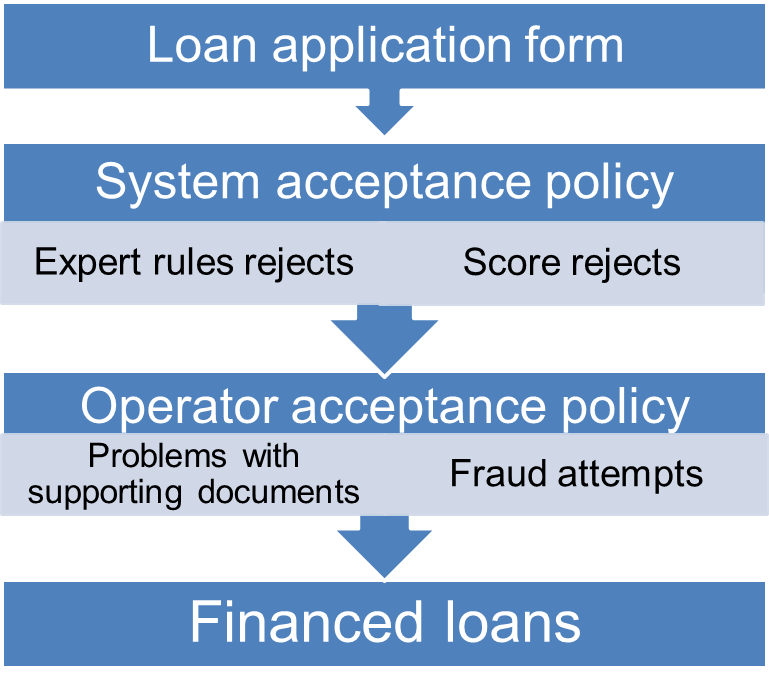
\includegraphics[width=5cm]{figures/schema.png}
\caption{Simplified Acceptance mechanism in~Crédit Agricole Consumer Finance}
\label{fig:figure1}

\end{minipage}%
\hfil \begin{minipage}[b]{0.5\linewidth}

\center 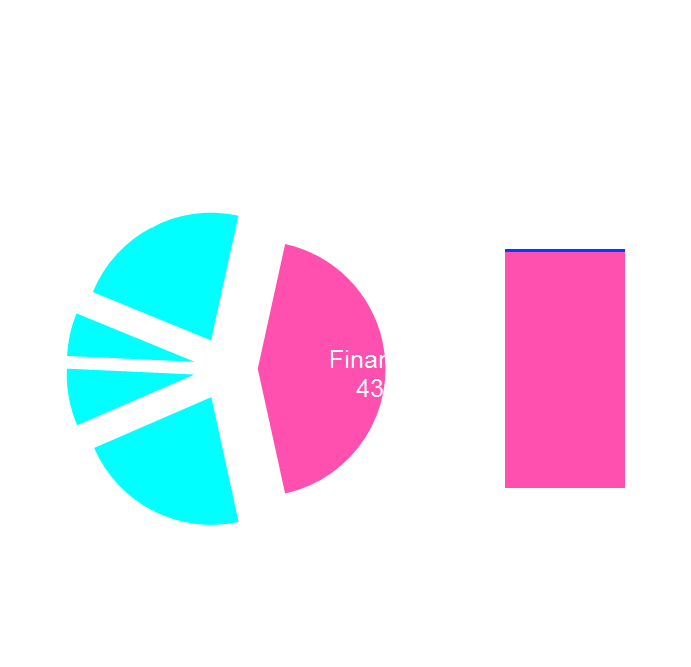
\includegraphics[width=5cm]{figures/camembert_invert.png}
\caption{Proportion of ``final'' lending decisions for CACF France}

\end{minipage}
\end{figure}

\end{frame}


\begin{frame}
\frametitle{\secname: \subsecname}

The observed data are the following:

\setbeamercolor{normal text}{fg=black}
\usebeamercolor[fg]{normal text}


\[ \hspace{-0.8cm} \textcolor{white}{\mathcal{T} =} \begin{array}{c}
\textcolor{white}{\mathcal{T}_{\f} = \bigg(} \; \tikzmarkin[hor=style green]{el02} \mathbf{x}_{\f} \tikzmarkend{el02} \\
%\\
\textcolor{white}{\cup} \\
%\\
\textcolor{white}{\mathcal{T}_{\nf} = \bigg(} \; \tikzmarkin[hor=style orange]{el-12} \mathbf{x}_{\nf} \tikzmarkend{el-12} \end{array}
%{\color{white} \bigg(} 
\begin{array}{ccc}
\tikzmarkin[hor=style green]{e1} \; \; x_{1,1} & \cdots & x_{1,d} \\
 \vdots & \vdots & \vdots  \\
 x_{n,1} & \cdots & x_{n,d} \tikzmarkend{e1} \\
\tikzmarkin[hor=style orange]{e2} \; \; x_{n+1,1} & \cdots & x_{n+1,d}  \\
 \vdots & \vdots & \vdots \\
 x_{n+n',1} & \cdots & x_{n+n',d} \tikzmarkend{e2} \end{array} %{\color{white} \bigg),}
 \hspace{0.5cm}
 \begin{array}{c}
\tikzmarkin[hor=style green]{el11} \mathbf{y}_{\f} \tikzmarkend{el11} \\
\\
\\
\\
\tikzmarkin[hor=style orange]{el12} \mathbf{y}_{\nf} \tikzmarkend{el12}\end{array}
%\left( 
\begin{array}{c}
\tikzmarkin[hor=style green]{e4} y_1 \\
\vdots \\
y_n \tikzmarkend{e4} \\ 
\tikzmarkin[hor=style orange]{e3} \text{NA} \\
\vdots \\
\text{NA} \tikzmarkend{e3} \end{array} %\textcolor{white}{\right),}
 \hspace{0.5cm}
 \begin{array}{c}
\tikzmarkin[hor=style green]{el5} \mathbf{z}_{\f} \tikzmarkend{el5} \\
\\
\\
\\
\tikzmarkin[hor=style orange]{el6} \mathbf{z}_{\nf} \tikzmarkend{el6} \end{array}
%\left( 
\begin{array}{c}
\tikzmarkin[hor=style green]{e8} \text{f} \\
\vdots \\
\text{f} \tikzmarkend{e8} \\ 
\tikzmarkin[hor=style orange]{e9} \text{nf} \\
\vdots \\
\text{nf} \tikzmarkend{e9} \end{array} % \right)
 \hspace{0.2cm}
 \begin{array}{c}
\textcolor{white}{\bigg).} \\
\\
%\\
\\
\textcolor{white}{\bigg).} \end{array}
\]
 
  
\setbeamercolor{normal text}{fg=white}
\usebeamercolor[fg]{normal text}



We traditionally build a logistic regression using only financed clients ({\bf fixed parameter space $\Theta$}):
\[ \hat{\bm{\theta}}_{\f} = \argmax_{\bm{\theta}} \ell(\bm{\theta} ; \mathcal{T}_\f), \]
which asymptotically approximates:
\[ \bm{\theta}_{\f}^\star = \argmin_{\bm{\theta}} \mathbb{E}_{\bm{X}} [\text{KL}(p || p_{\bm{\theta}}) | Z = \f]. \]

\end{frame}



\begin{frame}
\frametitle{\secname: \subsecname}

We wish we had:
\[ \hat{\bm{\theta}} = \argmax_{\bm{\theta}} \ell(\bm{\theta} ; \mathbf{x}, \mathbf{y}), \]
which asymptotically approximates:
\[ \bm{\theta}^\star = \argmin_{\bm{\theta}} \mathbb{E}_{\bm{X}} [\text{KL}(p || p_{\bm{\theta}})]. \]
But we lack $\mathbf{y}_{\nf}$.

\begin{center}
\resizebox{0.8\textwidth}{4.7cm}{
\begin{tikzpicture}[scale=1.1,every node/.style={minimum size=1cm},on grid]

	% Real level
	\begin{scope}[
		yshift=-120,
		every node/.append style={yslant=\yslant,xslant=\xslant},
		yslant=\yslant,xslant=\xslant
	] 
		% The frame:
		\draw[white, dashed, thin] (0,0) rectangle (7,7); 
		% Agents:
		\draw[fill=red]  
			(5,2) circle (.1) % Firms
			(2,2) circle (.1); % Households
		% Flows:
		\draw[-latex,thin, blue] 
			(2,2.2) to (2,4); % Labour Powers
		\draw[-latex,thin, blue]
			(4.85,1.85) to (4,1); % Wages
		 % Labels:
		\fill[white]
			(0.5,6.5) node[right, scale=2.5] {Model space $\Theta$}	
			(4.9,1.9) node[right,scale=2]{$\theta_{\f}^\star$}
			(2.1,1.9) node[below,scale=2]{$\theta^\star$}
			(2.2,4.3) node [scale=2] {$\hat{\theta}$} 
			(4.2,0.6) node [scale=2] {$\hat{\theta}_{\f}$};
		\fill[blue]
			(1,3) node [scale=1] {Estimation}
            (1,2.7) node [scale=1] {bias+variance};
		\fill[blue]
			(5.7,1.1) node [scale=1] {Estimation}
            (5.7,0.8) node [scale=1] {bias+variance};

	\end{scope}
	
	% 2 vertical lines for linking agents on the 2 levels
	\draw[thin, dashed, red](.8,1.75) to (3.8,-0.32);
	\draw[thin, dashed, red](.8,1.75) to (.8,-1.8);
	
    % Draw right angle scheme
    \draw(.8,-1.6) to (1,-1.6);
    \draw(1,-1.6) to (1,-1.8);


	% Monetary level
	\begin{scope}[
		yshift=-20,
		every node/.append style={yslant=0,xslant=0},
		yslant=\yslant,xslant=\xslant
	]
		 % Agents:
		\draw [fill=olive]
			(2,2) circle (.1); % Households
		 % Labels:
		\fill[black]
			(2.2,2.4) node[right,scale=2]{\textcolor{olive}{$p(y|\bm{x})$}};
%			(4,2) node[right,scale=2]{\textcolor{olive}{$p(y|\bm{x}, z = \f)$}};
        \fill[red]
			(0.85,0.35) node [right, scale=1.5] {Model bias};	

	\end{scope} 
\end{tikzpicture}
}
\end{center}


\end{frame}



\subsection{What is at stake?}

\begin{frame}
\frametitle{\secname : \subsecname}
\uncover<1->{
\textbf{Estimators :}

\begin{enumerate}
\only<1>{\item ‘‘Oracle'': $\sqrt[]{n+n'} ( \hat{\bm{\theta}} - \bm{\theta}^\star ) \xrightarrow[n,n' \to \infty]{\mathcal{L}} \mathcal{N}_{d+1} (0,{\Sigma}_{\bm{\theta}^\star})$}
\only<2>{\item ‘‘Oracle'': $\textcolor{red}{\sqrt[]{n+n'}} ( \hat{\bm{\theta}} - \bm{\theta}^\star ) \xrightarrow[n,n' \to \infty]{\mathcal{L}} \mathcal{N}_{d+1} (0,{\Sigma}_{\bm{\theta}^\star})$}
\only<3>{\item ‘‘Oracle'': $\sqrt[]{n+n'} ( \hat{\bm{\theta}} - \textcolor{red}{\bm{\theta}^\star} ) \xrightarrow[n,n' \to \infty]{\mathcal{L}} \mathcal{N}_{d+1} (0,{\Sigma}_{\bm{\theta}^\star})$}
\only<4>{\item ‘‘Oracle'': $\sqrt[]{n+n'} ( \hat{\bm{\theta}} - \bm{\theta}^\star ) \xrightarrow[n,n' \to \infty]{\mathcal{L}} \mathcal{N}_{d+1} (0,\textcolor{red}{{\Sigma}_{\bm{\theta}^\star}})$}
\only<5->{\item ‘‘Oracle'': $\textcolor{red}{\sqrt[]{n+n'}} ( \hat{\bm{\theta}} - \textcolor{red}{\bm{\theta}^\star} ) \xrightarrow[n,n' \to \infty]{\mathcal{L}} \mathcal{N}_{d+1} (0,\textcolor{red}{{\Sigma}_{\bm{\theta}^\star}})$}

\only<1>{\item Current methodology: $ \sqrt[]{n} ( \hat{\bm{\theta}}_{\f} - \bm{\theta}^\star_{\f} ) \xrightarrow[n \to \infty]{\mathcal{L}} \mathcal{N}_{d+1} (0,{\Sigma}_{\f,\bm{\theta}^\star_{\f}})$}
\only<2>{\item Current methodology: $ \textcolor{red}{\sqrt[]{n}} ( \hat{\bm{\theta}}_{\f} - \bm{\theta}^\star_{\f} ) \xrightarrow[n \to \infty]{\mathcal{L}} \mathcal{N}_{d+1} (0,{\Sigma}_{\f,\bm{\theta}^\star_{\f}})$}
\only<3>{\item Current methodology: $ \sqrt[]{n} ( \hat{\bm{\theta}}_{\f} - \textcolor{red}{\bm{\theta}^\star_{\f}} ) \xrightarrow[n \to \infty]{\mathcal{L}} \mathcal{N}_{d+1} (0,{\Sigma}_{\f,\bm{\theta}^\star_{\f}})$}
\only<4>{\item Current methodology: $ \sqrt[]{n} ( \hat{\bm{\theta}}_{\f} - \bm{\theta}^\star_{\f} ) \xrightarrow[n \to \infty]{\mathcal{L}} \mathcal{N}_{d+1} (0,\textcolor{red}{{\Sigma}_{\f,\bm{\theta}^\star_{\f}}})$}
\only<5->{\item Current methodology: $ \textcolor{red}{\sqrt[]{n}} ( \hat{\bm{\theta}}_{\f} - \textcolor{red}{\bm{\theta}^\star_{\f}} ) \xrightarrow[n \to \infty]{\mathcal{L}} \mathcal{N}_{d+1} (0,\textcolor{red}{{\Sigma}_{\f,\bm{\theta}^\star_{\f}}})$}

\end{enumerate}
}

\bigskip

\bigskip

\uncover<5->{
\textbf{\textcolor{red}{Question 1} :} asymptotics of the estimators

\centering{\fbox{(Q1) $ {\bm{\theta}}^\star \stackrel{?}{=} {{\bm{\theta}}}^\star_{\f} $}}

\fbox{(Q2) \centering{${\Sigma}_{\bm{\theta}^\star} \stackrel{?}{=} {\Sigma}_{\f,\bm{\theta}^\star_{\f}} $}}

}

\end{frame}

%----------------------------------------------------------------------------------------

\subsection*{Missingness mechanism}

\begin{frame}
\frametitle{\secname : \subsecname}

\begin{itemize}
\item \textbf{MAR} : $\forall \: x,y,z, \; p(z| \bm{x},y) = p(z| \bm{x})$

$\rightarrow$ Acceptance is determined by an old score: $Z = \mathds{1}_{\{\bm{\theta}'X > \text{cut}\}}$.

\item \textbf{MNAR} : $\exists \: x,y,z, \; p(z| \bm{x},y) \neq p(z| \bm{x})$

$\rightarrow$ Operators' ‘‘feeling'' $\tilde{\bm{X}}$ influence the acceptance.

$\rightarrow$ Expert rules based on features $\tilde{\bm{X}}$ not in $\bm{X}$.
\end{itemize}

\begin{figure}
\begin{tikzpicture}

\tikzset{vertex/.style = {shape=circle,draw,minimum size=1.5em}}
\tikzset{edge/.style = {->,> = latex'}}
% vertices
\node[vertex] (y) at  (0,0) {$Y$};
\node[vertex] (x) at  (2,0) {$\bm{X}$};
\node[vertex] (xc) at  (2,1) {$\tilde{\bm{X}}$};
\node[vertex] (z) at (4,0) {$Z$};

edges
\draw[edge] (y) to (x);
\draw[edge] (xc) to (x);
\draw[edge] (xc) to (z);
\draw[edge] (x) to (z);
\draw[dashed] (y) to (xc);

\end{tikzpicture}
\label{fig:mar}
\caption{Dependencies between random variables $Y$, $\bm{\tilde{X}}$, $\bm{X}$ and $Z$}
\end{figure}

\end{frame}

%----------------------------------------------------------------------------------------

\subsection*{Model specification}

\begin{frame}
\frametitle{\secname : \subsecname}

\begin{itemize}
\item \textbf{Well-specified model} : $p(y|\bm{x}) = p_{\bm{\theta}^\star}(y|\bm{x})$.

$\rightarrow$ With real data $\Rightarrow$ hypothesis unlikely to be true.
\item \textbf{Misspecified model} : $\bm{\theta}^\star$ is the ``best'' in the $\Theta$ family.

$\rightarrow$ Logistic regression commonly used for its robustness to misspecification (no assumption about $p(\bm{x})$).
\end{itemize}

\footnotesize{
\begin{table}[ht]
\begin{tabular}{|R{3.4cm}||C{2cm}|C{2cm}|}
\hline \backslashbox{$p_{\bm{\theta}}(y|\bm{x})$}{$p(z|\bm{x},y)$} & MAR & MNAR \\
\hline
\hline \multirow{2}{*}{Well specified} & $\textcolor{olive}{\bm{\theta}^\star_{\f} = \bm{\theta}^\star}$ &  \\ 
  & ${\Sigma}_{\f,\bm{\theta}^\star_{\f}} \neq {\Sigma}_{\theta^\star}$ & \textcolor{red}{$\bm{\theta}^\star_{\f} \neq \bm{\theta}^\star$} \\ \cline{1-2}
 \multirow{2}{*}{Misspecified} & \textcolor{red}{$\bm{\theta}^\star_{\f} \neq \bm{\theta}^\star$} & \textcolor{red}{${\Sigma}_{\f,\bm{\theta}^\star_{\f}} \neq {\Sigma}_{\theta^\star}$} \\
 & \textcolor{red}{${\Sigma}_{\f,\bm{\theta}^\star_{\f}} \neq {\Sigma}_{\theta^\star}$} &  \\
\hline 
\end{tabular}
\label{tableasymptotic}
\caption{(Q1) and (Q2) w.r.t. model specification and missingness mechanism}
\end{table}
}

\end{frame}

%----------------------------------------------------------------------------------------

\subsection{How to use $\mathbf{x}_{\nf}$?}

\begin{frame}
\frametitle{\secname : \subsecname}

\uncover<1->{
\textbf{\textcolor{red}{Question 2}:} How to construct a better estimator than $\hat{\bm{\theta}}_{\f}$?
}

\bigskip

\bigskip

\uncover<2->{
\textbf{\textcolor{red}{Scope for action}:}
}
\begin{itemize}
\only<2-5>{\item Change model space $\Theta$,}
\only<6->{\item \sout{Change model space $\Theta$} logistic regression,}
\only<3-6>{\item Model acceptance/rejection process (i.e. $p_{\gamma}(z|\bm{x},y)$),}
\only<7->{\item \sout{Model acceptance/rejection process (i.e. $p_{\gamma}(z|\bm{x},y)$)}

$\gamma$ cannot be estimated,}
\item<4-> Use $\mathbf{x}_{\nf}$.
\end{itemize}

\only<5>{
\begin{block}{Natural way to achieve all three: generative approach}
\setlength\abovedisplayskip{-5pt}
\begin{flalign*}
& \hspace{0.4cm} {p_{\textcolor{red}{\alpha}}(\bm{x},y,z) = p_{\beta_{\textcolor{red}{\alpha}}}(\bm{x}) p_{\theta_{\textcolor{red}{\alpha}}}(y|x) p_{\gamma_{\textcolor{red}{\alpha}}}(z|\bm{x},y).} &
\end{flalign*}
\begin{alignat*}{2}
& (\fbox{$\hat{\theta}_{\textcolor{red}{\alpha}}$},\hat{\beta}_{\textcolor{red}{\alpha}},\hat{\gamma}_{\textcolor{red}{\alpha}}) && = \argmax_{{{\theta}_{\textcolor{red}{\alpha}}},\beta_{\textcolor{red}{\alpha}},\gamma_{\textcolor{red}{\alpha}}} \ell({\textcolor{red}{\alpha}};\bm{x},\bm{y}_{\f}) = \argmax_{{{\theta}_{\textcolor{red}{\alpha}}},\beta_{\textcolor{red}{\alpha}},\gamma_{\textcolor{red}{\alpha}}} \sum_{i=1}^{n }\ln(p_{\theta_{\textcolor{red}{\alpha}}}(y_i|x_i)) \\
& && + \sum_{i=1}^{n+n'} \ln(p_{\beta_{\textcolor{red}{\alpha}}}(\bm{x}_i)) \left( + \sum_{i=1}^{n} \ln(p_{\gamma_{\textcolor{red}{\alpha}}}(z_i|x_i,y_i)) \right).
\end{alignat*}
\end{block}
}
\only<6>{
\begin{block}{\sout{Natural way to achieve all three: generative approach}}
\setlength\abovedisplayskip{-5pt}
\begin{flalign*}
& \hspace{0.4cm} {p_{\textcolor{red}{\alpha}}(\bm{x},y,z) = p_{\beta_{\textcolor{red}{\alpha}}}(\bm{x}) p_{\theta_{\textcolor{red}{\alpha}}}(y|\bm{x}) p_{\gamma_{\textcolor{red}{\alpha}}}(z|\bm{x},y).} &
\end{flalign*}
\begin{alignat*}{2}
& (\fbox{$\hat{\theta}_{\textcolor{red}{\alpha}}$},\hat{\beta}_{\textcolor{red}{\alpha}},\hat{\gamma}_{\textcolor{red}{\alpha}}) && = \argmax_{\textcolor{red}{\alpha}} \ell({\textcolor{red}{\alpha}};\bm{x},\bm{y}_{\f}) = \argmax_{{{\theta}_{\textcolor{red}{\alpha}}},\beta_{\textcolor{red}{\alpha}},\gamma_{\textcolor{red}{\alpha}}} \sum_{i=1}^{n}\ln(p_{\theta_{\textcolor{red}{\alpha}}}(y_i|x_i)) \\
& && + \sum_{i=1}^{n+n'} \ln(p_{\beta_{\textcolor{red}{\alpha}}}(\bm{x}_i)) \left( + \sum_{i=1}^{n} \ln(p_{\gamma_{\textcolor{red}{\alpha}}}(z_i|x_i,y_i)) \right).
\end{alignat*}
\end{block}
}

\uncover<8->{
%\begin{tikzpicture}
%\coordinate (A) at (-1,1);
%\coordinate (B) at (3,0.5);
%\coordinate (C) at (4,-1);
%\coordinate (D) at (1,-1);
%\foreach \p in {A,B,C,D}
%{\draw[fill=white] (\p) circle (1pt);}
%\DrawPotato[blue,fill=red]{A}{B}{C}{D}
%\end{tikzpicture}

{\bf Remember} that $\mathcal{T}^{\text{OOT}}$ also comes from $p(y | \bm{x}, \f)$ such that applying a \textit{Reject Inference} method and getting a higher Gini is no guarantee that it would on the Through-the-Door population (on the contrary!).
}

\end{frame}





\begin{frame}
\frametitle{\secname: \subsecname}

For logistic regression, \textit{Reject Inference} methods amount to:
\setbeamercolor{normal text}{fg=black}
\usebeamercolor[fg]{normal text}
\hspace*{-0.7cm} \[ \textcolor{white}{\mathcal{T}_{\text{c}}^{(1)} = } %\left(
\begin{array}{c}
\tikzmarkin[hor=style green]{el0} \mathbf{x}_{\f} \tikzmarkend{el0} \\
\\
\\
\tikzmarkin[hor=style green]{el-1} \mathbf{x}_{\nf} \tikzmarkend{el-1} \end{array}
%\left( 
\begin{array}{ccc}
\tikzmarkin[hor=style green]{el1} \; \; x_{1,1} & \cdots & x_{1,d}  \\
 \vdots & \vdots & \vdots \\
 x_{n,1} & \cdots & x_{n,d} \\
 x_{n+1,1} & \cdots & x_{n+1,d}  \\
 \vdots & \vdots & \vdots \\
 x_{n+n',1} & \cdots & x_{n+n',d} \tikzmarkend{el1} \end{array},
 \hspace{0.2cm}
 \begin{array}{c}
\tikzmarkin[hor=style green]{l1} \mathbf{y}_{\f} \tikzmarkend{l1}\\
\\
\\
\tikzmarkin[hor=style green]{l2} \mathbf{y}_{\nf} \tikzmarkend{l2} \end{array}
%\left( 
\begin{array}{c}
\tikzmarkin[hor=style green]{l3} \; \; y_1 \; \; \; \\
\vdots \\
 y_n \\ 
 \hat{y}_{n+1}^{(1)} \\
\vdots \\
\hat{y}_{n+n'}^{(1)} \tikzmarkend{l3}\end{array},
\hspace{0.2cm} 
 \begin{array}{c}
\tikzmarkin[hor=style green]{el111} \mathbf{z}_{\f} \tikzmarkend{el111}\\
\\
\\
\tikzmarkin[hor=style green]{el121} \mathbf{z}_{\nf} \tikzmarkend{el121}\end{array}
%\left( 
\begin{array}{c}
\tikzmarkin[hor=style green]{e41} \text{f} \\
\vdots \\
\text{f} \\ 
\text{nf} \\
\vdots \\
\text{nf} \tikzmarkend{e41} \end{array}.\]
 
\setbeamercolor{normal text}{fg=white}
\usebeamercolor[fg]{normal text}

\end{frame}

 
 
 
 
 
 \begin{frame}
\frametitle{\secname : \subsecname}

\textbf{Reclassification}\footnote{\cite{RI6,banasik,saporta}} :
\[(\hat{\bm{\theta}}^{\text{CEM}}, \textcolor{red}{\hat{\mathbf{y}}^{\nf}}) = \argmax_{\bm{\theta},\textcolor{red}{\mathbf{{y}}^{\nf}}} \ell(\bm{\theta}; \mathcal{T}_c^{(1)}) \text{ where } \textcolor{red}{\hat{y_i}} = \argmax_{y_i} p_{\hat{\bm{\theta}}_{\f}}(y_i|\bm{x}_i).\]
\textbf{Problem:} inconsistent estimator.

\vspace*{0.2cm}
\hspace*{-0.8cm} \centering 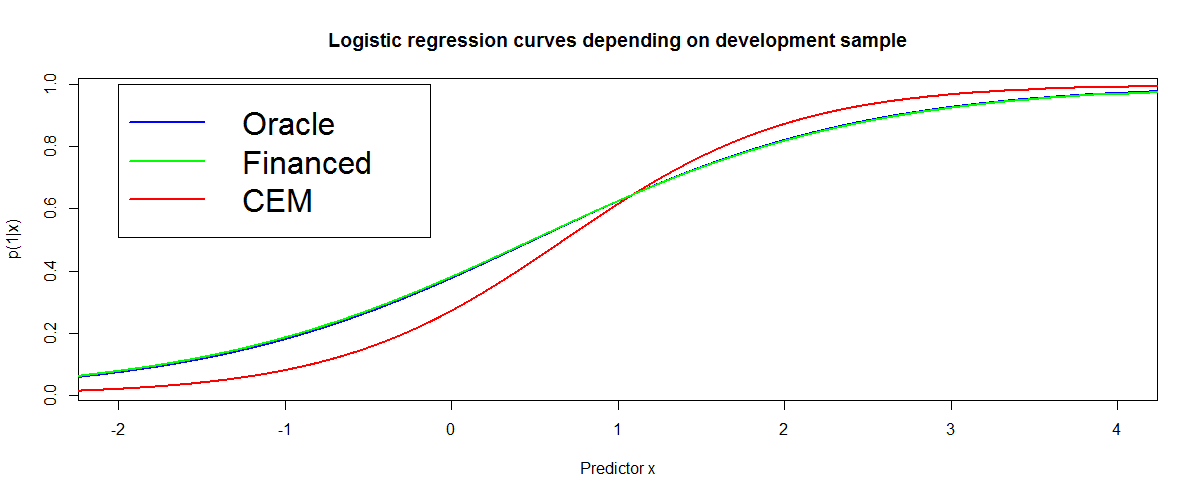
\includegraphics[width=12cm]{figures/CEM_bias.png}

\end{frame}

%----------------------------------------------------------------------------------------

\begin{frame}
\frametitle{\secname : \subsecname}

\textbf{Augmentation}\footnote{\cite{RI6,banasik,saporta,economix}}: MAR / misspecified model.
\[ \ell_{\text{Aug}}(\bm{\theta}; \mathcal{T}_\f) = \sum_{i=1}^n \textcolor{red}{\frac{1}{p(\text{f}|\bm{x}_i)}} \ln(p_{\bm{\theta}}(y_i|\bm{x}_i)).\]
\textbf{Problem:} estimation of $p(\text{f}|x_i)$ + assumes $p(\text{f}|x_i) > 0$ (clearly not true).

\medskip

\noindent\makebox[\linewidth]{\rule{\paperwidth}{1pt}}

\medskip

\textbf{Parcelling} \footnote{\cite{RI6,banasik,saporta}}:
\[ \ell(\theta; \bm{x},\mathbf{y}_{\f},\textcolor{red}{\mathbf{\hat{y}}_{\nf}}) \text{ where } \textcolor{red}{\hat{y_i}} = \begin{cases} 1 \text{ w.p. } \textcolor{red}{\alpha_i} p_{\hat{\bm{\theta}}_{\f}}(1|\bm{x}_i,\text{f}) \\ 0 \text{ w.p. } 1-\textcolor{red}{\alpha_i} p_{\hat{\bm{\theta}}_{\f}}(1|\bm{x}_i,\text{f}) \end{cases}. \]

\textbf{Problem:} MNAR assumptions hidden in $\textcolor{red}{\mathbf{\hat{y}}_{\nf}}$ ($\textcolor{red}{\alpha_i}$) impossible to test.

\end{frame}



 
\subsection{Additional remarks} 
 
\begin{frame}
\frametitle{\secname: \subsecname}

\begin{animateinline}[autoplay,loop]{2}%
{\color{red}{\bf WARNING}}%
\newframe \end{animateinline}

\medskip

All this stands for logistic regression and all ``local'' methods~\cite{zadrozny2004learning}.

\medskip

All ``global'' methods (explicit or implicit modelling of $p(\bm{x})$) will produce biased estimates under MAR.

\medskip

We might have:

\begin{table}[t]
\centering
\begin{tabular}{l || l | l}
Gini & Logistic regression & Decision trees \\
\hline
Financed & 40 & 45 \\
\textcolor{red}{Through-the-door} & 40 & 35 \\
\end{tabular}
\end{table}

\end{frame}






\section{Feature quantization}


\subsection{By an example}

{
\setbeamercolor{background canvas}{bg=white}
\begin{frame}
\frametitle{\secname: \subsecname}

\begin{figure}[!ht]
\begin{animateinline}[poster=first, controls=all, palindrome, autopause, autoresume, width=\textwidth, height=6cm]{3}
\multiframe{99}{i=2+1}{\input{CODE_FIGURES/EXAMPLE_DISC/disc_plot\i.tex}}%
\end{animateinline}
\end{figure}

\end{frame}
}


\subsection{Some more notations}

\begin{frame}[allowframebreaks]
\frametitle{\subsecname}

\begin{block}{Raw data}
\vspace*{-0.9cm}
\begin{align*}
\bx & =(x_1,\dots,x_d) \\
x_j & \in \mathbb{R} \text{ (continuous case)} \\
x_j & \in \{1,\dots,l_j\} \text{ (categorical case)} \\
y & \in \{0,1\} \text{ (target)}
\end{align*}
\vspace*{-0.7cm}
\end{block}

\bigskip

\begin{block}{Quantized data}
\vspace*{-0.9cm}
\begin{align*}
\q(\bx) & = (\q_1(x_1),\dots,\q_d(x_d)) \\
\q_j(x_j) & = (\s_{j,h}(x_j))_1^{m_j} \text{ (one-hot encoding)} \\
\s_{j,h}(\cdot) & =  1 \text{ if } x_j \in C_{j,h}, 0 \text{ otherwise, } 1 \leq h \leq m_j
\end{align*}
\vspace*{-0.7cm}
\end{block}

\pagebreak

\begin{block}{Discretization}
\vspace*{-0.4cm}
\[C_{j,h}=(c_{j,h-1},c_{j,h}]\]

where $c_{j,1},\ldots,c_{j,m_j-1}$ are increasing numbers called cutpoints, $c_{j,0}=-\infty$ and $c_{j,m_j}=+\infty$.
\end{block}

\bigskip

\begin{center}
\begin{tikzpicture}[scale=0.3]
\draw[->,line width=0.1cm] (-5,0)--(24,0) node[right]{$x_j$};

\node [red,circle, fill] at (4,0) {};
\node [red,circle, fill] at (12,0) {};

\node at (4,-1.5) {$c_{j,1}$};
\node at (12,-1.5) {$c_{j,2}$};

\node at (-1,1) {$(1,0,0)$};
\node at (8,1) {$(0,1,0)$};
\node at (19,1) {$(0,0,1)$};

\end{tikzpicture}
\end{center}

\pagebreak

\begin{block}{Grouping}
\vspace*{-0.4cm}
\[\bigsqcup_{h=1}^{m_j}C_{j,h}=\{1,\ldots,l_j\}.\]
\vspace*{-0.2cm}
\end{block}

\bigskip

\begin{center}
\begin{tikzpicture}[scale=0.25,every node/.style={scale=0.9}]
\tikzset{vertex/.style = {shape=circle,draw,scale=0.7,minimum size=1cm}}
\tikzset{edge/.style = {->,> = latex'}}

% Boules E^j
\node [vertex] (e1) at (3,4) {$(1,0)$};
\node [vertex] (e2) at (15,4) {$(0,1)$};

% Boules X^J
\node [vertex] (x1) at (-4,0) {1};
\node [vertex] (x2) at (1.8,0) {2};
\node [vertex] (x3) at (9.5,0) {3};
\node [vertex] (x4) at (17,0) {4};
\node [vertex] (x5) at (24,0) {5};

% Labels
\node at (-7,4) {$\q_j(x_j)=$};
\node at (-7,0) {$x_j=$};

% Flèches
\draw[edge,line width=0.03cm] (x1) to (e1);
\draw[edge,line width=0.03cm] (x3) to (e1);
\draw[edge,line width=0.03cm] (x4) to (e1);
\draw[edge,line width=0.03cm] (x2) to (e2);
\draw[edge,line width=0.03cm] (x5) to (e2);

\end{tikzpicture}
\end{center}

\end{frame}






\subsection{Existing approaches}
\begin{frame}
\frametitle{\secname: \subsecname}

\vspace*{-0.1cm}
\centering 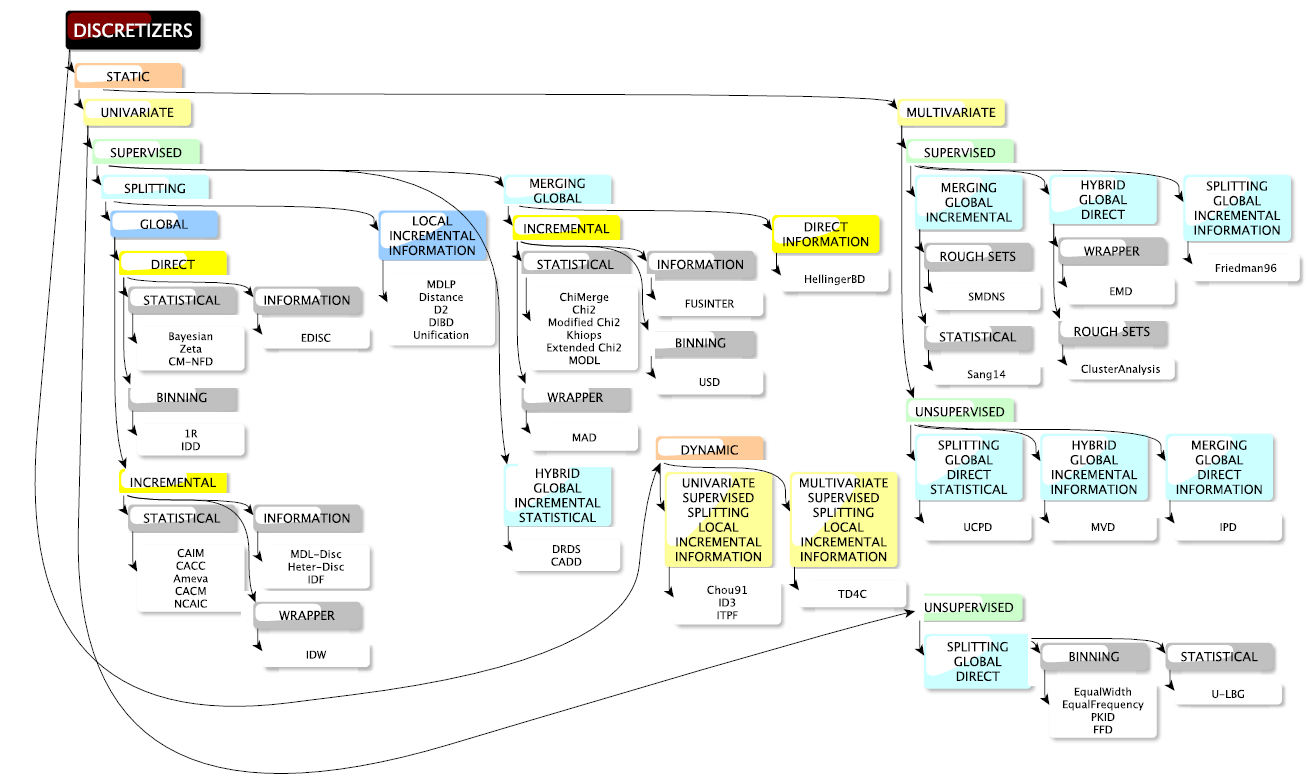
\includegraphics[scale=0.25]{figures/taxonomy.PNG}

You maximize an \textit{ad hoc} criterion:
\vspace*{-0.1cm}
\[ \hat{\q} = \argmax_{\q} \text{CRIT}(\mathcal{T}_\f), \]
\vspace*{-0.1cm}
and {\bf hope} that it's aligned with your original goal:
\vspace*{-0.1cm}
\[ \hat{\bm{\theta}}_{\hat{\q}} = \argmax_{\bm{\theta}_{\hat{\q}}} \ell(\bm{\theta}_{\hat{\q}} ; \mathcal{T}_\f). \]

\end{frame}





\subsection{Approximation}
\begin{frame}
\frametitle{\secname: \subsecname}

\begin{equation*}
    \q_{\ag_j}(\cdot)=\left(q_{\ag_{j,h}}(\cdot)\right)_{h=1}^{m_j} \text{ with } \begin{cases} \sum_{h=1}^{m_j}q_{\ag_{j,h}}(\cdot)=1, \\ 0 \leq q_{\ag_{j,h}}(\cdot) \leq 1, \end{cases}
\end{equation*}

\uncover<2->{

\textbf{For continuous features}, we set for $\bm{\alpha}_{j,h} = (\alpha^0_{j,h},\alpha^1_{j,h}) \in \mathbb{R}^2$
\[\s_{\ag_{j,h}}(\cdot) = \frac{\exp(\alpha^0_{j,h} + \alpha^1_{j,h}  \cdot)}{\sum_{g=1}^{m_j} \exp(\alpha^0_{j,g} + \alpha^1_{j,g}  \cdot)}.\]
\textbf{For categorical features}, we set for $\bm{\alpha}_{j,h}=\left(\alpha_{j,h}(1),\ldots, \alpha_{j,h}(l_j)\right) \in \mathbb{R}^{l_j}$
\[\s_{\ag_{j,h}}(\cdot) = \frac{\exp\left(\alpha_{j,h}(\cdot)\right)}{\sum_{g=1}^{m_j} \exp\left(\alpha_{j,g}(\cdot)\right)}.\]

}

\end{frame}





\subsection{Estimation MAP}
\begin{frame}
\frametitle{\secname : \subsecname}

\[ {\s}^{\text{MAP}}_{j,h}(x_j) = 1 \text{ if } h = \argmax_{1 \leq h' \leq m_j} \s_{\hat{\ag}_{j,h'}}, 0 \text{ otherwise.} \]

\begin{tikzpicture}[scale=0.9]
\begin{axis}[
  no markers, domain=-1.5:2, samples=100,
  axis lines*=left,
  every axis y label/.style={at=(current axis.left of origin), anchor=north west},
  height=3cm, width=11cm,
  xtick=\empty, ytick=\empty,
  enlargelimits=false, clip=false,
  x label style={at={(axis description cs:0.5,-0.1)},anchor=north},
  y label style={at={(axis description cs:-0.1,.5)},rotate=90,anchor=south},
  xlabel={$x_j$},
  ylabel={$\s_{\hat{\ag}_{j,1}}(x_j)$}
  ]
    
  \addplot [very thick,white] {gauss(-1.8,0.6)};
\addplot+[mark=none,thick,red] coordinates {(-0.7,0) (-0.7,0.6)};
\addplot+[mark=none,thick,red] coordinates {(1,0) (1,0.6)};
\node at (axis cs:-1.1,0.4) {$\hat{\s}_{j,1}(x_j)=1$};
\node at (axis cs:0,0.4) {$\hat{\s}_{j,1}(x_j)=0$};
\node at (axis cs:1.5,0.4) {$\hat{\s}_{j,1}(x_j)=0$};
\node at (axis cs:-0.7,-0.15) {$\hat{c}_{j,1}$};
\node at (axis cs:1,-0.15) {$\hat{c}_{j,2}$};

\end{axis}
\end{tikzpicture}

\begin{tikzpicture}[scale=0.9]
\begin{axis}[
  no markers, domain=-1.5:2, samples=100,
  axis lines*=left,
  every axis y label/.style={at=(current axis.left of origin), anchor=north west},
  height=3cm, width=11cm,
  xtick=\empty, ytick=\empty,
  enlargelimits=false, clip=false,
  x label style={at={(axis description cs:0.5,-0.1)},anchor=north},
  y label style={at={(axis description cs:-0.1,.5)},rotate=90,anchor=south},
  xlabel={$x_j$},
  ylabel={$\s_{\hat{\ag}_{j,2}}(x_j)$}
  ]
    
  \addplot [very thick,white] {gauss(0,0.6)};
\addplot+[mark=none, thick,red] coordinates {(-0.7,0) (-0.7,0.6)};
\addplot+[mark=none, thick,red] coordinates {(1,0) (1,0.6)};
\node at (axis cs:-1.1,0.4) {$\hat{\s}_{j,2}(x_j)=0$};
\node at (axis cs:0,0.4) {$\hat{\s}_{j,2}(x_j)=1$};
\node at (axis cs:1.5,0.4) {$\hat{\s}_{j,2}(x_j)=0$};
\node at (axis cs:-0.7,-0.15) {$\hat{c}_{j,1}$};
\node at (axis cs:1,-0.15) {$\hat{c}_{j,2}$};

\end{axis}

\end{tikzpicture}

\begin{tikzpicture}[scale=0.9]
\begin{axis}[
  no markers, domain=-1.5:2, samples=100,
  axis lines*=left,
  every axis y label/.style={at=(current axis.left of origin), anchor=north west},
  height=3cm, width=11cm,
  xtick=\empty, ytick=\empty,
  enlargelimits=false, clip=false,
  x label style={at={(axis description cs:0.5,-0.1)},anchor=north},
  y label style={at={(axis description cs:-0.1,.5)},rotate=90,anchor=south},
  xlabel={$x_j$},
  ylabel={$\s_{\hat{\ag}_{j,3}}(x_j)$}
  ]
    
  \addplot [very thick,white] {gauss(2,0.6)};

\addplot+[mark=none, thick,red] coordinates {(-0.7,0) (-0.7,0.6)};
\addplot+[mark=none, thick,red] coordinates {(1,0) (1,0.6)};

\node at (axis cs:-1.1,0.4) {$\hat{\s}_{j,3}(x_j)=0$};
\node at (axis cs:0,0.4) {$\hat{\s}_{j,3}(x_j)=0$};
\node at (axis cs:1.5,0.4) {$\hat{\s}_{j,3}(x_j)=1$};
\node at (axis cs:-0.7,-0.15) {$\hat{c}_{j,1}$};
\node at (axis cs:1,-0.15) {$\hat{c}_{j,2}$};

\end{axis}
\end{tikzpicture}


\end{frame}





\subsection{Neural networks}

\begin{frame}
\frametitle{\secname: \subsecname}

We wish to maximize the following likelihood:
\[ (\hat{\bm{\theta}}, \hat{\bm{\alpha}}) = \argmax_{\bm{\theta}, \bm{\alpha}} \ell(\bm{\theta}, \bm{\alpha} ; \bm{x}, \bm{y}) = \sum_{i=1}^n p_{\bm{\theta}}(y_i | \q_{\alpha}(\bm{x}_i)). \]

\medskip

{\bf If there is a true quantization} $\q^\star$, then $\bm{\alpha}^\star = \lim_{n \to \infty} \hat{\bm{\alpha}}$ is such that $\q_{\bm{\alpha}^\star} = \q^\star$.

\medskip

\uncover<2->{
{\bf If not}, ${\q}^{\text{MAP}}$ is ``guaranteed'' to be a good candidate quantization.
}

\medskip

\uncover<3->{
{\bf Problem:} $\ell(\bm{\theta}, \bm{\alpha} ; \bm{x}, \bm{y})$ cannot be directly maximized (it's not even convex).
}

\medskip

\uncover<4->{
{\bf Solution:} Resort to gradient descent (not guaranteed to converge to a global maximum!).
}

\end{frame}






\begin{frame}
\frametitle{\secname: \subsecname}

\def\layersep{2.5cm}

\centering
\begin{tikzpicture}[shorten >=1pt,->,draw=black!50, node distance=\layersep]
    \tikzstyle{every pin edge}=[<-,shorten <=1pt]
    \tikzstyle{neuron}=[circle,fill=black!25,minimum size=17pt,inner sep=0pt]
    \tikzstyle{input neuron}=[neuron, fill=green!50];
    \tikzstyle{output neuron}=[neuron, fill=red!50];
    \tikzstyle{hidden neuron}=[neuron, fill=blue!50];
    \tikzstyle{annot} = [text width=4em, text centered]
    \tikzstyle{annotrectangle} = [text width=8em, text centered]


        \node[input neuron, pin=left:Continuous input \#1] (I-1) at (0,-1) {};
        
        \node[input neuron, pin=left:Level \#1] (I-2) at (0,-2) {};
        \node[input neuron, pin=left:Level \#2] (I-3) at (0,-3) {};
        \node[input neuron, pin=left:Level \#3] (I-4) at (0,-4) {};

    % Draw the hidden layer nodes
    \foreach \name / \y in {1,...,2}
        \path[yshift=0.5cm]
            node[hidden neuron] (H-\name) at (\layersep,-\y cm) {Soft};

    \foreach \name / \y in {3,...,4}
        \path[yshift=0.5cm]
            node[hidden neuron] (H-\name) at (\layersep,-\y cm) {Soft};

    % Draw the output layer node
    \node[output neuron,pin={[pin edge={->}]right:Output}, right of=H-2] (O) {$\sigma$};

    % Connect every node in the input layer with every node in the
    % hidden layer.
%    \foreach \source in {1,...,4}
        \foreach \dest in {1,2}
            \path (I-1) edge (H-\dest);

        \foreach \dest in {3,4}
            \path (I-2) edge (H-\dest);
        \foreach \dest in {3,4}
            \path (I-3) edge (H-\dest);
        \foreach \dest in {3,4}
            \path (I-4) edge (H-\dest);

        % \foreach \dest in {5,6}
        %     \path (I-3) edge (H-\dest);

    % Connect every node in the hidden layer with the output layer
    \foreach \source in {1,...,4}
        \path (H-\source) edge (O);

    % Annotate the layers
    \node[annot,above of=H-1, node distance=1cm] (hl) {Hidden layer};
    \node[annot,left of=hl] {Input layer};
    \node[annot,right of=hl] {Output layer};
    
    
    \draw [orange] (2,0) rectangle (3,-1.9);
    % \draw [red] (2,-2) rectangle (3,-4);
    
    \node[annotrectangle,right of=H-1, node distance=2.5cm] {Softmax outputs are $\q_{{\ag}_j}(x_j)$.}; 
    

\end{tikzpicture}

\end{frame}





\begin{frame}
\frametitle{Estimation \textit{via} neural networks}

% \newlength\figureheight
% \newlength\figurewidth
% \setlength\figureheight{3cm}
% \setlength\figurewidth{\textwidth}


%  \begin{figure}[!ht]
%    \centering
%    \begin{subfigure}[t]{\textwidth}
%        \centering
%        % This file was created by matplotlib2tikz v0.6.18.
\begin{tikzpicture}

\definecolor{color0}{rgb}{0,0.75,0.75}
\definecolor{color1}{rgb}{0.75,0,0.75}
\definecolor{color2}{rgb}{0.75,0.75,0}

\begin{axis}[
height=\figureheight,
legend cell align={left},
legend entries={{${q}_{\bm{\alpha}_{1,1}}$},{${q}_{\bm{\alpha}_{1,2}}$},{${q}_{\bm{\alpha}_{1,3}}$},{${q}_{\bm{\alpha}_{1,4}}$},{${q}_{\bm{\alpha}_{1,5}}$},{$c_{1,1}$},{$c_{1,2}$},{$\hat{c}_{0,2}$}},
legend style={at={(0.91,0.5)}, anchor=east, draw=white, fill=black},
tick align=outside,
tick pos=left,
title={Continuous feature 1 at iteration 5},
width=\figurewidth,
x grid style={white!69.01960784313725!black},
xlabel={$x_1$},
xmin=0, xmax=1,
y grid style={white!69.01960784313725!black},
ylabel={${q}_{\bm{\alpha}_{0,h}}$},
ymin=0, ymax=1
]
\addlegendimage{no markers, red}
\addlegendimage{no markers, color0}
\addlegendimage{no markers, color1}
\addlegendimage{no markers, color2}
\addlegendimage{no markers, white}
\addlegendimage{no markers, dashed, green!50.0!black}
\addlegendimage{no markers, dashed, blue}
\addlegendimage{no markers, blue}
\addplot [thick, red]
table [row sep=\\]{%
0.0011059794751318	0.990096211433411 \\
0.00144600828615515	0.990088164806366 \\
0.00151620394328711	0.990086495876312 \\
0.00161381928831428	0.990084171295166 \\
0.00193644961641948	0.99007648229599 \\
0.0024363370221504	0.990064680576324 \\
0.00384167794354173	0.990030884742737 \\
0.00421063900202368	0.990022242069244 \\
0.00632372037002726	0.989971518516541 \\
0.00947686783375368	0.989895045757294 \\
0.0099356428556221	0.989883720874786 \\
0.0101317191976503	0.989879012107849 \\
0.0102519961026396	0.989876091480255 \\
0.0116572936797861	0.989841759204865 \\
0.0122763055741271	0.989826560020447 \\
0.0128807282915644	0.989811718463898 \\
0.0131006826676461	0.989806354045868 \\
0.0132105085232722	0.989803791046143 \\
0.0150477352877949	0.989758253097534 \\
0.0151511241047927	0.989755690097809 \\
0.0168553495563415	0.989713549613953 \\
0.0191895991753259	0.989655137062073 \\
0.0192724193499449	0.989653170108795 \\
0.0202131188025382	0.989629566669464 \\
0.0251886934986562	0.989503502845764 \\
0.0255409812646521	0.989494621753693 \\
0.0256196546755231	0.989492535591125 \\
0.0263800727822662	0.989473164081573 \\
0.026825697968402	0.989461719989777 \\
0.0272388337061176	0.989451229572296 \\
0.0276781997826389	0.989439904689789 \\
0.0277969734855988	0.989436745643616 \\
0.027888291941232	0.98943430185318 \\
0.032801074197002	0.989307105541229 \\
0.0337126623182875	0.989283204078674 \\
0.0349109578825388	0.989251792430878 \\
0.0367757145561887	0.989202558994293 \\
0.0368887253476963	0.989199638366699 \\
0.0376301111814882	0.989180088043213 \\
0.0383020767002249	0.989162087440491 \\
0.0385765124363792	0.989154756069183 \\
0.0386281055032889	0.989153444766998 \\
0.0397134557815922	0.989124536514282 \\
0.0400530872540832	0.989115476608276 \\
0.0408224228009035	0.989094793796539 \\
0.042416614098386	0.989051878452301 \\
0.042542997860721	0.989048600196838 \\
0.0425634328976269	0.989048182964325 \\
0.0426938593122377	0.989044547080994 \\
0.0436353215690566	0.989019095897675 \\
0.0476491609572692	0.988909900188446 \\
0.0476764809468383	0.988909184932709 \\
0.0480632979275277	0.988898575305939 \\
0.0489335324060199	0.988874673843384 \\
0.0494953541501341	0.988859176635742 \\
0.0498656975684827	0.988848924636841 \\
0.0507299142819697	0.988825023174286 \\
0.0520149216066462	0.988789319992065 \\
0.053491737186121	0.98874819278717 \\
0.0545456118282759	0.988718867301941 \\
0.0549368100196436	0.988707900047302 \\
0.0549667939602374	0.988706946372986 \\
0.0555159955251522	0.988691568374634 \\
0.0574839546417889	0.988636016845703 \\
0.0576927502423773	0.988630056381226 \\
0.0580609228746025	0.988619565963745 \\
0.0610070220733733	0.988535583019257 \\
0.0613718310828713	0.988525211811066 \\
0.0624819644863142	0.988493263721466 \\
0.0632024977130776	0.988472521305084 \\
0.0641707318537266	0.988444447517395 \\
0.064803290117067	0.988426208496094 \\
0.0661546388560771	0.988386809825897 \\
0.0675945492445934	0.988344788551331 \\
0.0701208744758773	0.988270401954651 \\
0.0704495440664726	0.988260746002197 \\
0.0707913481046274	0.988250613212585 \\
0.0709503961374458	0.988245725631714 \\
0.0723079949898875	0.988205313682556 \\
0.0729582139062805	0.988186001777649 \\
0.0736427592129116	0.988165497779846 \\
0.0738431652021745	0.988159537315369 \\
0.074094042941424	0.988152086734772 \\
0.0741988699821797	0.988148748874664 \\
0.0745344402647278	0.988138735294342 \\
0.0761651718345726	0.988089501857758 \\
0.0762565104011357	0.988086819648743 \\
0.0764247618188199	0.988081812858582 \\
0.0780473992355428	0.988032579421997 \\
0.0784939963588281	0.988018870353699 \\
0.0787288834363844	0.988011837005615 \\
0.0796528614743472	0.987983345985413 \\
0.0821291956626848	0.987907350063324 \\
0.0836539892117674	0.987860023975372 \\
0.0837976822096664	0.987855732440948 \\
0.0840863722935196	0.987846791744232 \\
0.0847664004367794	0.987825334072113 \\
0.0848642352310873	0.987822473049164 \\
0.0852150851090396	0.987811505794525 \\
0.085891869345856	0.98779034614563 \\
0.087068315817913	0.987753331661224 \\
0.0885849846877879	0.98770546913147 \\
0.0903431131516136	0.987649619579315 \\
0.0909278592293694	0.987630903720856 \\
0.0914296081009306	0.987614989280701 \\
0.0922298300096035	0.987589418888092 \\
0.0926517333242025	0.987575769424438 \\
0.0930086769471365	0.987564265727997 \\
0.0936368650628759	0.987544059753418 \\
0.0939832817677504	0.987532913684845 \\
0.0963578674192209	0.987455725669861 \\
0.0969604240071604	0.987436056137085 \\
0.0974174263218397	0.987421154975891 \\
0.0997464409700664	0.98734450340271 \\
0.100249930959155	0.987327754497528 \\
0.100820744388044	0.987308919429779 \\
0.101229398304142	0.98729532957077 \\
0.102271393895604	0.987260580062866 \\
0.102325882258744	0.987258732318878 \\
0.103474916599901	0.987220406532288 \\
0.104369461810087	0.987190425395966 \\
0.104849386693897	0.987174034118652 \\
0.105274572558957	0.987159729003906 \\
0.105437385176067	0.987154245376587 \\
0.105718642159513	0.987144768238068 \\
0.106451679001465	0.987119913101196 \\
0.106754108203929	0.987109661102295 \\
0.106889477031479	0.987105011940002 \\
0.108308586301563	0.987056612968445 \\
0.108355506097126	0.987054944038391 \\
0.110864090628752	0.986968576908112 \\
0.112062699234041	0.986927092075348 \\
0.112686863552251	0.986905515193939 \\
0.113787419472266	0.986867070198059 \\
0.114114908535732	0.986855447292328 \\
0.114926076298882	0.98682701587677 \\
0.115710925433917	0.986799418926239 \\
0.116193807044869	0.986782312393188 \\
0.116352662276253	0.986776649951935 \\
0.116979956596317	0.986754596233368 \\
0.117247317403657	0.986745059490204 \\
0.118793828877862	0.986689925193787 \\
0.119352906137166	0.986669838428497 \\
0.120388240876593	0.986632704734802 \\
0.122357154089364	0.986561357975006 \\
0.125712799722249	0.986438751220703 \\
0.126988316690772	0.986391663551331 \\
0.130289689058528	0.986268401145935 \\
0.130830575131366	0.986247956752777 \\
0.13178708265069	0.986211776733398 \\
0.132217070962463	0.98619544506073 \\
0.132641072460891	0.986179351806641 \\
0.133694684584262	0.986139118671417 \\
0.135586813424106	0.986066520214081 \\
0.136970534315695	0.986012995243073 \\
0.137167897059254	0.986005425453186 \\
0.13731957841644	0.985999643802643 \\
0.138770949832641	0.985942959785461 \\
0.141579671494468	0.985832333564758 \\
0.142337772861435	0.985802233219147 \\
0.142852169410084	0.985781610012054 \\
0.14313843453823	0.985770225524902 \\
0.143709892765619	0.985747277736664 \\
0.143996587198751	0.985735833644867 \\
0.144338718134467	0.985722303390503 \\
0.145474509131844	0.985676288604736 \\
0.146058924442183	0.985652804374695 \\
0.147496370200373	0.98559433221817 \\
0.147934500473159	0.985576450824738 \\
0.148464696403164	0.985554695129395 \\
0.149007159183894	0.985532462596893 \\
0.151290695331351	0.985438108444214 \\
0.153507740604538	0.985345423221588 \\
0.153927498261582	0.98532772064209 \\
0.153953160827713	0.985326647758484 \\
0.154179436777791	0.985317170619965 \\
0.155107736993068	0.985277831554413 \\
0.15519005879533	0.985274434089661 \\
0.155418402417591	0.985264718532562 \\
0.156078407887877	0.985236644744873 \\
0.158100170599977	0.98514997959137 \\
0.158283533549941	0.985142171382904 \\
0.158599777942073	0.98512852191925 \\
0.159258263288539	0.985100209712982 \\
0.159678910282026	0.985081911087036 \\
0.162540881855109	0.984956681728363 \\
0.164077384668961	0.984888792037964 \\
0.164957348092599	0.984849691390991 \\
0.165030574098427	0.984846472740173 \\
0.165280388241905	0.984835386276245 \\
0.167273692684132	0.984745621681213 \\
0.168043854724866	0.984710872173309 \\
0.168088628486329	0.984708905220032 \\
0.168662857989897	0.984682738780975 \\
0.169151147716595	0.984660446643829 \\
0.169673214248392	0.984636664390564 \\
0.170135609058708	0.984615385532379 \\
0.171767974673073	0.984540283679962 \\
0.1728518498484	0.984490036964417 \\
0.172984599941167	0.984483897686005 \\
0.176370551959836	0.98432457447052 \\
0.176588273575192	0.984314322471619 \\
0.176656553576852	0.984311044216156 \\
0.17794804219768	0.984249413013458 \\
0.178429717033185	0.984226286411285 \\
0.179458814233081	0.984176635742188 \\
0.180595104426831	0.984121680259705 \\
0.18064479669491	0.984119236469269 \\
0.182294707450728	0.984038591384888 \\
0.182819109355123	0.984012842178345 \\
0.189141614514094	0.983695864677429 \\
0.190723527970293	0.983614504337311 \\
0.192508826701743	0.983521819114685 \\
0.200712508340217	0.983083128929138 \\
0.202130410523186	0.983005046844482 \\
0.202705868873484	0.982973217964172 \\
0.202975660615516	0.982958137989044 \\
0.2033001668374	0.982939958572388 \\
0.204138047670012	0.982893168926239 \\
0.204584283026216	0.982868194580078 \\
0.205975712225296	0.982789635658264 \\
0.208693969096644	0.982634127140045 \\
0.209097012308874	0.982610762119293 \\
0.210129299396579	0.982550919055939 \\
0.210470524326312	0.982531011104584 \\
0.210726758187617	0.982516050338745 \\
0.210879765452585	0.982507050037384 \\
0.213404555935633	0.982357859611511 \\
0.214779680955682	0.982275724411011 \\
0.215976334819965	0.982203483581543 \\
0.21605980843853	0.982198417186737 \\
0.21626681121775	0.982185900211334 \\
0.217333435243771	0.982120931148529 \\
0.217860184045886	0.982088625431061 \\
0.218810300034316	0.982030212879181 \\
0.219036830922259	0.982016265392303 \\
0.219186045259484	0.982006967067719 \\
0.219509161852637	0.981986999511719 \\
0.219517283100912	0.981986403465271 \\
0.220007941128277	0.981955945491791 \\
0.221124031401732	0.981886148452759 \\
0.221655686766872	0.981852829456329 \\
0.222787328400317	0.981781363487244 \\
0.222812240344664	0.981779634952545 \\
0.224413114839207	0.98167759180069 \\
0.225712117798195	0.98159384727478 \\
0.226064824403414	0.981570899486542 \\
0.22778297811216	0.981458723545074 \\
0.227786137279108	0.981458604335785 \\
0.228255816092263	0.981427669525146 \\
0.22886379454373	0.981387257575989 \\
0.229286896531361	0.981359362602234 \\
0.231570483736477	0.981206357479095 \\
0.232839821990075	0.98112028837204 \\
0.234699792231533	0.98099285364151 \\
0.236598748956898	0.980860710144043 \\
0.236914864918852	0.980838418006897 \\
0.238193170258512	0.980748295783997 \\
0.238267801131912	0.980743169784546 \\
0.241280255564163	0.98052704334259 \\
0.241532477911657	0.980508804321289 \\
0.242724887440966	0.980421721935272 \\
0.243487528482621	0.980365574359894 \\
0.243851755033328	0.980338871479034 \\
0.243931127736832	0.980332911014557 \\
0.245492487219521	0.980216801166534 \\
0.245961870318215	0.980181634426117 \\
0.247220233087027	0.980086445808411 \\
0.248029547774932	0.980025112628937 \\
0.248195183805212	0.980012357234955 \\
0.252597476547261	0.97967004776001 \\
0.254049623190913	0.97955459356308 \\
0.254469169693275	0.979520857334137 \\
0.254777550536903	0.9794961810112 \\
0.254877558399671	0.9794881939888 \\
0.257253649731868	0.979295134544373 \\
0.257671137054733	0.979260742664337 \\
0.26187840669548	0.978908538818359 \\
0.264182169008257	0.978710412979126 \\
0.265462287195374	0.978598713874817 \\
0.267638564660905	0.978406071662903 \\
0.268216851612881	0.978354394435883 \\
0.269980014659659	0.978195011615753 \\
0.270837940398052	0.978116631507874 \\
0.271133018969332	0.97808963060379 \\
0.271522794293612	0.978053689002991 \\
0.272730212426688	0.977941691875458 \\
0.27325151773824	0.977893173694611 \\
0.273458501731612	0.977873682975769 \\
0.275787496734588	0.977653026580811 \\
0.275790346826632	0.977652788162231 \\
0.275963502468307	0.977636277675629 \\
0.276441724078765	0.977590441703796 \\
0.277788622824976	0.977460145950317 \\
0.278249554181787	0.977415263652802 \\
0.278902433397602	0.977351307868958 \\
0.280228184178203	0.977220237255096 \\
0.282170737525181	0.977025628089905 \\
0.284775883532131	0.976759314537048 \\
0.285319633849948	0.976702868938446 \\
0.285945143849347	0.976637721061707 \\
0.287293498153222	0.976496040821075 \\
0.288098109983407	0.976410686969757 \\
0.288474372887691	0.976370573043823 \\
0.288733693686359	0.976342856884003 \\
0.291563977198166	0.97603577375412 \\
0.293976605993451	0.975768089294434 \\
0.294014528290392	0.97576367855072 \\
0.294718175832172	0.975684463977814 \\
0.294831463459233	0.975671648979187 \\
0.294887681144015	0.975665271282196 \\
0.299064488228799	0.975183427333832 \\
0.299223468133874	0.975164771080017 \\
0.299853491506122	0.975090265274048 \\
0.301624334890634	0.974878787994385 \\
0.302100714632492	0.974821269512177 \\
0.302855829384862	0.974729657173157 \\
0.303468685820656	0.974654912948608 \\
0.304335545384868	0.97454822063446 \\
0.305081848845274	0.974455714225769 \\
0.305263786725066	0.974433064460754 \\
0.305511643802704	0.974402070045471 \\
0.30635774546767	0.974296033382416 \\
0.307937429467832	0.974095642566681 \\
0.308578187230734	0.974013686180115 \\
0.313991998160918	0.973299562931061 \\
0.315973848719028	0.973028957843781 \\
0.317413649622303	0.97282874584198 \\
0.319657848506035	0.972511410713196 \\
0.319781920771261	0.972493708133698 \\
0.320496004308145	0.972391188144684 \\
0.320601310305949	0.972375869750977 \\
0.322246867517597	0.972136557102203 \\
0.323306124649751	0.971980512142181 \\
0.323664358184811	0.971927285194397 \\
0.323805398711091	0.971906304359436 \\
0.324816846999054	0.971755027770996 \\
0.325263683488062	0.97168755531311 \\
0.327533460856979	0.971340835094452 \\
0.328385869951453	0.971208572387695 \\
0.329844054701458	0.970979809761047 \\
0.33074904970515	0.970836043357849 \\
0.332974695502457	0.970476984977722 \\
0.333600133199531	0.970374703407288 \\
0.336001356191777	0.969975829124451 \\
0.338057278352338	0.969626247882843 \\
0.33940563378102	0.969393193721771 \\
0.339522610836627	0.969372808933258 \\
0.341295751839904	0.969060778617859 \\
0.343025583329651	0.968751013278961 \\
0.344156227439929	0.968545436859131 \\
0.344485478041551	0.968485295772552 \\
0.346631556569637	0.968087196350098 \\
0.348247004908186	0.967781722545624 \\
0.348257869791207	0.967779576778412 \\
0.350134953366802	0.96741795539856 \\
0.352271571140202	0.966997742652893 \\
0.352403536611892	0.966971576213837 \\
0.356607161458692	0.966115713119507 \\
0.357473355861859	0.965934634208679 \\
0.359032837138255	0.965604305267334 \\
0.360085447455855	0.965378224849701 \\
0.360587038984981	0.965269505977631 \\
0.3618814720936	0.964986562728882 \\
0.362541325151431	0.964840710163116 \\
0.363971114014582	0.964521467685699 \\
0.36446377318254	0.964410364627838 \\
0.364734654416428	0.964348793029785 \\
0.364782079325344	0.964338064193726 \\
0.36626622804169	0.96399849653244 \\
0.36745676602671	0.963722169399261 \\
0.367555756327517	0.963698923587799 \\
0.367766921022286	0.963649451732635 \\
0.368015883464081	0.9635910987854 \\
0.368183587302196	0.963551580905914 \\
0.368646745255496	0.963442385196686 \\
0.368824340831231	0.96340024471283 \\
0.36908666014638	0.963337957859039 \\
0.370227788452905	0.963064968585968 \\
0.371079364739364	0.962859034538269 \\
0.371457393668236	0.962767004966736 \\
0.372521553247257	0.96250593662262 \\
0.372816229090882	0.962433159351349 \\
0.373696444358129	0.962214291095734 \\
0.375236418301489	0.961826264858246 \\
0.375355278624935	0.961796045303345 \\
0.375592850161798	0.961735367774963 \\
0.375621310337888	0.961728096008301 \\
0.37623340048021	0.961571455001831 \\
0.376649481158299	0.961464464664459 \\
0.37682934901581	0.96141791343689 \\
0.377022374188538	0.961368024349213 \\
0.378777395062222	0.960908889770508 \\
0.379219181502585	0.960792005062103 \\
0.380639994297166	0.960412204265594 \\
0.381635433931239	0.960142314434052 \\
0.382416367624347	0.959928631782532 \\
0.383276747323035	0.959691107273102 \\
0.383441774868681	0.959645390510559 \\
0.384589480637987	0.959324300289154 \\
0.38762147240542	0.958456873893738 \\
0.387652450706726	0.958447873592377 \\
0.38818745089578	0.95829164981842 \\
0.388531576179462	0.958190679550171 \\
0.391108514236782	0.957422435283661 \\
0.391741157295481	0.957230687141418 \\
0.396723908263121	0.955670952796936 \\
0.39803082540264	0.955247402191162 \\
0.398171926406937	0.955201148986816 \\
0.398666017137866	0.955039083957672 \\
0.398819673578751	0.954988658428192 \\
0.4012576168302	0.954174697399139 \\
0.402752737045505	0.953664541244507 \\
0.403290070599278	0.953479111194611 \\
0.404563584871068	0.953034937381744 \\
0.406532702382757	0.952336013317108 \\
0.406578018270242	0.95231956243515 \\
0.413273296435021	0.949822723865509 \\
0.413592377461711	0.949698925018311 \\
0.41401191876112	0.949535548686981 \\
0.414776267969876	0.949235856533051 \\
0.414785799829368	0.94923210144043 \\
0.415238430177184	0.949053406715393 \\
0.416465974154779	0.948564112186432 \\
0.416689013292801	0.948474586009979 \\
0.418297500020148	0.947821736335754 \\
0.422720878338663	0.945963680744171 \\
0.424343600824592	0.945258438587189 \\
0.425257001696199	0.944855868816376 \\
0.42710227803989	0.944029569625854 \\
0.427962517509508	0.943638324737549 \\
0.429309169026115	0.943018615245819 \\
0.429443446115563	0.942956387996674 \\
0.429705476003957	0.942834436893463 \\
0.431003390699289	0.942225277423859 \\
0.432539042653788	0.941492736339569 \\
0.433068569337496	0.941237270832062 \\
0.433545956268458	0.941005527973175 \\
0.433750136573834	0.94090610742569 \\
0.433778478107147	0.940892279148102 \\
0.434834104829426	0.940374195575714 \\
0.435898870411909	0.939845383167267 \\
0.43750740037395	0.939034342765808 \\
0.437737100851006	0.938917279243469 \\
0.439197385289126	0.93816602230072 \\
0.440921894924801	0.937262892723083 \\
0.442219378180834	0.936571538448334 \\
0.446052885401706	0.934469044208527 \\
0.447759455363191	0.933503150939941 \\
0.448771556188603	0.932921826839447 \\
0.448918332177756	0.932836830615997 \\
0.449861491210787	0.932287991046906 \\
0.449976789412666	0.93222051858902 \\
0.450129821782654	0.932130753993988 \\
0.453058505166632	0.930383682250977 \\
0.455515296612047	0.928872764110565 \\
0.461612686527044	0.924937844276428 \\
0.462183229417738	0.924555659294128 \\
0.46315332653893	0.923900187015533 \\
0.463567773958142	0.923618018627167 \\
0.464569005654222	0.922930955886841 \\
0.46546966357775	0.922306180000305 \\
0.465627783083443	0.922195732593536 \\
0.466166033904132	0.921818792819977 \\
0.466888847202291	0.921308994293213 \\
0.468332203161028	0.920278251171112 \\
0.469094139229819	0.919727563858032 \\
0.469464236056835	0.919458329677582 \\
0.469806075154756	0.919208645820618 \\
0.470776441432414	0.918494880199432 \\
0.471475988022769	0.917975306510925 \\
0.473199954060133	0.916677832603455 \\
0.474832247453521	0.915426313877106 \\
0.475230428162318	0.91511744260788 \\
0.476638306671274	0.914014756679535 \\
0.478988899075304	0.912134945392609 \\
0.479018256118887	0.912111043930054 \\
0.479279919995254	0.911898910999298 \\
0.479532435695615	0.911693453788757 \\
0.479763011578347	0.911505103111267 \\
0.480041882522935	0.911276876926422 \\
0.480923824850651	0.910550653934479 \\
0.481629462985493	0.909964323043823 \\
0.481771508198592	0.90984570980072 \\
0.482503736852496	0.909231722354889 \\
0.483064995688331	0.908757507801056 \\
0.48384062770339	0.908097505569458 \\
0.484085120492796	0.907888293266296 \\
0.484352733912412	0.907658696174622 \\
0.484550939846654	0.907488167285919 \\
0.485022749278845	0.907080709934235 \\
0.485322068953861	0.906821250915527 \\
0.48610300375999	0.906139969825745 \\
0.486253849387163	0.906007766723633 \\
0.489154935058063	0.903421461582184 \\
0.489792628987292	0.902841866016388 \\
0.490458183784177	0.902232706546783 \\
0.492282643359321	0.900540173053741 \\
0.493928358105999	0.898984253406525 \\
0.495701335790147	0.897277057170868 \\
0.496106252426634	0.896882474422455 \\
0.496164487189195	0.89682549238205 \\
0.498739819509518	0.894274115562439 \\
0.500164108812496	0.892832458019257 \\
0.500739446514191	0.89224374294281 \\
0.500830786926564	0.892149984836578 \\
0.502541719930356	0.890376448631287 \\
0.503498564874392	0.889370381832123 \\
0.504534081188611	0.888270020484924 \\
0.504637823699037	0.888159155845642 \\
0.506860898199194	0.885753095149994 \\
0.507491092240963	0.885060489177704 \\
0.508120202534381	0.88436484336853 \\
0.510856303638406	0.881284594535828 \\
0.512327455201249	0.879591703414917 \\
0.51318641739938	0.878591060638428 \\
0.513457954653542	0.878272831439972 \\
0.515863112336536	0.875415325164795 \\
0.516616766484905	0.87450510263443 \\
0.517831355926389	0.873023450374603 \\
0.518931921097757	0.871664762496948 \\
0.521152065672689	0.868876934051514 \\
0.524519468497769	0.864526629447937 \\
0.524576690058109	0.86445140838623 \\
0.525883589956303	0.862721800804138 \\
0.526973717032038	0.861261427402496 \\
0.528680408273136	0.858943045139313 \\
0.530600365407266	0.856287717819214 \\
0.530809662396022	0.855995059013367 \\
0.53166475254574	0.854793667793274 \\
0.532158485575632	0.85409539937973 \\
0.535204926183725	0.849710404872894 \\
0.535356594523575	0.84948867559433 \\
0.537004451507049	0.847058653831482 \\
0.537089668720381	0.846931874752045 \\
0.537190935482585	0.846781194210052 \\
0.538117362047647	0.845395267009735 \\
0.538453506118723	0.844889163970947 \\
0.539359907716354	0.843516826629639 \\
0.539560791003075	0.84321129322052 \\
0.541180326502456	0.840724527835846 \\
0.547271589683928	0.83102285861969 \\
0.548822201570025	0.828463673591614 \\
0.549624872437239	0.8271244764328 \\
0.549819206435189	0.826798737049103 \\
0.550184928091146	0.826184332370758 \\
0.552139674398207	0.822864472866058 \\
0.552982438656419	0.821414768695831 \\
0.5537594353206	0.820068418979645 \\
0.553976139314498	0.819691359996796 \\
0.554051563436848	0.819559931755066 \\
0.55426017856816	0.819195747375488 \\
0.555396555661942	0.817200899124146 \\
0.555501425327998	0.817015826702118 \\
0.556360039382527	0.815493404865265 \\
0.557883446271028	0.812763690948486 \\
0.558670348456701	0.811339199542999 \\
0.559194391744592	0.81038510799408 \\
0.559473603788983	0.809875071048737 \\
0.560198442614008	0.808544635772705 \\
0.560853933269278	0.80733448266983 \\
0.561152915237902	0.806780099868774 \\
0.561401591015197	0.806317985057831 \\
0.562479951006079	0.804302573204041 \\
0.563005908106818	0.803312599658966 \\
0.563050000205171	0.803229629993439 \\
0.563426857102662	0.802517175674438 \\
0.563560604448239	0.802263855934143 \\
0.564062038149409	0.801311492919922 \\
0.565336310962797	0.798872768878937 \\
0.565855772748177	0.797870874404907 \\
0.566858287901599	0.795925199985504 \\
0.566881879040954	0.795879185199738 \\
0.568231608554438	0.793233156204224 \\
0.569223717564581	0.791268885135651 \\
0.569387586449175	0.790942788124084 \\
0.569573989003313	0.790571570396423 \\
0.569720721150053	0.790278792381287 \\
0.572004618116245	0.785676896572113 \\
0.572005154945678	0.785675764083862 \\
0.572151528516064	0.78537791967392 \\
0.57219889974288	0.785281360149384 \\
0.572780347928331	0.784094095230103 \\
0.573600339080632	0.782410204410553 \\
0.576593284261927	0.776169419288635 \\
0.576676798911885	0.775993168354034 \\
0.576819659872325	0.775691270828247 \\
0.577653861143233	0.773922085762024 \\
0.577917937736817	0.773359715938568 \\
0.57793430586259	0.773324608802795 \\
0.581759386894494	0.765045762062073 \\
0.582475032298807	0.763469696044922 \\
0.582896249817215	0.762538135051727 \\
0.589571735768374	0.747377812862396 \\
0.592388904473667	0.740757286548615 \\
0.593611787705259	0.737842679023743 \\
0.594151694891475	0.736547887325287 \\
0.595008948927732	0.734482228755951 \\
0.596105779635777	0.731821835041046 \\
0.597490139381406	0.728435873985291 \\
0.598951438337811	0.724827587604523 \\
0.599201054717089	0.724207758903503 \\
0.600228747033593	0.721645355224609 \\
0.600693928524281	0.720479786396027 \\
0.601589358474053	0.718226373195648 \\
0.602529748251813	0.715845942497253 \\
0.602916831603936	0.714862167835236 \\
0.603866403426713	0.712438344955444 \\
0.606129689323002	0.706603169441223 \\
0.607808363354841	0.702223360538483 \\
0.60811641039762	0.701415002346039 \\
0.608424173673929	0.700605571269989 \\
0.610203299896366	0.695898711681366 \\
0.61052401101773	0.695045053958893 \\
0.611007548691541	0.693754911422729 \\
0.61345268097321	0.687177002429962 \\
0.614300601551049	0.684874773025513 \\
0.616415105925723	0.679087281227112 \\
0.617595625529809	0.675827443599701 \\
0.619695383178102	0.669979572296143 \\
0.620626131680421	0.667367160320282 \\
0.620884093030541	0.666640996932983 \\
0.622959094549987	0.660766005516052 \\
0.624820249131202	0.655446112155914 \\
0.627396892203872	0.648004114627838 \\
0.629679734717881	0.641338348388672 \\
0.63108091324942	0.637214243412018 \\
0.631412061821856	0.636235952377319 \\
0.632209138475077	0.633875846862793 \\
0.632608841524959	0.632689476013184 \\
0.635174872896091	0.625027120113373 \\
0.63680487509045	0.620120048522949 \\
0.638872902814914	0.613851308822632 \\
0.639214862746441	0.61281031370163 \\
0.640549343973947	0.608735322952271 \\
0.6407383188268	0.608156979084015 \\
0.642765742598199	0.601926982402802 \\
0.642772962045468	0.6019047498703 \\
0.644393148200581	0.596896350383759 \\
0.646791193304363	0.589437663555145 \\
0.647126395490269	0.588391005992889 \\
0.647747012654458	0.586449921131134 \\
0.648487744871255	0.584129333496094 \\
0.65164263639371	0.574192881584167 \\
0.651778799711512	0.573762118816376 \\
0.652422089544704	0.57172566652298 \\
0.652778066297422	0.570597231388092 \\
0.653037870316759	0.569773197174072 \\
0.653946378314801	0.566887378692627 \\
0.656181358570071	0.559763491153717 \\
0.657515298781176	0.555495321750641 \\
0.657916355325804	0.554209887981415 \\
0.65821939898974	0.553238093852997 \\
0.660347901626978	0.54639595746994 \\
0.663462409580861	0.536340057849884 \\
0.665002009135555	0.531352043151855 \\
0.665125585501828	0.530951082706451 \\
0.665840946327609	0.528629779815674 \\
0.669598702136104	0.516403913497925 \\
0.669671107753933	0.516167879104614 \\
0.670317902411108	0.514058887958527 \\
0.67055566811489	0.513283312320709 \\
0.670890712943537	0.512190341949463 \\
0.671190867447461	0.51121062040329 \\
0.672572121540986	0.506700158119202 \\
0.674425718831603	0.500641465187073 \\
0.67545414417829	0.497277617454529 \\
0.67596832728122	0.495595216751099 \\
0.676862814397186	0.492667943239212 \\
0.677008756097011	0.492190420627594 \\
0.677760880297266	0.489728361368179 \\
0.680496299332769	0.480773240327835 \\
0.6805627271546	0.480555653572083 \\
0.682518497342478	0.474153965711594 \\
0.682667061493577	0.473667800426483 \\
0.683323391450582	0.471520334482193 \\
0.683455311069743	0.471088707447052 \\
0.686099541255968	0.462443053722382 \\
0.686972247003404	0.459592133760452 \\
0.687287921742946	0.458561450242996 \\
0.688979470872378	0.453042447566986 \\
0.689844777380402	0.450222134590149 \\
0.69066753173656	0.447542697191238 \\
0.690924484351316	0.446706414222717 \\
0.691684985973077	0.444232285022736 \\
0.694075688265434	0.436468929052353 \\
0.694253786667502	0.435891538858414 \\
0.696056771003981	0.430054098367691 \\
0.696659969942023	0.42810469865799 \\
0.69712902782289	0.426590025424957 \\
0.697436633040946	0.425597339868546 \\
0.697470314030711	0.425488620996475 \\
0.698295232645012	0.422829121351242 \\
0.698478216988194	0.422239512205124 \\
0.699563853841568	0.418746262788773 \\
0.700079752305739	0.417088478803635 \\
0.700291212685059	0.416409581899643 \\
0.701162742599685	0.413613885641098 \\
0.702327231437584	0.409885942935944 \\
0.702639966218633	0.408886581659317 \\
0.703077231783761	0.407489717006683 \\
0.703198302674555	0.407103270292282 \\
0.703418311750763	0.40640127658844 \\
0.704913184821873	0.401640087366104 \\
0.705985343895602	0.398235261440277 \\
0.70676366586065	0.395769059658051 \\
0.70953480835097	0.387027144432068 \\
0.709597763991885	0.386829346418381 \\
0.710916839332999	0.382691383361816 \\
0.710971707887323	0.382519632577896 \\
0.711527088935361	0.380782157182693 \\
0.711625741549748	0.380473852157593 \\
0.712030078150365	0.379211097955704 \\
0.713838731517111	0.373580664396286 \\
0.71495171630821	0.370131552219391 \\
0.715877253359645	0.367272347211838 \\
0.717907954554698	0.361029505729675 \\
0.718267373832691	0.359928876161575 \\
0.719482266109768	0.356219351291656 \\
0.720072506203388	0.354422748088837 \\
0.72063303964824	0.35272017121315 \\
0.721414113641739	0.350353419780731 \\
0.721834558021562	0.349082291126251 \\
0.721858215436245	0.349010795354843 \\
0.722606600061919	0.346753358840942 \\
0.723634632256085	0.343662649393082 \\
0.724295951475884	0.341681331396103 \\
0.724780388322819	0.340233087539673 \\
0.725967182906895	0.336696922779083 \\
0.728562998007155	0.329022765159607 \\
0.729378939538106	0.326628237962723 \\
0.729672766087416	0.325767874717712 \\
0.730156271089799	0.324354827404022 \\
0.730418624607748	0.323589235544205 \\
0.731079272213317	0.321665316820145 \\
0.73140958111192	0.320705652236938 \\
0.734582373950397	0.311561495065689 \\
0.735036686489948	0.310263335704803 \\
0.736495162798249	0.306115239858627 \\
0.737637169481189	0.302887976169586 \\
0.738132551177952	0.301493614912033 \\
0.738772404713377	0.299698114395142 \\
0.73919080617973	0.29852694272995 \\
0.739634766317876	0.297287374734879 \\
0.739671405613807	0.297185093164444 \\
0.740318229014976	0.29538431763649 \\
0.741017797721675	0.293443560600281 \\
0.741923938399663	0.290940582752228 \\
0.742870439596604	0.288338959217072 \\
0.743500813750507	0.286613702774048 \\
0.745235425982657	0.281897068023682 \\
0.745794924415534	0.280385494232178 \\
0.746651135832285	0.278081715106964 \\
0.748242417565033	0.273829787969589 \\
0.749080152481028	0.27160707116127 \\
0.750738597109713	0.267239719629288 \\
0.754059260293618	0.258626043796539 \\
0.754427277039572	0.257682293653488 \\
0.755971311279052	0.253746628761292 \\
0.7564660147832	0.252493858337402 \\
0.756964107658398	0.25123655796051 \\
0.757301980310619	0.250385910272598 \\
0.757561417579673	0.249734044075012 \\
0.759460973532791	0.244995072484016 \\
0.759943823499425	0.243799924850464 \\
0.76007481161266	0.243476375937462 \\
0.76520949758525	0.231018230319023 \\
0.769369251223668	0.22125019133091 \\
0.77094746139779	0.217620730400085 \\
0.771797041083953	0.21568451821804 \\
0.772164013593626	0.214852020144463 \\
0.772721858147557	0.213590756058693 \\
0.774553209660584	0.209487617015839 \\
0.774686774792601	0.209190681576729 \\
0.774763255366	0.209020838141441 \\
0.776676196809448	0.204802736639977 \\
0.781826328102722	0.193756580352783 \\
0.783936140597273	0.189361944794655 \\
0.784010287514813	0.189208775758743 \\
0.784889735175701	0.187400385737419 \\
0.785018616770813	0.18713641166687 \\
0.78602927274531	0.185076639056206 \\
0.786818186718577	0.183480724692345 \\
0.787974469502378	0.181160762906075 \\
0.791139177359944	0.174926340579987 \\
0.791586708117001	0.174058318138123 \\
0.791796196079504	0.173653185367584 \\
0.79182158322754	0.173604100942612 \\
0.792072748806228	0.173119336366653 \\
0.792682852079258	0.171946510672569 \\
0.792705401732446	0.171903118491173 \\
0.794569839509874	0.168357774615288 \\
0.795023193386171	0.167504355311394 \\
0.795367478837485	0.166858613491058 \\
0.795527938976809	0.166558355093002 \\
0.795634872431087	0.166358456015587 \\
0.79745955888423	0.162976890802383 \\
0.798224122257701	0.161576196551323 \\
0.799881016007139	0.158573821187019 \\
0.801765379467602	0.155213922262192 \\
0.80362962295172	0.151946619153023 \\
0.803814553638313	0.151625588536263 \\
0.806469107208753	0.147077634930611 \\
0.806697504962046	0.146691605448723 \\
0.807337366299355	0.145614445209503 \\
0.808888043138527	0.143031120300293 \\
0.809190014741277	0.142532423138618 \\
0.809307640373056	0.142338573932648 \\
0.810501764417227	0.140382960438728 \\
0.811889729396757	0.138137951493263 \\
0.811942350832027	0.138053387403488 \\
0.814196326909986	0.134472921490669 \\
0.815151250895423	0.132979646325111 \\
0.815544311745005	0.132369130849838 \\
0.816375455024602	0.131085768342018 \\
0.818069790025891	0.128501832485199 \\
0.820698196177955	0.124578781425953 \\
0.821263012964588	0.123749099671841 \\
0.823441468430582	0.12059336155653 \\
0.824103550036923	0.119648009538651 \\
0.825253713607837	0.118020720779896 \\
0.827170035611177	0.115351937711239 \\
0.827687372625058	0.114640332758427 \\
0.828681002627947	0.113284409046173 \\
0.831688136352904	0.10926491767168 \\
0.832015103492291	0.10883554071188 \\
0.832618539764885	0.108046777546406 \\
0.833979270360146	0.106286577880383 \\
0.835071309810646	0.104892037808895 \\
0.835699577265585	0.104097053408623 \\
0.836498037763016	0.103094324469566 \\
0.836836957998254	0.102671273052692 \\
0.838046127292981	0.101174354553223 \\
0.838525323246066	0.100586548447609 \\
0.839239765753767	0.0997155755758286 \\
0.839402685897079	0.0995179638266563 \\
0.839999299682593	0.0987970679998398 \\
0.840281951751549	0.0984571576118469 \\
0.840483203711437	0.0982158184051514 \\
0.840691788412589	0.0979661270976067 \\
0.842685722208791	0.0956081002950668 \\
0.842993851211431	0.0952482372522354 \\
0.844759374999568	0.0932093486189842 \\
0.844835827371022	0.0931220427155495 \\
0.844992041004939	0.0929436609148979 \\
0.84621071404422	0.0915626734495163 \\
0.84647818555566	0.0912620201706886 \\
0.847551016932997	0.0900650173425674 \\
0.848091115090324	0.0894677713513374 \\
0.84863665263528	0.0888680964708328 \\
0.85175414414149	0.0855099707841873 \\
0.852055625215632	0.0851913616061211 \\
0.853183518340707	0.0840088054537773 \\
0.855762763379044	0.0813601985573769 \\
0.855845256518328	0.0812767520546913 \\
0.856101518575613	0.0810180678963661 \\
0.856353280691239	0.080764576792717 \\
0.857431392977156	0.0796872824430466 \\
0.858507268631162	0.0786252692341805 \\
0.858727032795181	0.0784099102020264 \\
0.859611972462117	0.0775482207536697 \\
0.860598063349272	0.0765981748700142 \\
0.861479766548793	0.0757577568292618 \\
0.863021652496581	0.0743081793189049 \\
0.863191163941701	0.0741504058241844 \\
0.863243196088782	0.0741020143032074 \\
0.863264684077014	0.0740820914506912 \\
0.86433033865504	0.0730978772044182 \\
0.865386426798682	0.072134368121624 \\
0.865574805896198	0.0719637870788574 \\
0.867009964664233	0.0706759169697762 \\
0.868402477420643	0.0694465637207031 \\
0.868462536448662	0.0693939700722694 \\
0.8687736544668	0.0691222622990608 \\
0.870769922748437	0.0674017891287804 \\
0.87137568194098	0.0668875798583031 \\
0.871475162483056	0.066803477704525 \\
0.872823623463892	0.0656731948256493 \\
0.873231322955811	0.0653348714113235 \\
0.87330913025223	0.0652705356478691 \\
0.874554061243274	0.0642485767602921 \\
0.874752616263773	0.0640869736671448 \\
0.875835647990412	0.0632120370864868 \\
0.878375805455995	0.0612033754587173 \\
0.879016462457315	0.060706228017807 \\
0.879915986267341	0.0600145347416401 \\
0.880187041340505	0.0598075799643993 \\
0.880228906915535	0.0597756505012512 \\
0.880706157108953	0.0594130419194698 \\
0.881313907623959	0.0589542053639889 \\
0.88357711634013	0.0572745576500893 \\
0.88575628070969	0.0556997396051884 \\
0.885860150516388	0.0556256771087646 \\
0.885973756819001	0.055544774979353 \\
0.886578379643548	0.0551162138581276 \\
0.88662976023068	0.0550799295306206 \\
0.887201064437371	0.054678063839674 \\
0.88721221948908	0.0546702556312084 \\
0.889489342121342	0.0530958771705627 \\
0.889610563902722	0.0530132614076138 \\
0.891226627532086	0.0519235245883465 \\
0.891601333881282	0.0516739264130592 \\
0.894395711960869	0.0498476177453995 \\
0.894941283658575	0.049498226493597 \\
0.895002834569702	0.0494589321315289 \\
0.895316145165804	0.0492595136165619 \\
0.89572498422586	0.0490003749728203 \\
0.900281097465164	0.0461988039314747 \\
0.901776757070804	0.0453127138316631 \\
0.902902077475763	0.0446566566824913 \\
0.903042041253622	0.0445757023990154 \\
0.903417484940991	0.044359240680933 \\
0.905006674071476	0.043453898280859 \\
0.905428107857581	0.0432167798280716 \\
0.90623158203924	0.0427681431174278 \\
0.909863735264334	0.0407948344945908 \\
0.914192347433306	0.0385566279292107 \\
0.914860066850241	0.0382219776511192 \\
0.916826528028795	0.0372525826096535 \\
0.918089828672593	0.036642350256443 \\
0.918205626409754	0.0365868918597698 \\
0.918453743387651	0.0364683046936989 \\
0.918779069418784	0.0363134145736694 \\
0.919195929572793	0.0361158698797226 \\
0.920730394218805	0.0353975892066956 \\
0.920881992386684	0.0353273823857307 \\
0.921716310403637	0.034943301230669 \\
0.921720421578646	0.0349414348602295 \\
0.923498857953819	0.0341362096369267 \\
0.923553028604257	0.0341119728982449 \\
0.924006080008399	0.0339098572731018 \\
0.92420639372191	0.0338208824396133 \\
0.924470669810756	0.033703800290823 \\
0.924724469351036	0.0335917286574841 \\
0.926231702262142	0.0329335816204548 \\
0.926990949332903	0.0326067730784416 \\
0.933531060787661	0.0299183428287506 \\
0.934434631069947	0.029564194381237 \\
0.934570551019964	0.0295112747699022 \\
0.935534942058006	0.0291384011507034 \\
0.936268298594132	0.0288579314947128 \\
0.936269242169234	0.0288575738668442 \\
0.938329910665083	0.0280833467841148 \\
0.94030185596857	0.0273613706231117 \\
0.940807389024333	0.0271792020648718 \\
0.941016354925932	0.0271042343229055 \\
0.942120305962364	0.0267115645110607 \\
0.944292950605489	0.02595479413867 \\
0.944561491811014	0.025862742215395 \\
0.944673077956372	0.0258245673030615 \\
0.945708241295843	0.0254731141030788 \\
0.947179815483775	0.0249814670532942 \\
0.947693224914561	0.024812113493681 \\
0.950107910712063	0.0240305103361607 \\
0.953012070755755	0.0231222026050091 \\
0.953264426846652	0.0230448730289936 \\
0.953432175112961	0.0229936074465513 \\
0.954059232722306	0.0228029489517212 \\
0.954894864067499	0.0225512962788343 \\
0.955427443299792	0.0223923027515411 \\
0.958107244064232	0.021608853712678 \\
0.95825981412274	0.0215650480240583 \\
0.961834544341432	0.0205634534358978 \\
0.962013308437074	0.0205145832151175 \\
0.962557230525089	0.0203665737062693 \\
0.964107437971182	0.0199504364281893 \\
0.96546229210349	0.0195935647934675 \\
0.966544858040119	0.0193128902465105 \\
0.966587760026518	0.0193018466234207 \\
0.966792601928706	0.0192492213100195 \\
0.968404850237238	0.018839854747057 \\
0.968813010049556	0.0187375675886869 \\
0.969045613941432	0.018679516389966 \\
0.969871084100612	0.0184749495238066 \\
0.970530837594512	0.0183130577206612 \\
0.971272888982341	0.0181325878947973 \\
0.971527190360033	0.0180711448192596 \\
0.977559419065177	0.0166721772402525 \\
0.978837143824273	0.0163897853344679 \\
0.979500241452307	0.0162451043725014 \\
0.979698366054342	0.0162021163851023 \\
0.981925106253984	0.0157265737652779 \\
0.98193841332347	0.0157237946987152 \\
0.985466980517735	0.0149983437731862 \\
0.985624420362111	0.0149667505174875 \\
0.985660230866112	0.0149595765396953 \\
0.985903288996567	0.0149109559133649 \\
0.986891736095765	0.0147148352116346 \\
0.988177000983844	0.014463622123003 \\
0.988188066807458	0.0144614763557911 \\
0.988339255736614	0.0144322160631418 \\
0.988532835659511	0.0143948271870613 \\
0.988627149659547	0.0143766487017274 \\
0.991317832181511	0.0138673530891538 \\
0.991792763797732	0.0137793282046914 \\
0.99271508471038	0.0136099439114332 \\
0.992808132462744	0.0135929780080914 \\
0.99282017193431	0.0135907810181379 \\
0.994749345227338	0.0132435532286763 \\
0.99866338972896	0.0125657673925161 \\
};
\addplot [thick, color0]
table [row sep=\\]{%
0.0011059794751318	0.00577228888869286 \\
0.00144600828615515	0.0057767303660512 \\
0.00151620394328711	0.00577764911577106 \\
0.00161381928831428	0.005778927821666 \\
0.00193644961641948	0.00578314997255802 \\
0.0024363370221504	0.00578969763591886 \\
0.00384167794354173	0.00580814201384783 \\
0.00421063900202368	0.00581299560144544 \\
0.00632372037002726	0.00584086263552308 \\
0.00947686783375368	0.00588269112631679 \\
0.0099356428556221	0.00588879827409983 \\
0.0101317191976503	0.00589141016826034 \\
0.0102519961026396	0.00589301669970155 \\
0.0116572936797861	0.00591178191825747 \\
0.0122763055741271	0.0059200688265264 \\
0.0128807282915644	0.0059281699359417 \\
0.0131006826676461	0.0059311231598258 \\
0.0132105085232722	0.00593259884044528 \\
0.0150477352877949	0.00595731055364013 \\
0.0151511241047927	0.00595870427787304 \\
0.0168553495563415	0.00598172284662724 \\
0.0191895991753259	0.00601339060813189 \\
0.0192724193499449	0.00601451983675361 \\
0.0202131188025382	0.00602733623236418 \\
0.0251886934986562	0.00609554909169674 \\
0.0255409812646521	0.00610040547326207 \\
0.0256196546755231	0.00610149558633566 \\
0.0263800727822662	0.00611199252307415 \\
0.026825697968402	0.00611815927550197 \\
0.0272388337061176	0.00612387619912624 \\
0.0276781997826389	0.00612996472045779 \\
0.0277969734855988	0.00613161409273744 \\
0.027888291941232	0.00613287696614861 \\
0.032801074197002	0.00620138738304377 \\
0.0337126623182875	0.00621418794617057 \\
0.0349109578825388	0.00623104581609368 \\
0.0367757145561887	0.0062573654577136 \\
0.0368887253476963	0.00625896407291293 \\
0.0376301111814882	0.00626946799457073 \\
0.0383020767002249	0.00627899635583162 \\
0.0385765124363792	0.00628289440646768 \\
0.0386281055032889	0.00628362316638231 \\
0.0397134557815922	0.00629906309768558 \\
0.0400530872540832	0.00630389992147684 \\
0.0408224228009035	0.00631487229838967 \\
0.042416614098386	0.00633766874670982 \\
0.042542997860721	0.00633947970345616 \\
0.0425634328976269	0.00633977307006717 \\
0.0426938593122377	0.00634163990616798 \\
0.0436353215690566	0.00635514641180634 \\
0.0476491609572692	0.00641306024044752 \\
0.0476764809468383	0.00641345605254173 \\
0.0480632979275277	0.00641906587406993 \\
0.0489335324060199	0.00643169926479459 \\
0.0494953541501341	0.00643987162038684 \\
0.0498656975684827	0.00644526071846485 \\
0.0507299142819697	0.00645785918459296 \\
0.0520149216066462	0.00647663464769721 \\
0.053491737186121	0.00649828230962157 \\
0.0545456118282759	0.00651377113536 \\
0.0549368100196436	0.006519531365484 \\
0.0549667939602374	0.00651996955275536 \\
0.0555159955251522	0.0065280687995255 \\
0.0574839546417889	0.00655715120956302 \\
0.0576927502423773	0.00656024552881718 \\
0.0580609228746025	0.00656570261344314 \\
0.0610070220733733	0.00660953437909484 \\
0.0613718310828713	0.00661498587578535 \\
0.0624819644863142	0.0066315894946456 \\
0.0632024977130776	0.00664239097386599 \\
0.0641707318537266	0.0066569303162396 \\
0.064803290117067	0.00666644796729088 \\
0.0661546388560771	0.00668681552633643 \\
0.0675945492445934	0.00670859590172768 \\
0.0701208744758773	0.0067469677887857 \\
0.0704495440664726	0.00675197783857584 \\
0.0707913481046274	0.00675718672573566 \\
0.0709503961374458	0.00675961282104254 \\
0.0723079949898875	0.00678036082535982 \\
0.0729582139062805	0.00679031992331147 \\
0.0736427592129116	0.00680082337930799 \\
0.0738431652021745	0.00680389627814293 \\
0.074094042941424	0.00680775195360184 \\
0.0741988699821797	0.00680935895070434 \\
0.0745344402647278	0.00681452266871929 \\
0.0761651718345726	0.00683964928612113 \\
0.0762565104011357	0.00684105977416039 \\
0.0764247618188199	0.00684365490451455 \\
0.0780473992355428	0.00686876149848104 \\
0.0784939963588281	0.00687569146975875 \\
0.0787288834363844	0.00687933573499322 \\
0.0796528614743472	0.00689369719475508 \\
0.0821291956626848	0.00693231960758567 \\
0.0836539892117674	0.00695620849728584 \\
0.0837976822096664	0.00695846462622285 \\
0.0840863722935196	0.00696299830451608 \\
0.0847664004367794	0.00697368942201138 \\
0.0848642352310873	0.00697522889822721 \\
0.0852150851090396	0.0069807511754334 \\
0.085891869345856	0.00699141481891274 \\
0.087068315817913	0.00700999330729246 \\
0.0885849846877879	0.00703401537612081 \\
0.0903431131516136	0.00706196157261729 \\
0.0909278592293694	0.00707127572968602 \\
0.0914296081009306	0.00707928603515029 \\
0.0922298300096035	0.00709207309409976 \\
0.0926517333242025	0.00709882332012057 \\
0.0930086769471365	0.00710454117506742 \\
0.0936368650628759	0.00711461016908288 \\
0.0939832817677504	0.00712016690522432 \\
0.0963578674192209	0.00715839024633169 \\
0.0969604240071604	0.00716812256723642 \\
0.0974174263218397	0.00717551400884986 \\
0.0997464409700664	0.00721327820792794 \\
0.100249930959155	0.00722147058695555 \\
0.100820744388044	0.00723076984286308 \\
0.101229398304142	0.0072374283336103 \\
0.102271393895604	0.00725444545969367 \\
0.102325882258744	0.00725533813238144 \\
0.103474916599901	0.0072741499170661 \\
0.104369461810087	0.00728882802650332 \\
0.104849386693897	0.00729671493172646 \\
0.105274572558957	0.00730370730161667 \\
0.105437385176067	0.00730638718232512 \\
0.105718642159513	0.0073110219091177 \\
0.106451679001465	0.00732310535386205 \\
0.106754108203929	0.00732809724286199 \\
0.106889477031479	0.0073303310200572 \\
0.108308586301563	0.00735380547121167 \\
0.108355506097126	0.0073545821942389 \\
0.110864090628752	0.00739626213908195 \\
0.112062699234041	0.00741625390946865 \\
0.112686863552251	0.00742668705061078 \\
0.113787419472266	0.0074451151303947 \\
0.114114908535732	0.00745061039924622 \\
0.114926076298882	0.00746423518285155 \\
0.115710925433917	0.00747743900865316 \\
0.116193807044869	0.0074855680577457 \\
0.116352662276253	0.00748824886977673 \\
0.116979956596317	0.00749883288517594 \\
0.117247317403657	0.00750334979966283 \\
0.118793828877862	0.00752951996400952 \\
0.119352906137166	0.00753900222480297 \\
0.120388240876593	0.00755659071728587 \\
0.122357154089364	0.00759015558287501 \\
0.125712799722249	0.00764768850058317 \\
0.126988316690772	0.00766966911032796 \\
0.130289689058528	0.00772684486582875 \\
0.130830575131366	0.00773624749854207 \\
0.13178708265069	0.00775291072204709 \\
0.132217070962463	0.00776041299104691 \\
0.132641072460891	0.00776781560853124 \\
0.133694684584262	0.00778624089434743 \\
0.135586813424106	0.00781943555921316 \\
0.136970534315695	0.0078437989577651 \\
0.137167897059254	0.00784728582948446 \\
0.13731957841644	0.00784996058791876 \\
0.138770949832641	0.00787561479955912 \\
0.141579671494468	0.00792548805475235 \\
0.142337772861435	0.0079390024766326 \\
0.142852169410084	0.00794818066060543 \\
0.14313843453823	0.00795329827815294 \\
0.143709892765619	0.0079635176807642 \\
0.143996587198751	0.00796864461153746 \\
0.144338718134467	0.00797477271407843 \\
0.145474509131844	0.00799514725804329 \\
0.146058924442183	0.00800565350800753 \\
0.147496370200373	0.00803154241293669 \\
0.147934500473159	0.00803945306688547 \\
0.148464696403164	0.00804902613162994 \\
0.149007159183894	0.00805884134024382 \\
0.151290695331351	0.00810027401894331 \\
0.153507740604538	0.00814068969339132 \\
0.153927498261582	0.00814836099743843 \\
0.153953160827713	0.00814883410930634 \\
0.154179436777791	0.00815297290682793 \\
0.155107736993068	0.00816997699439526 \\
0.15519005879533	0.00817149132490158 \\
0.155418402417591	0.00817567855119705 \\
0.156078407887877	0.00818780157715082 \\
0.158100170599977	0.00822502840310335 \\
0.158283533549941	0.00822841562330723 \\
0.158599777942073	0.00823425222188234 \\
0.159258263288539	0.00824642740190029 \\
0.159678910282026	0.00825421698391438 \\
0.162540881855109	0.00830737501382828 \\
0.164077384668961	0.00833604950457811 \\
0.164957348092599	0.00835250876843929 \\
0.165030574098427	0.008353884331882 \\
0.165280388241905	0.00835856329649687 \\
0.167273692684132	0.00839599594473839 \\
0.168043854724866	0.00841050874441862 \\
0.168088628486329	0.00841135066002607 \\
0.168662857989897	0.008422183804214 \\
0.169151147716595	0.00843140762299299 \\
0.169673214248392	0.00844127777963877 \\
0.170135609058708	0.00845002755522728 \\
0.171767974673073	0.0084809921681881 \\
0.1728518498484	0.00850160978734493 \\
0.172984599941167	0.00850414019078016 \\
0.176370551959836	0.00856887456029654 \\
0.176588273575192	0.00857305619865656 \\
0.176656553576852	0.00857436470687389 \\
0.17794804219768	0.00859919749200344 \\
0.178429717033185	0.00860847253352404 \\
0.179458814233081	0.00862833019345999 \\
0.180595104426831	0.00865029916167259 \\
0.18064479669491	0.00865125935524702 \\
0.182294707450728	0.00868326518684626 \\
0.182819109355123	0.00869345758110285 \\
0.189141614514094	0.00881726294755936 \\
0.190723527970293	0.00884849112480879 \\
0.192508826701743	0.00888386182487011 \\
0.200712508340217	0.00904811266809702 \\
0.202130410523186	0.00907678995281458 \\
0.202705868873484	0.00908844918012619 \\
0.202975660615516	0.00909391883760691 \\
0.2033001668374	0.00910050515085459 \\
0.204138047670012	0.00911752879619598 \\
0.204584283026216	0.00912661384791136 \\
0.205975712225296	0.0091549726203084 \\
0.208693969096644	0.00921061728149652 \\
0.209097012308874	0.00921889673918486 \\
0.210129299396579	0.00924012809991837 \\
0.210470524326312	0.00924715213477612 \\
0.210726758187617	0.00925243645906448 \\
0.210879765452585	0.00925558991730213 \\
0.213404555935633	0.00930778589099646 \\
0.214779680955682	0.00933632627129555 \\
0.215976334819965	0.00936122704297304 \\
0.21605980843853	0.00936296954751015 \\
0.21626681121775	0.00936728436499834 \\
0.217333435243771	0.00938954763114452 \\
0.217860184045886	0.0094005586579442 \\
0.218810300034316	0.00942045170813799 \\
0.219036830922259	0.00942520145326853 \\
0.219186045259484	0.00942833069711924 \\
0.219509161852637	0.00943510606884956 \\
0.219517283100912	0.00943528115749359 \\
0.220007941128277	0.00944558344781399 \\
0.221124031401732	0.0094690565019846 \\
0.221655686766872	0.00948025472462177 \\
0.222787328400317	0.00950413756072521 \\
0.222812240344664	0.00950466003268957 \\
0.224413114839207	0.00953853968530893 \\
0.225712117798195	0.00956611055880785 \\
0.226064824403414	0.00957360304892063 \\
0.22778297811216	0.00961020775139332 \\
0.227786137279108	0.00961027666926384 \\
0.228255816092263	0.00962030328810215 \\
0.22886379454373	0.00963329710066319 \\
0.229286896531361	0.0096423514187336 \\
0.231570483736477	0.00969134271144867 \\
0.232839821990075	0.00971866399049759 \\
0.234699792231533	0.00975883472710848 \\
0.236598748956898	0.00979999452829361 \\
0.236914864918852	0.00980685837566853 \\
0.238193170258512	0.00983467604964972 \\
0.238267801131912	0.00983630958944559 \\
0.241280255564163	0.00990213546901941 \\
0.241532477911657	0.00990766566246748 \\
0.242724887440966	0.00993384886533022 \\
0.243487528482621	0.00995062571018934 \\
0.243851755033328	0.00995864812284708 \\
0.243931127736832	0.00996039714664221 \\
0.245492487219521	0.00999484956264496 \\
0.245961870318215	0.0100052300840616 \\
0.247220233087027	0.0100330924615264 \\
0.248029547774932	0.0100510530173779 \\
0.248195183805212	0.0100547382608056 \\
0.252597476547261	0.0101529518142343 \\
0.254049623190913	0.010185532271862 \\
0.254469169693275	0.0101949628442526 \\
0.254777550536903	0.0102018974721432 \\
0.254877558399671	0.0102041503414512 \\
0.257253649731868	0.0102577386423945 \\
0.257671137054733	0.0102671850472689 \\
0.26187840669548	0.010362739674747 \\
0.264182169008257	0.0104153864085674 \\
0.265462287195374	0.0104447333142161 \\
0.267638564660905	0.0104947928339243 \\
0.268216851612881	0.0105081340298057 \\
0.269980014659659	0.0105488803237677 \\
0.270837940398052	0.0105687575414777 \\
0.271133018969332	0.0105755990371108 \\
0.271522794293612	0.010584644973278 \\
0.272730212426688	0.0106127075850964 \\
0.27325151773824	0.0106248399242759 \\
0.273458501731612	0.0106296604499221 \\
0.275787496734588	0.0106840264052153 \\
0.275790346826632	0.0106840953230858 \\
0.275963502468307	0.0106881437823176 \\
0.276441724078765	0.010699350386858 \\
0.277788622824976	0.0107309278100729 \\
0.278249554181787	0.0107417553663254 \\
0.278902433397602	0.0107571100816131 \\
0.280228184178203	0.0107883308082819 \\
0.282170737525181	0.0108342235907912 \\
0.284775883532131	0.0108960065990686 \\
0.285319633849948	0.0109089408069849 \\
0.285945143849347	0.0109238233417273 \\
0.287293498153222	0.0109559874981642 \\
0.288098109983407	0.0109752118587494 \\
0.288474372887691	0.0109842056408525 \\
0.288733693686359	0.0109904110431671 \\
0.291563977198166	0.0110583202913404 \\
0.293976605993451	0.0111164636909962 \\
0.294014528290392	0.0111173838376999 \\
0.294718175832172	0.0111343860626221 \\
0.294831463459233	0.0111371222883463 \\
0.294887681144015	0.0111384829506278 \\
0.299064488228799	0.011239861138165 \\
0.299223468133874	0.0112437307834625 \\
0.299853491506122	0.0112590901553631 \\
0.301624334890634	0.0113023379817605 \\
0.302100714632492	0.0113139916211367 \\
0.302855829384862	0.0113324895501137 \\
0.303468685820656	0.0113475173711777 \\
0.304335545384868	0.0113687943667173 \\
0.305081848845274	0.0113871367648244 \\
0.305263786725066	0.0113916136324406 \\
0.305511643802704	0.0113977119326591 \\
0.30635774546767	0.0114185493439436 \\
0.307937429467832	0.011457527987659 \\
0.308578187230734	0.0114733688533306 \\
0.313991998160918	0.0116078220307827 \\
0.315973848719028	0.0116573208943009 \\
0.317413649622303	0.0116933761164546 \\
0.319657848506035	0.0117497267201543 \\
0.319781920771261	0.0117528410628438 \\
0.320496004308145	0.0117708155885339 \\
0.320601310305949	0.0117734707891941 \\
0.322246867517597	0.0118149565532804 \\
0.323306124649751	0.0118417209014297 \\
0.323664358184811	0.0118507826700807 \\
0.323805398711091	0.0118543477728963 \\
0.324816846999054	0.0118799563497305 \\
0.325263683488062	0.0118912821635604 \\
0.327533460856979	0.0119489151984453 \\
0.328385869951453	0.011970610357821 \\
0.329844054701458	0.0120077766478062 \\
0.33074904970515	0.0120308762416244 \\
0.332974695502457	0.0120878051966429 \\
0.333600133199531	0.01210383977741 \\
0.336001356191777	0.0121655017137527 \\
0.338057278352338	0.0122184464707971 \\
0.33940563378102	0.0122532481327653 \\
0.339522610836627	0.0122562637552619 \\
0.341295751839904	0.0123021146282554 \\
0.343025583329651	0.0123469457030296 \\
0.344156227439929	0.0123762935400009 \\
0.344485478041551	0.0123848523944616 \\
0.346631556569637	0.0124406833201647 \\
0.348247004908186	0.0124827977269888 \\
0.348257869791207	0.0124830789864063 \\
0.350134953366802	0.0125321112573147 \\
0.352271571140202	0.0125880427658558 \\
0.352403536611892	0.0125914961099625 \\
0.356607161458692	0.0127019071951509 \\
0.357473355861859	0.0127247171476483 \\
0.359032837138255	0.0127658229321241 \\
0.360085447455855	0.0127936052158475 \\
0.360587038984981	0.0128068430349231 \\
0.3618814720936	0.0128410561010242 \\
0.362541325151431	0.0128585137426853 \\
0.363971114014582	0.0128963626921177 \\
0.36446377318254	0.0129094207659364 \\
0.364734654416428	0.0129166012629867 \\
0.364782079325344	0.0129178557544947 \\
0.36626622804169	0.0129572236910462 \\
0.36745676602671	0.0129888327792287 \\
0.367555756327517	0.0129914674907923 \\
0.367766921022286	0.0129970703274012 \\
0.368015883464081	0.0130036855116487 \\
0.368183587302196	0.0130081437528133 \\
0.368646745255496	0.0130204521119595 \\
0.368824340831231	0.0130251739174128 \\
0.36908666014638	0.0130321532487869 \\
0.370227788452905	0.0130625171586871 \\
0.371079364739364	0.0130851808935404 \\
0.371457393668236	0.0130952522158623 \\
0.372521553247257	0.0131236091256142 \\
0.372816229090882	0.0131314685568213 \\
0.373696444358129	0.0131549322977662 \\
0.375236418301489	0.0131960399448872 \\
0.375355278624935	0.0131992120295763 \\
0.375592850161798	0.0132055561989546 \\
0.375621310337888	0.0132063124328852 \\
0.37623340048021	0.01322266086936 \\
0.376649481158299	0.0132337780669332 \\
0.37682934901581	0.0132385846227407 \\
0.377022374188538	0.0132437441498041 \\
0.378777395062222	0.013290673494339 \\
0.379219181502585	0.0133024854585528 \\
0.380639994297166	0.0133405150845647 \\
0.381635433931239	0.0133671732619405 \\
0.382416367624347	0.0133880916982889 \\
0.383276747323035	0.0134111503139138 \\
0.383441774868681	0.0134155778214335 \\
0.384589480637987	0.0134463449940085 \\
0.38762147240542	0.0135276783257723 \\
0.387652450706726	0.0135285127907991 \\
0.38818745089578	0.0135428672656417 \\
0.388531576179462	0.0135521050542593 \\
0.391108514236782	0.0136212967336178 \\
0.391741157295481	0.0136382915079594 \\
0.396723908263121	0.0137721505016088 \\
0.39803082540264	0.0138072660192847 \\
0.398171926406937	0.0138110546395183 \\
0.398666017137866	0.0138243259862065 \\
0.398819673578751	0.0138284545391798 \\
0.4012576168302	0.0138939404860139 \\
0.402752737045505	0.0139340832829475 \\
0.403290070599278	0.0139485104009509 \\
0.404563584871068	0.0139826843515038 \\
0.406532702382757	0.0140355071052909 \\
0.406578018270242	0.0140367168933153 \\
0.413273296435021	0.014215980656445 \\
0.413592377461711	0.0142245087772608 \\
0.41401191876112	0.014235713519156 \\
0.414776267969876	0.0142561253160238 \\
0.414785799829368	0.0142563823610544 \\
0.415238430177184	0.0142684616148472 \\
0.416465974154779	0.0143012078478932 \\
0.416689013292801	0.0143071562051773 \\
0.418297500020148	0.0143500091508031 \\
0.422720878338663	0.0144675290212035 \\
0.424343600824592	0.0145105021074414 \\
0.425257001696199	0.0145346615463495 \\
0.42710227803989	0.0145833762362599 \\
0.427962517509508	0.0146060483530164 \\
0.429309169026115	0.0146414870396256 \\
0.429443446115563	0.014645017683506 \\
0.429705476003957	0.0146518955007195 \\
0.431003390699289	0.0146859716624022 \\
0.432539042653788	0.0147262001410127 \\
0.433068569337496	0.0147400461137295 \\
0.433545956268458	0.0147525183856487 \\
0.433750136573834	0.0147578474134207 \\
0.433778478107147	0.0147585943341255 \\
0.434834104829426	0.0147861214354634 \\
0.435898870411909	0.014813844114542 \\
0.43750740037395	0.0148556269705296 \\
0.437737100851006	0.0148615743964911 \\
0.439197385289126	0.0148993749171495 \\
0.440921894924801	0.0149438735097647 \\
0.442219378180834	0.0149772213771939 \\
0.446052885401706	0.0150752225890756 \\
0.447759455363191	0.0151185467839241 \\
0.448771556188603	0.0151441432535648 \\
0.448918332177756	0.0151478545740247 \\
0.449861491210787	0.0151716424152255 \\
0.449976789412666	0.0151745388284326 \\
0.450129821782654	0.0151783972978592 \\
0.453058505166632	0.0152517799288034 \\
0.455515296612047	0.0153128206729889 \\
0.461612686527044	0.0154621200636029 \\
0.462183229417738	0.0154759231954813 \\
0.46315332653893	0.0154993003234267 \\
0.463567773958142	0.0155092626810074 \\
0.464569005654222	0.0155332610011101 \\
0.46546966357775	0.0155547605827451 \\
0.465627783083443	0.015558528713882 \\
0.466166033904132	0.0155713278800249 \\
0.466888847202291	0.015588459558785 \\
0.468332203161028	0.0156225273385644 \\
0.469094139229819	0.015640415251255 \\
0.469464236056835	0.015649076551199 \\
0.469806075154756	0.0156570579856634 \\
0.470776441432414	0.0156796742230654 \\
0.471475988022769	0.0156959015876055 \\
0.473199954060133	0.0157356467097998 \\
0.474832247453521	0.015772944316268 \\
0.475230428162318	0.0157819893211126 \\
0.476638306671274	0.0158138275146484 \\
0.478988899075304	0.0158663783222437 \\
0.479018256118887	0.0158670358359814 \\
0.479279919995254	0.0158728417009115 \\
0.479532435695615	0.0158784314990044 \\
0.479763011578347	0.0158835276961327 \\
0.480041882522935	0.0158896762877703 \\
0.480923824850651	0.0159090850502253 \\
0.481629462985493	0.0159245170652866 \\
0.481771508198592	0.0159276202321053 \\
0.482503736852496	0.0159435477107763 \\
0.483064995688331	0.0159557163715363 \\
0.48384062770339	0.0159724354743958 \\
0.484085120492796	0.0159776899963617 \\
0.484352733912412	0.0159834399819374 \\
0.484550939846654	0.0159876700490713 \\
0.485022749278845	0.0159977525472641 \\
0.485322068953861	0.0160041321069002 \\
0.48610300375999	0.0160207077860832 \\
0.486253849387163	0.0160238929092884 \\
0.489154935058063	0.0160845369100571 \\
0.489792628987292	0.0160976815968752 \\
0.490458183784177	0.0161113310605288 \\
0.492282643359321	0.0161483585834503 \\
0.493928358105999	0.0161812696605921 \\
0.495701335790147	0.0162161644548178 \\
0.496106252426634	0.0162240471690893 \\
0.496164487189195	0.0162251833826303 \\
0.498739819509518	0.0162746161222458 \\
0.500164108812496	0.0163014065474272 \\
0.500739446514191	0.0163121093064547 \\
0.500830786926564	0.0163138043135405 \\
0.502541719930356	0.0163452196866274 \\
0.503498564874392	0.0163625217974186 \\
0.504534081188611	0.0163810402154922 \\
0.504637823699037	0.0163828823715448 \\
0.506860898199194	0.016421789303422 \\
0.507491092240963	0.0164326261729002 \\
0.508120202534381	0.0164433475583792 \\
0.510856303638406	0.0164889618754387 \\
0.512327455201249	0.0165127646178007 \\
0.51318641739938	0.0165264140814543 \\
0.513457954653542	0.0165306944400072 \\
0.515863112336536	0.0165678132325411 \\
0.516616766484905	0.0165791492909193 \\
0.517831355926389	0.0165971107780933 \\
0.518931921097757	0.0166130438446999 \\
0.521152065672689	0.016644224524498 \\
0.524519468497769	0.0166889578104019 \\
0.524576690058109	0.0166896767914295 \\
0.525883589956303	0.0167061574757099 \\
0.526973717032038	0.0167195256799459 \\
0.528680408273136	0.0167397446930408 \\
0.530600365407266	0.0167614407837391 \\
0.530809662396022	0.0167637411504984 \\
0.53166475254574	0.0167729891836643 \\
0.532158485575632	0.0167782176285982 \\
0.535204926183725	0.0168088134378195 \\
0.535356594523575	0.0168102625757456 \\
0.537004451507049	0.0168254692107439 \\
0.537089668720381	0.0168262366205454 \\
0.537190935482585	0.0168271362781525 \\
0.538117362047647	0.016835231333971 \\
0.538453506118723	0.016838101670146 \\
0.539359907716354	0.0168456453830004 \\
0.539560791003075	0.0168472733348608 \\
0.541180326502456	0.0168599393218756 \\
0.547271589683928	0.0168992169201374 \\
0.548822201570025	0.016907038167119 \\
0.549624872437239	0.0169107280671597 \\
0.549819206435189	0.0169115830212831 \\
0.550184928091146	0.0169131550937891 \\
0.552139674398207	0.016920693218708 \\
0.552982438656419	0.0169234741479158 \\
0.5537594353206	0.0169257875531912 \\
0.553976139314498	0.016926396638155 \\
0.554051563436848	0.0169266052544117 \\
0.55426017856816	0.0169271621853113 \\
0.555396555661942	0.016929879784584 \\
0.555501425327998	0.0169301144778728 \\
0.556360039382527	0.0169317908585072 \\
0.557883446271028	0.0169340223073959 \\
0.558670348456701	0.0169347990304232 \\
0.559194391744592	0.0169351696968079 \\
0.559473603788983	0.0169353205710649 \\
0.560198442614008	0.0169355589896441 \\
0.560853933269278	0.0169355887919664 \\
0.561152915237902	0.0169355403631926 \\
0.561401591015197	0.0169354677200317 \\
0.562479951006079	0.0169348586350679 \\
0.563005908106818	0.0169343817979097 \\
0.563050000205171	0.0169343333691359 \\
0.563426857102662	0.0169339049607515 \\
0.563560604448239	0.0169337391853333 \\
0.564062038149409	0.0169330462813377 \\
0.565336310962797	0.0169307980686426 \\
0.565855772748177	0.0169296693056822 \\
0.566858287901599	0.016927158460021 \\
0.566881879040954	0.0169270914047956 \\
0.568231608554438	0.0169229749590158 \\
0.569223717564581	0.0169194340705872 \\
0.569387586449175	0.0169188044965267 \\
0.569573989003313	0.0169180724769831 \\
0.569720721150053	0.0169174820184708 \\
0.572004618116245	0.0169070698320866 \\
0.572005154945678	0.016907062381506 \\
0.572151528516064	0.0169063191860914 \\
0.57219889974288	0.0169060621410608 \\
0.572780347928331	0.0169029776006937 \\
0.573600339080632	0.0168983433395624 \\
0.576593284261927	0.0168787203729153 \\
0.576676798911885	0.0168781112879515 \\
0.576819659872325	0.0168770551681519 \\
0.577653861143233	0.0168707240372896 \\
0.577917937736817	0.0168686471879482 \\
0.57793430586259	0.0168685205280781 \\
0.581759386894494	0.0168345868587494 \\
0.582475032298807	0.0168274343013763 \\
0.582896249817215	0.0168231017887592 \\
0.589571735768374	0.0167423486709595 \\
0.592388904473667	0.0167013239115477 \\
0.593611787705259	0.0166822113096714 \\
0.594151694891475	0.0166735127568245 \\
0.595008948927732	0.0166593920439482 \\
0.596105779635777	0.0166407451033592 \\
0.597490139381406	0.0166162811219692 \\
0.598951438337811	0.0165893379598856 \\
0.599201054717089	0.0165846161544323 \\
0.600228747033593	0.0165648348629475 \\
0.600693928524281	0.0165556874126196 \\
0.601589358474053	0.0165377501398325 \\
0.602529748251813	0.016518434509635 \\
0.602916831603936	0.0165103431791067 \\
0.603866403426713	0.0164901446551085 \\
0.606129689323002	0.0164399780333042 \\
0.607808363354841	0.0164009351283312 \\
0.60811641039762	0.0163935963064432 \\
0.608424173673929	0.016386216506362 \\
0.610203299896366	0.0163425002247095 \\
0.61052401101773	0.016334431245923 \\
0.611007548691541	0.0163221582770348 \\
0.61345268097321	0.0162580776959658 \\
0.614300601551049	0.016235064715147 \\
0.616415105925723	0.0161759275943041 \\
0.617595625529809	0.0161418057978153 \\
0.619695383178102	0.0160791836678982 \\
0.620626131680421	0.0160506181418896 \\
0.620884093030541	0.0160426143556833 \\
0.622959094549987	0.015976894646883 \\
0.624820249131202	0.0159158725291491 \\
0.627396892203872	0.0158281810581684 \\
0.629679734717881	0.0157473832368851 \\
0.63108091324942	0.0156963430345058 \\
0.631412061821856	0.015684125944972 \\
0.632209138475077	0.0156544633209705 \\
0.632608841524959	0.015639454126358 \\
0.635174872896091	0.015541004948318 \\
0.63680487509045	0.0154765909537673 \\
0.638872902814914	0.0153927784413099 \\
0.639214862746441	0.0153787015005946 \\
0.640549343973947	0.0153231509029865 \\
0.6407383188268	0.0153152076527476 \\
0.642765742598199	0.0152287734672427 \\
0.642772962045468	0.0152284661307931 \\
0.644393148200581	0.0151578281074762 \\
0.646791193304363	0.0150507474318147 \\
0.647126395490269	0.0150355491787195 \\
0.647747012654458	0.0150072472169995 \\
0.648487744871255	0.0149732092395425 \\
0.65164263639371	0.0148251038044691 \\
0.651778799711512	0.0148185957223177 \\
0.652422089544704	0.014787744730711 \\
0.652778066297422	0.014770582318306 \\
0.653037870316759	0.0147580169141293 \\
0.653946378314801	0.0147138210013509 \\
0.656181358570071	0.0146033819764853 \\
0.657515298781176	0.0145363211631775 \\
0.657916355325804	0.0145159922540188 \\
0.65821939898974	0.0145005863159895 \\
0.660347901626978	0.014391154050827 \\
0.663462409580861	0.0142272990196943 \\
0.665002009135555	0.0141447065398097 \\
0.665125585501828	0.0141380298882723 \\
0.665840946327609	0.0140992673113942 \\
0.669598702136104	0.0138920964673162 \\
0.669671107753933	0.0138880452141166 \\
0.670317902411108	0.0138517804443836 \\
0.67055566811489	0.0138384019955993 \\
0.670890712943537	0.0138195212930441 \\
0.671190867447461	0.0138025684282184 \\
0.672572121540986	0.0137240784242749 \\
0.674425718831603	0.0136175956577063 \\
0.67545414417829	0.0135579518973827 \\
0.67596832728122	0.0135279865935445 \\
0.676862814397186	0.013475626707077 \\
0.677008756097011	0.0134670594707131 \\
0.677760880297266	0.013422766700387 \\
0.680496299332769	0.0132600367069244 \\
0.6805627271546	0.0132560487836599 \\
0.682518497342478	0.0131381005048752 \\
0.682667061493577	0.0131290918216109 \\
0.683323391450582	0.013089207932353 \\
0.683455311069743	0.0130811706185341 \\
0.686099541255968	0.0129190031439066 \\
0.686972247003404	0.0128650180995464 \\
0.687287921742946	0.0128454426303506 \\
0.688979470872378	0.0127400383353233 \\
0.689844777380402	0.0126858130097389 \\
0.69066753173656	0.012634071521461 \\
0.690924484351316	0.0126178758218884 \\
0.691684985973077	0.0125698409974575 \\
0.694075688265434	0.0124178966507316 \\
0.694253786667502	0.0124065196141601 \\
0.696056771003981	0.0122909620404243 \\
0.696659969942023	0.0122521389275789 \\
0.69712902782289	0.012221897020936 \\
0.697436633040946	0.0122020421549678 \\
0.697470314030711	0.0121998619288206 \\
0.698295232645012	0.0121465036645532 \\
0.698478216988194	0.0121346488595009 \\
0.699563853841568	0.01206417940557 \\
0.700079752305739	0.0120306117460132 \\
0.700291212685059	0.0120168374851346 \\
0.701162742599685	0.0119599793106318 \\
0.702327231437584	0.0118837943300605 \\
0.702639966218633	0.0118632987141609 \\
0.703077231783761	0.0118346074596047 \\
0.703198302674555	0.0118266576901078 \\
0.703418311750763	0.0118122072890401 \\
0.704913184821873	0.011713813059032 \\
0.705985343895602	0.0116430260241032 \\
0.70676366586065	0.0115915415808558 \\
0.70953480835097	0.0114075886085629 \\
0.709597763991885	0.0114033967256546 \\
0.710916839332999	0.0113155078142881 \\
0.710971707887323	0.0113118477165699 \\
0.711527088935361	0.0112747801467776 \\
0.711625741549748	0.0112681919708848 \\
0.712030078150365	0.0112411910668015 \\
0.713838731517111	0.0111201982945204 \\
0.71495171630821	0.0110456142574549 \\
0.715877253359645	0.0109835173934698 \\
0.717907954554698	0.0108470870181918 \\
0.718267373832691	0.010822918266058 \\
0.719482266109768	0.0107411835342646 \\
0.720072506203388	0.0107014449313283 \\
0.72063303964824	0.010663696564734 \\
0.721414113641739	0.0106110963970423 \\
0.721834558021562	0.010582766495645 \\
0.721858215436245	0.0105811720713973 \\
0.722606600061919	0.0105307446792722 \\
0.723634632256085	0.0104614552110434 \\
0.724295951475884	0.01041688490659 \\
0.724780388322819	0.0103842345997691 \\
0.725967182906895	0.0103042460978031 \\
0.728562998007155	0.0101293530315161 \\
0.729378939538106	0.0100744189694524 \\
0.729672766087416	0.0100546348839998 \\
0.730156271089799	0.0100220991298556 \\
0.730418624607748	0.0100044468417764 \\
0.731079272213317	0.00996000878512859 \\
0.73140958111192	0.00993780232965946 \\
0.734582373950397	0.00972477067261934 \\
0.735036686489948	0.00969432387501001 \\
0.736495162798249	0.00959667563438416 \\
0.737637169481189	0.0095203360542655 \\
0.738132551177952	0.00948725733906031 \\
0.738772404713377	0.00944456737488508 \\
0.73919080617973	0.0094166724011302 \\
0.739634766317876	0.00938709639012814 \\
0.739671405613807	0.00938465446233749 \\
0.740318229014976	0.00934160035103559 \\
0.741017797721675	0.0092950901016593 \\
0.741923938399663	0.00923492014408112 \\
0.742870439596604	0.00917218346148729 \\
0.743500813750507	0.00913045462220907 \\
0.745235425982657	0.00901591125875711 \\
0.745794924415534	0.00897904578596354 \\
0.746651135832285	0.00892272591590881 \\
0.748242417565033	0.00881833862513304 \\
0.749080152481028	0.00876353681087494 \\
0.750738597109713	0.00865539256483316 \\
0.754059260293618	0.00844028126448393 \\
0.754427277039572	0.00841656606644392 \\
0.755971311279052	0.00831734109669924 \\
0.7564660147832	0.00828564912080765 \\
0.756964107658398	0.0082537904381752 \\
0.757301980310619	0.00823220517486334 \\
0.757561417579673	0.00821564625948668 \\
0.759460973532791	0.008094840683043 \\
0.759943823499425	0.00806425139307976 \\
0.76007481161266	0.00805596634745598 \\
0.76520949758525	0.00773406866937876 \\
0.769369251223668	0.00747787253931165 \\
0.77094746139779	0.0073818052187562 \\
0.771797041083953	0.00733035709708929 \\
0.772164013593626	0.00730819441378117 \\
0.772721858147557	0.00727457273751497 \\
0.774553209660584	0.00716477306559682 \\
0.774686774792601	0.00715680420398712 \\
0.774763255366	0.00715224491432309 \\
0.776676196809448	0.00703864404931664 \\
0.781826328102722	0.00673792604357004 \\
0.783936140597273	0.00661695888265967 \\
0.784010287514813	0.00661272834986448 \\
0.784889735175701	0.00656271260231733 \\
0.785018616770813	0.00655540311709046 \\
0.78602927274531	0.00649825390428305 \\
0.786818186718577	0.00645385729148984 \\
0.787974469502378	0.00638912711292505 \\
0.791139177359944	0.00621407711878419 \\
0.791586708117001	0.00618957495316863 \\
0.791796196079504	0.00617812527343631 \\
0.79182158322754	0.00617673853412271 \\
0.792072748806228	0.00616303365677595 \\
0.792682852079258	0.00612982781603932 \\
0.792705401732446	0.00612859940156341 \\
0.794569839509874	0.00602785591036081 \\
0.795023193386171	0.00600352324545383 \\
0.795367478837485	0.00598508911207318 \\
0.795527938976809	0.00597651302814484 \\
0.795634872431087	0.00597080029547215 \\
0.79745955888423	0.00587389664724469 \\
0.798224122257701	0.0058336085639894 \\
0.799881016007139	0.00574695225805044 \\
0.801765379467602	0.00564948143437505 \\
0.80362962295172	0.00555419269949198 \\
0.803814553638313	0.00554480217397213 \\
0.806469107208753	0.00541124632582068 \\
0.806697504962046	0.00539986463263631 \\
0.807337366299355	0.00536806648597121 \\
0.808888043138527	0.00529156858101487 \\
0.809190014741277	0.00527676101773977 \\
0.809307640373056	0.00527100404724479 \\
0.810501764417227	0.00521280383691192 \\
0.811889729396757	0.00514575093984604 \\
0.811942350832027	0.0051432210020721 \\
0.814196326909986	0.00503572775050998 \\
0.815151250895423	0.00499069737270474 \\
0.815544311745005	0.00497225252911448 \\
0.816375455024602	0.00493341451510787 \\
0.818069790025891	0.00485494872555137 \\
0.820698196177955	0.00473511731252074 \\
0.821263012964588	0.00470966147258878 \\
0.823441468430582	0.00461248867213726 \\
0.824103550036923	0.00458326656371355 \\
0.825253713607837	0.00453284056857228 \\
0.827170035611177	0.00444980338215828 \\
0.827687372625058	0.00442758901044726 \\
0.828681002627947	0.00438517658039927 \\
0.831688136352904	0.00425878074020147 \\
0.832015103492291	0.00424521742388606 \\
0.832618539764885	0.00422027334570885 \\
0.833979270360146	0.00416446151211858 \\
0.835071309810646	0.00412009935826063 \\
0.835699577265585	0.00409475527703762 \\
0.836498037763016	0.00406272523105145 \\
0.836836957998254	0.00404919171705842 \\
0.838046127292981	0.00400120811536908 \\
0.838525323246066	0.00398232322186232 \\
0.839239765753767	0.00395429925993085 \\
0.839402685897079	0.00394793227314949 \\
0.839999299682593	0.00392468646168709 \\
0.840281951751549	0.00391371548175812 \\
0.840483203711437	0.00390591868199408 \\
0.840691788412589	0.00389784900471568 \\
0.842685722208791	0.00382141815498471 \\
0.842993851211431	0.00380971864797175 \\
0.844759374999568	0.00374325504526496 \\
0.844835827371022	0.00374040030874312 \\
0.844992041004939	0.00373457022942603 \\
0.84621071404422	0.0036893526557833 \\
0.84647818555566	0.00367948855273426 \\
0.847551016932997	0.00364015158265829 \\
0.848091115090324	0.00362048065289855 \\
0.84863665263528	0.00360070448368788 \\
0.85175414414149	0.00348943681456149 \\
0.852055625215632	0.0034788332413882 \\
0.853183518340707	0.00343940733000636 \\
0.855762763379044	0.00335068115964532 \\
0.855845256518328	0.003347875084728 \\
0.856101518575613	0.00333917746320367 \\
0.856353280691239	0.00333064771257341 \\
0.857431392977156	0.00329433428123593 \\
0.858507268631162	0.00325843901373446 \\
0.858727032795181	0.00325114885345101 \\
0.859611972462117	0.00322193512693048 \\
0.860598063349272	0.00318964943289757 \\
0.861479766548793	0.00316102267242968 \\
0.863021652496581	0.00311149517074227 \\
0.863191163941701	0.00310609256848693 \\
0.863243196088782	0.00310443551279604 \\
0.863264684077014	0.00310375192202628 \\
0.86433033865504	0.00306999171152711 \\
0.865386426798682	0.00303685432299972 \\
0.865574805896198	0.00303097767755389 \\
0.867009964664233	0.00298652215860784 \\
0.868402477420643	0.0029439392965287 \\
0.868462536448662	0.00294211250729859 \\
0.8687736544668	0.00293267983943224 \\
0.870769922748437	0.00287277204915881 \\
0.87137568194098	0.00285481032915413 \\
0.871475162483056	0.00285186781547964 \\
0.872823623463892	0.00281227682717144 \\
0.873231322955811	0.00280040130019188 \\
0.87330913025223	0.00279814004898071 \\
0.874554061243274	0.00276218471117318 \\
0.874752616263773	0.0027564880438149 \\
0.875835647990412	0.00272560049779713 \\
0.878375805455995	0.00265436805784702 \\
0.879016462457315	0.00263666780665517 \\
0.879915986267341	0.00261199404485524 \\
0.880187041340505	0.00260460213758051 \\
0.880228906915535	0.00260345987044275 \\
0.880706157108953	0.00259049539454281 \\
0.881313907623959	0.00257406360469759 \\
0.88357711634013	0.00251370761543512 \\
0.88575628070969	0.00245680613443255 \\
0.885860150516388	0.00245412206277251 \\
0.885973756819001	0.00245119072496891 \\
0.886578379643548	0.00243564415723085 \\
0.88662976023068	0.00243432633578777 \\
0.887201064437371	0.00241972599178553 \\
0.88721221948908	0.00241944240406156 \\
0.889489342121342	0.00236203987151384 \\
0.889610563902722	0.00235901842825115 \\
0.891226627532086	0.00231908494606614 \\
0.891601333881282	0.00230991560965776 \\
0.894395711960869	0.0022425651550293 \\
0.894941283658575	0.00222962722182274 \\
0.895002834569702	0.00222817156463861 \\
0.895316145165804	0.00222077663056552 \\
0.89572498422586	0.00221116188913584 \\
0.900281097465164	0.00210658088326454 \\
0.901776757070804	0.00207325676456094 \\
0.902902077475763	0.00204850733280182 \\
0.903042041253622	0.00204544817097485 \\
0.903417484940991	0.00203726394101977 \\
0.905006674071476	0.00200295215472579 \\
0.905428107857581	0.00199394416995347 \\
0.90623158203924	0.00197687558829784 \\
0.909863735264334	0.0019013942219317 \\
0.914192347433306	0.00181495735887438 \\
0.914860066850241	0.00180195458233356 \\
0.916826528028795	0.0017641712911427 \\
0.918089828672593	0.00174029322806746 \\
0.918205626409754	0.00173811998683959 \\
0.918453743387651	0.00173347047530115 \\
0.918779069418784	0.00172739336267114 \\
0.919195929572793	0.00171963556203991 \\
0.920730394218805	0.00169136119075119 \\
0.920881992386684	0.00168859190307558 \\
0.921716310403637	0.00167342368513346 \\
0.921720421578646	0.00167335045989603 \\
0.923498857953819	0.0016414518468082 \\
0.923553028604257	0.00164048979058862 \\
0.924006080008399	0.00163246039301157 \\
0.92420639372191	0.00162892322987318 \\
0.924470669810756	0.00162426591850817 \\
0.924724469351036	0.00161980465054512 \\
0.926231702262142	0.00159355357754976 \\
0.926990949332903	0.00158048293087631 \\
0.933531060787661	0.00147203006781638 \\
0.934434631069947	0.00145761528983712 \\
0.934570551019964	0.00145545846316963 \\
0.935534942058006	0.00144024298060685 \\
0.936268298594132	0.00142877397593111 \\
0.936269242169234	0.00142875977326185 \\
0.938329910665083	0.00139699724968523 \\
0.94030185596857	0.00136723555624485 \\
0.940807389024333	0.00135970476549119 \\
0.941016354925932	0.00135660241357982 \\
0.942120305962364	0.00134032918140292 \\
0.944292950605489	0.00130884442478418 \\
0.944561491811014	0.0013050043489784 \\
0.944673077956372	0.00130341062322259 \\
0.945708241295843	0.00128872005734593 \\
0.947179815483775	0.00126810825895518 \\
0.947693224914561	0.00126099167391658 \\
0.950107910712063	0.00122803379781544 \\
0.953012070755755	0.00118949252646416 \\
0.953264426846652	0.00118619855493307 \\
0.953432175112961	0.00118401425424963 \\
0.954059232722306	0.00117588194552809 \\
0.954894864067499	0.0011651300592348 \\
0.955427443299792	0.00115832593291998 \\
0.958107244064232	0.00112467200960964 \\
0.95825981412274	0.00112278386950493 \\
0.961834544341432	0.00107942661270499 \\
0.962013308437074	0.00107730191666633 \\
0.962557230525089	0.00107086077332497 \\
0.964107437971182	0.00105270661879331 \\
0.96546229210349	0.00103708484675735 \\
0.966544858040119	0.00102476368192583 \\
0.966587760026518	0.00102427823003381 \\
0.966792601928706	0.00102196400985122 \\
0.968404850237238	0.00100392627064139 \\
0.968813010049556	0.000999408308416605 \\
0.969045613941432	0.000996842514723539 \\
0.969871084100612	0.00098778901156038 \\
0.970530837594512	0.00098061200696975 \\
0.971272888982341	0.000972597626969218 \\
0.971527190360033	0.00096986599965021 \\
0.977559419065177	0.000907217268832028 \\
0.978837143824273	0.000894461118150502 \\
0.979500241452307	0.000887911068275571 \\
0.979698366054342	0.000885962625034153 \\
0.981925106253984	0.000864350993651897 \\
0.98193841332347	0.000864224217366427 \\
0.985466980517735	0.000831031997222453 \\
0.985624420362111	0.000829580414574593 \\
0.985660230866112	0.000829250377137214 \\
0.985903288996567	0.000827014911919832 \\
0.986891736095765	0.000817984808236361 \\
0.988177000983844	0.000806387572083622 \\
0.988188066807458	0.000806288328021765 \\
0.988339255736614	0.000804935116320848 \\
0.988532835659511	0.000803205592092127 \\
0.988627149659547	0.000802364142145962 \\
0.991317832181511	0.000778718502260745 \\
0.991792763797732	0.000774616491980851 \\
0.99271508471038	0.000766710145398974 \\
0.992808132462744	0.000765917589887977 \\
0.99282017193431	0.000765814911574125 \\
0.994749345227338	0.000749549944885075 \\
0.99866338972896	0.000717584975063801 \\
};
\addplot [thick, color1]
table [row sep=\\]{%
0.0011059794751318	0.00297616911120713 \\
0.00144600828615515	0.00297854142263532 \\
0.00151620394328711	0.00297903222963214 \\
0.00161381928831428	0.0029797141905874 \\
0.00193644961641948	0.00298197078518569 \\
0.0024363370221504	0.00298546953126788 \\
0.00384167794354173	0.00299532478675246 \\
0.00421063900202368	0.00299791758880019 \\
0.00632372037002726	0.0030128110665828 \\
0.00947686783375368	0.00303517119027674 \\
0.0099356428556221	0.00303843524307013 \\
0.0101317191976503	0.00303983339108527 \\
0.0102519961026396	0.00304069160483778 \\
0.0116572936797861	0.00305072590708733 \\
0.0122763055741271	0.0030551569070667 \\
0.0128807282915644	0.00305948755703866 \\
0.0131006826676461	0.00306106731295586 \\
0.0132105085232722	0.00306185660883784 \\
0.0150477352877949	0.00307507393881679 \\
0.0151511241047927	0.0030758180655539 \\
0.0168553495563415	0.00308813154697418 \\
0.0191895991753259	0.00310507253743708 \\
0.0192724193499449	0.00310567812994123 \\
0.0202131188025382	0.00311253475956619 \\
0.0251886934986562	0.00314904260449111 \\
0.0255409812646521	0.00315164285711944 \\
0.0256196546755231	0.00315222563222051 \\
0.0263800727822662	0.00315784732811153 \\
0.026825697968402	0.00316114956513047 \\
0.0272388337061176	0.00316420895978808 \\
0.0276781997826389	0.00316746812313795 \\
0.0277969734855988	0.00316835241392255 \\
0.027888291941232	0.00316903041675687 \\
0.032801074197002	0.00320572010241449 \\
0.0337126623182875	0.00321257463656366 \\
0.0349109578825388	0.00322160613723099 \\
0.0367757145561887	0.00323571055196226 \\
0.0368887253476963	0.00323656527325511 \\
0.0376301111814882	0.00324219488538802 \\
0.0383020767002249	0.00324730039574206 \\
0.0385765124363792	0.00324938911944628 \\
0.0386281055032889	0.00324978143908083 \\
0.0397134557815922	0.00325805577449501 \\
0.0400530872540832	0.0032606478780508 \\
0.0408224228009035	0.00326652871444821 \\
0.042416614098386	0.00327874766662717 \\
0.042542997860721	0.00327971857041121 \\
0.0425634328976269	0.00327987689524889 \\
0.0426938593122377	0.00328087690286338 \\
0.0436353215690566	0.00328811886720359 \\
0.0476491609572692	0.00331917311996222 \\
0.0476764809468383	0.00331938616000116 \\
0.0480632979275277	0.00332239386625588 \\
0.0489335324060199	0.00332916923798621 \\
0.0494953541501341	0.00333355367183685 \\
0.0498656975684827	0.00333644542843103 \\
0.0507299142819697	0.00334320310503244 \\
0.0520149216066462	0.00335327605716884 \\
0.053491737186121	0.00336489151231945 \\
0.0545456118282759	0.00337320170365274 \\
0.0549368100196436	0.0033762922976166 \\
0.0549667939602374	0.0033765307161957 \\
0.0555159955251522	0.00338087324053049 \\
0.0574839546417889	0.0033964856993407 \\
0.0576927502423773	0.00339814345352352 \\
0.0580609228746025	0.00340107409283519 \\
0.0610070220733733	0.00342460698448122 \\
0.0613718310828713	0.00342753296718001 \\
0.0624819644863142	0.00343644898384809 \\
0.0632024977130776	0.00344224786385894 \\
0.0641707318537266	0.00345005746930838 \\
0.064803290117067	0.00345516833476722 \\
0.0661546388560771	0.00346610951237381 \\
0.0675945492445934	0.00347780715674162 \\
0.0701208744758773	0.00349842547439039 \\
0.0704495440664726	0.00350111466832459 \\
0.0707913481046274	0.00350391631945968 \\
0.0709503961374458	0.00350521923974156 \\
0.0723079949898875	0.00351636880077422 \\
0.0729582139062805	0.00352172181010246 \\
0.0736427592129116	0.00352736609056592 \\
0.0738431652021745	0.00352901872247458 \\
0.074094042941424	0.00353109114803374 \\
0.0741988699821797	0.00353195494972169 \\
0.0745344402647278	0.00353472935967147 \\
0.0761651718345726	0.00354823656380177 \\
0.0762565104011357	0.00354899349622428 \\
0.0764247618188199	0.00355039071291685 \\
0.0780473992355428	0.00356388953514397 \\
0.0784939963588281	0.00356761459261179 \\
0.0787288834363844	0.003569575259462 \\
0.0796528614743472	0.00357729662209749 \\
0.0821291956626848	0.00359806953929365 \\
0.0836539892117674	0.00361091806553304 \\
0.0837976822096664	0.00361213204450905 \\
0.0840863722935196	0.0036145702470094 \\
0.0847664004367794	0.00362032186239958 \\
0.0848642352310873	0.00362115050666034 \\
0.0852150851090396	0.00362412096001208 \\
0.085891869345856	0.00362985953688622 \\
0.087068315817913	0.00363985565491021 \\
0.0885849846877879	0.00365278194658458 \\
0.0903431131516136	0.00366782234050333 \\
0.0909278592293694	0.00367283704690635 \\
0.0914296081009306	0.00367714837193489 \\
0.0922298300096035	0.00368403294123709 \\
0.0926517333242025	0.00368766556493938 \\
0.0930086769471365	0.00369074172340333 \\
0.0936368650628759	0.00369616458192468 \\
0.0939832817677504	0.00369915715418756 \\
0.0963578674192209	0.00371973565779626 \\
0.0969604240071604	0.00372497923672199 \\
0.0974174263218397	0.00372895714826882 \\
0.0997464409700664	0.00374929909594357 \\
0.100249930959155	0.00375371123664081 \\
0.100820744388044	0.00375871919095516 \\
0.101229398304142	0.0037623094394803 \\
0.102271393895604	0.00377147551625967 \\
0.102325882258744	0.00377195770852268 \\
0.103474916599901	0.00378209142945707 \\
0.104369461810087	0.00379000278189778 \\
0.104849386693897	0.00379425077699125 \\
0.105274572558957	0.00379802053794265 \\
0.105437385176067	0.00379946478642523 \\
0.105718642159513	0.00380196189507842 \\
0.106451679001465	0.00380847440101206 \\
0.106754108203929	0.00381116708740592 \\
0.106889477031479	0.00381236872635782 \\
0.108308586301563	0.00382502051070333 \\
0.108355506097126	0.00382544100284576 \\
0.110864090628752	0.0038479114882648 \\
0.112062699234041	0.00385869084857404 \\
0.112686863552251	0.00386431673541665 \\
0.113787419472266	0.00387425464577973 \\
0.114114908535732	0.00387721764855087 \\
0.114926076298882	0.0038845653180033 \\
0.115710925433917	0.00389168714173138 \\
0.116193807044869	0.00389607413671911 \\
0.116352662276253	0.00389751954935491 \\
0.116979956596317	0.00390322739258409 \\
0.117247317403657	0.00390566419810057 \\
0.118793828877862	0.00391978397965431 \\
0.119352906137166	0.00392489973455667 \\
0.120388240876593	0.00393439037725329 \\
0.122357154089364	0.0039525032043457 \\
0.125712799722249	0.00398355675861239 \\
0.126988316690772	0.00399542506784201 \\
0.130289689058528	0.00402629701420665 \\
0.130830575131366	0.00403137737885118 \\
0.13178708265069	0.00404037442058325 \\
0.132217070962463	0.00404442474246025 \\
0.132641072460891	0.0040484257042408 \\
0.133694684584262	0.00405837874859571 \\
0.135586813424106	0.00407631183043122 \\
0.136970534315695	0.00408947700634599 \\
0.137167897059254	0.00409135920926929 \\
0.13731957841644	0.0040928041562438 \\
0.138770949832641	0.00410666735842824 \\
0.141579671494468	0.0041336240246892 \\
0.142337772861435	0.00414093118160963 \\
0.142852169410084	0.00414589419960976 \\
0.14313843453823	0.00414865836501122 \\
0.143709892765619	0.00415418343618512 \\
0.143996587198751	0.00415695691481233 \\
0.144338718134467	0.0041602710261941 \\
0.145474509131844	0.00417128810659051 \\
0.146058924442183	0.00417696870863438 \\
0.147496370200373	0.00419096881523728 \\
0.147934500473159	0.00419524777680635 \\
0.148464696403164	0.00420042732730508 \\
0.149007159183894	0.00420573400333524 \\
0.151290695331351	0.00422814674675465 \\
0.153507740604538	0.00425001513212919 \\
0.153927498261582	0.00425416836515069 \\
0.153953160827713	0.00425442308187485 \\
0.154179436777791	0.00425666337832808 \\
0.155107736993068	0.004265864379704 \\
0.15519005879533	0.00426668347790837 \\
0.155418402417591	0.00426894938573241 \\
0.156078407887877	0.004275509621948 \\
0.158100170599977	0.00429566204547882 \\
0.158283533549941	0.00429749395698309 \\
0.158599777942073	0.00430065486580133 \\
0.159258263288539	0.00430724630132318 \\
0.159678910282026	0.0043114610016346 \\
0.162540881855109	0.00434024492278695 \\
0.164077384668961	0.00435577519237995 \\
0.164957348092599	0.00436469167470932 \\
0.165030574098427	0.00436543487012386 \\
0.165280388241905	0.00436796946451068 \\
0.167273692684132	0.00438824901357293 \\
0.168043854724866	0.0043961089104414 \\
0.168088628486329	0.00439656525850296 \\
0.168662857989897	0.00440243631601334 \\
0.169151147716595	0.00440743379294872 \\
0.169673214248392	0.00441278237849474 \\
0.170135609058708	0.00441752327606082 \\
0.171767974673073	0.00443430291488767 \\
0.1728518498484	0.00444547925144434 \\
0.172984599941167	0.00444684829562902 \\
0.176370551959836	0.00448194285854697 \\
0.176588273575192	0.0044842092320323 \\
0.176656553576852	0.00448491936549544 \\
0.17794804219768	0.00449838163331151 \\
0.178429717033185	0.00450341356918216 \\
0.179458814233081	0.00451418105512857 \\
0.180595104426831	0.00452609779313207 \\
0.18064479669491	0.00452661793678999 \\
0.182294707450728	0.00454397685825825 \\
0.182819109355123	0.00454950612038374 \\
0.189141614514094	0.00461668474599719 \\
0.190723527970293	0.00463363854214549 \\
0.192508826701743	0.00465284008532763 \\
0.200712508340217	0.00474204961210489 \\
0.202130410523186	0.0047576311044395 \\
0.202705868873484	0.00476396689191461 \\
0.202975660615516	0.00476694107055664 \\
0.2033001668374	0.00477051828056574 \\
0.204138047670012	0.00477977003902197 \\
0.204584283026216	0.00478470651432872 \\
0.205975712225296	0.00480012316256762 \\
0.208693969096644	0.00483037251979113 \\
0.209097012308874	0.00483487546443939 \\
0.210129299396579	0.00484641920775175 \\
0.210470524326312	0.00485023949295282 \\
0.210726758187617	0.00485311076045036 \\
0.210879765452585	0.00485482485964894 \\
0.213404555935633	0.00488321436569095 \\
0.214779680955682	0.00489874137565494 \\
0.215976334819965	0.00491228885948658 \\
0.21605980843853	0.00491323322057724 \\
0.21626681121775	0.00491558201611042 \\
0.217333435243771	0.00492769433185458 \\
0.217860184045886	0.0049336850643158 \\
0.218810300034316	0.00494451262056828 \\
0.219036830922259	0.00494709750637412 \\
0.219186045259484	0.00494879903271794 \\
0.219509161852637	0.00495248753577471 \\
0.219517283100912	0.00495258113369346 \\
0.220007941128277	0.00495818816125393 \\
0.221124031401732	0.0049709640443325 \\
0.221655686766872	0.00497705908492208 \\
0.222787328400317	0.00499006127938628 \\
0.222812240344664	0.00499034486711025 \\
0.224413114839207	0.00500878971070051 \\
0.225712117798195	0.00502379983663559 \\
0.226064824403414	0.00502788089215755 \\
0.22778297811216	0.0050478158518672 \\
0.227786137279108	0.00504785357043147 \\
0.228255816092263	0.0050533153116703 \\
0.22886379454373	0.00506039103493094 \\
0.229286896531361	0.00506532425060868 \\
0.231570483736477	0.00509200897067785 \\
0.232839821990075	0.00510689802467823 \\
0.234699792231533	0.00512878689914942 \\
0.236598748956898	0.00515122199431062 \\
0.236914864918852	0.00515496218577027 \\
0.238193170258512	0.0051701245829463 \\
0.238267801131912	0.0051710125990212 \\
0.241280255564163	0.00520690344274044 \\
0.241532477911657	0.00520992139354348 \\
0.242724887440966	0.00522419949993491 \\
0.243487528482621	0.00523334788158536 \\
0.243851755033328	0.00523772090673447 \\
0.243931127736832	0.00523867830634117 \\
0.245492487219521	0.00525747099891305 \\
0.245961870318215	0.00526313157752156 \\
0.247220233087027	0.00527833262458444 \\
0.248029547774932	0.00528813432902098 \\
0.248195183805212	0.00529014365747571 \\
0.252597476547261	0.00534374313428998 \\
0.254049623190913	0.00536152720451355 \\
0.254469169693275	0.00536667555570602 \\
0.254777550536903	0.00537046231329441 \\
0.254877558399671	0.0053716916590929 \\
0.257253649731868	0.0054009547457099 \\
0.257671137054733	0.00540610915049911 \\
0.26187840669548	0.00545830698683858 \\
0.264182169008257	0.0054870736785233 \\
0.265462287195374	0.00550311151891947 \\
0.267638564660905	0.00553046958521008 \\
0.268216851612881	0.00553776416927576 \\
0.269980014659659	0.00556003861129284 \\
0.270837940398052	0.00557090574875474 \\
0.271133018969332	0.00557464780285954 \\
0.271522794293612	0.00557959405705333 \\
0.272730212426688	0.00559493945911527 \\
0.27325151773824	0.00560157559812069 \\
0.273458501731612	0.00560421030968428 \\
0.275787496734588	0.00563394790515304 \\
0.275790346826632	0.00563398702070117 \\
0.275963502468307	0.00563620263710618 \\
0.276441724078765	0.00564232980832458 \\
0.277788622824976	0.00565960863605142 \\
0.278249554181787	0.00566553184762597 \\
0.278902433397602	0.00567393423989415 \\
0.280228184178203	0.00569101981818676 \\
0.282170737525181	0.00571613712236285 \\
0.284775883532131	0.00574996275827289 \\
0.285319633849948	0.0057570431381464 \\
0.285945143849347	0.00576519407331944 \\
0.287293498153222	0.0057828058488667 \\
0.288098109983407	0.00579333398491144 \\
0.288474372887691	0.00579826114699244 \\
0.288733693686359	0.00580166187137365 \\
0.291563977198166	0.00583886262029409 \\
0.293976605993451	0.00587072176858783 \\
0.294014528290392	0.00587122421711683 \\
0.294718175832172	0.00588054256513715 \\
0.294831463459233	0.00588204385712743 \\
0.294887681144015	0.00588278798386455 \\
0.299064488228799	0.00593836326152086 \\
0.299223468133874	0.00594048434868455 \\
0.299853491506122	0.00594890536740422 \\
0.301624334890634	0.00597262196242809 \\
0.302100714632492	0.00597901688888669 \\
0.302855829384862	0.0059891608543694 \\
0.303468685820656	0.00599740352481604 \\
0.304335545384868	0.0060090753249824 \\
0.305081848845274	0.00601913779973984 \\
0.305263786725066	0.00602159276604652 \\
0.305511643802704	0.00602493993937969 \\
0.30635774546767	0.00603637285530567 \\
0.307937429467832	0.00605776440352201 \\
0.308578187230734	0.00606645783409476 \\
0.313991998160918	0.00614026747643948 \\
0.315973848719028	0.00616745417937636 \\
0.317413649622303	0.00618725595995784 \\
0.319657848506035	0.00621821638196707 \\
0.319781920771261	0.00621993001550436 \\
0.320496004308145	0.0062298052944243 \\
0.320601310305949	0.00623126374557614 \\
0.322246867517597	0.00625406485050917 \\
0.323306124649751	0.00626877602189779 \\
0.323664358184811	0.00627375580370426 \\
0.323805398711091	0.00627571484073997 \\
0.324816846999054	0.00628979410976171 \\
0.325263683488062	0.00629601860418916 \\
0.327533460856979	0.0063277124427259 \\
0.328385869951453	0.00633964035660028 \\
0.329844054701458	0.00636008428409696 \\
0.33074904970515	0.00637279031798244 \\
0.332974695502457	0.00640411861240864 \\
0.333600133199531	0.00641293730586767 \\
0.336001356191777	0.00644687749445438 \\
0.338057278352338	0.00647602463141084 \\
0.33940563378102	0.00649518612772226 \\
0.339522610836627	0.00649684621021152 \\
0.341295751839904	0.00652209902182221 \\
0.343025583329651	0.00654679397121072 \\
0.344156227439929	0.00656296266242862 \\
0.344485478041551	0.00656767655164003 \\
0.346631556569637	0.00659844465553761 \\
0.348247004908186	0.00662165600806475 \\
0.348257869791207	0.00662181153893471 \\
0.350134953366802	0.00664884503930807 \\
0.352271571140202	0.00667968858033419 \\
0.352403536611892	0.00668159406632185 \\
0.356607161458692	0.00674250023439527 \\
0.357473355861859	0.00675508892163634 \\
0.359032837138255	0.00677777640521526 \\
0.360085447455855	0.00679311295971274 \\
0.360587038984981	0.00680042384192348 \\
0.3618814720936	0.0068193101324141 \\
0.362541325151431	0.0068289483897388 \\
0.363971114014582	0.0068498533219099 \\
0.36446377318254	0.00685706688091159 \\
0.364734654416428	0.00686103152111173 \\
0.364782079325344	0.00686172395944595 \\
0.36626622804169	0.00688347220420837 \\
0.36745676602671	0.00690093543380499 \\
0.367555756327517	0.0069023915566504 \\
0.367766921022286	0.00690549053251743 \\
0.368015883464081	0.00690914317965508 \\
0.368183587302196	0.00691160792484879 \\
0.368646745255496	0.00691841449588537 \\
0.368824340831231	0.0069210221990943 \\
0.36908666014638	0.00692487927153707 \\
0.370227788452905	0.00694165984168649 \\
0.371079364739364	0.00695418752729893 \\
0.371457393668236	0.00695975963026285 \\
0.372521553247257	0.00697543565183878 \\
0.372816229090882	0.00697978213429451 \\
0.373696444358129	0.00699275778606534 \\
0.375236418301489	0.00701549556106329 \\
0.375355278624935	0.00701724924147129 \\
0.375592850161798	0.00702075567096472 \\
0.375621310337888	0.00702117802575231 \\
0.37623340048021	0.00703021790832281 \\
0.376649481158299	0.00703637069091201 \\
0.37682934901581	0.00703903054818511 \\
0.377022374188538	0.00704188458621502 \\
0.378777395062222	0.00706785172224045 \\
0.379219181502585	0.00707439286634326 \\
0.380639994297166	0.00709544261917472 \\
0.381635433931239	0.00711020128801465 \\
0.382416367624347	0.00712178274989128 \\
0.383276747323035	0.0071345460601151 \\
0.383441774868681	0.00713700009509921 \\
0.384589480637987	0.00715404003858566 \\
0.38762147240542	0.00719910115003586 \\
0.387652450706726	0.00719956588000059 \\
0.38818745089578	0.00720752123743296 \\
0.388531576179462	0.00721264071762562 \\
0.391108514236782	0.00725099351257086 \\
0.391741157295481	0.00726041756570339 \\
0.396723908263121	0.0073346677236259 \\
0.39803082540264	0.00735415797680616 \\
0.398171926406937	0.00735626090317965 \\
0.398666017137866	0.00736362766474485 \\
0.398819673578751	0.00736592151224613 \\
0.4012576168302	0.00740227522328496 \\
0.402752737045505	0.00742457574233413 \\
0.403290070599278	0.00743258884176612 \\
0.404563584871068	0.00745157757773995 \\
0.406532702382757	0.00748093286529183 \\
0.406578018270242	0.00748160993680358 \\
0.413273296435021	0.00758130708709359 \\
0.413592377461711	0.00758605031296611 \\
0.41401191876112	0.00759229296818376 \\
0.414776267969876	0.00760365510359406 \\
0.414785799829368	0.00760379480198026 \\
0.415238430177184	0.00761052034795284 \\
0.416465974154779	0.00762875471264124 \\
0.416689013292801	0.00763206649571657 \\
0.418297500020148	0.00765593349933624 \\
0.422720878338663	0.00772142969071865 \\
0.424343600824592	0.00774539075791836 \\
0.425257001696199	0.00775887118652463 \\
0.42710227803989	0.00778604950755835 \\
0.427962517509508	0.00779870385304093 \\
0.429309169026115	0.0078184874728322 \\
0.429443446115563	0.00782046280801296 \\
0.429705476003957	0.00782430358231068 \\
0.431003390699289	0.0078433295711875 \\
0.432539042653788	0.00786580517888069 \\
0.433068569337496	0.0078735388815403 \\
0.433545956268458	0.00788050889968872 \\
0.433750136573834	0.00788349099457264 \\
0.433778478107147	0.00788390915840864 \\
0.434834104829426	0.00789929553866386 \\
0.435898870411909	0.00791479647159576 \\
0.43750740037395	0.00793816428631544 \\
0.437737100851006	0.00794149376451969 \\
0.439197385289126	0.00796264223754406 \\
0.440921894924801	0.00798755139112473 \\
0.442219378180834	0.00800623092800379 \\
0.446052885401706	0.00806114729493856 \\
0.447759455363191	0.00808543991297483 \\
0.448771556188603	0.0080998046323657 \\
0.448918332177756	0.00810188706964254 \\
0.449861491210787	0.00811523664742708 \\
0.449976789412666	0.00811686273664236 \\
0.450129821782654	0.00811902713030577 \\
0.453058505166632	0.00816023722290993 \\
0.455515296612047	0.00819454435259104 \\
0.461612686527044	0.00827857293188572 \\
0.462183229417738	0.00828634761273861 \\
0.46315332653893	0.00829952955245972 \\
0.463567773958142	0.00830514542758465 \\
0.464569005654222	0.00831867754459381 \\
0.46546966357775	0.0083308033645153 \\
0.465627783083443	0.00833292864263058 \\
0.466166033904132	0.00834015477448702 \\
0.466888847202291	0.0083498228341341 \\
0.468332203161028	0.00836905837059021 \\
0.469094139229819	0.00837916694581509 \\
0.469464236056835	0.00838405918329954 \\
0.469806075154756	0.00838857144117355 \\
0.470776441432414	0.00840135663747787 \\
0.471475988022769	0.00841052923351526 \\
0.473199954060133	0.00843301694840193 \\
0.474832247453521	0.00845413748174906 \\
0.475230428162318	0.00845926441252232 \\
0.476638306671274	0.00847730319947004 \\
0.478988899075304	0.00850711297243834 \\
0.479018256118887	0.00850748643279076 \\
0.479279919995254	0.00851077772676945 \\
0.479532435695615	0.00851395353674889 \\
0.479763011578347	0.00851684808731079 \\
0.480041882522935	0.0085203405469656 \\
0.480923824850651	0.0085313618183136 \\
0.481629462985493	0.00854012928903103 \\
0.481771508198592	0.00854189228266478 \\
0.482503736852496	0.00855095311999321 \\
0.483064995688331	0.00855787005275488 \\
0.48384062770339	0.00856738071888685 \\
0.484085120492796	0.00857037119567394 \\
0.484352733912412	0.00857363920658827 \\
0.484550939846654	0.00857605133205652 \\
0.485022749278845	0.00858179107308388 \\
0.485322068953861	0.0085854222998023 \\
0.48610300375999	0.00859486311674118 \\
0.486253849387163	0.00859667919576168 \\
0.489154935058063	0.00863126758486032 \\
0.489792628987292	0.00863876938819885 \\
0.490458183784177	0.00864656455814838 \\
0.492282643359321	0.00866773445159197 \\
0.493928358105999	0.00868656672537327 \\
0.495701335790147	0.00870656594634056 \\
0.496106252426634	0.00871109031140804 \\
0.496164487189195	0.0087117413058877 \\
0.498739819509518	0.00874012336134911 \\
0.500164108812496	0.00875553023070097 \\
0.500739446514191	0.00876169372349977 \\
0.500830786926564	0.00876266974955797 \\
0.502541719930356	0.00878077186644077 \\
0.503498564874392	0.00879075564444065 \\
0.504534081188611	0.00880144909024239 \\
0.504637823699037	0.0088025163859129 \\
0.506860898199194	0.00882502645254135 \\
0.507491092240963	0.00883130542933941 \\
0.508120202534381	0.00883752666413784 \\
0.510856303638406	0.00886402558535337 \\
0.512327455201249	0.00887789111584425 \\
0.51318641739938	0.00888585671782494 \\
0.513457954653542	0.00888835359364748 \\
0.515863112336536	0.00891006551682949 \\
0.516616766484905	0.00891671050339937 \\
0.517831355926389	0.00892726052552462 \\
0.518931921097757	0.00893663708120584 \\
0.521152065672689	0.00895503535866737 \\
0.524519468497769	0.00898158177733421 \\
0.524576690058109	0.00898201297968626 \\
0.525883589956303	0.00899184122681618 \\
0.526973717032038	0.0089998422190547 \\
0.528680408273136	0.00901198294013739 \\
0.530600365407266	0.00902508106082678 \\
0.530809662396022	0.00902647618204355 \\
0.53166475254574	0.00903208926320076 \\
0.532158485575632	0.0090352687984705 \\
0.535204926183725	0.00905400421470404 \\
0.535356594523575	0.00905489269644022 \\
0.537004451507049	0.00906431209295988 \\
0.537089668720381	0.00906478799879551 \\
0.537190935482585	0.00906534492969513 \\
0.538117362047647	0.00907039828598499 \\
0.538453506118723	0.00907219387590885 \\
0.539359907716354	0.00907693151384592 \\
0.539560791003075	0.00907795783132315 \\
0.541180326502456	0.00908598769456148 \\
0.547271589683928	0.00911169778555632 \\
0.548822201570025	0.00911707244813442 \\
0.549624872437239	0.00911966059356928 \\
0.549819206435189	0.00912026967853308 \\
0.550184928091146	0.00912138726562262 \\
0.552139674398207	0.00912691280245781 \\
0.552982438656419	0.00912904553115368 \\
0.5537594353206	0.00913087278604507 \\
0.553976139314498	0.00913136824965477 \\
0.554051563436848	0.0091315321624279 \\
0.55426017856816	0.00913198851048946 \\
0.555396555661942	0.00913430470973253 \\
0.555501425327998	0.00913450960069895 \\
0.556360039382527	0.00913605373352766 \\
0.557883446271028	0.00913839973509312 \\
0.558670348456701	0.00913940742611885 \\
0.559194391744592	0.00914000254124403 \\
0.559473603788983	0.00914029311388731 \\
0.560198442614008	0.00914096366614103 \\
0.560853933269278	0.00914146844297647 \\
0.561152915237902	0.00914166681468487 \\
0.561401591015197	0.00914181675761938 \\
0.562479951006079	0.00914229545742273 \\
0.563005908106818	0.00914243049919605 \\
0.563050000205171	0.0091424360871315 \\
0.563426857102662	0.00914248917251825 \\
0.563560604448239	0.00914249755442142 \\
0.564062038149409	0.00914249662309885 \\
0.565336310962797	0.00914223957806826 \\
0.565855772748177	0.0091420179232955 \\
0.566858287901599	0.00914141070097685 \\
0.566881879040954	0.00914139673113823 \\
0.568231608554438	0.00914018508046865 \\
0.569223717564581	0.00913900975137949 \\
0.569387586449175	0.00913879461586475 \\
0.569573989003313	0.00913853943347931 \\
0.569720721150053	0.0091383308172226 \\
0.572004618116245	0.00913441181182861 \\
0.572005154945678	0.00913441181182861 \\
0.572151528516064	0.00913411937654018 \\
0.57219889974288	0.00913401506841183 \\
0.572780347928331	0.00913278292864561 \\
0.573600339080632	0.00913088954985142 \\
0.576593284261927	0.0091225216165185 \\
0.576676798911885	0.00912225525826216 \\
0.576819659872325	0.00912179425358772 \\
0.577653861143233	0.009118995629251 \\
0.577917937736817	0.00911806710064411 \\
0.57793430586259	0.00911801401525736 \\
0.581759386894494	0.00910251867026091 \\
0.582475032298807	0.00909918639808893 \\
0.582896249817215	0.00909715425223112 \\
0.589571735768374	0.00905843731015921 \\
0.592388904473667	0.00903832633048296 \\
0.593611787705259	0.00902888923883438 \\
0.594151694891475	0.00902457907795906 \\
0.595008948927732	0.00901756901293993 \\
0.596105779635777	0.00900828558951616 \\
0.597490139381406	0.00899606291204691 \\
0.598951438337811	0.00898255128413439 \\
0.599201054717089	0.00898017827421427 \\
0.600228747033593	0.00897022243589163 \\
0.600693928524281	0.00896560866385698 \\
0.601589358474053	0.00895655248314142 \\
0.602529748251813	0.00894678104668856 \\
0.602916831603936	0.00894268229603767 \\
0.603866403426713	0.00893243402242661 \\
0.606129689323002	0.00890691392123699 \\
0.607808363354841	0.00888697989284992 \\
0.60811641039762	0.00888322852551937 \\
0.608424173673929	0.00887945294380188 \\
0.610203299896366	0.00885705463588238 \\
0.61052401101773	0.00885291211307049 \\
0.611007548691541	0.00884660985320807 \\
0.61345268097321	0.00881364475935698 \\
0.614300601551049	0.00880178064107895 \\
0.616415105925723	0.00877123698592186 \\
0.617595625529809	0.00875358283519745 \\
0.619695383178102	0.00872112158685923 \\
0.620626131680421	0.00870629213750362 \\
0.620884093030541	0.00870213657617569 \\
0.622959094549987	0.00866795890033245 \\
0.624820249131202	0.00863616727292538 \\
0.627396892203872	0.00859039556235075 \\
0.629679734717881	0.00854814425110817 \\
0.63108091324942	0.00852141343057156 \\
0.631412061821856	0.00851501151919365 \\
0.632209138475077	0.00849946308881044 \\
0.632608841524959	0.00849159341305494 \\
0.635174872896091	0.00843990966677666 \\
0.63680487509045	0.00840605329722166 \\
0.638872902814914	0.00836194679141045 \\
0.639214862746441	0.00835453532636166 \\
0.640549343973947	0.00832526665180922 \\
0.6407383188268	0.00832107849419117 \\
0.642765742598199	0.00827548932284117 \\
0.642772962045468	0.00827533006668091 \\
0.644393148200581	0.00823803246021271 \\
0.646791193304363	0.00818144716322422 \\
0.647126395490269	0.00817341078072786 \\
0.647747012654458	0.00815843511372805 \\
0.648487744871255	0.00814042426645756 \\
0.65164263639371	0.00806198734790087 \\
0.651778799711512	0.00805854052305222 \\
0.652422089544704	0.00804218463599682 \\
0.652778066297422	0.00803308468312025 \\
0.653037870316759	0.0080264238640666 \\
0.653946378314801	0.00800298247486353 \\
0.656181358570071	0.00794436782598495 \\
0.657515298781176	0.00790875218808651 \\
0.657916355325804	0.00789794884622097 \\
0.65821939898974	0.00788976065814495 \\
0.660347901626978	0.00783158373087645 \\
0.663462409580861	0.00774439051747322 \\
0.665002009135555	0.00770040508359671 \\
0.665125585501828	0.00769684743136168 \\
0.665840946327609	0.007676194421947 \\
0.669598702136104	0.00756573025137186 \\
0.669671107753933	0.00756356678903103 \\
0.670317902411108	0.00754421576857567 \\
0.67055566811489	0.00753707718104124 \\
0.670890712943537	0.00752700166776776 \\
0.671190867447461	0.00751795060932636 \\
0.672572121540986	0.00747604435309768 \\
0.674425718831603	0.00741916662082076 \\
0.67545414417829	0.00738729489967227 \\
0.67596832728122	0.00737127754837275 \\
0.676862814397186	0.0073432857170701 \\
0.677008756097011	0.00733870128169656 \\
0.677760880297266	0.00731501821428537 \\
0.680496299332769	0.00722795445472002 \\
0.6805627271546	0.00722581706941128 \\
0.682518497342478	0.00716267293319106 \\
0.682667061493577	0.00715784728527069 \\
0.683323391450582	0.00713648740202188 \\
0.683455311069743	0.00713218189775944 \\
0.686099541255968	0.00704529043287039 \\
0.686972247003404	0.00701635191217065 \\
0.687287921742946	0.00700585683807731 \\
0.688979470872378	0.00694933021441102 \\
0.689844777380402	0.00692024361342192 \\
0.69066753173656	0.00689248088747263 \\
0.690924484351316	0.00688379164785147 \\
0.691684985973077	0.00685801217332482 \\
0.694075688265434	0.00677643809467554 \\
0.694253786667502	0.0067703309468925 \\
0.696056771003981	0.00670825876295567 \\
0.696659969942023	0.00668740086257458 \\
0.69712902782289	0.00667115114629269 \\
0.697436633040946	0.00666047865524888 \\
0.697470314030711	0.00665930798277259 \\
0.698295232645012	0.00663063069805503 \\
0.698478216988194	0.00662425812333822 \\
0.699563853841568	0.00658637331798673 \\
0.700079752305739	0.00656832521781325 \\
0.700291212685059	0.00656092027202249 \\
0.701162742599685	0.00653034076094627 \\
0.702327231437584	0.00648936489596963 \\
0.702639966218633	0.00647833850234747 \\
0.703077231783761	0.00646289996802807 \\
0.703198302674555	0.00645862426608801 \\
0.703418311750763	0.00645084865391254 \\
0.704913184821873	0.00639789458364248 \\
0.705985343895602	0.00635979138314724 \\
0.70676366586065	0.0063320747576654 \\
0.70953480835097	0.00623300112783909 \\
0.709597763991885	0.00623074313625693 \\
0.710916839332999	0.00618338631466031 \\
0.710971707887323	0.00618141563609242 \\
0.711527088935361	0.00616143876686692 \\
0.711625741549748	0.00615788903087378 \\
0.712030078150365	0.00614333711564541 \\
0.713838731517111	0.00607811333611608 \\
0.71495171630821	0.00603789649903774 \\
0.715877253359645	0.00600441126152873 \\
0.717907954554698	0.00593081209808588 \\
0.718267373832691	0.0059177721850574 \\
0.719482266109768	0.00587366335093975 \\
0.720072506203388	0.00585221825167537 \\
0.72063303964824	0.00583184463903308 \\
0.721414113641739	0.00580344581976533 \\
0.721834558021562	0.00578815024346113 \\
0.721858215436245	0.0057872929610312 \\
0.722606600061919	0.00576006341725588 \\
0.723634632256085	0.00572264660149813 \\
0.724295951475884	0.00569857284426689 \\
0.724780388322819	0.00568093545734882 \\
0.725967182906895	0.00563772534951568 \\
0.728562998007155	0.0055432147346437 \\
0.729378939538106	0.00551351765170693 \\
0.729672766087416	0.00550282699987292 \\
0.730156271089799	0.00548523711040616 \\
0.730418624607748	0.00547569058835506 \\
0.731079272213317	0.00545166525989771 \\
0.73140958111192	0.00543965818360448 \\
0.734582373950397	0.00532443495467305 \\
0.735036686489948	0.00530795892700553 \\
0.736495162798249	0.00525512266904116 \\
0.737637169481189	0.00521380687132478 \\
0.738132551177952	0.00519590405747294 \\
0.738772404713377	0.00517279282212257 \\
0.73919080617973	0.00515769189223647 \\
0.739634766317876	0.00514168152585626 \\
0.739671405613807	0.00514035858213902 \\
0.740318229014976	0.00511704664677382 \\
0.741017797721675	0.00509185856208205 \\
0.741923938399663	0.00505927624180913 \\
0.742870439596604	0.00502529507502913 \\
0.743500813750507	0.00500269001349807 \\
0.745235425982657	0.00494063226506114 \\
0.745794924415534	0.00492065539583564 \\
0.746651135832285	0.00489013409242034 \\
0.748242417565033	0.00483355578035116 \\
0.749080152481028	0.0048038475215435 \\
0.750738597109713	0.00474521098658442 \\
0.754059260293618	0.00462853442877531 \\
0.754427277039572	0.00461566867306828 \\
0.755971311279052	0.00456183170899749 \\
0.7564660147832	0.0045446315780282 \\
0.756964107658398	0.00452734297141433 \\
0.757301980310619	0.00451562833040953 \\
0.757561417579673	0.00450664106756449 \\
0.759460973532791	0.00444106664508581 \\
0.759943823499425	0.00442445836961269 \\
0.76007481161266	0.00441995868459344 \\
0.76520949758525	0.00424513220787048 \\
0.769369251223668	0.00410590693354607 \\
0.77094746139779	0.00405368255451322 \\
0.771797041083953	0.00402571028098464 \\
0.772164013593626	0.00401366176083684 \\
0.772721858147557	0.00399537710472941 \\
0.774553209660584	0.00393566396087408 \\
0.774686774792601	0.00393132958561182 \\
0.774763255366	0.00392884993925691 \\
0.776676196809448	0.00386705179698765 \\
0.781826328102722	0.00370339886285365 \\
0.783936140597273	0.00363753852434456 \\
0.784010287514813	0.00363523396663368 \\
0.784889735175701	0.00360800023190677 \\
0.785018616770813	0.00360401929356158 \\
0.78602927274531	0.00357289495877922 \\
0.786818186718577	0.00354871433228254 \\
0.787974469502378	0.00351345562376082 \\
0.791139177359944	0.00341808004304767 \\
0.791586708117001	0.0034047260414809 \\
0.791796196079504	0.00339848594740033 \\
0.79182158322754	0.00339773111045361 \\
0.792072748806228	0.00339026027359068 \\
0.792682852079258	0.00337216281332076 \\
0.792705401732446	0.00337149342522025 \\
0.794569839509874	0.00331657775677741 \\
0.795023193386171	0.00330331269651651 \\
0.795367478837485	0.00329326256178319 \\
0.795527938976809	0.00328858732245862 \\
0.795634872431087	0.00328547228127718 \\
0.79745955888423	0.00323263299651444 \\
0.798224122257701	0.00321066123433411 \\
0.799881016007139	0.00316339777782559 \\
0.801765379467602	0.00311022391542792 \\
0.80362962295172	0.00305823259986937 \\
0.803814553638313	0.00305310846306384 \\
0.806469107208753	0.00298021733760834 \\
0.806697504962046	0.00297400425188243 \\
0.807337366299355	0.00295664602890611 \\
0.808888043138527	0.00291488203220069 \\
0.809190014741277	0.00290679722093046 \\
0.809307640373056	0.00290365377441049 \\
0.810501764417227	0.00287187355570495 \\
0.811889729396757	0.00283525534905493 \\
0.811942350832027	0.00283387233503163 \\
0.814196326909986	0.00277515756897628 \\
0.815151250895423	0.00275055691599846 \\
0.815544311745005	0.00274047860875726 \\
0.816375455024602	0.00271925865672529 \\
0.818069790025891	0.0026763800997287 \\
0.820698196177955	0.00261088227853179 \\
0.821263012964588	0.00259696785360575 \\
0.823441468430582	0.00254383776336908 \\
0.824103550036923	0.00252785882912576 \\
0.825253713607837	0.00250028260052204 \\
0.827170035611177	0.00245486386120319 \\
0.827687372625058	0.0024427124299109 \\
0.828681002627947	0.0024195103906095 \\
0.831688136352904	0.00235035014338791 \\
0.832015103492291	0.00234292773529887 \\
0.832618539764885	0.00232927640900016 \\
0.833979270360146	0.00229872879572213 \\
0.835071309810646	0.00227444525808096 \\
0.835699577265585	0.00226056994870305 \\
0.836498037763016	0.00224303477443755 \\
0.836836957998254	0.00223562493920326 \\
0.838046127292981	0.00220935046672821 \\
0.838525323246066	0.00219900975935161 \\
0.839239765753767	0.00218366226181388 \\
0.839402685897079	0.00218017632141709 \\
0.839999299682593	0.00216744467616081 \\
0.840281951751549	0.00216143508441746 \\
0.840483203711437	0.00215716543607414 \\
0.840691788412589	0.00215274444781244 \\
0.842685722208791	0.00211087753996253 \\
0.842993851211431	0.00210446817800403 \\
0.844759374999568	0.00206805299967527 \\
0.844835827371022	0.00206648954190314 \\
0.844992041004939	0.00206329533830285 \\
0.84621071404422	0.00203851517289877 \\
0.84647818555566	0.00203310954384506 \\
0.847551016932997	0.00201155012473464 \\
0.848091115090324	0.00200076983310282 \\
0.84863665263528	0.0019899292383343 \\
0.85175414414149	0.00192893005441874 \\
0.852055625215632	0.00192311522550881 \\
0.853183518340707	0.00190149643458426 \\
0.855762763379044	0.00185283413156867 \\
0.855845256518328	0.00185129547026008 \\
0.856101518575613	0.00184652395546436 \\
0.856353280691239	0.00184184568934143 \\
0.857431392977156	0.00182192586362362 \\
0.858507268631162	0.0018022321164608 \\
0.858727032795181	0.00179823278449476 \\
0.859611972462117	0.00178220355883241 \\
0.860598063349272	0.00176448782440275 \\
0.861479766548793	0.0017487775767222 \\
0.863021652496581	0.00172159413341433 \\
0.863191163941701	0.00171862868592143 \\
0.863243196088782	0.00171771924942732 \\
0.863264684077014	0.00171734415926039 \\
0.86433033865504	0.00169881258625537 \\
0.865386426798682	0.00168062071315944 \\
0.865574805896198	0.00167739484459162 \\
0.867009964664233	0.00165298709180206 \\
0.868402477420643	0.00162960309535265 \\
0.868462536448662	0.00162860041018575 \\
0.8687736544668	0.00162342004477978 \\
0.870769922748437	0.00159051758237183 \\
0.87137568194098	0.001580651383847 \\
0.871475162483056	0.00157903565559536 \\
0.872823623463892	0.00155728566460311 \\
0.873231322955811	0.00155076128430665 \\
0.87330913025223	0.00154951948206872 \\
0.874554061243274	0.00152976473327726 \\
0.874752616263773	0.00152663455810398 \\
0.875835647990412	0.00150966178625822 \\
0.878375805455995	0.00147051305975765 \\
0.879016462457315	0.00146078434772789 \\
0.879915986267341	0.00144722103141248 \\
0.880187041340505	0.0014431569725275 \\
0.880228906915535	0.00144252949394286 \\
0.880706157108953	0.00143540150020272 \\
0.881313907623959	0.00142636813689023 \\
0.88357711634013	0.00139318080618978 \\
0.88575628070969	0.00136188743636012 \\
0.885860150516388	0.00136041129007936 \\
0.885973756819001	0.00135879870504141 \\
0.886578379643548	0.00135024741757661 \\
0.88662976023068	0.00134952261578292 \\
0.887201064437371	0.00134149135556072 \\
0.88721221948908	0.00134133547544479 \\
0.889489342121342	0.00130975502543151 \\
0.889610563902722	0.00130809331312776 \\
0.891226627532086	0.00128611922264099 \\
0.891601333881282	0.0012810732005164 \\
0.894395711960869	0.00124400609638542 \\
0.894941283658575	0.00123688403982669 \\
0.895002834569702	0.0012360829859972 \\
0.895316145165804	0.00123201287351549 \\
0.89572498422586	0.00122671970166266 \\
0.900281097465164	0.00116913567762822 \\
0.901776757070804	0.00115078210365027 \\
0.902902077475763	0.00113714940380305 \\
0.903042041253622	0.00113546417560428 \\
0.903417484940991	0.00113095552660525 \\
0.905006674071476	0.00111205270513892 \\
0.905428107857581	0.00110708980355412 \\
0.90623158203924	0.0010976844932884 \\
0.909863735264334	0.00105608743615448 \\
0.914192347433306	0.00100843515247107 \\
0.914860066850241	0.0010012648999691 \\
0.916826528028795	0.000980428420007229 \\
0.918089828672593	0.000967258820310235 \\
0.918205626409754	0.000966059742495418 \\
0.918453743387651	0.000963494763709605 \\
0.918779069418784	0.000960142642725259 \\
0.919195929572793	0.000955863448325545 \\
0.920730394218805	0.000940265017561615 \\
0.920881992386684	0.000938737124670297 \\
0.921716310403637	0.000930368492845446 \\
0.921720421578646	0.000930328271351755 \\
0.923498857953819	0.000912726449314505 \\
0.923553028604257	0.000912195304408669 \\
0.924006080008399	0.000907764362636954 \\
0.92420639372191	0.000905812135897577 \\
0.924470669810756	0.000903242093045264 \\
0.924724469351036	0.000900780141819268 \\
0.926231702262142	0.000886290799826384 \\
0.926990949332903	0.000879076134879142 \\
0.933531060787661	0.000819192500784993 \\
0.934434631069947	0.000811230565886945 \\
0.934570551019964	0.000810039462521672 \\
0.935534942058006	0.000801634334493428 \\
0.936268298594132	0.000795298488810658 \\
0.936269242169234	0.000795290572568774 \\
0.938329910665083	0.000777741835918278 \\
0.94030185596857	0.000761295901611447 \\
0.940807389024333	0.000757133704610169 \\
0.941016354925932	0.000755419547203928 \\
0.942120305962364	0.000746425066608936 \\
0.944292950605489	0.000729020917788148 \\
0.944561491811014	0.000726897967979312 \\
0.944673077956372	0.000726016820408404 \\
0.945708241295843	0.0007178945816122 \\
0.947179815483775	0.000706498103681952 \\
0.947693224914561	0.000702562800142914 \\
0.950107910712063	0.000684335711412132 \\
0.953012070755755	0.000663015816826373 \\
0.953264426846652	0.000661193393170834 \\
0.953432175112961	0.000659984594676644 \\
0.954059232722306	0.000655485666356981 \\
0.954894864067499	0.000649536435957998 \\
0.955427443299792	0.00064577127341181 \\
0.958107244064232	0.000627146568149328 \\
0.95825981412274	0.000626101449597627 \\
0.961834544341432	0.000602100626565516 \\
0.962013308437074	0.000600924016907811 \\
0.962557230525089	0.000597357633523643 \\
0.964107437971182	0.000587305519729853 \\
0.96546229210349	0.000578654406126589 \\
0.966544858040119	0.000571830314584076 \\
0.966587760026518	0.000571561336982995 \\
0.966792601928706	0.00057027954608202 \\
0.968404850237238	0.00056028802646324 \\
0.968813010049556	0.000557785213459283 \\
0.969045613941432	0.000556363724172115 \\
0.969871084100612	0.00055134785361588 \\
0.970530837594512	0.000547371688298881 \\
0.971272888982341	0.000542931200470775 \\
0.971527190360033	0.000541417684871703 \\
0.977559419065177	0.000506694486830384 \\
0.978837143824273	0.000499622372444719 \\
0.979500241452307	0.000495990621857345 \\
0.979698366054342	0.000494910287670791 \\
0.981925106253984	0.000482925679534674 \\
0.98193841332347	0.000482855306472629 \\
0.985466980517735	0.000464444688986987 \\
0.985624420362111	0.000463639211375266 \\
0.985660230866112	0.000463456322904676 \\
0.985903288996567	0.000462216179585084 \\
0.986891736095765	0.000457206362625584 \\
0.988177000983844	0.000450771447503939 \\
0.988188066807458	0.000450716412160546 \\
0.988339255736614	0.000449965562438592 \\
0.988532835659511	0.000449005805421621 \\
0.988627149659547	0.000448539067292586 \\
0.991317832181511	0.000435416557593271 \\
0.991792763797732	0.000433139648521319 \\
0.99271508471038	0.00042875116923824 \\
0.992808132462744	0.000428311061114073 \\
0.99282017193431	0.000428254046710208 \\
0.994749345227338	0.000419224583311006 \\
0.99866338972896	0.000401475350372493 \\
};
\addplot [thick, color2]
table [row sep=\\]{%
0.0011059794751318	0.00105685205198824 \\
0.00144600828615515	0.00105765520129353 \\
0.00151620394328711	0.00105782132595778 \\
0.00161381928831428	0.00105805182829499 \\
0.00193644961641948	0.00105881586205214 \\
0.0024363370221504	0.00105999899096787 \\
0.00384167794354173	0.00106333335861564 \\
0.00421063900202368	0.00106421113014221 \\
0.00632372037002726	0.00106924877036363 \\
0.00947686783375368	0.00107680889777839 \\
0.0099356428556221	0.00107791239861399 \\
0.0101317191976503	0.00107838481198996 \\
0.0102519961026396	0.00107867480255663 \\
0.0116572936797861	0.00108206679578871 \\
0.0122763055741271	0.00108356459531933 \\
0.0128807282915644	0.0010850285179913 \\
0.0131006826676461	0.00108556193299592 \\
0.0132105085232722	0.00108582933899015 \\
0.0150477352877949	0.00109029468148947 \\
0.0151511241047927	0.0010905466042459 \\
0.0168553495563415	0.0010947062401101 \\
0.0191895991753259	0.0011004286352545 \\
0.0192724193499449	0.00110063224565238 \\
0.0202131188025382	0.00110294797923416 \\
0.0251886934986562	0.00111527252011001 \\
0.0255409812646521	0.00111614994239062 \\
0.0256196546755231	0.00111634656786919 \\
0.0263800727822662	0.00111824320629239 \\
0.026825697968402	0.00111935695167631 \\
0.0272388337061176	0.00112038967199624 \\
0.0276781997826389	0.00112148956395686 \\
0.0277969734855988	0.00112178770359606 \\
0.027888291941232	0.00112201599404216 \\
0.032801074197002	0.00113439105916768 \\
0.0337126623182875	0.00113670330028981 \\
0.0349109578825388	0.00113974779378623 \\
0.0367757145561887	0.00114450207911432 \\
0.0368887253476963	0.00114479009062052 \\
0.0376301111814882	0.00114668719470501 \\
0.0383020767002249	0.00114840746391565 \\
0.0385765124363792	0.00114911166019738 \\
0.0386281055032889	0.00114924379158765 \\
0.0397134557815922	0.0011520313564688 \\
0.0400530872540832	0.00115290505345911 \\
0.0408224228009035	0.00115488655865192 \\
0.042416614098386	0.00115900265518576 \\
0.042542997860721	0.00115932978224009 \\
0.0425634328976269	0.00115938298404217 \\
0.0426938593122377	0.00115971988998353 \\
0.0436353215690566	0.00116215890739113 \\
0.0476491609572692	0.00117261533159763 \\
0.0476764809468383	0.00117268715985119 \\
0.0480632979275277	0.00117369939107448 \\
0.0489335324060199	0.00117598020005971 \\
0.0494953541501341	0.0011774554150179 \\
0.0498656975684827	0.00117842899635434 \\
0.0507299142819697	0.00118070316966623 \\
0.0520149216066462	0.00118409295100719 \\
0.053491737186121	0.00118800019845366 \\
0.0545456118282759	0.00119079614523798 \\
0.0549368100196436	0.00119183561764657 \\
0.0549667939602374	0.00119191512931138 \\
0.0555159955251522	0.00119337625801563 \\
0.0574839546417889	0.00119862658903003 \\
0.0576927502423773	0.00119918468408287 \\
0.0580609228746025	0.00120016955770552 \\
0.0610070220733733	0.00120808102656156 \\
0.0613718310828713	0.00120906415395439 \\
0.0624819644863142	0.00121206138283014 \\
0.0632024977130776	0.00121400994248688 \\
0.0641707318537266	0.00121663371101022 \\
0.064803290117067	0.00121835118625313 \\
0.0661546388560771	0.00122202676720917 \\
0.0675945492445934	0.00122595636639744 \\
0.0701208744758773	0.00123287981841713 \\
0.0704495440664726	0.00123378401622176 \\
0.0707913481046274	0.00123472430277616 \\
0.0709503961374458	0.00123516155872494 \\
0.0723079949898875	0.00123890500981361 \\
0.0729582139062805	0.00124070164747536 \\
0.0736427592129116	0.00124259595759213 \\
0.0738431652021745	0.00124315090943128 \\
0.074094042941424	0.00124384637456387 \\
0.0741988699821797	0.00124413648154587 \\
0.0745344402647278	0.00124506803695112 \\
0.0761651718345726	0.00124960066750646 \\
0.0762565104011357	0.00124985468573868 \\
0.0764247618188199	0.00125032337382436 \\
0.0780473992355428	0.00125485274475068 \\
0.0784939963588281	0.00125610223039985 \\
0.0787288834363844	0.00125675951130688 \\
0.0796528614743472	0.00125934951938689 \\
0.0821291956626848	0.0012663162779063 \\
0.0836539892117674	0.00127062504179776 \\
0.0837976822096664	0.00127103214617819 \\
0.0840863722935196	0.00127184938173741 \\
0.0847664004367794	0.00127377721946687 \\
0.0848642352310873	0.00127405487000942 \\
0.0852150851090396	0.00127505080308765 \\
0.085891869345856	0.00127697410061955 \\
0.087068315817913	0.00128032476641238 \\
0.0885849846877879	0.00128465658053756 \\
0.0903431131516136	0.00128969585057348 \\
0.0909278592293694	0.00129137595649809 \\
0.0914296081009306	0.00129282032139599 \\
0.0922298300096035	0.00129512522835284 \\
0.0926517333242025	0.00129634293261915 \\
0.0930086769471365	0.001297373091802 \\
0.0936368650628759	0.00129918882157654 \\
0.0939832817677504	0.00130019115749747 \\
0.0963578674192209	0.00130708189681172 \\
0.0969604240071604	0.00130883697420359 \\
0.0974174263218397	0.00131016911473125 \\
0.0997464409700664	0.00131697778124362 \\
0.100249930959155	0.00131845462601632 \\
0.100820744388044	0.00132013054098934 \\
0.101229398304142	0.00132133101578802 \\
0.102271393895604	0.00132439867593348 \\
0.102325882258744	0.00132455909624696 \\
0.103474916599901	0.00132794980891049 \\
0.104369461810087	0.00133059569634497 \\
0.104849386693897	0.00133201701100916 \\
0.105274572558957	0.00133327767252922 \\
0.105437385176067	0.00133376044686884 \\
0.105718642159513	0.00133459561038762 \\
0.106451679001465	0.00133677339181304 \\
0.106754108203929	0.00133767316583544 \\
0.106889477031479	0.00133807584643364 \\
0.108308586301563	0.00134230661205947 \\
0.108355506097126	0.0013424470089376 \\
0.110864090628752	0.00134995835833251 \\
0.112062699234041	0.00135356141254306 \\
0.112686863552251	0.00135544105432928 \\
0.113787419472266	0.00135876226704568 \\
0.114114908535732	0.00135975214652717 \\
0.114926076298882	0.00136220688000321 \\
0.115710925433917	0.00136458582710475 \\
0.116193807044869	0.00136605114676058 \\
0.116352662276253	0.00136653380468488 \\
0.116979956596317	0.00136844126973301 \\
0.117247317403657	0.0013692551292479 \\
0.118793828877862	0.00137396983336657 \\
0.119352906137166	0.00137567787896842 \\
0.120388240876593	0.00137884786818177 \\
0.122357154089364	0.0013848936650902 \\
0.125712799722249	0.00139525812119246 \\
0.126988316690772	0.00139921752270311 \\
0.130289689058528	0.0014095155056566 \\
0.130830575131366	0.00141120981425047 \\
0.13178708265069	0.00141420948784798 \\
0.132217070962463	0.00141556106973439 \\
0.132641072460891	0.00141689472366124 \\
0.133694684584262	0.00142021279316396 \\
0.135586813424106	0.00142619130201638 \\
0.136970534315695	0.00143057783134282 \\
0.137167897059254	0.00143120542634279 \\
0.13731957841644	0.00143168703652918 \\
0.138770949832641	0.00143630709499121 \\
0.141579671494468	0.00144528620876372 \\
0.142337772861435	0.00144771952182055 \\
0.142852169410084	0.00144937261939049 \\
0.14313843453823	0.00145029334817082 \\
0.143709892765619	0.00145213340874761 \\
0.143996587198751	0.00145305646583438 \\
0.144338718134467	0.0014541600830853 \\
0.145474509131844	0.00145782809704542 \\
0.146058924442183	0.0014597192639485 \\
0.147496370200373	0.00146437960211188 \\
0.147934500473159	0.00146580336149782 \\
0.148464696403164	0.00146752770524472 \\
0.149007159183894	0.00146929419133812 \\
0.151290695331351	0.00147675152402371 \\
0.153507740604538	0.0014840264339 \\
0.153927498261582	0.00148540723603219 \\
0.153953160827713	0.00148549198638648 \\
0.154179436777791	0.00148623716086149 \\
0.155107736993068	0.00148929795250297 \\
0.15519005879533	0.00148956966586411 \\
0.155418402417591	0.00149032368790358 \\
0.156078407887877	0.00149250496178865 \\
0.158100170599977	0.00149920454714447 \\
0.158283533549941	0.00149981398135424 \\
0.158599777942073	0.00150086497887969 \\
0.159258263288539	0.00150305626448244 \\
0.159678910282026	0.00150445743929595 \\
0.162540881855109	0.00151402258779854 \\
0.164077384668961	0.00151918199844658 \\
0.164957348092599	0.00152214395347983 \\
0.165030574098427	0.00152239156886935 \\
0.165280388241905	0.0015232334844768 \\
0.167273692684132	0.00152996811084449 \\
0.168043854724866	0.00153257849160582 \\
0.168088628486329	0.0015327304136008 \\
0.168662857989897	0.00153467967174947 \\
0.169151147716595	0.00153633847367018 \\
0.169673214248392	0.00153811404015869 \\
0.170135609058708	0.00153968785889447 \\
0.171767974673073	0.00154525868128985 \\
0.1728518498484	0.00154896709136665 \\
0.172984599941167	0.00154942204244435 \\
0.176370551959836	0.00156106636859477 \\
0.176588273575192	0.00156181841157377 \\
0.176656553576852	0.00156205368693918 \\
0.17794804219768	0.00156652007717639 \\
0.178429717033185	0.00156818877439946 \\
0.179458814233081	0.00157175899948925 \\
0.180595104426831	0.00157571060117334 \\
0.18064479669491	0.00157588324509561 \\
0.182294707450728	0.00158163858577609 \\
0.182819109355123	0.00158347166143358 \\
0.189141614514094	0.00160573213361204 \\
0.190723527970293	0.00161134777590632 \\
0.192508826701743	0.00161770638078451 \\
0.200712508340217	0.00164722977206111 \\
0.202130410523186	0.00165238371118903 \\
0.202705868873484	0.00165447941981256 \\
0.202975660615516	0.00165546336211264 \\
0.2033001668374	0.00165664649102837 \\
0.204138047670012	0.00165970576927066 \\
0.204584283026216	0.00166133814491332 \\
0.205975712225296	0.00166643445845693 \\
0.208693969096644	0.00167643383610994 \\
0.209097012308874	0.00167792057618499 \\
0.210129299396579	0.00168173597194254 \\
0.210470524326312	0.00168299826327711 \\
0.210726758187617	0.00168394716456532 \\
0.210879765452585	0.00168451329227537 \\
0.213404555935633	0.00169389101210982 \\
0.214779680955682	0.00169901933986694 \\
0.215976334819965	0.0017034929478541 \\
0.21605980843853	0.00170380587223917 \\
0.21626681121775	0.00170458061620593 \\
0.217333435243771	0.00170857959892601 \\
0.217860184045886	0.00171055807732046 \\
0.218810300034316	0.00171413132920861 \\
0.219036830922259	0.00171498500276357 \\
0.219186045259484	0.0017155462410301 \\
0.219509161852637	0.00171676347963512 \\
0.219517283100912	0.00171679514460266 \\
0.220007941128277	0.00171864533331245 \\
0.221124031401732	0.00172286189626902 \\
0.221655686766872	0.00172487320378423 \\
0.222787328400317	0.00172916240990162 \\
0.222812240344664	0.00172925658989698 \\
0.224413114839207	0.00173534196801484 \\
0.225712117798195	0.0017402924131602 \\
0.226064824403414	0.00174163887277246 \\
0.22778297811216	0.00174821226391941 \\
0.227786137279108	0.00174822460394353 \\
0.228255816092263	0.00175002519972622 \\
0.22886379454373	0.00175235792994499 \\
0.229286896531361	0.00175398425199091 \\
0.231570483736477	0.00176278059370816 \\
0.232839821990075	0.00176768703386188 \\
0.234699792231533	0.00177489977795631 \\
0.236598748956898	0.00178228970617056 \\
0.236914864918852	0.00178352172952145 \\
0.238193170258512	0.0017885152483359 \\
0.238267801131912	0.00178880780003965 \\
0.241280255564163	0.0018006251193583 \\
0.241532477911657	0.00180161790922284 \\
0.242724887440966	0.00180631689727306 \\
0.243487528482621	0.00180932797957212 \\
0.243851755033328	0.00181076745502651 \\
0.243931127736832	0.00181108200922608 \\
0.245492487219521	0.00181726610753685 \\
0.245961870318215	0.00181912817060947 \\
0.247220233087027	0.00182412914000452 \\
0.248029547774932	0.00182735349517316 \\
0.248195183805212	0.00182801380287856 \\
0.252597476547261	0.00184563815128058 \\
0.254049623190913	0.00185148394666612 \\
0.254469169693275	0.00185317604336888 \\
0.254777550536903	0.0018544199410826 \\
0.254877558399671	0.00185482483357191 \\
0.257253649731868	0.00186444027349353 \\
0.257671137054733	0.00186613423284143 \\
0.26187840669548	0.0018832755740732 \\
0.264182169008257	0.00189271988347173 \\
0.265462287195374	0.0018979839514941 \\
0.267638564660905	0.00190696236677468 \\
0.268216851612881	0.00190935470163822 \\
0.269980014659659	0.00191666255705059 \\
0.270837940398052	0.001920226495713 \\
0.271133018969332	0.00192145386245102 \\
0.271522794293612	0.00192307541146874 \\
0.272730212426688	0.001928107929416 \\
0.27325151773824	0.00193028338253498 \\
0.273458501731612	0.00193114811554551 \\
0.275787496734588	0.00194089638534933 \\
0.275790346826632	0.00194090895820409 \\
0.275963502468307	0.00194163527339697 \\
0.276441724078765	0.00194364308845252 \\
0.277788622824976	0.00194930518046021 \\
0.278249554181787	0.00195124675519764 \\
0.278902433397602	0.00195399881340563 \\
0.280228184178203	0.00195959606207907 \\
0.282170737525181	0.00196782336570323 \\
0.284775883532131	0.00197889772243798 \\
0.285319633849948	0.00198121648281813 \\
0.285945143849347	0.00198388448916376 \\
0.287293498153222	0.00198964891023934 \\
0.288098109983407	0.0019930936396122 \\
0.288474372887691	0.00199470692314208 \\
0.288733693686359	0.00199581868946552 \\
0.291563977198166	0.00200798874720931 \\
0.293976605993451	0.00201840815134346 \\
0.294014528290392	0.0020185720641166 \\
0.294718175832172	0.00202161865308881 \\
0.294831463459233	0.00202210992574692 \\
0.294887681144015	0.00202235416509211 \\
0.299064488228799	0.00204051751643419 \\
0.299223468133874	0.00204121018759906 \\
0.299853491506122	0.00204396131448448 \\
0.301624334890634	0.0020517089869827 \\
0.302100714632492	0.00205379817634821 \\
0.302855829384862	0.00205711089074612 \\
0.303468685820656	0.00205980241298676 \\
0.304335545384868	0.00206361408345401 \\
0.305081848845274	0.00206689932383597 \\
0.305263786725066	0.00206770119257271 \\
0.305511643802704	0.00206879316829145 \\
0.30635774546767	0.0020725263748318 \\
0.307937429467832	0.00207950780168176 \\
0.308578187230734	0.00208234507590532 \\
0.313991998160918	0.00210642185993493 \\
0.315973848719028	0.00211528432555497 \\
0.317413649622303	0.00212173978798091 \\
0.319657848506035	0.00213182810693979 \\
0.319781920771261	0.00213238620199263 \\
0.320496004308145	0.00213560345582664 \\
0.320601310305949	0.00213607912883162 \\
0.322246867517597	0.00214350502938032 \\
0.323306124649751	0.00214829598553479 \\
0.323664358184811	0.00214991741813719 \\
0.323805398711091	0.00215055607259274 \\
0.324816846999054	0.00215514004230499 \\
0.325263683488062	0.002157166833058 \\
0.327533460856979	0.00216748239472508 \\
0.328385869951453	0.00217136414721608 \\
0.329844054701458	0.0021780151873827 \\
0.33074904970515	0.00218214886263013 \\
0.332974695502457	0.00219233683310449 \\
0.333600133199531	0.00219520507380366 \\
0.336001356191777	0.00220623798668385 \\
0.338057278352338	0.00221570977009833 \\
0.33940563378102	0.0022219349630177 \\
0.339522610836627	0.0022224741987884 \\
0.341295751839904	0.00223067682236433 \\
0.343025583329651	0.00223869481123984 \\
0.344156227439929	0.00224394327960908 \\
0.344485478041551	0.0022454746067524 \\
0.346631556569637	0.00225545861758292 \\
0.348247004908186	0.00226299022324383 \\
0.348257869791207	0.00226304004900157 \\
0.350134953366802	0.00227180775254965 \\
0.352271571140202	0.00228180876001716 \\
0.352403536611892	0.00228242599405348 \\
0.356607161458692	0.00230216304771602 \\
0.357473355861859	0.00230624037794769 \\
0.359032837138255	0.00231358781456947 \\
0.360085447455855	0.00231855432502925 \\
0.360587038984981	0.00232091988436878 \\
0.3618814720936	0.00232703401707113 \\
0.362541325151431	0.00233015418052673 \\
0.363971114014582	0.00233691837638617 \\
0.36446377318254	0.00233925110660493 \\
0.364734654416428	0.00234053330495954 \\
0.364782079325344	0.00234075821936131 \\
0.36626622804169	0.00234779203310609 \\
0.36745676602671	0.00235344003885984 \\
0.367555756327517	0.00235391058959067 \\
0.367766921022286	0.00235491245985031 \\
0.368015883464081	0.00235609407536685 \\
0.368183587302196	0.00235689058899879 \\
0.368646745255496	0.00235909014008939 \\
0.368824340831231	0.00235993228852749 \\
0.36908666014638	0.00236117979511619 \\
0.370227788452905	0.00236660335212946 \\
0.371079364739364	0.00237065320834517 \\
0.371457393668236	0.00237245159223676 \\
0.372521553247257	0.00237751635722816 \\
0.372816229090882	0.00237892102450132 \\
0.373696444358129	0.00238311267457902 \\
0.375236418301489	0.00239045359194279 \\
0.375355278624935	0.00239102030172944 \\
0.375592850161798	0.0023921534884721 \\
0.375621310337888	0.002392289461568 \\
0.37623340048021	0.00239520845934749 \\
0.376649481158299	0.00239719380624592 \\
0.37682934901581	0.00239805201999843 \\
0.377022374188538	0.00239897286519408 \\
0.378777395062222	0.00240735313855112 \\
0.379219181502585	0.00240946374833584 \\
0.380639994297166	0.00241625402122736 \\
0.381635433931239	0.00242101307958364 \\
0.382416367624347	0.00242474745027721 \\
0.383276747323035	0.00242886343039572 \\
0.383441774868681	0.00242965389043093 \\
0.384589480637987	0.00243514706380665 \\
0.38762147240542	0.00244966498576105 \\
0.387652450706726	0.00244981376454234 \\
0.38818745089578	0.00245237722992897 \\
0.388531576179462	0.0024540254380554 \\
0.391108514236782	0.00246637337841094 \\
0.391741157295481	0.00246940576471388 \\
0.396723908263121	0.00249328999780118 \\
0.39803082540264	0.00249955290928483 \\
0.398171926406937	0.00250022951513529 \\
0.398666017137866	0.00250259600579739 \\
0.398819673578751	0.00250333268195391 \\
0.4012576168302	0.00251501216553152 \\
0.402752737045505	0.00252217170782387 \\
0.403290070599278	0.00252474448643625 \\
0.404563584871068	0.00253083859570324 \\
0.406532702382757	0.0025402563624084 \\
0.406578018270242	0.002540472894907 \\
0.413273296435021	0.00257242564111948 \\
0.413592377461711	0.00257394532673061 \\
0.41401191876112	0.00257594231516123 \\
0.414776267969876	0.00257958029396832 \\
0.414785799829368	0.00257962569594383 \\
0.415238430177184	0.00258177821524441 \\
0.416465974154779	0.00258761341683567 \\
0.416689013292801	0.00258867349475622 \\
0.418297500020148	0.00259630708023906 \\
0.422720878338663	0.0026172399520874 \\
0.424343600824592	0.00262489262968302 \\
0.425257001696199	0.0026291951071471 \\
0.42710227803989	0.00263786781579256 \\
0.427962517509508	0.00264190416783094 \\
0.429309169026115	0.00264821364544332 \\
0.429443446115563	0.00264884065836668 \\
0.429705476003957	0.00265006581321359 \\
0.431003390699289	0.00265613035298884 \\
0.432539042653788	0.00266328919678926 \\
0.433068569337496	0.00266575277782977 \\
0.433545956268458	0.00266797258518636 \\
0.433750136573834	0.00266892113722861 \\
0.433778478107147	0.00266905361786485 \\
0.434834104829426	0.00267395144328475 \\
0.435898870411909	0.00267888349480927 \\
0.43750740037395	0.00268631731159985 \\
0.437737100851006	0.00268737482838333 \\
0.439197385289126	0.00269409827888012 \\
0.440921894924801	0.0027020110283047 \\
0.442219378180834	0.00270794099196792 \\
0.446052885401706	0.00272536231204867 \\
0.447759455363191	0.00273306155577302 \\
0.448771556188603	0.00273761060088873 \\
0.448918332177756	0.00273826997727156 \\
0.449861491210787	0.00274249538779259 \\
0.449976789412666	0.00274301110766828 \\
0.450129821782654	0.00274369516409934 \\
0.453058505166632	0.00275673158466816 \\
0.455515296612047	0.00276757054962218 \\
0.461612686527044	0.00279406784102321 \\
0.462183229417738	0.00279651675373316 \\
0.46315332653893	0.00280066393315792 \\
0.463567773958142	0.00280243181623518 \\
0.464569005654222	0.00280668772757053 \\
0.46546966357775	0.00281050032936037 \\
0.465627783083443	0.00281116762198508 \\
0.466166033904132	0.00281343748793006 \\
0.466888847202291	0.00281647616066039 \\
0.468332203161028	0.00282251345925033 \\
0.469094139229819	0.00282568414695561 \\
0.469464236056835	0.002827218035236 \\
0.469806075154756	0.00282863434404135 \\
0.470776441432414	0.00283264182507992 \\
0.471475988022769	0.00283551681786776 \\
0.473199954060133	0.00284255715087056 \\
0.474832247453521	0.00284916302189231 \\
0.475230428162318	0.00285076419822872 \\
0.476638306671274	0.00285639939829707 \\
0.478988899075304	0.00286570028401911 \\
0.479018256118887	0.0028658164665103 \\
0.479279919995254	0.00286684301681817 \\
0.479532435695615	0.00286783231422305 \\
0.479763011578347	0.00286873313598335 \\
0.480041882522935	0.00286982348188758 \\
0.480923824850651	0.00287325470708311 \\
0.481629462985493	0.00287598418071866 \\
0.481771508198592	0.00287653226405382 \\
0.482503736852496	0.00287934998050332 \\
0.483064995688331	0.0028815008699894 \\
0.48384062770339	0.00288445688784122 \\
0.484085120492796	0.00288538518361747 \\
0.484352733912412	0.00288640148937702 \\
0.484550939846654	0.00288715027272701 \\
0.485022749278845	0.00288893119432032 \\
0.485322068953861	0.00289005832746625 \\
0.48610300375999	0.00289298663847148 \\
0.486253849387163	0.0028935510199517 \\
0.489154935058063	0.00290426076389849 \\
0.489792628987292	0.0029065830167383 \\
0.490458183784177	0.00290899071842432 \\
0.492282643359321	0.00291552604176104 \\
0.493928358105999	0.0029213298112154 \\
0.495701335790147	0.00292748329229653 \\
0.496106252426634	0.00292887166142464 \\
0.496164487189195	0.00292907259427011 \\
0.498739819509518	0.00293778022751212 \\
0.500164108812496	0.0029424971435219 \\
0.500739446514191	0.00294438167475164 \\
0.500830786926564	0.00294467876665294 \\
0.502541719930356	0.00295020639896393 \\
0.503498564874392	0.00295324786566198 \\
0.504534081188611	0.00295650237239897 \\
0.504637823699037	0.00295682693831623 \\
0.506860898199194	0.00296366168186069 \\
0.507491092240963	0.00296556367538869 \\
0.508120202534381	0.00296744517982006 \\
0.510856303638406	0.00297544617205858 \\
0.512327455201249	0.00297961407341063 \\
0.51318641739938	0.00298200617544353 \\
0.513457954653542	0.00298275449313223 \\
0.515863112336536	0.00298924813978374 \\
0.516616766484905	0.00299122766591609 \\
0.517831355926389	0.00299436552450061 \\
0.518931921097757	0.00299714645370841 \\
0.521152065672689	0.00300258048810065 \\
0.524519468497769	0.00301036168821156 \\
0.524576690058109	0.00301048718392849 \\
0.525883589956303	0.00301334774121642 \\
0.526973717032038	0.00301566487178206 \\
0.528680408273136	0.00301916431635618 \\
0.530600365407266	0.00302291405387223 \\
0.530809662396022	0.00302331056445837 \\
0.53166475254574	0.00302490475587547 \\
0.532158485575632	0.00302580394782126 \\
0.535204926183725	0.00303105916827917 \\
0.535356594523575	0.0030313057359308 \\
0.537004451507049	0.00303390785120428 \\
0.537089668720381	0.00303403823636472 \\
0.537190935482585	0.00303419143892825 \\
0.538117362047647	0.00303557026199996 \\
0.538453506118723	0.00303605967201293 \\
0.539359907716354	0.00303734093904495 \\
0.539560791003075	0.0030376180075109 \\
0.541180326502456	0.00303976098075509 \\
0.547271589683928	0.00304631376639009 \\
0.548822201570025	0.00304758897982538 \\
0.549624872437239	0.00304818502627313 \\
0.549819206435189	0.00304832169786096 \\
0.550184928091146	0.0030485731549561 \\
0.552139674398207	0.00304976268671453 \\
0.552982438656419	0.00305019016377628 \\
0.5537594353206	0.00305053894408047 \\
0.553976139314498	0.003050631377846 \\
0.554051563436848	0.00305066001601517 \\
0.55426017856816	0.00305074290372431 \\
0.555396555661942	0.00305113545618951 \\
0.555501425327998	0.00305116758681834 \\
0.556360039382527	0.00305139389820397 \\
0.557883446271028	0.00305166514590383 \\
0.558670348456701	0.00305173662491143 \\
0.559194391744592	0.0030517578125 \\
0.559473603788983	0.00305176014080644 \\
0.560198442614008	0.0030517412815243 \\
0.560853933269278	0.00305168866179883 \\
0.561152915237902	0.00305165420286357 \\
0.561401591015197	0.00305161997675896 \\
0.562479951006079	0.00305141694843769 \\
0.563005908106818	0.00305128493346274 \\
0.563050000205171	0.00305127236060798 \\
0.563426857102662	0.00305116176605225 \\
0.563560604448239	0.00305112102068961 \\
0.564062038149409	0.00305095221847296 \\
0.565336310962797	0.00305043696425855 \\
0.565855772748177	0.00305018853396177 \\
0.566858287901599	0.00304964696988463 \\
0.566881879040954	0.00304963509552181 \\
0.568231608554438	0.00304877571761608 \\
0.569223717564581	0.00304805091582239 \\
0.569387586449175	0.00304792262613773 \\
0.569573989003313	0.00304777501150966 \\
0.569720721150053	0.00304765626788139 \\
0.572004618116245	0.00304558221250772 \\
0.572005154945678	0.00304558058269322 \\
0.572151528516064	0.00304543366655707 \\
0.57219889974288	0.00304538453929126 \\
0.572780347928331	0.00304477754980326 \\
0.573600339080632	0.00304387230426073 \\
0.576593284261927	0.00304007809609175 \\
0.576676798911885	0.00303996028378606 \\
0.576819659872325	0.00303975865244865 \\
0.577653861143233	0.00303854653611779 \\
0.577917937736817	0.00303814886137843 \\
0.57793430586259	0.00303812511265278 \\
0.581759386894494	0.00303168222308159 \\
0.582475032298807	0.00303033250384033 \\
0.582896249817215	0.00302951596677303 \\
0.589571735768374	0.00301440083421767 \\
0.592388904473667	0.00300677353516221 \\
0.593611787705259	0.00300322752445936 \\
0.594151694891475	0.00300161470659077 \\
0.595008948927732	0.0029989997856319 \\
0.596105779635777	0.00299554993398488 \\
0.597490139381406	0.00299102906137705 \\
0.598951438337811	0.00298605393618345 \\
0.599201054717089	0.00298518245108426 \\
0.600228747033593	0.00298153469339013 \\
0.600693928524281	0.00297984899953008 \\
0.601589358474053	0.00297654373571277 \\
0.602529748251813	0.00297298864461482 \\
0.602916831603936	0.00297149899415672 \\
0.603866403426713	0.00296778394840658 \\
0.606129689323002	0.00295856385491788 \\
0.607808363354841	0.00295139686204493 \\
0.60811641039762	0.00295005110092461 \\
0.608424173673929	0.00294869602657855 \\
0.610203299896366	0.00294068013317883 \\
0.61052401101773	0.00293920235708356 \\
0.611007548691541	0.00293695321306586 \\
0.61345268097321	0.00292521854862571 \\
0.614300601551049	0.00292100757360458 \\
0.616415105925723	0.00291019282303751 \\
0.617595625529809	0.00290395575575531 \\
0.619695383178102	0.00289251655340195 \\
0.620626131680421	0.00288730184547603 \\
0.620884093030541	0.00288584106601775 \\
0.622959094549987	0.00287384795956314 \\
0.624820249131202	0.00286272051744163 \\
0.627396892203872	0.00284673878923059 \\
0.629679734717881	0.00283202272839844 \\
0.63108091324942	0.00282273069024086 \\
0.631412061821856	0.0028205078560859 \\
0.632209138475077	0.00281510944478214 \\
0.632608841524959	0.00281237810850143 \\
0.635174872896091	0.00279447017237544 \\
0.63680487509045	0.00278275879099965 \\
0.638872902814914	0.00276752514764667 \\
0.639214862746441	0.00276496703736484 \\
0.640549343973947	0.00275487592443824 \\
0.6407383188268	0.00275343214161694 \\
0.642765742598199	0.00273773446679115 \\
0.642772962045468	0.00273767928592861 \\
0.644393148200581	0.002724853111431 \\
0.646791193304363	0.0027054192032665 \\
0.647126395490269	0.002702662255615 \\
0.647747012654458	0.00269752671010792 \\
0.648487744871255	0.00269135204143822 \\
0.65164263639371	0.00266449083574116 \\
0.651778799711512	0.00266331201419234 \\
0.652422089544704	0.00265771779231727 \\
0.652778066297422	0.00265460670925677 \\
0.653037870316759	0.00265232799574733 \\
0.653946378314801	0.00264431699179113 \\
0.656181358570071	0.00262430170550942 \\
0.657515298781176	0.00261215167120099 \\
0.657916355325804	0.0026084694545716 \\
0.65821939898974	0.00260567781515419 \\
0.660347901626978	0.00258585740812123 \\
0.663462409580861	0.00255618756636977 \\
0.665002009135555	0.00254123797640204 \\
0.665125585501828	0.00254002865403891 \\
0.665840946327609	0.00253301369957626 \\
0.669598702136104	0.00249552680179477 \\
0.669671107753933	0.00249479315243661 \\
0.670317902411108	0.00248823361471295 \\
0.67055566811489	0.00248581380583346 \\
0.670890712943537	0.0024823984131217 \\
0.671190867447461	0.00247933063656092 \\
0.672572121540986	0.00246513541787863 \\
0.674425718831603	0.00244587939232588 \\
0.67545414417829	0.00243509584106505 \\
0.67596832728122	0.00242967810481787 \\
0.676862814397186	0.00242021284066141 \\
0.677008756097011	0.00241866358555853 \\
0.677760880297266	0.00241065723821521 \\
0.680496299332769	0.00238124653697014 \\
0.6805627271546	0.0023805252276361 \\
0.682518497342478	0.00235921307466924 \\
0.682667061493577	0.00235758512280881 \\
0.683323391450582	0.00235037854872644 \\
0.683455311069743	0.00234892801381648 \\
0.686099541255968	0.00231963279657066 \\
0.686972247003404	0.00230988231487572 \\
0.687287921742946	0.00230634585022926 \\
0.688979470872378	0.00228731194511056 \\
0.689844777380402	0.00227751978673041 \\
0.69066753173656	0.0022681774571538 \\
0.690924484351316	0.00226525333710015 \\
0.691684985973077	0.00225658062845469 \\
0.694075688265434	0.00222915131598711 \\
0.694253786667502	0.00222709774971008 \\
0.696056771003981	0.00220624031499028 \\
0.696659969942023	0.00219923374243081 \\
0.69712902782289	0.00219377665780485 \\
0.697436633040946	0.00219019292853773 \\
0.697470314030711	0.00218979944474995 \\
0.698295232645012	0.00218017096631229 \\
0.698478216988194	0.00217803241685033 \\
0.699563853841568	0.00216531660407782 \\
0.700079752305739	0.00215925951488316 \\
0.700291212685059	0.00215677381493151 \\
0.701162742599685	0.00214651692658663 \\
0.702327231437584	0.00213277246803045 \\
0.702639966218633	0.00212907535023987 \\
0.703077231783761	0.0021238992922008 \\
0.703198302674555	0.00212246598675847 \\
0.703418311750763	0.00211985898204148 \\
0.704913184821873	0.00210211169905961 \\
0.705985343895602	0.0020893441978842 \\
0.70676366586065	0.00208005914464593 \\
0.70953480835097	0.00204688799567521 \\
0.709597763991885	0.00204613199457526 \\
0.710916839332999	0.00203028600662947 \\
0.710971707887323	0.002029626397416 \\
0.711527088935361	0.00202294276095927 \\
0.711625741549748	0.00202175485901535 \\
0.712030078150365	0.00201688753440976 \\
0.713838731517111	0.00199507595971227 \\
0.71495171630821	0.00198163231834769 \\
0.715877253359645	0.00197044014930725 \\
0.717907954554698	0.00194585171993822 \\
0.718267373832691	0.00194149662274867 \\
0.719482266109768	0.0019267670577392 \\
0.720072506203388	0.00191960693337023 \\
0.72063303964824	0.00191280548460782 \\
0.721414113641739	0.00190332753118128 \\
0.721834558021562	0.00189822260290384 \\
0.721858215436245	0.00189793587196618 \\
0.722606600061919	0.00188885000534356 \\
0.723634632256085	0.00187636737246066 \\
0.724295951475884	0.00186833832412958 \\
0.724780388322819	0.0018624565564096 \\
0.725967182906895	0.00184804701711982 \\
0.728562998007155	0.00181654584594071 \\
0.729378939538106	0.0018066520569846 \\
0.729672766087416	0.00180309033021331 \\
0.730156271089799	0.00179723091423512 \\
0.730418624607748	0.00179405161179602 \\
0.731079272213317	0.00178604887332767 \\
0.73140958111192	0.00178204965777695 \\
0.734582373950397	0.00174369174055755 \\
0.735036686489948	0.00173820927739143 \\
0.736495162798249	0.00172062928322703 \\
0.737637169481189	0.00170688680373132 \\
0.738132551177952	0.00170093262568116 \\
0.738772404713377	0.00169324735179543 \\
0.73919080617973	0.00168822694104165 \\
0.739634766317876	0.00168290291912854 \\
0.739671405613807	0.00168246345128864 \\
0.740318229014976	0.00167471379972994 \\
0.741017797721675	0.00166634214110672 \\
0.741923938399663	0.00165551353711635 \\
0.742870439596604	0.0016442216001451 \\
0.743500813750507	0.00163671234622598 \\
0.745235425982657	0.00161609926726669 \\
0.745794924415534	0.00160946580581367 \\
0.746651135832285	0.00159933185204864 \\
0.748242417565033	0.00158054963685572 \\
0.749080152481028	0.00157068972475827 \\
0.750738597109713	0.0015512335812673 \\
0.754059260293618	0.00151253759395331 \\
0.754427277039572	0.00150827190373093 \\
0.755971311279052	0.00149042520206422 \\
0.7564660147832	0.00148472480941564 \\
0.756964107658398	0.00147899566218257 \\
0.757301980310619	0.001475112978369 \\
0.757561417579673	0.00147213519085199 \\
0.759460973532791	0.00145041022915393 \\
0.759943823499425	0.00144490960519761 \\
0.76007481161266	0.00144341879058629 \\
0.76520949758525	0.00138554093427956 \\
0.769369251223668	0.00133948505390435 \\
0.77094746139779	0.00132221751846373 \\
0.771797041083953	0.00131297030020505 \\
0.772164013593626	0.00130898761563003 \\
0.772721858147557	0.00130294426344335 \\
0.774553209660584	0.0012832114007324 \\
0.774686774792601	0.0012817793758586 \\
0.774763255366	0.00128095981199294 \\
0.776676196809448	0.00126054487191141 \\
0.781826328102722	0.00120651291217655 \\
0.783936140597273	0.00118478026706725 \\
0.784010287514813	0.00118402065709233 \\
0.784889735175701	0.0011750360717997 \\
0.785018616770813	0.00117372279055417 \\
0.78602927274531	0.00116345728747547 \\
0.786818186718577	0.00115548237226903 \\
0.787974469502378	0.00114385574124753 \\
0.791139177359944	0.00111241592094302 \\
0.791586708117001	0.00110801542177796 \\
0.791796196079504	0.00110595941077918 \\
0.79182158322754	0.00110571016557515 \\
0.792072748806228	0.00110324844717979 \\
0.792682852079258	0.00109728530514985 \\
0.792705401732446	0.00109706481453031 \\
0.794569839509874	0.00107897340785712 \\
0.795023193386171	0.00107460410799831 \\
0.795367478837485	0.00107129430398345 \\
0.795527938976809	0.00106975412927568 \\
0.795634872431087	0.00106872851029038 \\
0.79745955888423	0.00105132895987481 \\
0.798224122257701	0.00104409514460713 \\
0.799881016007139	0.00102853681892157 \\
0.801765379467602	0.00101103784982115 \\
0.80362962295172	0.00099393236450851 \\
0.803814553638313	0.000992246670648456 \\
0.806469107208753	0.000968273845501244 \\
0.806697504962046	0.000966230756603181 \\
0.807337366299355	0.000960523495450616 \\
0.808888043138527	0.000946793472394347 \\
0.809190014741277	0.000944136059843004 \\
0.809307640373056	0.000943102757446468 \\
0.810501764417227	0.000932657858356833 \\
0.811889729396757	0.000920624530408531 \\
0.811942350832027	0.000920170219615102 \\
0.814196326909986	0.000900881073903292 \\
0.815151250895423	0.000892800919245929 \\
0.815544311745005	0.000889490998815745 \\
0.816375455024602	0.000882522319443524 \\
0.818069790025891	0.000868443981744349 \\
0.820698196177955	0.000846945389639586 \\
0.821263012964588	0.000842379056848586 \\
0.823441468430582	0.000824946968350559 \\
0.824103550036923	0.000819704844616354 \\
0.825253713607837	0.000810660072602332 \\
0.827170035611177	0.000795765896327794 \\
0.827687372625058	0.000791781640145928 \\
0.828681002627947	0.000784175237640738 \\
0.831688136352904	0.000761507311835885 \\
0.832015103492291	0.000759074930101633 \\
0.832618539764885	0.000754601729568094 \\
0.833979270360146	0.000744593213312328 \\
0.835071309810646	0.000736638903617859 \\
0.835699577265585	0.00073209434049204 \\
0.836498037763016	0.000726351456250995 \\
0.836836957998254	0.000723924662452191 \\
0.838046127292981	0.00071532151196152 \\
0.838525323246066	0.000711935805156827 \\
0.839239765753767	0.000706910970620811 \\
0.839402685897079	0.000705769751220942 \\
0.839999299682593	0.000701602082699537 \\
0.840281951751549	0.000699635071214288 \\
0.840483203711437	0.000698237330652773 \\
0.840691788412589	0.000696790404617786 \\
0.842685722208791	0.000683088670484722 \\
0.842993851211431	0.00068099150666967 \\
0.844759374999568	0.000669077620841563 \\
0.844835827371022	0.000668565975502133 \\
0.844992041004939	0.000667520798742771 \\
0.84621071404422	0.000659415265545249 \\
0.84647818555566	0.000657647557090968 \\
0.847551016932997	0.000650596455670893 \\
0.848091115090324	0.000647071225102991 \\
0.84863665263528	0.000643526553176343 \\
0.85175414414149	0.00062358524883166 \\
0.852055625215632	0.000621684943325818 \\
0.853183518340707	0.000614619464613497 \\
0.855762763379044	0.000598720158450305 \\
0.855845256518328	0.000598217651713639 \\
0.856101518575613	0.000596658675931394 \\
0.856353280691239	0.000595130492001772 \\
0.857431392977156	0.000588623690418899 \\
0.858507268631162	0.000582192500587553 \\
0.858727032795181	0.000580886146053672 \\
0.859611972462117	0.000575652171391994 \\
0.860598063349272	0.000569867785088718 \\
0.861479766548793	0.00056473899167031 \\
0.863021652496581	0.000555865932255983 \\
0.863191163941701	0.000554898113477975 \\
0.863243196088782	0.000554601312614977 \\
0.863264684077014	0.000554478901904076 \\
0.86433033865504	0.000548430951312184 \\
0.865386426798682	0.000542494934052229 \\
0.865574805896198	0.00054144230671227 \\
0.867009964664233	0.000533479324076325 \\
0.868402477420643	0.000525851442944258 \\
0.868462536448662	0.000525524606928229 \\
0.8687736544668	0.000523835071362555 \\
0.870769922748437	0.000513105187565088 \\
0.87137568194098	0.000509888050146401 \\
0.871475162483056	0.000509361270815134 \\
0.872823623463892	0.000502270762808621 \\
0.873231322955811	0.000500143854878843 \\
0.87330913025223	0.000499738962389529 \\
0.874554061243274	0.000493299856316298 \\
0.874752616263773	0.000492279650643468 \\
0.875835647990412	0.000486748322146013 \\
0.878375805455995	0.000473993248306215 \\
0.879016462457315	0.000470823957584798 \\
0.879915986267341	0.000466406083432958 \\
0.880187041340505	0.000465082615846768 \\
0.880228906915535	0.000464878161437809 \\
0.880706157108953	0.000462556548882276 \\
0.881313907623959	0.000459614850115031 \\
0.88357711634013	0.00044880885980092 \\
0.88575628070969	0.000438622169895098 \\
0.885860150516388	0.000438141723861918 \\
0.885973756819001	0.000437616952694952 \\
0.886578379643548	0.000434833928011358 \\
0.88662976023068	0.000434598012361676 \\
0.887201064437371	0.000431984430179 \\
0.88721221948908	0.000431933614891022 \\
0.889489342121342	0.000421658391132951 \\
0.889610563902722	0.000421117583755404 \\
0.891226627532086	0.000413969799410552 \\
0.891601333881282	0.000412328488891944 \\
0.894395711960869	0.000400274526327848 \\
0.894941283658575	0.000397958938265219 \\
0.895002834569702	0.000397698400774971 \\
0.895316145165804	0.000396375282434747 \\
0.89572498422586	0.000394654431147501 \\
0.900281097465164	0.000375939591322094 \\
0.901776757070804	0.00036997688584961 \\
0.902902077475763	0.000365548417903483 \\
0.903042041253622	0.000365001149475574 \\
0.903417484940991	0.000363536761142313 \\
0.905006674071476	0.000357398035703227 \\
0.905428107857581	0.000355786411091685 \\
0.90623158203924	0.00035273254616186 \\
0.909863735264334	0.000339229562086985 \\
0.914192347433306	0.000323768297675997 \\
0.914860066850241	0.000321442726999521 \\
0.916826528028795	0.000314684875775129 \\
0.918089828672593	0.000310414674459025 \\
0.918205626409754	0.000310025847284123 \\
0.918453743387651	0.000309194467263296 \\
0.918779069418784	0.000308107555611059 \\
0.919195929572793	0.000306720030494034 \\
0.920730394218805	0.000301663676509634 \\
0.920881992386684	0.000301168620353565 \\
0.921716310403637	0.000298456172458827 \\
0.921720421578646	0.000298443104838952 \\
0.923498857953819	0.000292739190626889 \\
0.923553028604257	0.000292567041469738 \\
0.924006080008399	0.000291131465928629 \\
0.92420639372191	0.000290498981485143 \\
0.924470669810756	0.000289666088065132 \\
0.924724469351036	0.000288868672214448 \\
0.926231702262142	0.000284174719126895 \\
0.926990949332903	0.000281837943475693 \\
0.933531060787661	0.00026244911714457 \\
0.934434631069947	0.000259872525930405 \\
0.934570551019964	0.000259487016592175 \\
0.935534942058006	0.000256767234532163 \\
0.936268298594132	0.000254717306233943 \\
0.936269242169234	0.000254714541370049 \\
0.938329910665083	0.000249037548201159 \\
0.94030185596857	0.000243718212004751 \\
0.940807389024333	0.000242372421780601 \\
0.941016354925932	0.000241818037466146 \\
0.942120305962364	0.000238909764448181 \\
0.944292950605489	0.000233283251873218 \\
0.944561491811014	0.000232596910791472 \\
0.944673077956372	0.000232312071602792 \\
0.945708241295843	0.000229686935199425 \\
0.947179815483775	0.000226004063733853 \\
0.947693224914561	0.00022473229910247 \\
0.950107910712063	0.000218843561015092 \\
0.953012070755755	0.000211957667488605 \\
0.953264426846652	0.000211369319004007 \\
0.953432175112961	0.000210979051189497 \\
0.954059232722306	0.000209526173421182 \\
0.954894864067499	0.000207605306059122 \\
0.955427443299792	0.000206389973754995 \\
0.958107244064232	0.000200378053705208 \\
0.95825981412274	0.000200040769414045 \\
0.961834544341432	0.000192296516615897 \\
0.962013308437074	0.000191916988114826 \\
0.962557230525089	0.000190766615560278 \\
0.964107437971182	0.000187524274224415 \\
0.96546229210349	0.000184734526555985 \\
0.966544858040119	0.000182534000487067 \\
0.966587760026518	0.000182447300176136 \\
0.966792601928706	0.000182034127647057 \\
0.968404850237238	0.000178812944795936 \\
0.968813010049556	0.000178006099304184 \\
0.969045613941432	0.000177547975908965 \\
0.969871084100612	0.0001759313599905 \\
0.970530837594512	0.000174649772816338 \\
0.971272888982341	0.00017321873747278 \\
0.971527190360033	0.00017273091361858 \\
0.977559419065177	0.000161545598530211 \\
0.978837143824273	0.000159268296556547 \\
0.979500241452307	0.000158099050167948 \\
0.979698366054342	0.000157751215738244 \\
0.981925106253984	0.000153893299284391 \\
0.98193841332347	0.000153870714711957 \\
0.985466980517735	0.000147946120705456 \\
0.985624420362111	0.000147687082062475 \\
0.985660230866112	0.00014762811770197 \\
0.985903288996567	0.00014722922060173 \\
0.986891736095765	0.000145617479574867 \\
0.988177000983844	0.000143547731568106 \\
0.988188066807458	0.000143529992783442 \\
0.988339255736614	0.000143288430990651 \\
0.988532835659511	0.000142979813972488 \\
0.988627149659547	0.000142829609103501 \\
0.991317832181511	0.000138609859277494 \\
0.991792763797732	0.000137877796078101 \\
0.99271508471038	0.00013646692968905 \\
0.992808132462744	0.000136325470521115 \\
0.99282017193431	0.000136307207867503 \\
0.994749345227338	0.00013340481382329 \\
0.99866338972896	0.000127701496239752 \\
};
\addplot [thick, white]
table [row sep=\\]{%
0.0011059794751318	9.8438307759352e-05 \\
0.00144600828615515	9.88940519164316e-05 \\
0.00151620394328711	9.89884356386028e-05 \\
0.00161381928831428	9.91198830888607e-05 \\
0.00193644961641948	9.95553709799424e-05 \\
0.0024363370221504	0.000100233904959168 \\
0.00384167794354173	0.000102166326541919 \\
0.00421063900202368	0.000102679907286074 \\
0.00632372037002726	0.000105670835182536 \\
0.00947686783375368	0.000110296670754906 \\
0.0099356428556221	0.000110986213258002 \\
0.0101317191976503	0.000111282344732899 \\
0.0102519961026396	0.000111464381916448 \\
0.0116572936797861	0.0001136131468229 \\
0.0122763055741271	0.000114572809252422 \\
0.0128807282915644	0.000115517599624582 \\
0.0131006826676461	0.000115863404062111 \\
0.0132105085232722	0.000116036491817795 \\
0.0150477352877949	0.000118969473987818 \\
0.0151511241047927	0.000119136748253368 \\
0.0168553495563415	0.000121927616419271 \\
0.0191895991753259	0.000125856458907947 \\
0.0192724193499449	0.000125998281873763 \\
0.0202131188025382	0.000127619015984237 \\
0.0251886934986562	0.000136544564156793 \\
0.0255409812646521	0.000137199647724628 \\
0.0256196546755231	0.000137346374685876 \\
0.0263800727822662	0.000138772593345493 \\
0.026825697968402	0.000139615527587011 \\
0.0272388337061176	0.000140401272801682 \\
0.0276781997826389	0.000141241849632934 \\
0.0277969734855988	0.000141470023663715 \\
0.027888291941232	0.00014164557796903 \\
0.032801074197002	0.000151422369526699 \\
0.0337126623182875	0.000153309549205005 \\
0.0349109578825388	0.000155825677211396 \\
0.0367757145561887	0.000159823830472305 \\
0.0368887253476963	0.000160069248522632 \\
0.0376301111814882	0.000161689764354378 \\
0.0383020767002249	0.000163172517204657 \\
0.0385765124363792	0.000163781965966336 \\
0.0386281055032889	0.000163896766025573 \\
0.0397134557815922	0.000166331490618177 \\
0.0400530872540832	0.000167100602993742 \\
0.0408224228009035	0.000168856204254553 \\
0.042416614098386	0.000172553074662574 \\
0.042542997860721	0.000172849613591097 \\
0.0425634328976269	0.000172897707670927 \\
0.0426938593122377	0.000173204185557552 \\
0.0436353215690566	0.000175433655385859 \\
0.0476491609572692	0.000185265045729466 \\
0.0476764809468383	0.00018533383263275 \\
0.0480632979275277	0.000186310397111811 \\
0.0489335324060199	0.00018852592620533 \\
0.0494953541501341	0.000189970232895575 \\
0.0498656975684827	0.000190928330994211 \\
0.0507299142819697	0.000193183121155016 \\
0.0520149216066462	0.000196584776858799 \\
0.053491737186121	0.000200568450964056 \\
0.0545456118282759	0.000203460338525474 \\
0.0549368100196436	0.000204544252483174 \\
0.0549667939602374	0.000204627562197857 \\
0.0555159955251522	0.000206160068046302 \\
0.0574839546417889	0.000211745369597338 \\
0.0576927502423773	0.000212346712942235 \\
0.0580609228746025	0.000213411301956512 \\
0.0610070220733733	0.00022212477051653 \\
0.0613718310828713	0.000223228198592551 \\
0.0624819644863142	0.000226619900786318 \\
0.0632024977130776	0.000228848846745677 \\
0.0641707318537266	0.000231878409977071 \\
0.064803290117067	0.000233879356528632 \\
0.0661546388560771	0.000238211752730422 \\
0.0675945492445934	0.000242916634306312 \\
0.0701208744758773	0.000251396559178829 \\
0.0704495440664726	0.00025252130581066 \\
0.0707913481046274	0.000253696402069181 \\
0.0709503961374458	0.00025424495106563 \\
0.0723079949898875	0.000258976564509794 \\
0.0729582139062805	0.000261273846263066 \\
0.0736427592129116	0.000263714377069846 \\
0.0738431652021745	0.000264433067059144 \\
0.074094042941424	0.000265335664153099 \\
0.0741988699821797	0.00026571360649541 \\
0.0745344402647278	0.00026692749815993 \\
0.0761651718345726	0.000272905337624252 \\
0.0762565104011357	0.000273244164418429 \\
0.0764247618188199	0.000273869169177487 \\
0.0780473992355428	0.000279971747659147 \\
0.0784939963588281	0.000281675165751949 \\
0.0787288834363844	0.000282575027085841 \\
0.0796528614743472	0.000286143476841971 \\
0.0821291956626848	0.000295930309221148 \\
0.0836539892117674	0.000302122556604445 \\
0.0837976822096664	0.000302712782286108 \\
0.0840863722935196	0.000303901761071756 \\
0.0847664004367794	0.000306721456581727 \\
0.0848642352310873	0.000307129230350256 \\
0.0852150851090396	0.000308596150716767 \\
0.085891869345856	0.000311445532133803 \\
0.087068315817913	0.000316461344482377 \\
0.0885849846877879	0.000323046988341957 \\
0.0903431131516136	0.000330852868501097 \\
0.0909278592293694	0.000333490432240069 \\
0.0914296081009306	0.000335770600941032 \\
0.0922298300096035	0.000339439342496917 \\
0.0926517333242025	0.000341389648383483 \\
0.0930086769471365	0.000343048304785043 \\
0.0936368650628759	0.000345987267792225 \\
0.0939832817677504	0.000347618653904647 \\
0.0963578674192209	0.0003590103588067 \\
0.0969604240071604	0.00036196009023115 \\
0.0974174263218397	0.000364213308785111 \\
0.0997464409700664	0.000375915551558137 \\
0.100249930959155	0.00037849455839023 \\
0.100820744388044	0.000381439662305638 \\
0.101229398304142	0.000383561942726374 \\
0.102271393895604	0.000389027467463166 \\
0.102325882258744	0.000389315508073196 \\
0.103474916599901	0.000395437178667635 \\
0.104369461810087	0.000400269724195823 \\
0.104849386693897	0.000402886391384527 \\
0.105274572558957	0.000405219150707126 \\
0.105437385176067	0.000406115781515837 \\
0.105718642159513	0.000407669867854565 \\
0.106451679001465	0.000411747518228367 \\
0.106754108203929	0.00041344208875671 \\
0.106889477031479	0.000414202426327392 \\
0.108308586301563	0.000422260694904253 \\
0.108355506097126	0.000422529905335978 \\
0.110864090628752	0.000437169248471037 \\
0.112062699234041	0.000444341683760285 \\
0.112686863552251	0.00044812323176302 \\
0.113787419472266	0.000454869266832247 \\
0.114114908535732	0.00045689643593505 \\
0.114926076298882	0.000461955962236971 \\
0.115710925433917	0.000466904923086986 \\
0.116193807044869	0.000469975493615493 \\
0.116352662276253	0.00047099040239118 \\
0.116979956596317	0.000475018663564697 \\
0.117247317403657	0.000476745917694643 \\
0.118793828877862	0.00048686150694266 \\
0.119352906137166	0.000490570557303727 \\
0.120388240876593	0.000497514614835382 \\
0.122357154089364	0.000510992133058608 \\
0.125712799722249	0.000534807855729014 \\
0.126988316690772	0.000544148671906441 \\
0.130289689058528	0.000569088791962713 \\
0.130830575131366	0.000573282537516207 \\
0.13178708265069	0.000580774154514074 \\
0.132217070962463	0.000584173831157386 \\
0.132641072460891	0.000587545917369425 \\
0.133694684584262	0.000596008496358991 \\
0.135586813424106	0.00061151385307312 \\
0.136970534315695	0.00062310736393556 \\
0.137167897059254	0.000624778855126351 \\
0.13731957841644	0.000626066525001079 \\
0.138770949832641	0.000638521858491004 \\
0.141579671494468	0.00066333229187876 \\
0.142337772861435	0.00067019258858636 \\
0.142852169410084	0.000674887851346284 \\
0.14313843453823	0.000677515054121614 \\
0.143709892765619	0.000682789890561253 \\
0.143996587198751	0.000685451610479504 \\
0.144338718134467	0.000688641623128206 \\
0.145474509131844	0.000699338736012578 \\
0.146058924442183	0.000704907812178135 \\
0.147496370200373	0.000718793540727347 \\
0.147934500473159	0.000723080360330641 \\
0.148464696403164	0.000728301587514579 \\
0.149007159183894	0.00073368294397369 \\
0.151290695331351	0.000756774505134672 \\
0.153507740604538	0.000779887544922531 \\
0.153927498261582	0.000784342875704169 \\
0.153953160827713	0.000784615869633853 \\
0.154179436777791	0.000787028460763395 \\
0.155107736993068	0.000797005195636302 \\
0.15519005879533	0.000797896063886583 \\
0.155418402417591	0.000800371868535876 \\
0.156078407887877	0.000807572272606194 \\
0.158100170599977	0.000830032862722874 \\
0.158283533549941	0.00083210039883852 \\
0.158599777942073	0.000835678190924227 \\
0.159258263288539	0.000843178364448249 \\
0.159678910282026	0.000848004769068211 \\
0.162540881855109	0.000881580810528249 \\
0.164077384668961	0.000900151673704386 \\
0.164957348092599	0.000910962524358183 \\
0.165030574098427	0.00091186782810837 \\
0.165280388241905	0.000914963893592358 \\
0.167273692684132	0.000940043770242482 \\
0.168043854724866	0.00094991730293259 \\
0.168088628486329	0.000950494431890547 \\
0.168662857989897	0.000957927899435163 \\
0.169151147716595	0.000964294245932251 \\
0.169673214248392	0.000971148256212473 \\
0.170135609058708	0.000977259129285812 \\
0.171767974673073	0.000999140786007047 \\
0.1728518498484	0.00101393938530236 \\
0.172984599941167	0.00101576664019376 \\
0.176370551959836	0.00106350739952177 \\
0.176588273575192	0.0010666532907635 \\
0.176656553576852	0.00106764154043049 \\
0.17794804219768	0.00108650862239301 \\
0.178429717033185	0.00109363056253642 \\
0.179458814233081	0.00110900204163045 \\
0.180595104426831	0.00112622557207942 \\
0.18064479669491	0.00112698459997773 \\
0.182294707450728	0.001152487937361 \\
0.182819109355123	0.00116071326192468 \\
0.189141614514094	0.00126462592743337 \\
0.190723527970293	0.00129204627592117 \\
0.192508826701743	0.00132370472420007 \\
0.200712508340217	0.00147943280171603 \\
0.202130410523186	0.00150814559310675 \\
0.202705868873484	0.00151995604392141 \\
0.202975660615516	0.00152552512008697 \\
0.2033001668374	0.00153225054964423 \\
0.204138047670012	0.00154975289478898 \\
0.204584283026216	0.00155915506184101 \\
0.205975712225296	0.00158884050324559 \\
0.208693969096644	0.00164847052656114 \\
0.209097012308874	0.0016575010959059 \\
0.210129299396579	0.00168085342738777 \\
0.210470524326312	0.00168864382430911 \\
0.210726758187617	0.00169451837427914 \\
0.210879765452585	0.00169803597964346 \\
0.213404555935633	0.0017571416683495 \\
0.214779680955682	0.00179019232746214 \\
0.215976334819965	0.00181945809163153 \\
0.21605980843853	0.00182151736225933 \\
0.21626681121775	0.00182663451414555 \\
0.217333435243771	0.00185322586912662 \\
0.217860184045886	0.00186650012619793 \\
0.218810300034316	0.00189068540930748 \\
0.219036830922259	0.00189649779349566 \\
0.219186045259484	0.00190033519174904 \\
0.219509161852637	0.00190867308992893 \\
0.219517283100912	0.00190888298675418 \\
0.220007941128277	0.00192161579616368 \\
0.221124031401732	0.00195089413318783 \\
0.221655686766872	0.00196499703451991 \\
0.222787328400317	0.00199535535648465 \\
0.222812240344664	0.00199602753855288 \\
0.224413114839207	0.00203979015350342 \\
0.225712117798195	0.00207600276917219 \\
0.226064824403414	0.00208594440482557 \\
0.22778297811216	0.00213506119325757 \\
0.227786137279108	0.0021351536270231 \\
0.228255816092263	0.00214878050610423 \\
0.22886379454373	0.00216654734686017 \\
0.229286896531361	0.002179000293836 \\
0.231570483736477	0.00224744668230414 \\
0.232839821990075	0.00228641624562442 \\
0.234699792231533	0.00234473845921457 \\
0.236598748956898	0.00240581342950463 \\
0.236914864918852	0.00241613294929266 \\
0.238193170258512	0.00245831743814051 \\
0.238267801131912	0.00246080383658409 \\
0.241280255564163	0.00256324443034828 \\
0.241532477911657	0.00257201166823506 \\
0.242724887440966	0.00261386809870601 \\
0.243487528482621	0.00264099333435297 \\
0.243851755033328	0.002654047915712 \\
0.243931127736832	0.00265690102241933 \\
0.245492487219521	0.00271365256048739 \\
0.245961870318215	0.00273094815202057 \\
0.247220233087027	0.00277786096557975 \\
0.248029547774932	0.00280845607630908 \\
0.248195183805212	0.00281475950032473 \\
0.252597476547261	0.0029875454492867 \\
0.254049623190913	0.00304682948626578 \\
0.254469169693275	0.00306417304091156 \\
0.254777550536903	0.00307698477990925 \\
0.254877558399671	0.00308115291409194 \\
0.257253649731868	0.00318181118927896 \\
0.257671137054733	0.00319983367808163 \\
0.26187840669548	0.00338721717707813 \\
0.264182169008257	0.00349441659636796 \\
0.265462287195374	0.00355543312616646 \\
0.267638564660905	0.0036616139113903 \\
0.268216851612881	0.00369035708718002 \\
0.269980014659659	0.00377938384190202 \\
0.270837940398052	0.00382347265258431 \\
0.271133018969332	0.00383875425904989 \\
0.271522794293612	0.00385903380811214 \\
0.272730212426688	0.00392253650352359 \\
0.27325151773824	0.00395027315244079 \\
0.273458501731612	0.00396134192124009 \\
0.275787496734588	0.00408801576122642 \\
0.275790346826632	0.00408817268908024 \\
0.275963502468307	0.00409775087609887 \\
0.276441724078765	0.0041243196465075 \\
0.277788622824976	0.0042000743560493 \\
0.278249554181787	0.00422631530091166 \\
0.278902433397602	0.00426376424729824 \\
0.280228184178203	0.00434082560241222 \\
0.282170737525181	0.00445625185966492 \\
0.284775883532131	0.00461585586890578 \\
0.285319633849948	0.0046498803421855 \\
0.285945143849347	0.00468932697549462 \\
0.287293498153222	0.00477549666538835 \\
0.288098109983407	0.00482766563072801 \\
0.288474372887691	0.0048522581346333 \\
0.288733693686359	0.00486927619203925 \\
0.291563977198166	0.0050589432939887 \\
0.293976605993451	0.00522640766575933 \\
0.294014528290392	0.0052290833555162 \\
0.294718175832172	0.00527898129075766 \\
0.294831463459233	0.00528705818578601 \\
0.294887681144015	0.00529107172042131 \\
0.299064488228799	0.00559784984216094 \\
0.299223468133874	0.00560986902564764 \\
0.299853491506122	0.00565775576978922 \\
0.301624334890634	0.00579453399404883 \\
0.302100714632492	0.00583188934251666 \\
0.302855829384862	0.00589158851653337 \\
0.303468685820656	0.00594048760831356 \\
0.304335545384868	0.00601034192368388 \\
0.305081848845274	0.00607113586738706 \\
0.305263786725066	0.00608604913577437 \\
0.305511643802704	0.00610642181709409 \\
0.30635774546767	0.00617648661136627 \\
0.307937429467832	0.00630944315344095 \\
0.308578187230734	0.0063641807064414 \\
0.313991998160918	0.00684587238356471 \\
0.315973848719028	0.00703111197799444 \\
0.317413649622303	0.00716880196705461 \\
0.319657848506035	0.00738876685500145 \\
0.319781920771261	0.00740112224593759 \\
0.320496004308145	0.00747262267395854 \\
0.320601310305949	0.0074832271784544 \\
0.322246867517597	0.00765085499733686 \\
0.323306124649751	0.00776072638109326 \\
0.323664358184811	0.00779823819175363 \\
0.323805398711091	0.00781305506825447 \\
0.324816846999054	0.00792013294994831 \\
0.325263683488062	0.00796790141612291 \\
0.327533460856979	0.00821499712765217 \\
0.328385869951453	0.00830973871052265 \\
0.329844054701458	0.00847433134913445 \\
0.33074904970515	0.00857809837907553 \\
0.332974695502457	0.00883869081735611 \\
0.333600133199531	0.00891332048922777 \\
0.336001356191777	0.00920569151639938 \\
0.338057278352338	0.00946354493498802 \\
0.33940563378102	0.00963652972131968 \\
0.339522610836627	0.0096516776829958 \\
0.341295751839904	0.00988428667187691 \\
0.343025583329651	0.0101165659725666 \\
0.344156227439929	0.0102712884545326 \\
0.344485478041551	0.010316789150238 \\
0.346631556569637	0.0106182470917702 \\
0.348247004908186	0.010850896127522 \\
0.348257869791207	0.010852481238544 \\
0.350134953366802	0.0111291892826557 \\
0.352271571140202	0.0114526487886906 \\
0.352403536611892	0.011472930200398 \\
0.356607161458692	0.012137814424932 \\
0.357473355861859	0.0122794732451439 \\
0.359032837138255	0.0125386426225305 \\
0.360085447455855	0.0127166174352169 \\
0.360587038984981	0.0128022944554687 \\
0.3618814720936	0.013026051223278 \\
0.362541325151431	0.0131415938958526 \\
0.363971114014582	0.0133954342454672 \\
0.36446377318254	0.0134840225800872 \\
0.364734654416428	0.0135329645127058 \\
0.364782079325344	0.0135415475815535 \\
0.36626622804169	0.0138130458071828 \\
0.36745676602671	0.014034696854651 \\
0.367555756327517	0.014053288847208 \\
0.367766921022286	0.0140930116176605 \\
0.368015883464081	0.0141399959102273 \\
0.368183587302196	0.0141717344522476 \\
0.368646745255496	0.0142597435042262 \\
0.368824340831231	0.0142936259508133 \\
0.36908666014638	0.0143438335508108 \\
0.370227788452905	0.014564260840416 \\
0.371079364739364	0.0147309126332402 \\
0.371457393668236	0.0148054985329509 \\
0.372521553247257	0.0150174489244819 \\
0.372816229090882	0.015076675452292 \\
0.373696444358129	0.0152549324557185 \\
0.375236418301489	0.015571809373796 \\
0.375355278624935	0.0155965266749263 \\
0.375592850161798	0.0156460665166378 \\
0.375621310337888	0.0156520083546638 \\
0.37623340048021	0.0157803911715746 \\
0.376649481158299	0.0158682484179735 \\
0.37682934901581	0.0159063879400492 \\
0.377022374188538	0.0159474071115255 \\
0.378777395062222	0.0163251720368862 \\
0.379219181502585	0.0164216458797455 \\
0.380639994297166	0.0167357213795185 \\
0.381635433931239	0.0169592723250389 \\
0.382416367624347	0.0171366985887289 \\
0.383276747323035	0.0173342861235142 \\
0.383441774868681	0.0173724424093962 \\
0.384589480637987	0.0176400803029537 \\
0.38762147240542	0.0183667354285717 \\
0.387652450706726	0.0183743052184582 \\
0.38818745089578	0.018505584448576 \\
0.388531576179462	0.0185905173420906 \\
0.391108514236782	0.0192387793213129 \\
0.391741157295481	0.0194012764841318 \\
0.396723908263121	0.0207290146499872 \\
0.39803082540264	0.021091740578413 \\
0.398171926406937	0.0211312752217054 \\
0.398666017137866	0.0212702602148056 \\
0.398819673578751	0.021313676610589 \\
0.4012576168302	0.0220140684396029 \\
0.402752737045505	0.0224546752870083 \\
0.403290070599278	0.0226151291280985 \\
0.404563584871068	0.0229998584836721 \\
0.406532702382757	0.0236073676496744 \\
0.406578018270242	0.023621529340744 \\
0.413273296435021	0.0258076433092356 \\
0.413592377461711	0.0259166043251753 \\
0.41401191876112	0.0260605569928885 \\
0.414776267969876	0.0263248104602098 \\
0.414785799829368	0.02632812038064 \\
0.415238430177184	0.0264858473092318 \\
0.416465974154779	0.0269182417541742 \\
0.416689013292801	0.0269975550472736 \\
0.418297500020148	0.0275761876255274 \\
0.422720878338663	0.0292302034795284 \\
0.424343600824592	0.0298607591539621 \\
0.425257001696199	0.0302214901894331 \\
0.42710227803989	0.0309631004929543 \\
0.427962517509508	0.0313148312270641 \\
0.429309169026115	0.0318732112646103 \\
0.429443446115563	0.0319294147193432 \\
0.429705476003957	0.0320393443107605 \\
0.431003390699289	0.0325893647968769 \\
0.432539042653788	0.033251915127039 \\
0.433068569337496	0.0334833674132824 \\
0.433545956268458	0.033693365752697 \\
0.433750136573834	0.0337835587561131 \\
0.433778478107147	0.0337961167097092 \\
0.434834104829426	0.034266360104084 \\
0.435898870411909	0.0347470827400684 \\
0.43750740037395	0.03548564016819 \\
0.437737100851006	0.0355923250317574 \\
0.439197385289126	0.0362778566777706 \\
0.440921894924801	0.0371037870645523 \\
0.442219378180834	0.0377370491623878 \\
0.446052885401706	0.0396693162620068 \\
0.447759455363191	0.0405596606433392 \\
0.448771556188603	0.0410967022180557 \\
0.448918332177756	0.0411751568317413 \\
0.449861491210787	0.0416826456785202 \\
0.449976789412666	0.0417450927197933 \\
0.450129821782654	0.0418281219899654 \\
0.453058505166632	0.0434477403759956 \\
0.455515296612047	0.0448523312807083 \\
0.461612686527044	0.048527467995882 \\
0.462183229417738	0.048885602504015 \\
0.46315332653893	0.0495003238320351 \\
0.463567773958142	0.0497651435434818 \\
0.464569005654222	0.0504105053842068 \\
0.46546966357775	0.0509978197515011 \\
0.465627783083443	0.0511015877127647 \\
0.466166033904132	0.0514563210308552 \\
0.466888847202291	0.0519363358616829 \\
0.468332203161028	0.0529076233506203 \\
0.469094139229819	0.05342723056674 \\
0.469464236056835	0.0536813400685787 \\
0.469806075154756	0.0539170317351818 \\
0.470776441432414	0.054591566324234 \\
0.471475988022769	0.055082693696022 \\
0.473199954060133	0.0563109032809734 \\
0.474832247453521	0.0574974790215492 \\
0.475230428162318	0.0577904470264912 \\
0.476638306671274	0.0588376969099045 \\
0.478988899075304	0.0606257803738117 \\
0.479018256118887	0.0606484822928905 \\
0.479279919995254	0.0608506798744202 \\
0.479532435695615	0.0610464550554752 \\
0.479763011578347	0.0612257048487663 \\
0.480041882522935	0.0614431798458099 \\
0.480923824850651	0.0621357150375843 \\
0.481629462985493	0.0626949965953827 \\
0.481771508198592	0.0628081560134888 \\
0.482503736852496	0.0633945092558861 \\
0.483064995688331	0.0638474300503731 \\
0.48384062770339	0.0644782185554504 \\
0.484085120492796	0.0646782442927361 \\
0.484352733912412	0.0648978874087334 \\
0.484550939846654	0.0650609880685806 \\
0.485022749278845	0.0654507875442505 \\
0.485322068953861	0.0656991824507713 \\
0.48610300375999	0.066351443529129 \\
0.486253849387163	0.0664781183004379 \\
0.489154935058063	0.068958468735218 \\
0.489792628987292	0.0695150271058083 \\
0.490458183784177	0.0701003596186638 \\
0.492282643359321	0.0717282667756081 \\
0.493928358105999	0.0732265412807465 \\
0.495701335790147	0.0748728439211845 \\
0.496106252426634	0.0752535536885262 \\
0.496164487189195	0.0753084719181061 \\
0.498739819509518	0.0777733474969864 \\
0.500164108812496	0.0791681110858917 \\
0.500739446514191	0.0797379836440086 \\
0.500830786926564	0.0798287391662598 \\
0.502541719930356	0.081547349691391 \\
0.503498564874392	0.0825230479240417 \\
0.504534081188611	0.0835909619927406 \\
0.504637823699037	0.0836986973881721 \\
0.506860898199194	0.0860364735126495 \\
0.507491092240963	0.0867098793387413 \\
0.508120202534381	0.0873867869377136 \\
0.510856303638406	0.0903870314359665 \\
0.512327455201249	0.0920381098985672 \\
0.51318641739938	0.0930146500468254 \\
0.513457954653542	0.0933252945542336 \\
0.515863112336536	0.0961175560951233 \\
0.516616766484905	0.0970077440142632 \\
0.517831355926389	0.0984578877687454 \\
0.518931921097757	0.0997883826494217 \\
0.521152065672689	0.102521173655987 \\
0.524519468497769	0.106792517006397 \\
0.524576690058109	0.106866404414177 \\
0.525883589956303	0.108566947281361 \\
0.526973717032038	0.110003530979156 \\
0.528680408273136	0.112285912036896 \\
0.530600365407266	0.114902883768082 \\
0.530809662396022	0.115191332995892 \\
0.53166475254574	0.116376392543316 \\
0.532158485575632	0.117065422236919 \\
0.535204926183725	0.12139567732811 \\
0.535356594523575	0.121614776551723 \\
0.537004451507049	0.124017745256424 \\
0.537089668720381	0.124143071472645 \\
0.537190935482585	0.124292209744453 \\
0.538117362047647	0.125663504004478 \\
0.538453506118723	0.126164376735687 \\
0.539359907716354	0.127523168921471 \\
0.539560791003075	0.127825945615768 \\
0.541180326502456	0.130289852619171 \\
0.547271589683928	0.13992004096508 \\
0.548822201570025	0.14246466755867 \\
0.549624872437239	0.143796920776367 \\
0.549819206435189	0.144121125340462 \\
0.550184928091146	0.144732594490051 \\
0.552139674398207	0.148038282990456 \\
0.552982438656419	0.149482503533363 \\
0.5537594353206	0.150824323296547 \\
0.553976139314498	0.15120030939579 \\
0.554051563436848	0.151331335306168 \\
0.55426017856816	0.151694312691689 \\
0.555396555661942	0.153683811426163 \\
0.555501425327998	0.153868451714516 \\
0.556360039382527	0.155387356877327 \\
0.557883446271028	0.158112198114395 \\
0.558670348456701	0.159534841775894 \\
0.559194391744592	0.16048800945282 \\
0.559473603788983	0.160997614264488 \\
0.560198442614008	0.162326961755753 \\
0.560853933269278	0.16353677213192 \\
0.561152915237902	0.164091005921364 \\
0.561401591015197	0.16455303132534 \\
0.562479951006079	0.166568920016289 \\
0.563005908106818	0.167559295892715 \\
0.563050000205171	0.167642444372177 \\
0.563426857102662	0.168355241417885 \\
0.563560604448239	0.168608784675598 \\
0.564062038149409	0.16956202685833 \\
0.565336310962797	0.172003731131554 \\
0.565855772748177	0.17300720512867 \\
0.566858287901599	0.174956575036049 \\
0.566881879040954	0.175002694129944 \\
0.568231608554438	0.177654951810837 \\
0.569223717564581	0.179624542593956 \\
0.569387586449175	0.179951652884483 \\
0.569573989003313	0.180324047803879 \\
0.569720721150053	0.180617690086365 \\
0.572004618116245	0.185236111283302 \\
0.572005154945678	0.185237169265747 \\
0.572151528516064	0.185536295175552 \\
0.57219889974288	0.18563312292099 \\
0.572780347928331	0.186825349926949 \\
0.573600339080632	0.188516616821289 \\
0.576593284261927	0.194789275527 \\
0.576676798911885	0.194966554641724 \\
0.576819659872325	0.195270121097565 \\
0.577653861143233	0.19704969227314 \\
0.577917937736817	0.197615429759026 \\
0.57793430586259	0.197650671005249 \\
0.581759386894494	0.205985382199287 \\
0.582475032298807	0.207573354244232 \\
0.582896249817215	0.208512157201767 \\
0.589571735768374	0.223807021975517 \\
0.592388904473667	0.230496346950531 \\
0.593611787705259	0.233443021774292 \\
0.594151694891475	0.234752357006073 \\
0.595008948927732	0.236841797828674 \\
0.596105779635777	0.239533543586731 \\
0.597490139381406	0.242960780858994 \\
0.598951438337811	0.246614515781403 \\
0.599201054717089	0.247242197394371 \\
0.600228747033593	0.249838039278984 \\
0.600693928524281	0.251019060611725 \\
0.601589358474053	0.253302812576294 \\
0.602529748251813	0.255715757608414 \\
0.602916831603936	0.256713300943375 \\
0.603866403426713	0.259171396493912 \\
0.606129689323002	0.265091300010681 \\
0.607808363354841	0.269537299871445 \\
0.60811641039762	0.270358204841614 \\
0.608424173673929	0.271180063486099 \\
0.610203299896366	0.2759610414505 \\
0.61052401101773	0.276828348636627 \\
0.611007548691541	0.278139412403107 \\
0.61345268097321	0.284826129674911 \\
0.614300601551049	0.287167280912399 \\
0.616415105925723	0.293055444955826 \\
0.617595625529809	0.296373158693314 \\
0.619695383178102	0.302327662706375 \\
0.620626131680421	0.304988503456116 \\
0.620884093030541	0.305728316307068 \\
0.622959094549987	0.311715334653854 \\
0.624820249131202	0.317139118909836 \\
0.627396892203872	0.324730545282364 \\
0.629679734717881	0.331534177064896 \\
0.63108091324942	0.335745245218277 \\
0.631412061821856	0.336744427680969 \\
0.632209138475077	0.33915501832962 \\
0.632608841524959	0.34036710858345 \\
0.635174872896091	0.348197460174561 \\
0.63680487509045	0.353214651346207 \\
0.638872902814914	0.359626412391663 \\
0.639214862746441	0.360691577196121 \\
0.640549343973947	0.364861369132996 \\
0.6407383188268	0.36545330286026 \\
0.642765742598199	0.371831029653549 \\
0.642772962045468	0.371853798627853 \\
0.644393148200581	0.376982897520065 \\
0.646791193304363	0.384624719619751 \\
0.647126395490269	0.385697424411774 \\
0.647747012654458	0.38768681883812 \\
0.648487744871255	0.390065729618073 \\
0.65164263639371	0.400255501270294 \\
0.651778799711512	0.400697410106659 \\
0.652422089544704	0.402786701917648 \\
0.652778066297422	0.40394452214241 \\
0.653037870316759	0.404790043830872 \\
0.653946378314801	0.407751560211182 \\
0.656181358570071	0.415064513683319 \\
0.657515298781176	0.41944745182991 \\
0.657916355325804	0.420767694711685 \\
0.65821939898974	0.421765923500061 \\
0.660347901626978	0.428795427083969 \\
0.663462409580861	0.439132004976273 \\
0.665002009135555	0.444261521100998 \\
0.665125585501828	0.444673955440521 \\
0.665840946327609	0.447061777114868 \\
0.669598702136104	0.459642678499222 \\
0.669671107753933	0.459885656833649 \\
0.670317902411108	0.462056845426559 \\
0.67055566811489	0.462855249643326 \\
0.670890712943537	0.463980793952942 \\
0.671190867447461	0.464989602565765 \\
0.672572121540986	0.469634592533112 \\
0.674425718831603	0.47587588429451 \\
0.67545414417829	0.479342013597488 \\
0.67596832728122	0.481075823307037 \\
0.676862814397186	0.484092891216278 \\
0.677008756097011	0.484585136175156 \\
0.677760880297266	0.487123131752014 \\
0.680496299332769	0.496357589960098 \\
0.6805627271546	0.496581941843033 \\
0.682518497342478	0.503185987472534 \\
0.682667061493577	0.503687620162964 \\
0.683323391450582	0.505903661251068 \\
0.683455311069743	0.50634902715683 \\
0.686099541255968	0.515272974967957 \\
0.686972247003404	0.518216550350189 \\
0.687287921742946	0.519280850887299 \\
0.688979470872378	0.524980902671814 \\
0.689844777380402	0.527894258499146 \\
0.69066753173656	0.530662536621094 \\
0.690924484351316	0.531526744365692 \\
0.691684985973077	0.534083247184753 \\
0.694075688265434	0.542107582092285 \\
0.694253786667502	0.542704522609711 \\
0.696056771003981	0.548740327358246 \\
0.696659969942023	0.550756514072418 \\
0.69712902782289	0.55232310295105 \\
0.697436633040946	0.55334997177124 \\
0.697470314030711	0.553462445735931 \\
0.698295232645012	0.556213557720184 \\
0.698478216988194	0.556823551654816 \\
0.699563853841568	0.560437917709351 \\
0.700079752305739	0.562153339385986 \\
0.700291212685059	0.562855958938599 \\
0.701162742599685	0.565749287605286 \\
0.702327231437584	0.569608092308044 \\
0.702639966218633	0.570642650127411 \\
0.703077231783761	0.572088897228241 \\
0.703198302674555	0.572489023208618 \\
0.703418311750763	0.573215782642365 \\
0.704913184821873	0.57814610004425 \\
0.705985343895602	0.581672549247742 \\
0.70676366586065	0.584227204322815 \\
0.70953480835097	0.593285381793976 \\
0.709597763991885	0.593490302562714 \\
0.710916839332999	0.597779452800751 \\
0.710971707887323	0.597957491874695 \\
0.711527088935361	0.599758684635162 \\
0.711625741549748	0.600078284740448 \\
0.712030078150365	0.601387441158295 \\
0.713838731517111	0.607225894927979 \\
0.71495171630821	0.610803306102753 \\
0.715877253359645	0.613769292831421 \\
0.717907954554698	0.620246767997742 \\
0.718267373832691	0.621388852596283 \\
0.719482266109768	0.625239014625549 \\
0.720072506203388	0.627103984355927 \\
0.72063303964824	0.628871440887451 \\
0.721414113641739	0.631328761577606 \\
0.721834558021562	0.632648587226868 \\
0.721858215436245	0.632722854614258 \\
0.722606600061919	0.635067045688629 \\
0.723634632256085	0.638276815414429 \\
0.724295951475884	0.640334844589233 \\
0.724780388322819	0.641839265823364 \\
0.725967182906895	0.64551305770874 \\
0.728562998007155	0.653488039970398 \\
0.729378939538106	0.655977129936218 \\
0.729672766087416	0.656871557235718 \\
0.730156271089799	0.658340573310852 \\
0.730418624607748	0.659136533737183 \\
0.731079272213317	0.661136984825134 \\
0.73140958111192	0.662134885787964 \\
0.734582373950397	0.671645641326904 \\
0.735036686489948	0.672996163368225 \\
0.736495162798249	0.677312314510345 \\
0.737637169481189	0.680671095848083 \\
0.738132551177952	0.682122349739075 \\
0.738772404713377	0.683991312980652 \\
0.73919080617973	0.685210466384888 \\
0.739634766317876	0.68650096654892 \\
0.739671405613807	0.686607480049133 \\
0.740318229014976	0.688482344150543 \\
0.741017797721675	0.690503180027008 \\
0.741923938399663	0.693109691143036 \\
0.742870439596604	0.695819318294525 \\
0.743500813750507	0.697616398334503 \\
0.745235425982657	0.702530324459076 \\
0.745794924415534	0.704105317592621 \\
0.746651135832285	0.706506133079529 \\
0.748242417565033	0.710937798023224 \\
0.749080152481028	0.713254749774933 \\
0.750738597109713	0.717808425426483 \\
0.754059260293618	0.726792573928833 \\
0.754427277039572	0.727777242660522 \\
0.755971311279052	0.731883823871613 \\
0.7564660147832	0.733191192150116 \\
0.756964107658398	0.734503388404846 \\
0.757301980310619	0.735391199588776 \\
0.757561417579673	0.736071527004242 \\
0.759460973532791	0.741018652915955 \\
0.759943823499425	0.742266476154327 \\
0.76007481161266	0.74260425567627 \\
0.76520949758525	0.755617022514343 \\
0.769369251223668	0.765826523303986 \\
0.77094746139779	0.76962149143219 \\
0.771797041083953	0.771646440029144 \\
0.772164013593626	0.772517085075378 \\
0.772721858147557	0.773836433887482 \\
0.774553209660584	0.778128683567047 \\
0.774686774792601	0.778439402580261 \\
0.774763255366	0.778617084026337 \\
0.776676196809448	0.783030986785889 \\
0.781826328102722	0.794595539569855 \\
0.783936140597273	0.799198806285858 \\
0.784010287514813	0.799359261989594 \\
0.784889735175701	0.801253855228424 \\
0.785018616770813	0.801530480384827 \\
0.78602927274531	0.803688704967499 \\
0.786818186718577	0.805361211299896 \\
0.787974469502378	0.807792782783508 \\
0.791139177359944	0.814329147338867 \\
0.791586708117001	0.815239310264587 \\
0.791796196079504	0.815664291381836 \\
0.79182158322754	0.815715670585632 \\
0.792072748806228	0.816224157810211 \\
0.792682852079258	0.817454218864441 \\
0.792705401732446	0.817499697208405 \\
0.794569839509874	0.82121878862381 \\
0.795023193386171	0.822114169597626 \\
0.795367478837485	0.822791755199432 \\
0.795527938976809	0.82310676574707 \\
0.795634872431087	0.82331657409668 \\
0.79745955888423	0.826865315437317 \\
0.798224122257701	0.828335464000702 \\
0.799881016007139	0.831487357616425 \\
0.801765379467602	0.835015296936035 \\
0.80362962295172	0.838447034358978 \\
0.803814553638313	0.838784217834473 \\
0.806469107208753	0.843562662601471 \\
0.806697504962046	0.843968331813812 \\
0.807337366299355	0.845100343227386 \\
0.808888043138527	0.847815692424774 \\
0.809190014741277	0.848339915275574 \\
0.809307640373056	0.848543703556061 \\
0.810501764417227	0.850599765777588 \\
0.811889729396757	0.852960407733917 \\
0.811942350832027	0.853049397468567 \\
0.814196326909986	0.856815338134766 \\
0.815151250895423	0.858386337757111 \\
0.815544311745005	0.85902863740921 \\
0.816375455024602	0.860379040241241 \\
0.818069790025891	0.863098323345184 \\
0.820698196177955	0.867228269577026 \\
0.821263012964588	0.868101835250854 \\
0.823441468430582	0.871425330638885 \\
0.824103550036923	0.872421205043793 \\
0.825253713607837	0.874135494232178 \\
0.827170035611177	0.876947700977325 \\
0.827687372625058	0.877697587013245 \\
0.828681002627947	0.879126727581024 \\
0.831688136352904	0.88336443901062 \\
0.832015103492291	0.883817195892334 \\
0.832618539764885	0.884649097919464 \\
0.833979270360146	0.886505722999573 \\
0.835071309810646	0.887976765632629 \\
0.835699577265585	0.888815522193909 \\
0.836498037763016	0.889873623847961 \\
0.836836957998254	0.89031994342804 \\
0.838046127292981	0.891899764537811 \\
0.838525323246066	0.892520189285278 \\
0.839239765753767	0.893439471721649 \\
0.839402685897079	0.893648147583008 \\
0.839999299682593	0.8944091796875 \\
0.840281951751549	0.894768059253693 \\
0.840483203711437	0.895022869110107 \\
0.840691788412589	0.895286500453949 \\
0.842685722208791	0.897776484489441 \\
0.842993851211431	0.898156583309174 \\
0.844759374999568	0.900310218334198 \\
0.844835827371022	0.90040248632431 \\
0.844992041004939	0.900590896606445 \\
0.84621071404422	0.902050018310547 \\
0.84647818555566	0.9023677110672 \\
0.847551016932997	0.903632640838623 \\
0.848091115090324	0.904263973236084 \\
0.84863665263528	0.904897689819336 \\
0.85175414414149	0.908448100090027 \\
0.852055625215632	0.908784985542297 \\
0.853183518340707	0.910035669803619 \\
0.855762763379044	0.912837505340576 \\
0.855845256518328	0.912925839424133 \\
0.856101518575613	0.913199543952942 \\
0.856353280691239	0.913467824459076 \\
0.857431392977156	0.91460782289505 \\
0.858507268631162	0.915731906890869 \\
0.858727032795181	0.915959775447845 \\
0.859611972462117	0.916872024536133 \\
0.860598063349272	0.917877793312073 \\
0.861479766548793	0.918767690658569 \\
0.863021652496581	0.920302927494049 \\
0.863191163941701	0.92046993970871 \\
0.863243196088782	0.920521259307861 \\
0.863264684077014	0.920542359352112 \\
0.86433033865504	0.921584963798523 \\
0.865386426798682	0.922605633735657 \\
0.865574805896198	0.922786355018616 \\
0.867009964664233	0.924151062965393 \\
0.868402477420643	0.925454080104828 \\
0.868462536448662	0.925509810447693 \\
0.8687736544668	0.925797820091248 \\
0.870769922748437	0.927621781826019 \\
0.87137568194098	0.928167104721069 \\
0.871475162483056	0.928256213665009 \\
0.872823623463892	0.929454982280731 \\
0.873231322955811	0.929813802242279 \\
0.87330913025223	0.929882049560547 \\
0.874554061243274	0.930966138839722 \\
0.874752616263773	0.931137681007385 \\
0.875835647990412	0.932066023349762 \\
0.878375805455995	0.934197723865509 \\
0.879016462457315	0.934725522994995 \\
0.879915986267341	0.935459852218628 \\
0.880187041340505	0.935679614543915 \\
0.880228906915535	0.935713529586792 \\
0.880706157108953	0.936098515987396 \\
0.881313907623959	0.93658572435379 \\
0.88357711634013	0.938369750976562 \\
0.88575628070969	0.940042972564697 \\
0.885860150516388	0.940121710300446 \\
0.885973756819001	0.940207660198212 \\
0.886578379643548	0.940663039684296 \\
0.88662976023068	0.940701603889465 \\
0.887201064437371	0.941128730773926 \\
0.88721221948908	0.941136956214905 \\
0.889489342121342	0.942810654640198 \\
0.889610563902722	0.942898511886597 \\
0.891226627532086	0.944057285785675 \\
0.891601333881282	0.944322764873505 \\
0.894395711960869	0.946265518665314 \\
0.894941283658575	0.946637332439423 \\
0.895002834569702	0.94667911529541 \\
0.895316145165804	0.946891367435455 \\
0.89572498422586	0.947167098522186 \\
0.900281097465164	0.950149536132812 \\
0.901776757070804	0.951093196868896 \\
0.902902077475763	0.951792180538177 \\
0.903042041253622	0.951878368854523 \\
0.903417484940991	0.952109038829803 \\
0.905006674071476	0.953073740005493 \\
0.905428107857581	0.953326404094696 \\
0.90623158203924	0.953804552555084 \\
0.909863735264334	0.955908417701721 \\
0.914192347433306	0.958296239376068 \\
0.914860066850241	0.958653330802917 \\
0.916826528028795	0.959688127040863 \\
0.918089828672593	0.960339605808258 \\
0.918205626409754	0.96039891242981 \\
0.918453743387651	0.960525572299957 \\
0.918779069418784	0.960690915584564 \\
0.919195929572793	0.960901856422424 \\
0.920730394218805	0.961669147014618 \\
0.920881992386684	0.961744070053101 \\
0.921716310403637	0.962154448032379 \\
0.921720421578646	0.962156414985657 \\
0.923498857953819	0.963016867637634 \\
0.923553028604257	0.963042736053467 \\
0.924006080008399	0.963258743286133 \\
0.92420639372191	0.963353872299194 \\
0.924470669810756	0.963478982448578 \\
0.924724469351036	0.963598847389221 \\
0.926231702262142	0.964302361011505 \\
0.926990949332903	0.964651763439178 \\
0.933531060787661	0.967527985572815 \\
0.934434631069947	0.967907130718231 \\
0.934570551019964	0.967963755130768 \\
0.935534942058006	0.968362987041473 \\
0.936268298594132	0.968663215637207 \\
0.936269242169234	0.968663692474365 \\
0.938329910665083	0.96949291229248 \\
0.94030185596857	0.970266401767731 \\
0.940807389024333	0.97046160697937 \\
0.941016354925932	0.970541894435883 \\
0.942120305962364	0.970962822437286 \\
0.944292950605489	0.971774041652679 \\
0.944561491811014	0.971872746944427 \\
0.944673077956372	0.971913635730743 \\
0.945708241295843	0.972290575504303 \\
0.947179815483775	0.972817897796631 \\
0.947693224914561	0.972999572753906 \\
0.950107910712063	0.973838269710541 \\
0.953012070755755	0.974813342094421 \\
0.953264426846652	0.974896371364594 \\
0.953432175112961	0.974951446056366 \\
0.954059232722306	0.975156128406525 \\
0.954894864067499	0.975426435470581 \\
0.955427443299792	0.975597202777863 \\
0.958107244064232	0.976438999176025 \\
0.95825981412274	0.976486086845398 \\
0.961834544341432	0.977562665939331 \\
0.962013308437074	0.977615296840668 \\
0.962557230525089	0.977774500846863 \\
0.964107437971182	0.978222012519836 \\
0.96546229210349	0.978605926036835 \\
0.966544858040119	0.978908002376556 \\
0.966587760026518	0.978919863700867 \\
0.966792601928706	0.978976547718048 \\
0.968404850237238	0.979417145252228 \\
0.968813010049556	0.979527294635773 \\
0.969045613941432	0.979589760303497 \\
0.969871084100612	0.979809999465942 \\
0.970530837594512	0.97998434305191 \\
0.971272888982341	0.980178654193878 \\
0.971527190360033	0.980244874954224 \\
0.977559419065177	0.981752395629883 \\
0.978837143824273	0.982056856155396 \\
0.979500241452307	0.982212901115417 \\
0.979698366054342	0.982259273529053 \\
0.981925106253984	0.982772290706635 \\
0.98193841332347	0.982775270938873 \\
0.985466980517735	0.983558237552643 \\
0.985624420362111	0.983592391014099 \\
0.985660230866112	0.98360013961792 \\
0.985903288996567	0.983652591705322 \\
0.986891736095765	0.983864426612854 \\
0.988177000983844	0.984135687351227 \\
0.988188066807458	0.984137952327728 \\
0.988339255736614	0.984169602394104 \\
0.988532835659511	0.984210014343262 \\
0.988627149659547	0.984229624271393 \\
0.991317832181511	0.984779894351959 \\
0.991792763797732	0.984875023365021 \\
0.99271508471038	0.985058128833771 \\
0.992808132462744	0.985076487064362 \\
0.99282017193431	0.985078811645508 \\
0.994749345227338	0.985454201698303 \\
0.99866338972896	0.98618745803833 \\
};
\addplot [thick, green!50.0!black, dashed]
table [row sep=\\]{%
0.33333	0 \\
0.33333	1 \\
};
\addplot [thick, blue, dashed]
table [row sep=\\]{%
0.66666	0 \\
0.66666	1 \\
};
\addplot [thick, blue]
table [row sep=\\]{%
0.679128589815018	0 \\
0.679128589815018	1 \\
};
\node at (axis cs:0.1,0.95)[
  scale=0.7,
  anchor=north west,
  text=black,
  rotate=0.0
]{ $\boldsymbol{q}_{0,1}$};
\node at (axis cs:0.5,0.95)[
  scale=0.7,
  anchor=north west,
  text=black,
  rotate=0.0
]{ $\boldsymbol{q}_{0,2}$};
\node at (axis cs:0.9,0.95)[
  scale=0.7,
  anchor=north west,
  text=black,
  rotate=0.0
]{ $\boldsymbol{q}_{0,3}$};
\end{axis}

\end{tikzpicture}

%        \vspace{-0.5cm}
%        \caption{Quantization $\hat{\q}^{(s)}_1({x}_1)$ resulting from the MAP at iter $t = 5$ and $m_{\text{max}} = 3$.}
%    \end{subfigure}%
%    
%    \begin{subfigure}[t]{\textwidth}
%        \centering
%        % This file was created by matplotlib2tikz v0.6.18.
\begin{tikzpicture}

\definecolor{color0}{rgb}{0,0.75,0.75}
\definecolor{color1}{rgb}{0.75,0,0.75}

\begin{axis}[
height=\figureheight,
legend cell align={left},
legend entries={{${q}_{\bm{\alpha}_{0,0}}$},{${q}_{\bm{\alpha}_{0,1}}$},{${q}_{\bm{\alpha}_{0,2}}$},{$c_{0,1}$},{$c_{0,2}$},{$\hat{c}_{0,2}$},{$\hat{c}_{0,3}$}},
legend style={at={(0.91,0.5)}, anchor=east, draw=white, fill = black, nodes={scale=0.4, transform shape}},
tick align=outside,
tick pos=left,
title={Continuous feature 0 at iteration 300},
width=\figurewidth,
x grid style={white!69.01960784313725!black},
xlabel={$x_1$},
xmin=0, xmax=1,
y grid style={white!69.01960784313725!black},
ylabel={${q}_{\bm{\alpha}_{0,h}}$},
ymin=0, ymax=1
]
\addlegendimage{no markers, red}
\addlegendimage{no markers, color0}
\addlegendimage{no markers, color1}
\addlegendimage{no markers, dashed, green!50.0!black}
\addlegendimage{no markers, dashed, blue}
\addlegendimage{no markers, green!50.0!black}
\addlegendimage{no markers, blue}
\addplot [thick, red]
table [row sep=\\]{%
0.00121733135182733	3.63606409250258e-14 \\
0.00399800202767708	4.19677754191512e-14 \\
0.00428590830880138	4.25955318651521e-14 \\
0.00583511703754613	4.61384572312141e-14 \\
0.00722810751864345	4.95750460810778e-14 \\
0.00883092408680852	5.38469822116555e-14 \\
0.00892196292255498	5.41002755560707e-14 \\
0.0091566517099908	5.47591486044219e-14 \\
0.00923090984674624	5.49691788940231e-14 \\
0.0100966686316811	5.74789239642104e-14 \\
0.0121625222007031	6.39403555601457e-14 \\
0.0145607215360531	7.23571186691044e-14 \\
0.0148124296089015	7.33024413195581e-14 \\
0.0155108668507814	7.59904969895378e-14 \\
0.016388930761377	7.95100069768059e-14 \\
0.0165505671244613	8.0175483494014e-14 \\
0.0171573414191398	8.2723582216053e-14 \\
0.0193168803366051	9.24669073406291e-14 \\
0.0196176080342491	9.39118235759005e-14 \\
0.0199828289521065	9.56969353478436e-14 \\
0.0217553532903839	1.04854459262362e-13 \\
0.0218823859122642	1.05543300336387e-13 \\
0.0228894296421823	1.11167965024389e-13 \\
0.0231678236934525	1.12775003365765e-13 \\
0.0234639524336395	1.14509638750315e-13 \\
0.0240819943997985	1.18217230709455e-13 \\
0.0245627106801373	1.21183472328104e-13 \\
0.0245889454935851	1.21347620537018e-13 \\
0.0254639162068063	1.26946427003206e-13 \\
0.0259388906266036	1.30093188283574e-13 \\
0.0263836623637999	1.33110468719493e-13 \\
0.0270972950820486	1.38098774494881e-13 \\
0.0283300913612849	1.47159641785723e-13 \\
0.0286622934193979	1.49701635094278e-13 \\
0.0298828118815666	1.5942232072224e-13 \\
0.0300746747069074	1.61007085485235e-13 \\
0.0311555148727282	1.70231829934447e-13 \\
0.0317077923073903	1.75147439954171e-13 \\
0.0332701482181197	1.89835723096027e-13 \\
0.0342621296009059	1.9979414715536e-13 \\
0.0343279985540969	2.00473399816423e-13 \\
0.0344243967448893	2.01472234620352e-13 \\
0.0345313526152026	2.02585520516115e-13 \\
0.0348501916637685	2.05942034259277e-13 \\
0.0349907508243421	2.07439439432223e-13 \\
0.0359872504585017	2.183719513809e-13 \\
0.0362310024928287	2.21132140376668e-13 \\
0.0366095524509532	2.25489142332072e-13 \\
0.0379176486074634	2.41214952742888e-13 \\
0.0403385868224699	2.73267357093349e-13 \\
0.0409980934669582	2.82714471408138e-13 \\
0.0411009563963477	2.8421690456866e-13 \\
0.0416433618426197	2.92272662235499e-13 \\
0.0434312735145819	3.20479645425642e-13 \\
0.0441433900213135	3.32457667081773e-13 \\
0.0453507593315232	3.53797205291176e-13 \\
0.0465425722547385	3.76204113434336e-13 \\
0.048055790853058	4.06708846288628e-13 \\
0.0498244429652048	4.45509541801073e-13 \\
0.0499138395223641	4.47566381742495e-13 \\
0.0500224768452724	4.50077881864949e-13 \\
0.0501451025944044	4.52930770146465e-13 \\
0.0508313343201909	4.69229472985222e-13 \\
0.0528287617134601	5.20084409566524e-13 \\
0.0554318613335167	5.9471362296587e-13 \\
0.0568944168268039	6.41246604426993e-13 \\
0.0580421671310021	6.80297506695793e-13 \\
0.0581829367774224	6.85248353286122e-13 \\
0.0582464981538736	6.87493952825774e-13 \\
0.061138324915142	7.97906012095506e-13 \\
0.0661100314140015	1.03071294988571e-12 \\
0.0666057899124018	1.05736263928541e-12 \\
0.0669707761967708	1.07742157209878e-12 \\
0.0671266686577333	1.08610407993648e-12 \\
0.0686662733539142	1.17570005380568e-12 \\
0.0692515177638677	1.21166694299485e-12 \\
0.0700522852791065	1.26266401848096e-12 \\
0.0708166409087652	1.31333919434207e-12 \\
0.0739831283273903	1.5458527470244e-12 \\
0.0744557758040519	1.58392288000797e-12 \\
0.0760071681977798	1.71558806657396e-12 \\
0.076598016264572	1.76856272682269e-12 \\
0.0770973657055851	1.81460120367294e-12 \\
0.0783565293465318	1.93608930970646e-12 \\
0.078406381150142	1.94106384611425e-12 \\
0.0784226663514104	1.94268733044733e-12 \\
0.0801910475982274	2.12778015692972e-12 \\
0.0811497869224936	2.23538418678282e-12 \\
0.0820428097289791	2.34050365893745e-12 \\
0.0824186797205529	2.38620820151858e-12 \\
0.0842277962246097	2.61899269632382e-12 \\
0.0860509183129933	2.87653950138689e-12 \\
0.0871811255235175	3.04874333244276e-12 \\
0.0878315304280046	3.15248022998704e-12 \\
0.0887988354863684	3.31330514240225e-12 \\
0.0897338519259113	3.47655563191773e-12 \\
0.0899271697891475	3.51129412004547e-12 \\
0.0919787717665748	3.90206617018052e-12 \\
0.0935526652379582	4.2310412985691e-12 \\
0.0939090065052064	4.30929337352781e-12 \\
0.0945988870347061	4.4649167176003e-12 \\
0.096618912882444	4.95363862776377e-12 \\
0.0970084891114591	5.05386878180136e-12 \\
0.0984122603995672	5.43211352635464e-12 \\
0.100207604620953	5.95734832992134e-12 \\
0.100212527088041	5.95886361087761e-12 \\
0.100799383077452	6.14136692889122e-12 \\
0.102777212518229	6.79858773444675e-12 \\
0.10355794511468	7.07695187174284e-12 \\
0.103777986851009	7.15744130630469e-12 \\
0.104283245534613	7.34574207017502e-12 \\
0.104926828677962	7.59276842787759e-12 \\
0.105048147684541	7.6402573503942e-12 \\
0.105888629613813	7.97749886982668e-12 \\
0.106594265398706	8.27207746745273e-12 \\
0.107659824617846	8.73763734976496e-12 \\
0.108236845622617	9.00059714259438e-12 \\
0.108525705010578	9.13519086764847e-12 \\
0.110299453724928	1.00068165559408e-11 \\
0.1109411277088	1.03421802372106e-11 \\
0.114327603236688	1.23072151428372e-11 \\
0.114459519996847	1.23908877949774e-11 \\
0.117867979538534	1.47612356365956e-11 \\
0.118112325438648	1.49476021837902e-11 \\
0.118633260119092	1.53528110363732e-11 \\
0.11982692170167	1.63231754501947e-11 \\
0.120297266407184	1.67221583802224e-11 \\
0.12058353024893	1.69697589313955e-11 \\
0.120831487175604	1.71871267218293e-11 \\
0.12100766940383	1.73432709166255e-11 \\
0.121149329304323	1.74698987914779e-11 \\
0.12132073351728	1.76242943850102e-11 \\
0.124248653311104	2.04824820299043e-11 \\
0.126006965902748	2.24167490125993e-11 \\
0.126901124475677	2.34692786038604e-11 \\
0.126954279439678	2.35333679626804e-11 \\
0.128893135931382	2.59949943515192e-11 \\
0.129130414500304	2.63133386607661e-11 \\
0.129265754179532	2.64966572988135e-11 \\
0.129318382573767	2.65682927047539e-11 \\
0.12957327546953	2.69180632644916e-11 \\
0.129620549409663	2.69833738686387e-11 \\
0.130028516874333	2.75540926880646e-11 \\
0.131097613537266	2.91074490899046e-11 \\
0.133250294991105	3.25055156402687e-11 \\
0.13328775473883	3.25680073187673e-11 \\
0.13407228993995	3.39051599296258e-11 \\
0.134949207751391	3.54645653122265e-11 \\
0.138173080751483	4.18390322387552e-11 \\
0.138829427196237	4.32707099318197e-11 \\
0.13934817040543	4.4436739010667e-11 \\
0.140500928037371	4.71415025071753e-11 \\
0.141075328307274	4.85499383751087e-11 \\
0.142185810887561	5.13929732104401e-11 \\
0.143422034202274	5.47539479034409e-11 \\
0.143493165626466	5.49538678451533e-11 \\
0.144195876538432	5.69684785456381e-11 \\
0.148766937684016	7.1998497441772e-11 \\
0.150763038004328	7.97468271973578e-11 \\
0.151522077107299	8.29071533647863e-11 \\
0.152255804124635	8.60805871027992e-11 \\
0.15226616541564	8.61261756357479e-11 \\
0.153023332064105	8.9529945956901e-11 \\
0.153075622362746	8.97699345414615e-11 \\
0.153205273538633	9.03675814734051e-11 \\
0.155085023545417	9.94939131082617e-11 \\
0.15772483711392	1.13883083519006e-10 \\
0.158186389101905	1.16604295663514e-10 \\
0.15894693490281	1.21230317451371e-10 \\
0.159639800043974	1.25603999423518e-10 \\
0.160146141938642	1.28899627083179e-10 \\
0.160729957792949	1.32806515784623e-10 \\
0.160844366590924	1.33585892347909e-10 \\
0.16282671011704	1.47837880826174e-10 \\
0.163830519374535	1.55622917330511e-10 \\
0.163992249762284	1.56915216931175e-10 \\
0.164417055397194	1.60360308365526e-10 \\
0.165260696441198	1.67426683628236e-10 \\
0.167361304418963	1.86402143720343e-10 \\
0.169491743858274	2.07837594357052e-10 \\
0.170198366879178	2.1547734430083e-10 \\
0.17056212452737	2.19518347943648e-10 \\
0.170912119394526	2.23478083261064e-10 \\
0.172648789750251	2.44205211608062e-10 \\
0.172856178369217	2.46805353931734e-10 \\
0.173162955842619	2.50701182036295e-10 \\
0.173717258172562	2.57898036259974e-10 \\
0.174916773476619	2.74185424364859e-10 \\
0.175269110850529	2.79161915806014e-10 \\
0.175796530948979	2.86779017200089e-10 \\
0.176965388380551	3.044076934966e-10 \\
0.177321345888588	3.09988923419269e-10 \\
0.177435150590059	3.11793590945797e-10 \\
0.178853029237583	3.35187100297674e-10 \\
0.179003818378901	3.37776362435704e-10 \\
0.180108329801849	3.57354562607881e-10 \\
0.18098127250095	3.73626574123875e-10 \\
0.181164449059833	3.77132991502549e-10 \\
0.181504936132438	3.8373887401022e-10 \\
0.181698184610282	3.8754044417999e-10 \\
0.181706779152786	3.87709836457972e-10 \\
0.183508352968371	4.2501413499707e-10 \\
0.18371338802759	4.29480395691684e-10 \\
0.184634680521775	4.5013270888461e-10 \\
0.18715264530893	5.11766851118978e-10 \\
0.187902267731003	5.31691857208472e-10 \\
0.188039517539109	5.35422373104666e-10 \\
0.18935042046278	5.72399017073622e-10 \\
0.190047732419662	5.93093463230332e-10 \\
0.190622119303773	6.10698103198359e-10 \\
0.191971593527005	6.54137133349053e-10 \\
0.193283500603906	6.993166046243e-10 \\
0.197644387198593	8.73052574679178e-10 \\
0.19852231723701	9.12917685891301e-10 \\
0.200336272290021	1.00112085288373e-09 \\
0.200653415987652	1.01739294766645e-09 \\
0.20282835566531	1.13630527209807e-09 \\
0.205443999059423	1.29777921742402e-09 \\
0.207292923022167	1.42551870307983e-09 \\
0.208117425413999	1.48644829778277e-09 \\
0.210007644411429	1.63610158754324e-09 \\
0.213557102615423	1.95882354780963e-09 \\
0.215277579547195	2.13732787024412e-09 \\
0.215497345364033	2.16126339047662e-09 \\
0.216310718872085	2.25220508909274e-09 \\
0.216355091614949	2.25727259106634e-09 \\
0.217392921106891	2.37913155842762e-09 \\
0.217574656587144	2.40113906535555e-09 \\
0.22044293838767	2.77648259938701e-09 \\
0.220716468008851	2.81519541012187e-09 \\
0.222115983638242	3.02182279199315e-09 \\
0.222246464423612	3.04183900290411e-09 \\
0.22273747409856	3.11835357535983e-09 \\
0.224665735391259	3.43782424749861e-09 \\
0.226091799609793	3.69485531059865e-09 \\
0.226553200069555	3.78204756401601e-09 \\
0.227270480715813	3.92166965568208e-09 \\
0.227447153120765	3.95684152110221e-09 \\
0.227729308234277	4.01365429780753e-09 \\
0.228445973454936	4.16165013561454e-09 \\
0.230001408006134	4.50179671318551e-09 \\
0.230452444453415	4.60551774494888e-09 \\
0.23101774976842	4.73886707652582e-09 \\
0.232175303582309	5.02401764634897e-09 \\
0.238608988543593	6.94944946033615e-09 \\
0.238816890215772	7.02263003304893e-09 \\
0.241051513831921	7.85916309808954e-09 \\
0.24158011969787	8.07109401534944e-09 \\
0.241902400534758	8.2030870984795e-09 \\
0.245972048559771	1.00666230906654e-08 \\
0.246055548554611	1.0108967885003e-08 \\
0.246667080102265	1.04245225784894e-08 \\
0.249063142333596	1.17581402392375e-08 \\
0.2492389743227	1.18624088329966e-08 \\
0.250289311607262	1.25048300603225e-08 \\
0.250515586119678	1.2647663361065e-08 \\
0.250940657287891	1.2920406078365e-08 \\
0.25167183440657	1.3403346876828e-08 \\
0.257990385058828	1.83979214085639e-08 \\
0.258124141751891	1.85215665027272e-08 \\
0.258177043220415	1.85706738875524e-08 \\
0.259695612003727	2.00374081771315e-08 \\
0.259776131366315	2.0118301691241e-08 \\
0.260071715391803	2.04180157226119e-08 \\
0.261863459876915	2.23324931880597e-08 \\
0.262327493161023	2.28567191840057e-08 \\
0.26759593699964	2.97369435742212e-08 \\
0.268489073403659	3.10918295554075e-08 \\
0.268717231393198	3.14476835683308e-08 \\
0.268959947078319	3.18306767610466e-08 \\
0.270587931966637	3.45219817177167e-08 \\
0.270690946459964	3.46997168776397e-08 \\
0.271962599626952	3.69693964330509e-08 \\
0.272078011383322	3.71826054390567e-08 \\
0.273472308124372	3.98559834025036e-08 \\
0.2748160216297	4.26124984187481e-08 \\
0.27486022346705	4.27062438745907e-08 \\
0.276792319224663	4.70135326224863e-08 \\
0.277649825865711	4.90607163783352e-08 \\
0.278253018986364	5.05535737715945e-08 \\
0.278408961673642	5.09467099618632e-08 \\
0.280420535697693	5.62988660135488e-08 \\
0.280986539769637	5.79027350511296e-08 \\
0.282010151037797	6.09194046319317e-08 \\
0.282040248224806	6.10104251563826e-08 \\
0.282123909223068	6.12642025998866e-08 \\
0.285513331048722	7.24710531585515e-08 \\
0.287573265929611	8.02510840003379e-08 \\
0.288706085955357	8.48765822070163e-08 \\
0.290405917039397	9.23170304645282e-08 \\
0.290997388676799	9.50545810951553e-08 \\
0.291345467206721	9.67030828746829e-08 \\
0.291398859476294	9.69584803556245e-08 \\
0.291913353201399	9.94536222265197e-08 \\
0.292457883757979	1.02163632220709e-07 \\
0.293034823854815	1.05114814630269e-07 \\
0.293967194785546	1.10063453462317e-07 \\
0.294530422037374	1.13164098536345e-07 \\
0.294989677655505	1.15756030538705e-07 \\
0.297159059538413	1.28816651567831e-07 \\
0.297297208003757	1.29696189787865e-07 \\
0.297401117461309	1.30361698325032e-07 \\
0.297596325223743	1.31620765841944e-07 \\
0.297864053288129	1.3336739357328e-07 \\
0.30177729109265	1.61674648779808e-07 \\
0.303412381953207	1.7519418804568e-07 \\
0.303804315308251	1.78597545641423e-07 \\
0.304062576428461	1.80875730393382e-07 \\
0.305272733951204	1.91940202398655e-07 \\
0.308571936874729	2.25620581773001e-07 \\
0.308642296164111	2.26399436087377e-07 \\
0.308753468839242	2.27634913585462e-07 \\
0.313549155412623	2.87780665075843e-07 \\
0.313653278508487	2.89247651608093e-07 \\
0.314321905263844	2.98843332302567e-07 \\
0.315143369330536	3.11063928393196e-07 \\
0.315610968893992	3.18239386842833e-07 \\
0.315614001089602	3.18286708989035e-07 \\
0.316213538079681	3.27727804005917e-07 \\
0.31656704193251	3.3342354299748e-07 \\
0.317033096183104	3.41082539989657e-07 \\
0.318077975465148	3.58892691565416e-07 \\
0.318499630211901	3.66336053048144e-07 \\
0.320459324952121	4.0298536418959e-07 \\
0.321158026386313	4.16909159639545e-07 \\
0.324068371830885	4.80199730645836e-07 \\
0.325719114944994	5.2022176078026e-07 \\
0.32726449148383	5.60664943805023e-07 \\
0.327515376124492	5.67516963201342e-07 \\
0.328913020135104	6.07231470439729e-07 \\
0.329471410393436	6.23853395609331e-07 \\
0.329483556970732	6.24220604095171e-07 \\
0.329807282212852	6.34067248483916e-07 \\
0.330833599133424	6.66311564145872e-07 \\
0.33305761718435	7.41836004181096e-07 \\
0.334466305551428	7.93978358615277e-07 \\
0.336209591213773	8.63532704897807e-07 \\
0.339174876956243	9.95900450107001e-07 \\
0.339882470276715	1.0303332373951e-06 \\
0.34038186985453	1.05533854366513e-06 \\
0.341801626815983	1.12973873456212e-06 \\
0.343524436417214	1.22699077564903e-06 \\
0.343689611464564	1.23673839880212e-06 \\
0.344781691139359	1.30312309920555e-06 \\
0.345591136214371	1.35458355998708e-06 \\
0.346919336340971	1.44339276175742e-06 \\
0.347671848387079	1.49622940170957e-06 \\
0.348163376208385	1.53176574713143e-06 \\
0.349472519093074	1.63051925028412e-06 \\
0.349745522231846	1.65188896517066e-06 \\
0.351374549797252	1.78526022409642e-06 \\
0.35188450877064	1.8291522110303e-06 \\
0.356410987959693	2.26830252358923e-06 \\
0.357063359912744	2.33961077356071e-06 \\
0.35766224198294	2.40701274378807e-06 \\
0.359634636963466	2.64278787653893e-06 \\
0.359702418340943	2.65128392129554e-06 \\
0.360059525411196	2.69648103312647e-06 \\
0.360289892612103	2.72603870143939e-06 \\
0.360991066472348	2.81797588286281e-06 \\
0.361517661936521	2.88902447209693e-06 \\
0.362811795477131	3.07119921671983e-06 \\
0.363672312199373	3.19854143526754e-06 \\
0.364539422226955	3.33210709868581e-06 \\
0.364777329717716	3.36969901582052e-06 \\
0.366260111813999	3.61360298484215e-06 \\
0.366299975782456	3.62039145329618e-06 \\
0.366824068875263	3.71085207007127e-06 \\
0.366852341843951	3.71579085367557e-06 \\
0.367255430778636	3.7869699553994e-06 \\
0.367718612255156	3.87041654903442e-06 \\
0.371844893263566	4.69815950054908e-06 \\
0.373914699139864	5.17659100296441e-06 \\
0.375334232083758	5.53207792108878e-06 \\
0.375994866909118	5.70559222978773e-06 \\
0.376668338720068	5.88797047385015e-06 \\
0.377076405033397	6.00126213612384e-06 \\
0.377984484345733	6.26109385848395e-06 \\
0.378411364752534	6.38701840216527e-06 \\
0.378781645976558	6.4982755247911e-06 \\
0.378969500633152	6.55544681649189e-06 \\
0.380503918700316	7.04125841366476e-06 \\
0.382290922993942	7.65172171668382e-06 \\
0.382702553179553	7.79954825702589e-06 \\
0.384322573332172	8.4090379459667e-06 \\
0.385259749331941	8.78272476256825e-06 \\
0.387372760421529	9.68613312579691e-06 \\
0.387555538130506	9.76842511590803e-06 \\
0.38907064039843	1.04775981526473e-05 \\
0.389579566720786	1.07269725049264e-05 \\
0.389767492364477	1.08205103970249e-05 \\
0.392492189498792	1.22702440421563e-05 \\
0.393836249332015	1.30539619931369e-05 \\
0.395499606909982	1.40921456477372e-05 \\
0.395882251973212	1.4342167560244e-05 \\
0.396415701753994	1.46980837598676e-05 \\
0.396441121576172	1.47152604768053e-05 \\
0.396574304024945	1.48055432873662e-05 \\
0.397759074483525	1.56330934260041e-05 \\
0.39792914466779	1.57555296027567e-05 \\
0.39903214396726	1.65729015861871e-05 \\
0.399785344239434	1.71548053913284e-05 \\
0.400492759495042	1.77195652213413e-05 \\
0.401432469526815	1.84980708581861e-05 \\
0.401683506422962	1.87116238521412e-05 \\
0.403117526972048	1.99789137695916e-05 \\
0.403655328822729	2.04755215236219e-05 \\
0.404677310156115	2.14528772630729e-05 \\
0.404776114127771	2.15498257603031e-05 \\
0.409382548454498	2.6575840820442e-05 \\
0.409383683968994	2.65772378043039e-05 \\
0.411266446539173	2.89477447950048e-05 \\
0.413513881114749	3.20497674692888e-05 \\
0.415418916892999	3.4932658309117e-05 \\
0.415684791078115	3.53547075064853e-05 \\
0.415897400040632	3.56957098119892e-05 \\
0.416751124277095	3.70981033483986e-05 \\
0.420526451622837	4.39750474470202e-05 \\
0.421389674091991	4.57150053989608e-05 \\
0.422435717298333	4.79139307572041e-05 \\
0.425131879618846	5.40709406777751e-05 \\
0.426344701070752	5.7087167078862e-05 \\
0.42646767360874	5.74021723878104e-05 \\
0.426723043204646	5.80615196668077e-05 \\
0.427177869701464	5.92544201936107e-05 \\
0.427843332102008	6.10429851803929e-05 \\
0.430519905858631	6.87867868691683e-05 \\
0.431329847429739	7.13142362656072e-05 \\
0.43280912191732	7.61674527893774e-05 \\
0.435328420042426	8.51881268317811e-05 \\
0.437335390870841	9.31160611798987e-05 \\
0.438093952949238	9.62971898843534e-05 \\
0.438539868644415	9.82166311587207e-05 \\
0.438622154375097	9.85747101367451e-05 \\
0.440101706010519	0.000105239727417938 \\
0.441692841095718	0.000112900037493091 \\
0.442760304995134	0.000118342977657449 \\
0.443866566189192	0.000124254715046845 \\
0.445656815071723	0.000134440211695619 \\
0.446306999832311	0.000138338349643163 \\
0.446539778293263	0.000139760915772058 \\
0.447015636734589	0.000142713150125928 \\
0.447764619143311	0.000147484301123768 \\
0.450701475867445	0.000167747974046506 \\
0.451256246885538	0.00017187102639582 \\
0.452657062023863	0.000182729156222194 \\
0.453713810202396	0.000191362225450575 \\
0.455679938271804	0.000208502198802307 \\
0.458387666537298	0.000234590828767978 \\
0.458683449593184	0.000237627711612731 \\
0.458715521584147	0.000237958869547583 \\
0.461316576778666	0.000266415911028162 \\
0.461325542738979	0.000266520015429705 \\
0.463543573073144	0.000293411314487457 \\
0.465979585607885	0.00032601464772597 \\
0.467407797462426	0.000346754124620929 \\
0.468691827800416	0.000366501073585823 \\
0.468898574730863	0.000369781657354906 \\
0.472124347134469	0.000424863072112203 \\
0.473167350177021	0.000444338220404461 \\
0.475892207786094	0.000499439600389451 \\
0.476447833983088	0.000511470716446638 \\
0.476852808050028	0.000520419562235475 \\
0.480153820674186	0.000599319464527071 \\
0.481331481462533	0.000630215334240347 \\
0.481907398972557	0.000645890191663057 \\
0.482340193954975	0.000657919852528721 \\
0.483064633983067	0.000678548123687506 \\
0.484404961256947	0.000718400930054486 \\
0.484965300777859	0.000735735869966447 \\
0.486726527314222	0.000792935432400554 \\
0.487116327031527	0.000806172494776547 \\
0.488921795423616	0.000870367279276252 \\
0.489759269088015	0.000901822815649211 \\
0.490909081458542	0.000946833228226751 \\
0.49091604463621	0.000947113614529371 \\
0.492300495791636	0.00100425770506263 \\
0.4923307300145	0.00100554141681641 \\
0.492381040900871	0.00100768380798399 \\
0.49359088600479	0.00106055825017393 \\
0.493621516312431	0.00106193183455616 \\
0.494440937544777	0.00109932816121727 \\
0.494453842969403	0.00109992758370936 \\
0.495146776944368	0.00113257567863911 \\
0.495982811187486	0.00117323372978717 \\
0.497062669506957	0.00122787558939308 \\
0.497330994039467	0.0012418320402503 \\
0.498153946067205	0.00128562864847481 \\
0.498455749672111	0.00130206730682403 \\
0.498730582702143	0.00131721410434693 \\
0.499638616573585	0.0013685057638213 \\
0.500015331367196	0.00139035237953067 \\
0.501350798827707	0.00147060758899897 \\
0.501744525678089	0.00149511964991689 \\
0.5036535166819	0.00161979382392019 \\
0.504487562746051	0.00167741638142616 \\
0.508463499372222	0.00198096386156976 \\
0.509687293635359	0.00208481587469578 \\
0.509914323813028	0.0021046600304544 \\
0.511341386088067	0.00223371223546565 \\
0.512018604529405	0.00229764683172107 \\
0.513861444023579	0.00248084450140595 \\
0.514960109685398	0.00259681837633252 \\
0.515737002786438	0.00268202251754701 \\
0.519058118042992	0.00307824928313494 \\
0.519916366374704	0.00318965269252658 \\
0.521499066868756	0.00340556888841093 \\
0.52201095621904	0.00347843067720532 \\
0.524040740980263	0.00378270051442087 \\
0.524478728901278	0.00385169801302254 \\
0.525423938335719	0.00400484818965197 \\
0.525635126495304	0.00403986964374781 \\
0.52719728420485	0.00430847564712167 \\
0.52996761968302	0.00482852570712566 \\
0.530301937454978	0.00489531690254807 \\
0.531840017863588	0.00521440617740154 \\
0.531981886047464	0.00524484366178513 \\
0.532012239031215	0.00525137828662992 \\
0.533028472048003	0.00547486264258623 \\
0.533892144890962	0.00567209767177701 \\
0.537533560414064	0.00658311415463686 \\
0.537969095533598	0.00670125940814614 \\
0.538335797788309	0.00680231302976608 \\
0.539116247263892	0.00702242087572813 \\
0.542861601060095	0.00817957334220409 \\
0.54363288334093	0.00844009127467871 \\
0.543801322498743	0.00849803537130356 \\
0.547002474800456	0.00967659149318933 \\
0.548908529730498	0.0104527091607451 \\
0.550793838508607	0.0112800793722272 \\
0.553233155778543	0.0124459750950336 \\
0.554063975822177	0.0128692928701639 \\
0.554664151973859	0.0131838144734502 \\
0.555237937942708	0.0134914889931679 \\
0.556147032749051	0.0139933358877897 \\
0.556971759420448	0.0144643215462565 \\
0.557200406957364	0.0145975733175874 \\
0.557472354513669	0.0147576872259378 \\
0.557634255107793	0.0148537587374449 \\
0.557665270553959	0.0148722780868411 \\
0.558053776980733	0.0151056637987494 \\
0.559718195298125	0.0161465797573328 \\
0.560469384381131	0.0166389364749193 \\
0.561223854392744	0.0171480868011713 \\
0.561301666038306	0.0172014310956001 \\
0.561798210581049	0.0175458155572414 \\
0.562009451463098	0.0176943484693766 \\
0.562833608522221	0.018285546451807 \\
0.564513388059411	0.0195503924041986 \\
0.566269134382303	0.0209629982709885 \\
0.567354059069172	0.0218847263604403 \\
0.567568119614931	0.0220711547881365 \\
0.568027250200944	0.0224762372672558 \\
0.568168895571326	0.0226026196032763 \\
0.568859714229155	0.0232290457934141 \\
0.569040001476579	0.0233952645212412 \\
0.569210703701173	0.0235537309199572 \\
0.56954243172626	0.0238645616918802 \\
0.570337723054723	0.0246260408312082 \\
0.570715244097907	0.0249957405030727 \\
0.57424855250552	0.0287241283804178 \\
0.575002703666514	0.0295865219086409 \\
0.575003549718568	0.0295874886214733 \\
0.575679471524471	0.0303814690560102 \\
0.575807053629817	0.0305335186421871 \\
0.576466959777726	0.0313321948051453 \\
0.576872834170159	0.0318332947790623 \\
0.579766556433004	0.035634521394968 \\
0.580763685611283	0.0370418652892113 \\
0.581439442781873	0.0380255356431007 \\
0.582738039976926	0.0399859845638275 \\
0.583406899826349	0.041032936424017 \\
0.583621843838165	0.0413748137652874 \\
0.584022416391563	0.0420190691947937 \\
0.584157343282694	0.0422382913529873 \\
0.584398535047123	0.0426327474415302 \\
0.588037407975546	0.0490231290459633 \\
0.591515761019391	0.055963609367609 \\
0.59169858018679	0.0563525557518005 \\
0.591779783399284	0.0565261766314507 \\
0.593283454206354	0.0598321780562401 \\
0.593390679676707	0.0600747019052505 \\
0.593962031860602	0.0613820143043995 \\
0.594200655435401	0.0619359575212002 \\
0.596969362786692	0.0687080398201942 \\
0.598437319346411	0.0725683569908142 \\
0.599474715240117	0.0754149407148361 \\
0.602362270570747	0.083879828453064 \\
0.603334150143409	0.0869161635637283 \\
0.603632921169445	0.0878691002726555 \\
0.60379362440282	0.088385708630085 \\
0.604659766964252	0.091216467320919 \\
0.605395322349658	0.0936833992600441 \\
0.606463918589886	0.097372978925705 \\
0.606775419688025	0.0984725132584572 \\
0.607357857377935	0.100557811558247 \\
0.607580561722253	0.101365394890308 \\
0.608621286245357	0.10521524399519 \\
0.609575970841381	0.108858428895473 \\
0.610347066222159	0.111880771815777 \\
0.612177604245754	0.119347505271435 \\
0.613326929015952	0.124250866472721 \\
0.614270777301711	0.128404945135117 \\
0.614798584840558	0.130778461694717 \\
0.616647348049137	0.139385282993317 \\
0.616860752444383	0.14040832221508 \\
0.617045516373702	0.141299307346344 \\
0.618083376848042	0.146390736103058 \\
0.621554333086694	0.164517179131508 \\
0.623029526806788	0.172745227813721 \\
0.624069668412363	0.178738489747047 \\
0.624143156449471	0.179167881608009 \\
0.625318868337709	0.186147511005402 \\
0.627896177690147	0.202169418334961 \\
0.62805232111942	0.203171774744987 \\
0.629405663035747	0.212016001343727 \\
0.629846029847146	0.214952990412712 \\
0.630467114324592	0.219144865870476 \\
0.630546820907001	0.219686910510063 \\
0.631083637650338	0.223363250494003 \\
0.631324147788059	0.225024193525314 \\
0.632680726177628	0.23455522954464 \\
0.632823775680698	0.23557610809803 \\
0.633074796432523	0.237375393509865 \\
0.636612707474017	0.26371431350708 \\
0.639030758002587	0.282747894525528 \\
0.640237995740933	0.292552292346954 \\
0.640853111920735	0.297623068094254 \\
0.640965174455041	0.298552066087723 \\
0.641077861086201	0.299487978219986 \\
0.641318662912942	0.30149382352829 \\
0.642222835181407	0.30909064412117 \\
0.64234387506577	0.310116112232208 \\
0.643801671660635	0.322603464126587 \\
0.644160446263096	0.32571604847908 \\
0.645423350530499	0.336792945861816 \\
0.646045259468861	0.342314273118973 \\
0.646175373815422	0.343474745750427 \\
0.646229368496451	0.343956828117371 \\
0.64633540284767	0.344904959201813 \\
0.647248616680538	0.353116720914841 \\
0.647279370177658	0.353395074605942 \\
0.648437609650589	0.36393791437149 \\
0.648804842952185	0.367308050394058 \\
0.650925300722929	0.387009590864182 \\
0.651147043039429	0.389092594385147 \\
0.651662018637987	0.393944203853607 \\
0.651706157147625	0.39436075091362 \\
0.654010541995451	0.416317909955978 \\
0.654559822635481	0.421603560447693 \\
0.655118993248004	0.427001923322678 \\
0.655470347269005	0.43040332198143 \\
0.656959015265393	0.444879144430161 \\
0.657756536283002	0.452673405408859 \\
0.65779828590582	0.453082591295242 \\
0.657827620225886	0.453369587659836 \\
0.657888612459039	0.453966408967972 \\
0.659397129207233	0.468772709369659 \\
0.660938309454123	0.48395299911499 \\
0.661236182036626	0.486890196800232 \\
0.661269452289108	0.487218081951141 \\
0.662216186165834	0.496559917926788 \\
0.662950819650895	0.503809571266174 \\
0.66338057911196	0.508049368858337 \\
0.663432705107081	0.508564114570618 \\
0.663724169525683	0.511439144611359 \\
0.663888183512934	0.513056099414825 \\
0.664768718946012	0.521732270717621 \\
0.665166852000189	0.525651693344116 \\
0.667536155027696	0.54888516664505 \\
0.667706149437679	0.550544559955597 \\
0.668306929681857	0.556401431560516 \\
0.669748926816749	0.57038801908493 \\
0.670170670738544	0.574458718299866 \\
0.67145696403461	0.586806535720825 \\
0.672338548572371	0.595206379890442 \\
0.673491333278333	0.606104254722595 \\
0.67403307442415	0.611189424991608 \\
0.674416791668541	0.61477667093277 \\
0.674787425171747	0.618229687213898 \\
0.676446369741635	0.633533179759979 \\
0.677562284895504	0.643677651882172 \\
0.678599282385815	0.652989506721497 \\
0.678826329178824	0.655012726783752 \\
0.67896152739786	0.656214475631714 \\
0.67899511965357	0.656513154506683 \\
0.680140229601849	0.666609048843384 \\
0.682444051919919	0.686453104019165 \\
0.683867370343219	0.698383927345276 \\
0.684052257749766	0.699914038181305 \\
0.684255695186768	0.701593339443207 \\
0.685029448440209	0.707928597927094 \\
0.685031601583854	0.707946538925171 \\
0.686087221986552	0.716460287570953 \\
0.686595026192521	0.720501184463501 \\
0.688706229954925	0.736916780471802 \\
0.68873272487683	0.737118721008301 \\
0.689123647830945	0.740087330341339 \\
0.689304555740157	0.741453468799591 \\
0.690587617264716	0.751009225845337 \\
0.692311859501987	0.763470709323883 \\
0.695700743349649	0.78667938709259 \\
0.695837298048015	0.787578880786896 \\
0.696457522478708	0.791628122329712 \\
0.697811144019126	0.800267100334167 \\
0.699552387539892	0.810978889465332 \\
0.699842672845189	0.812720954418182 \\
0.700339206753902	0.815671563148499 \\
0.703914523708911	0.83585798740387 \\
0.704439323787712	0.838666200637817 \\
0.70518880951018	0.842608571052551 \\
0.7071797083437	0.852700293064117 \\
0.708834257241349	0.860672652721405 \\
0.711812884354997	0.874110162258148 \\
0.713800787712356	0.882446050643921 \\
0.714381295666559	0.88478821516037 \\
0.714553460198799	0.885475218296051 \\
0.71617759911668	0.891779541969299 \\
0.716279214056233	0.892163634300232 \\
0.71706526463665	0.895094573497772 \\
0.7170774036456	0.895139157772064 \\
0.718797169833086	0.901304125785828 \\
0.719928747300243	0.905182123184204 \\
0.720015265610924	0.905472993850708 \\
0.720180585299769	0.906026422977448 \\
0.720486724533789	0.907043516635895 \\
0.720811625371112	0.908112287521362 \\
0.721884477676013	0.911562860012054 \\
0.722674846752593	0.914029598236084 \\
0.723407083196464	0.916258931159973 \\
0.72376333377458	0.917324542999268 \\
0.723777685375425	0.917366981506348 \\
0.724101671418291	0.918324828147888 \\
0.725216929943891	0.921544551849365 \\
0.726260808708396	0.924452304840088 \\
0.727196308633524	0.926974058151245 \\
0.728279458765382	0.929796040058136 \\
0.728773876001269	0.931050419807434 \\
0.73010645683466	0.934328436851501 \\
0.730325657495659	0.934853315353394 \\
0.731103800769119	0.936685919761658 \\
0.732842907312836	0.94060891866684 \\
0.733030886031315	0.941019058227539 \\
0.733363211301201	0.941737532615662 \\
0.733408558006162	0.941834926605225 \\
0.733541706051593	0.942119956016541 \\
0.736646424210889	0.948406159877777 \\
0.737257987460932	0.949565947055817 \\
0.737740868508229	0.950464010238647 \\
0.739663624018122	0.953891515731812 \\
0.740427472376599	0.955189645290375 \\
0.74048368334169	0.955283582210541 \\
0.741199257625272	0.956465423107147 \\
0.742026689151921	0.957794785499573 \\
0.742109660962147	0.957925915718079 \\
0.743260964407579	0.959705710411072 \\
0.745904906945693	0.963523387908936 \\
0.74602435830571	0.963687419891357 \\
0.746454517124051	0.964272201061249 \\
0.746519724823025	0.964359998703003 \\
0.746876733445386	0.964837193489075 \\
0.74711794423622	0.965156197547913 \\
0.747724262896222	0.965945541858673 \\
0.748345753702398	0.966736793518066 \\
0.751166500773878	0.970109641551971 \\
0.751791977276396	0.970811367034912 \\
0.75209959948437	0.971150398254395 \\
0.754656199772114	0.973825037479401 \\
0.755352629585724	0.974510848522186 \\
0.755545959822728	0.974698126316071 \\
0.755898419561934	0.975035965442657 \\
0.75953948606339	0.978278398513794 \\
0.759789627332931	0.978485405445099 \\
0.761184688869922	0.979604601860046 \\
0.762076488879603	0.980289995670319 \\
0.764704611561162	0.982181072235107 \\
0.766584586955775	0.983423113822937 \\
0.766717023391223	0.983507394790649 \\
0.76740816183118	0.983940005302429 \\
0.767805205005891	0.984183669090271 \\
0.768945200187728	0.984862625598907 \\
0.769095248498746	0.984949946403503 \\
0.771115505162259	0.986077070236206 \\
0.77123453886572	0.986140847206116 \\
0.772690297390309	0.986897587776184 \\
0.772800656010738	0.986953258514404 \\
0.773541775943403	0.987321138381958 \\
0.774318112411085	0.987695574760437 \\
0.774382414958023	0.987726032733917 \\
0.775966989001763	0.988454699516296 \\
0.776941567881457	0.988881528377533 \\
0.777151204151402	0.988971173763275 \\
0.77925160646798	0.989831626415253 \\
0.781696335832752	0.990749657154083 \\
0.782369539728008	0.990987718105316 \\
0.783725295642214	0.991448819637299 \\
0.783923601908101	0.991514325141907 \\
0.784737906340657	0.991777896881104 \\
0.785900126610763	0.992140114307404 \\
0.790961807063793	0.993541240692139 \\
0.793304211192844	0.994102776050568 \\
0.793342107282624	0.994111478328705 \\
0.796510242295205	0.994793355464935 \\
0.798772767293139	0.995231688022614 \\
0.800222874557644	0.995493054389954 \\
0.800675457983639	0.995571613311768 \\
0.801306704659443	0.995679080486298 \\
0.801480486720766	0.995708107948303 \\
0.801719692000218	0.995747864246368 \\
0.80195867569636	0.99578732252121 \\
0.802469344823613	0.995870053768158 \\
0.803160899528724	0.9959796667099 \\
0.803630989013321	0.996052503585815 \\
0.803732818796934	0.996068120002747 \\
0.804155707385168	0.996132254600525 \\
0.804850691603272	0.996235430240631 \\
0.805686471533716	0.996356010437012 \\
0.806516792766975	0.996471762657166 \\
0.807556103824507	0.996611654758453 \\
0.809371349985681	0.996842741966248 \\
0.810657337863434	0.996996998786926 \\
0.81238276958492	0.997191965579987 \\
0.815136873135806	0.99747759103775 \\
0.816535913131519	0.997611403465271 \\
0.816918806227773	0.997646629810333 \\
0.817084298588666	0.997661828994751 \\
0.817334232802015	0.997684359550476 \\
0.817404874574028	0.997690796852112 \\
0.818917146623526	0.997822880744934 \\
0.819939989256465	0.997907996177673 \\
0.820379410487342	0.997943460941315 \\
0.820978701871047	0.997990965843201 \\
0.821259126029298	0.998012661933899 \\
0.82294611725228	0.998139142990112 \\
0.82486764275723	0.998273372650146 \\
0.825081200240856	0.998287737369537 \\
0.826218307949063	0.998361885547638 \\
0.827593135154276	0.998447358608246 \\
0.828249382527173	0.998486518859863 \\
0.830013952508867	0.998587131500244 \\
0.83098818774312	0.998639762401581 \\
0.831688198955698	0.998676359653473 \\
0.832565489851338	0.998720824718475 \\
0.833166954421711	0.998750567436218 \\
0.834321464969713	0.998805522918701 \\
0.834662447919532	0.998821318149567 \\
0.834802486072627	0.998827755451202 \\
0.836038817557475	0.998882830142975 \\
0.841215178556551	0.999086976051331 \\
0.842621481063247	0.999135673046112 \\
0.843756311857548	0.999173104763031 \\
0.844078008814596	0.999183356761932 \\
0.845960625476654	0.999241232872009 \\
0.846191469096939	0.999247968196869 \\
0.847407394156738	0.999282896518707 \\
0.848536745674345	0.999313712120056 \\
0.848886286362396	0.999323010444641 \\
0.849381960450326	0.999335944652557 \\
0.849923846134606	0.999349892139435 \\
0.85007572166574	0.9993537068367 \\
0.851439281652725	0.99938702583313 \\
0.854113156525351	0.999447762966156 \\
0.855218609206591	0.999471127986908 \\
0.856710132316332	0.99950098991394 \\
0.856932509485749	0.999505281448364 \\
0.85749564495731	0.999516129493713 \\
0.859409177005295	0.999550759792328 \\
0.859979894092921	0.999560654163361 \\
0.860467004421787	0.999568998813629 \\
0.861163762259384	0.999580562114716 \\
0.861665377957976	0.999588668346405 \\
0.863178775146987	0.999612271785736 \\
0.864132337960544	0.999626398086548 \\
0.865438728206212	0.999644994735718 \\
0.866581901348173	0.99966037273407 \\
0.86858392562578	0.999686002731323 \\
0.86897142146855	0.999690651893616 \\
0.870787837414623	0.999711811542511 \\
0.873324941445387	0.999738991260529 \\
0.874924151189168	0.999754726886749 \\
0.87517263633356	0.999756991863251 \\
0.882580349176883	0.999818027019501 \\
0.882707180326186	0.999818980693817 \\
0.883571377893795	0.999824941158295 \\
0.884007095807603	0.999827742576599 \\
0.884822605030899	0.999833226203918 \\
0.885664324926135	0.999838709831238 \\
0.886530107330715	0.999843955039978 \\
0.886686817409124	0.999844908714294 \\
0.886713606671696	0.999845147132874 \\
0.886748002217797	0.999845266342163 \\
0.887336267913883	0.99984884262085 \\
0.888550735587765	0.999855756759644 \\
0.890157794451417	0.999864459037781 \\
0.891230251528649	0.99987006187439 \\
0.891254406956762	0.999870300292969 \\
0.893728473575989	0.999882221221924 \\
0.894283640604877	0.999884724617004 \\
0.895492006200758	0.999889969825745 \\
0.896435104086149	0.9998939037323 \\
0.897976012111274	0.999900102615356 \\
0.898058901518634	0.999900460243225 \\
0.899385172025439	0.999905467033386 \\
0.904827882231561	0.999923586845398 \\
0.905979175077145	0.999926924705505 \\
0.906036565475172	0.999927043914795 \\
0.906162986131729	0.999927401542664 \\
0.906568500437201	0.999928593635559 \\
0.907796231209195	0.999931931495667 \\
0.908286750675174	0.999933242797852 \\
0.910185893728504	0.999938011169434 \\
0.910264393703621	0.999938130378723 \\
0.910703270339993	0.999939203262329 \\
0.911594196442418	0.999941229820251 \\
0.91190257458813	0.999941945075989 \\
0.912341629371161	0.999942898750305 \\
0.913006115173325	0.999944448471069 \\
0.914912339304468	0.999948382377625 \\
0.915626595380967	0.999949812889099 \\
0.919415076226869	0.999956607818604 \\
0.919448278953123	0.999956727027893 \\
0.920092269648212	0.999957799911499 \\
0.92109300301349	0.999959349632263 \\
0.92363359339266	0.999963283538818 \\
0.92390503486975	0.999963760375977 \\
0.924266228358415	0.999964237213135 \\
0.924579963266275	0.999964714050293 \\
0.925688318436001	0.999966144561768 \\
0.926248374842161	0.999966859817505 \\
0.927092049422122	0.999967932701111 \\
0.933530237573937	0.999975085258484 \\
0.935702986294717	0.999977111816406 \\
0.935821537478488	0.999977231025696 \\
0.941235528757788	0.99998152256012 \\
0.941648527433548	0.999981880187988 \\
0.941852716694643	0.999981999397278 \\
0.942194879230086	0.999982237815857 \\
0.942447672186325	0.999982357025146 \\
0.94333237926028	0.999982953071594 \\
0.9446528588164	0.999983787536621 \\
0.944852456151521	0.999983906745911 \\
0.94496284371627	0.9999840259552 \\
0.945342281902564	0.999984264373779 \\
0.945439588369317	0.999984264373779 \\
0.946045489812056	0.999984741210938 \\
0.947499768065301	0.999985575675964 \\
0.94868939232986	0.999986171722412 \\
0.949255539830444	0.999986529350281 \\
0.94966999208427	0.99998664855957 \\
0.953126497957229	0.999988436698914 \\
0.953771678809997	0.999988675117493 \\
0.957549763816996	0.999990224838257 \\
0.958697029475303	0.999990701675415 \\
0.959417395365827	0.999990940093994 \\
0.960683601335302	0.999991297721863 \\
0.960815613719189	0.999991416931152 \\
0.961049392458899	0.999991416931152 \\
0.962188146430379	0.999991893768311 \\
0.962939512190157	0.99999213218689 \\
0.963665604523554	0.999992251396179 \\
0.963788871001239	0.999992370605469 \\
0.965207200494429	0.999992728233337 \\
0.966199673971769	0.999992966651917 \\
0.966210861070785	0.999992966651917 \\
0.967064781275384	0.999993205070496 \\
0.96751347607284	0.999993324279785 \\
0.967632688560329	0.999993443489075 \\
0.967909828334034	0.999993443489075 \\
0.968428618696751	0.999993562698364 \\
0.969448893752711	0.999993801116943 \\
0.969546833136789	0.999993920326233 \\
0.970287036162281	0.999994039535522 \\
0.970965008878465	0.999994158744812 \\
0.971303590687547	0.999994277954102 \\
0.972993769678339	0.99999463558197 \\
0.975185446718185	0.999995112419128 \\
0.975471378711571	0.999995112419128 \\
0.975984573296257	0.999995231628418 \\
0.97680273187216	0.999995350837708 \\
0.976827092646746	0.999995350837708 \\
0.980707036964301	0.999996066093445 \\
0.981227520191887	0.999996066093445 \\
0.981687387286367	0.999996185302734 \\
0.983484093302374	0.999996423721313 \\
0.983655000156723	0.999996423721313 \\
0.985108001048097	0.999996662139893 \\
0.985181351829255	0.999996662139893 \\
0.986156298871366	0.999996781349182 \\
0.986323218152604	0.999996781349182 \\
0.989498412978819	0.999997138977051 \\
0.989626760543952	0.999997138977051 \\
0.990690382596278	0.99999725818634 \\
0.991662574494347	0.99999737739563 \\
0.992013963369541	0.999997496604919 \\
0.992100266588236	0.999997496604919 \\
0.992604420946581	0.999997496604919 \\
0.993808327757456	0.999997615814209 \\
0.994010237026752	0.999997615814209 \\
0.99412546046685	0.999997615814209 \\
0.996591400151878	0.999997854232788 \\
};
\addplot [thick, color0]
table [row sep=\\]{%
0.00121733135182733	0.994573175907135 \\
0.00399800202767708	0.994379460811615 \\
0.00428590830880138	0.994359076023102 \\
0.00583511703754613	0.994247794151306 \\
0.00722810751864345	0.99414587020874 \\
0.00883092408680852	0.99402642250061 \\
0.00892196292255498	0.994019627571106 \\
0.0091566517099908	0.994001805782318 \\
0.00923090984674624	0.993996262550354 \\
0.0100966686316811	0.993930339813232 \\
0.0121625222007031	0.99377030134201 \\
0.0145607215360531	0.993579149246216 \\
0.0148124296089015	0.993558824062347 \\
0.0155108668507814	0.993501842021942 \\
0.016388930761377	0.993429601192474 \\
0.0165505671244613	0.9934161901474 \\
0.0171573414191398	0.993365705013275 \\
0.0193168803366051	0.993182718753815 \\
0.0196176080342491	0.993156850337982 \\
0.0199828289521065	0.993125319480896 \\
0.0217553532903839	0.992970168590546 \\
0.0218823859122642	0.992958903312683 \\
0.0228894296421823	0.992869079113007 \\
0.0231678236934525	0.992844045162201 \\
0.0234639524336395	0.992817282676697 \\
0.0240819943997985	0.992761254310608 \\
0.0245627106801373	0.992717266082764 \\
0.0245889454935851	0.992714822292328 \\
0.0254639162068063	0.992634236812592 \\
0.0259388906266036	0.992590069770813 \\
0.0263836623637999	0.992548525333405 \\
0.0270972950820486	0.992481231689453 \\
0.0283300913612849	0.992363691329956 \\
0.0286622934193979	0.992331624031067 \\
0.0298828118815666	0.992212951183319 \\
0.0300746747069074	0.992194175720215 \\
0.0311555148727282	0.992087304592133 \\
0.0317077923073903	0.992032170295715 \\
0.0332701482181197	0.991874039173126 \\
0.0342621296009059	0.991771996021271 \\
0.0343279985540969	0.991765201091766 \\
0.0344243967448893	0.991755247116089 \\
0.0345313526152026	0.991744101047516 \\
0.0348501916637685	0.991710901260376 \\
0.0349907508243421	0.991696298122406 \\
0.0359872504585017	0.991591572761536 \\
0.0362310024928287	0.991565823554993 \\
0.0366095524509532	0.991525590419769 \\
0.0379176486074634	0.991384983062744 \\
0.0403385868224699	0.991118848323822 \\
0.0409980934669582	0.991044998168945 \\
0.0411009563963477	0.991033375263214 \\
0.0416433618426197	0.99097204208374 \\
0.0434312735145819	0.990767002105713 \\
0.0441433900213135	0.990684032440186 \\
0.0453507593315232	0.990541636943817 \\
0.0465425722547385	0.99039900302887 \\
0.048055790853058	0.990214824676514 \\
0.0498244429652048	0.989995121955872 \\
0.0499138395223641	0.989983797073364 \\
0.0500224768452724	0.989970147609711 \\
0.0501451025944044	0.989954710006714 \\
0.0508313343201909	0.989867806434631 \\
0.0528287617134601	0.98961067199707 \\
0.0554318613335167	0.98926568031311 \\
0.0568944168268039	0.989067077636719 \\
0.0580421671310021	0.988908469676971 \\
0.0581829367774224	0.988888919353485 \\
0.0582464981538736	0.988880038261414 \\
0.061138324915142	0.988469541072845 \\
0.0661100314140015	0.987728357315063 \\
0.0666057899124018	0.987651944160461 \\
0.0669707761967708	0.987595438957214 \\
0.0671266686577333	0.987571120262146 \\
0.0686662733539142	0.987329244613647 \\
0.0692515177638677	0.987236082553864 \\
0.0700522852791065	0.987107455730438 \\
0.0708166409087652	0.98698365688324 \\
0.0739831283273903	0.986457526683807 \\
0.0744557758040519	0.986377239227295 \\
0.0760071681977798	0.986110329627991 \\
0.076598016264572	0.986007392406464 \\
0.0770973657055851	0.985919833183289 \\
0.0783565293465318	0.98569643497467 \\
0.078406381150142	0.985687553882599 \\
0.0784226663514104	0.985684514045715 \\
0.0801910475982274	0.985364735126495 \\
0.0811497869224936	0.985188364982605 \\
0.0820428097289791	0.985022246837616 \\
0.0824186797205529	0.984951674938202 \\
0.0842277962246097	0.984607875347137 \\
0.0860509183129933	0.984253525733948 \\
0.0871811255235175	0.98402988910675 \\
0.0878315304280046	0.983899831771851 \\
0.0887988354863684	0.983704388141632 \\
0.0897338519259113	0.983513176441193 \\
0.0899271697891475	0.983473360538483 \\
0.0919787717665748	0.983045220375061 \\
0.0935526652379582	0.982709407806396 \\
0.0939090065052064	0.982632517814636 \\
0.0945988870347061	0.982482552528381 \\
0.096618912882444	0.982036173343658 \\
0.0970084891114591	0.981948792934418 \\
0.0984122603995672	0.981630623340607 \\
0.100207604620953	0.98121565580368 \\
0.100212527088041	0.98121440410614 \\
0.100799383077452	0.981076836585999 \\
0.102777212518229	0.98060554265976 \\
0.10355794511468	0.980416357517242 \\
0.103777986851009	0.980362713336945 \\
0.104283245534613	0.980239033699036 \\
0.104926828677962	0.980080246925354 \\
0.105048147684541	0.980050265789032 \\
0.105888629613813	0.979840755462646 \\
0.106594265398706	0.97966331243515 \\
0.107659824617846	0.979392349720001 \\
0.108236845622617	0.97924417257309 \\
0.108525705010578	0.97916966676712 \\
0.110299453724928	0.978705942630768 \\
0.1109411277088	0.978535592556 \\
0.114327603236688	0.977614939212799 \\
0.114459519996847	0.977578401565552 \\
0.117867979538534	0.976611256599426 \\
0.118112325438648	0.976540267467499 \\
0.118633260119092	0.976388514041901 \\
0.11982692170167	0.97603702545166 \\
0.120297266407184	0.975897133350372 \\
0.12058353024893	0.975811660289764 \\
0.120831487175604	0.975737333297729 \\
0.12100766940383	0.975684463977814 \\
0.121149329304323	0.975641787052155 \\
0.12132073351728	0.97559005022049 \\
0.124248653311104	0.974690079689026 \\
0.126006965902748	0.974134266376495 \\
0.126901124475677	0.973846971988678 \\
0.126954279439678	0.973829805850983 \\
0.128893135931382	0.973195910453796 \\
0.129130414500304	0.973117291927338 \\
0.129265754179532	0.973072528839111 \\
0.129318382573767	0.973055005073547 \\
0.12957327546953	0.972970008850098 \\
0.129620549409663	0.972954332828522 \\
0.130028516874333	0.972817838191986 \\
0.131097613537266	0.972457051277161 \\
0.133250294991105	0.971716523170471 \\
0.13328775473883	0.971703469753265 \\
0.13407228993995	0.971428573131561 \\
0.134949207751391	0.97111839056015 \\
0.138173080751483	0.96994948387146 \\
0.138829427196237	0.969705939292908 \\
0.13934817040543	0.969512045383453 \\
0.140500928037371	0.969077050685883 \\
0.141075328307274	0.968858122825623 \\
0.142185810887561	0.968430399894714 \\
0.143422034202274	0.967947661876678 \\
0.143493165626466	0.967919647693634 \\
0.144195876538432	0.967641830444336 \\
0.148766937684016	0.965776920318604 \\
0.150763038004328	0.964930534362793 \\
0.151522077107299	0.964603304862976 \\
0.152255804124635	0.964284300804138 \\
0.15226616541564	0.964279770851135 \\
0.153023332064105	0.963947534561157 \\
0.153075622362746	0.963924527168274 \\
0.153205273538633	0.963867366313934 \\
0.155085023545417	0.963027954101562 \\
0.15772483711392	0.961817562580109 \\
0.158186389101905	0.961601972579956 \\
0.15894693490281	0.961244285106659 \\
0.159639800043974	0.960915744304657 \\
0.160146141938642	0.960673868656158 \\
0.160729957792949	0.960393309593201 \\
0.160844366590924	0.960337996482849 \\
0.16282671011704	0.959369421005249 \\
0.163830519374535	0.958870410919189 \\
0.163992249762284	0.958789467811584 \\
0.164417055397194	0.958576023578644 \\
0.165260696441198	0.958149254322052 \\
0.167361304418963	0.957067966461182 \\
0.169491743858274	0.955944299697876 \\
0.170198366879178	0.955565333366394 \\
0.17056212452737	0.955369114875793 \\
0.170912119394526	0.955179512500763 \\
0.172648789750251	0.954227268695831 \\
0.172856178369217	0.954112112522125 \\
0.173162955842619	0.953941643238068 \\
0.173717258172562	0.953631818294525 \\
0.174916773476619	0.952954530715942 \\
0.175269110850529	0.952753841876984 \\
0.175796530948979	0.952451944351196 \\
0.176965388380551	0.951776206493378 \\
0.177321345888588	0.951568603515625 \\
0.177435150590059	0.951502084732056 \\
0.178853029237583	0.950665652751923 \\
0.179003818378901	0.950575888156891 \\
0.180108329801849	0.949913799762726 \\
0.18098127250095	0.949384450912476 \\
0.181164449059833	0.949272811412811 \\
0.181504936132438	0.949064552783966 \\
0.181698184610282	0.948945820331573 \\
0.181706779152786	0.948940575122833 \\
0.183508352968371	0.947822391986847 \\
0.18371338802759	0.947693526744843 \\
0.184634680521775	0.947111487388611 \\
0.18715264530893	0.945489108562469 \\
0.187902267731003	0.944997191429138 \\
0.188039517539109	0.944906651973724 \\
0.18935042046278	0.944034993648529 \\
0.190047732419662	0.943565964698792 \\
0.190622119303773	0.943176925182343 \\
0.191971593527005	0.94225287437439 \\
0.193283500603906	0.941341042518616 \\
0.197644387198593	0.938212096691132 \\
0.19852231723701	0.937563538551331 \\
0.200336272290021	0.936203598976135 \\
0.200653415987652	0.935962915420532 \\
0.20282835566531	0.934289932250977 \\
0.205443999059423	0.932224154472351 \\
0.207292923022167	0.930727899074554 \\
0.208117425413999	0.930050790309906 \\
0.210007644411429	0.928475499153137 \\
0.213557102615423	0.925428152084351 \\
0.215277579547195	0.923908531665802 \\
0.215497345364033	0.923712551593781 \\
0.216310718872085	0.922982513904572 \\
0.216355091614949	0.922942638397217 \\
0.217392921106891	0.922001540660858 \\
0.217574656587144	0.921835362911224 \\
0.22044293838767	0.919174492359161 \\
0.220716468008851	0.918916344642639 \\
0.222115983638242	0.917584419250488 \\
0.222246464423612	0.917459070682526 \\
0.22273747409856	0.916986405849457 \\
0.224665735391259	0.915105938911438 \\
0.226091799609793	0.913690686225891 \\
0.226553200069555	0.913228273391724 \\
0.227270480715813	0.91250467300415 \\
0.227447153120765	0.912325739860535 \\
0.227729308234277	0.912039160728455 \\
0.228445973454936	0.911307454109192 \\
0.230001408006134	0.909700453281403 \\
0.230452444453415	0.909229457378387 \\
0.23101774976842	0.908636152744293 \\
0.232175303582309	0.907410204410553 \\
0.238608988543593	0.900324702262878 \\
0.238816890215772	0.900087952613831 \\
0.241051513831921	0.897510528564453 \\
0.24158011969787	0.896892309188843 \\
0.241902400534758	0.896513879299164 \\
0.245972048559771	0.891627371311188 \\
0.246055548554611	0.891525030136108 \\
0.246667080102265	0.890772998332977 \\
0.249063142333596	0.8877814412117 \\
0.2492389743227	0.887559294700623 \\
0.250289311607262	0.886223256587982 \\
0.250515586119678	0.885933637619019 \\
0.250940657287891	0.88538783788681 \\
0.25167183440657	0.884443581104279 \\
0.257990385058828	0.875999510288239 \\
0.258124141751891	0.875815391540527 \\
0.258177043220415	0.875742316246033 \\
0.259695612003727	0.873631715774536 \\
0.259776131366315	0.873519003391266 \\
0.260071715391803	0.873104274272919 \\
0.261863459876915	0.87056565284729 \\
0.262327493161023	0.869901239871979 \\
0.26759593699964	0.862152278423309 \\
0.268489073403659	0.860800981521606 \\
0.268717231393198	0.860453903675079 \\
0.268959947078319	0.860084056854248 \\
0.270587931966637	0.857581377029419 \\
0.270690946459964	0.85742175579071 \\
0.271962599626952	0.855439126491547 \\
0.272078011383322	0.855258047580719 \\
0.273472308124372	0.853055536746979 \\
0.2748160216297	0.850906908512115 \\
0.27486022346705	0.850835740566254 \\
0.276792319224663	0.847699761390686 \\
0.277649825865711	0.846290647983551 \\
0.278253018986364	0.845292985439301 \\
0.278408961673642	0.845034122467041 \\
0.280420535697693	0.841664731502533 \\
0.280986539769637	0.840705871582031 \\
0.282010151037797	0.838959991931915 \\
0.282040248224806	0.838908433914185 \\
0.282123909223068	0.838764846324921 \\
0.285513331048722	0.832867801189423 \\
0.287573265929611	0.829200387001038 \\
0.288706085955357	0.827156364917755 \\
0.290405917039397	0.82405287027359 \\
0.290997388676799	0.822962880134583 \\
0.291345467206721	0.822318971157074 \\
0.291398859476294	0.822219967842102 \\
0.291913353201399	0.821264445781708 \\
0.292457883757979	0.82024872303009 \\
0.293034823854815	0.81916743516922 \\
0.293967194785546	0.817409574985504 \\
0.294530422037374	0.81634110212326 \\
0.294989677655505	0.815466463565826 \\
0.297159059538413	0.811291098594666 \\
0.297297208003757	0.811022818088531 \\
0.297401117461309	0.810820817947388 \\
0.297596325223743	0.810441076755524 \\
0.297864053288129	0.809918940067291 \\
0.30177729109265	0.802162170410156 \\
0.303412381953207	0.798851311206818 \\
0.303804315308251	0.798051416873932 \\
0.304062576428461	0.797523379325867 \\
0.305272733951204	0.795033931732178 \\
0.308571936874729	0.788132727146149 \\
0.308642296164111	0.787983596324921 \\
0.308753468839242	0.787748098373413 \\
0.313549155412623	0.777402997016907 \\
0.313653278508487	0.777174472808838 \\
0.314321905263844	0.775702834129333 \\
0.315143369330536	0.773885011672974 \\
0.315610968893992	0.772845983505249 \\
0.315614001089602	0.772839307785034 \\
0.316213538079681	0.771501779556274 \\
0.31656704193251	0.770710647106171 \\
0.317033096183104	0.769664764404297 \\
0.318077975465148	0.76730740070343 \\
0.318499630211901	0.766351401805878 \\
0.320459324952121	0.76187264919281 \\
0.321158026386313	0.760261476039886 \\
0.324068371830885	0.753470897674561 \\
0.325719114944994	0.749562561511993 \\
0.32726449148383	0.745866060256958 \\
0.327515376124492	0.745262503623962 \\
0.328913020135104	0.741883635520935 \\
0.329471410393436	0.740525126457214 \\
0.329483556970732	0.740495443344116 \\
0.329807282212852	0.739705979824066 \\
0.330833599133424	0.737192392349243 \\
0.33305761718435	0.731692433357239 \\
0.334466305551428	0.728171229362488 \\
0.336209591213773	0.723773956298828 \\
0.339174876956243	0.716193854808807 \\
0.339882470276715	0.714366614818573 \\
0.34038186985453	0.713072776794434 \\
0.341801626815983	0.709375500679016 \\
0.343524436417214	0.704850971698761 \\
0.343689611464564	0.704415082931519 \\
0.344781691139359	0.701523661613464 \\
0.345591136214371	0.699369788169861 \\
0.346919336340971	0.695817232131958 \\
0.347671848387079	0.693793714046478 \\
0.348163376208385	0.692467868328094 \\
0.349472519093074	0.688921630382538 \\
0.349745522231846	0.688179194927216 \\
0.351374549797252	0.683729767799377 \\
0.35188450877064	0.682329475879669 \\
0.356410987959693	0.669760644435883 \\
0.357063359912744	0.667928397655487 \\
0.35766224198294	0.666241586208344 \\
0.359634636963466	0.660657405853271 \\
0.359702418340943	0.660465002059937 \\
0.360059525411196	0.659448385238647 \\
0.360289892612103	0.658791780471802 \\
0.360991066472348	0.656790971755981 \\
0.361517661936521	0.655284106731415 \\
0.362811795477131	0.651568055152893 \\
0.363672312199373	0.649086236953735 \\
0.364539422226955	0.646577954292297 \\
0.364777329717716	0.645888030529022 \\
0.366260111813999	0.64157623052597 \\
0.366299975782456	0.641459941864014 \\
0.366824068875263	0.639930129051208 \\
0.366852341843951	0.63984751701355 \\
0.367255430778636	0.638668715953827 \\
0.367718612255156	0.637312293052673 \\
0.371844893263566	0.625133514404297 \\
0.373914699139864	0.618963062763214 \\
0.375334232083758	0.614708244800568 \\
0.375994866909118	0.612722635269165 \\
0.376668338720068	0.610694289207458 \\
0.377076405033397	0.609463274478912 \\
0.377984484345733	0.606719076633453 \\
0.378411364752534	0.605426669120789 \\
0.378781645976558	0.604304254055023 \\
0.378969500633152	0.60373443365097 \\
0.380503918700316	0.599070072174072 \\
0.382290922993942	0.593615353107452 \\
0.382702553179553	0.592355728149414 \\
0.384322573332172	0.587386310100555 \\
0.385259749331941	0.584502756595612 \\
0.387372760421529	0.577981114387512 \\
0.387555538130506	0.577415227890015 \\
0.38907064039843	0.572721004486084 \\
0.389579566720786	0.571140646934509 \\
0.389767492364477	0.570556938648224 \\
0.392492189498792	0.562071025371552 \\
0.393836249332015	0.557871460914612 \\
0.395499606909982	0.552662551403046 \\
0.395882251973212	0.551462471485138 \\
0.396415701753994	0.549788355827332 \\
0.396441121576172	0.549709022045135 \\
0.396574304024945	0.549290657043457 \\
0.397759074483525	0.545568525791168 \\
0.39792914466779	0.545034050941467 \\
0.39903214396726	0.541562795639038 \\
0.399785344239434	0.539191067218781 \\
0.400492759495042	0.536961197853088 \\
0.401432469526815	0.533997058868408 \\
0.401683506422962	0.533204257488251 \\
0.403117526972048	0.528675436973572 \\
0.403655328822729	0.526975750923157 \\
0.404677310156115	0.52374404668808 \\
0.404776114127771	0.523431420326233 \\
0.409382548454498	0.508842825889587 \\
0.409383683968994	0.50883948802948 \\
0.411266446539173	0.502870738506317 \\
0.413513881114749	0.495745599269867 \\
0.415418916892999	0.489706605672836 \\
0.415684791078115	0.488864213228226 \\
0.415897400040632	0.488190203905106 \\
0.416751124277095	0.485484927892685 \\
0.420526451622837	0.473535120487213 \\
0.421389674091991	0.470806807279587 \\
0.422435717298333	0.46750208735466 \\
0.425131879618846	0.458999186754227 \\
0.426344701070752	0.455182075500488 \\
0.42646767360874	0.454795062541962 \\
0.426723043204646	0.453992366790771 \\
0.427177869701464	0.452562004327774 \\
0.427843332102008	0.450472116470337 \\
0.430519905858631	0.442082434892654 \\
0.431329847429739	0.439549654722214 \\
0.43280912191732	0.434932976961136 \\
0.435328420042426	0.427095651626587 \\
0.437335390870841	0.420877426862717 \\
0.438093952949238	0.418533593416214 \\
0.438539868644415	0.417157679796219 \\
0.438622154375097	0.416903913021088 \\
0.440101706010519	0.412348061800003 \\
0.441692841095718	0.407465130090714 \\
0.442760304995134	0.404199123382568 \\
0.443866566189192	0.400823712348938 \\
0.445656815071723	0.395380586385727 \\
0.446306999832311	0.393410235643387 \\
0.446539778293263	0.392705351114273 \\
0.447015636734589	0.391266494989395 \\
0.447764619143311	0.389005273580551 \\
0.450701475867445	0.380184888839722 \\
0.451256246885538	0.378526866436005 \\
0.452657062023863	0.374354064464569 \\
0.453713810202396	0.371218264102936 \\
0.455679938271804	0.365412354469299 \\
0.458387666537298	0.35747966170311 \\
0.458683449593184	0.356617897748947 \\
0.458715521584147	0.356524139642715 \\
0.461316576778666	0.348985403776169 \\
0.461325542738979	0.348959356546402 \\
0.463543573073144	0.342589110136032 \\
0.465979585607885	0.335656464099884 \\
0.467407797462426	0.331624299287796 \\
0.468691827800416	0.328019648790359 \\
0.468898574730863	0.327440857887268 \\
0.472124347134469	0.3184814453125 \\
0.473167350177021	0.31561216711998 \\
0.475892207786094	0.308181464672089 \\
0.476447833983088	0.306677937507629 \\
0.476852808050028	0.305584758520126 \\
0.480153820674186	0.296754151582718 \\
0.481331481462533	0.293639034032822 \\
0.481907398972557	0.292122721672058 \\
0.482340193954975	0.290986061096191 \\
0.483064633983067	0.289089113473892 \\
0.484404961256947	0.28559821844101 \\
0.484965300777859	0.284146279096603 \\
0.486726527314222	0.279611229896545 \\
0.487116327031527	0.278613090515137 \\
0.488921795423616	0.274018883705139 \\
0.489759269088015	0.271903425455093 \\
0.490909081458542	0.269015848636627 \\
0.49091604463621	0.26899853348732 \\
0.492300495791636	0.265546500682831 \\
0.4923307300145	0.265471458435059 \\
0.492381040900871	0.265346348285675 \\
0.49359088600479	0.262353807687759 \\
0.493621516312431	0.26227855682373 \\
0.494440937544777	0.260263949632645 \\
0.494453842969403	0.260232597589493 \\
0.495146776944368	0.258536368608475 \\
0.495982811187486	0.256500124931335 \\
0.497062669506957	0.253884643316269 \\
0.497330994039467	0.253237366676331 \\
0.498153946067205	0.251258909702301 \\
0.498455749672111	0.25053596496582 \\
0.498730582702143	0.249878719449043 \\
0.499638616573585	0.247714847326279 \\
0.500015331367196	0.246820911765099 \\
0.501350798827707	0.243668273091316 \\
0.501744525678089	0.24274368584156 \\
0.5036535166819	0.238294199109077 \\
0.504487562746051	0.236367166042328 \\
0.508463499372222	0.227324292063713 \\
0.509687293635359	0.224588289856911 \\
0.509914323813028	0.224083304405212 \\
0.511341386088067	0.220925807952881 \\
0.512018604529405	0.219438597559929 \\
0.513861444023579	0.215425059199333 \\
0.514960109685398	0.213056907057762 \\
0.515737002786438	0.211392939090729 \\
0.519058118042992	0.204381480813026 \\
0.519916366374704	0.202596500515938 \\
0.521499066868756	0.199333012104034 \\
0.52201095621904	0.198285192251205 \\
0.524040740980263	0.194169893860817 \\
0.524478728901278	0.19328972697258 \\
0.525423938335719	0.191399931907654 \\
0.525635126495304	0.190979793667793 \\
0.52719728420485	0.187889978289604 \\
0.52996761968302	0.182498395442963 \\
0.530301937454978	0.181855425238609 \\
0.531840017863588	0.178917154669762 \\
0.531981886047464	0.178647920489311 \\
0.532012239031215	0.178590297698975 \\
0.533028472048003	0.176670506596565 \\
0.533892144890962	0.175050213932991 \\
0.537533560414064	0.168335199356079 \\
0.537969095533598	0.167544931173325 \\
0.538335797788309	0.166881263256073 \\
0.539116247263892	0.165474966168404 \\
0.542861601060095	0.158843889832497 \\
0.54363288334093	0.157502293586731 \\
0.543801322498743	0.157210290431976 \\
0.547002474800456	0.151734173297882 \\
0.548908529730498	0.148538365960121 \\
0.550793838508607	0.145424082875252 \\
0.553233155778543	0.141462221741676 \\
0.554063975822177	0.140130177140236 \\
0.554664151973859	0.139173492789268 \\
0.555237937942708	0.138262763619423 \\
0.556147032749051	0.136828303337097 \\
0.556971759420448	0.135535791516304 \\
0.557200406957364	0.135178968310356 \\
0.557472354513669	0.134755581617355 \\
0.557634255107793	0.134503677487373 \\
0.557665270553959	0.134455531835556 \\
0.558053776980733	0.133852824568748 \\
0.559718195298125	0.13129161298275 \\
0.560469384381131	0.130146518349648 \\
0.561223854392744	0.129003137350082 \\
0.561301666038306	0.128885671496391 \\
0.561798210581049	0.128137320280075 \\
0.562009451463098	0.127819895744324 \\
0.562833608522221	0.126586198806763 \\
0.564513388059411	0.124096073210239 \\
0.566269134382303	0.121527701616287 \\
0.567354059069172	0.119957812130451 \\
0.567568119614931	0.119649633765221 \\
0.568027250200944	0.118990376591682 \\
0.568168895571326	0.118787378072739 \\
0.568859714229155	0.117800898849964 \\
0.569040001476579	0.117544189095497 \\
0.569210703701173	0.11730170249939 \\
0.56954243172626	0.116830907762051 \\
0.570337723054723	0.115707412362099 \\
0.570715244097907	0.115176409482956 \\
0.57424855250552	0.110279820859432 \\
0.575002703666514	0.109251268208027 \\
0.575003549718568	0.10925005376339 \\
0.575679471524471	0.108333267271519 \\
0.575807053629817	0.108160741627216 \\
0.576466959777726	0.107270665466785 \\
0.576872834170159	0.106725692749023 \\
0.579766556433004	0.102885395288467 \\
0.580763685611283	0.101580455899239 \\
0.581439442781873	0.100701592862606 \\
0.582738039976926	0.0990244224667549 \\
0.583406899826349	0.0981666594743729 \\
0.583621843838165	0.0978918373584747 \\
0.584022416391563	0.0973808094859123 \\
0.584157343282694	0.0972088202834129 \\
0.584398535047123	0.0969021692872047 \\
0.588037407975546	0.0923364013433456 \\
0.591515761019391	0.088076539337635 \\
0.59169858018679	0.0878552719950676 \\
0.591779783399284	0.0877570956945419 \\
0.593283454206354	0.0859490633010864 \\
0.593390679676707	0.0858207792043686 \\
0.593962031860602	0.0851389318704605 \\
0.594200655435401	0.0848547741770744 \\
0.596969362786692	0.0815907940268517 \\
0.598437319346411	0.0798832252621651 \\
0.599474715240117	0.0786859765648842 \\
0.602362270570747	0.07539302110672 \\
0.603334150143409	0.0742978230118752 \\
0.603632921169445	0.0739623010158539 \\
0.60379362440282	0.0737822875380516 \\
0.604659766964252	0.0728139132261276 \\
0.605395322349658	0.0719957947731018 \\
0.606463918589886	0.0708133950829506 \\
0.606775419688025	0.0704702287912369 \\
0.607357857377935	0.069829948246479 \\
0.607580561722253	0.069585807621479 \\
0.608621286245357	0.0684488117694855 \\
0.609575970841381	0.067411869764328 \\
0.610347066222159	0.0665785893797874 \\
0.612177604245754	0.0646152943372726 \\
0.613326929015952	0.0633932575583458 \\
0.614270777301711	0.0623956620693207 \\
0.614798584840558	0.0618400909006596 \\
0.616647348049137	0.0599079430103302 \\
0.616860752444383	0.0596862249076366 \\
0.617045516373702	0.0594945326447487 \\
0.618083376848042	0.0584215521812439 \\
0.621554333086694	0.0548806264996529 \\
0.623029526806788	0.0533980429172516 \\
0.624069668412363	0.0523609779775143 \\
0.624143156449471	0.0522879250347614 \\
0.625318868337709	0.0511243641376495 \\
0.627896177690147	0.0486046671867371 \\
0.62805232111942	0.0484534278512001 \\
0.629405663035747	0.0471492521464825 \\
0.629846029847146	0.0467274896800518 \\
0.630467114324592	0.046134926378727 \\
0.630546820907001	0.0460590682923794 \\
0.631083637650338	0.0455492176115513 \\
0.631324147788059	0.0453214943408966 \\
0.632680726177628	0.0440447293221951 \\
0.632823775680698	0.0439108535647392 \\
0.633074796432523	0.0436762385070324 \\
0.636612707474017	0.0404194593429565 \\
0.639030758002587	0.0382490567862988 \\
0.640237995740933	0.0371832065284252 \\
0.640853111920735	0.0366448499262333 \\
0.640965174455041	0.0365471914410591 \\
0.641077861086201	0.0364489667117596 \\
0.641318662912942	0.0362395346164703 \\
0.642222835181407	0.0354577489197254 \\
0.64234387506577	0.0353536494076252 \\
0.643801671660635	0.0341099202632904 \\
0.644160446263096	0.0338068120181561 \\
0.645423350530499	0.0327492766082287 \\
0.646045259468861	0.0322340093553066 \\
0.646175373815422	0.0321266800165176 \\
0.646229368496451	0.0320821851491928 \\
0.64633540284767	0.0319949351251125 \\
0.647248616680538	0.0312476549297571 \\
0.647279370177658	0.0312226973474026 \\
0.648437609650589	0.0302871558815241 \\
0.648804842952185	0.0299933236092329 \\
0.650925300722929	0.0283240955322981 \\
0.651147043039429	0.0281521938741207 \\
0.651662018637987	0.0277551952749491 \\
0.651706157147625	0.0277212858200073 \\
0.654010541995451	0.0259811878204346 \\
0.654559822635481	0.0255750492215157 \\
0.655118993248004	0.02516526915133 \\
0.655470347269005	0.0249095354229212 \\
0.656959015265393	0.0238420087844133 \\
0.657756536283002	0.0232808291912079 \\
0.65779828590582	0.0232516154646873 \\
0.657827620225886	0.0232311356812716 \\
0.657888612459039	0.0231885779649019 \\
0.659397129207233	0.0221502147614956 \\
0.660938309454123	0.0211178660392761 \\
0.661236182036626	0.0209217127412558 \\
0.661269452289108	0.0208999328315258 \\
0.662216186165834	0.0202841851860285 \\
0.662950819650895	0.0198141187429428 \\
0.66338057911196	0.0195422954857349 \\
0.663432705107081	0.019509444013238 \\
0.663724169525683	0.01932661421597 \\
0.663888183512934	0.0192242246121168 \\
0.664768718946012	0.0186802260577679 \\
0.665166852000189	0.0184374656528234 \\
0.667536155027696	0.0170350838452578 \\
0.667706149437679	0.0169372297823429 \\
0.668306929681857	0.0165944043546915 \\
0.669748926816749	0.0157906804233789 \\
0.670170670738544	0.015560713596642 \\
0.67145696403461	0.0148735623806715 \\
0.672338548572371	0.014414981007576 \\
0.673491333278333	0.0138304941356182 \\
0.67403307442415	0.0135617563501 \\
0.674416791668541	0.0133736804127693 \\
0.674787425171747	0.0131938057020307 \\
0.676446369741635	0.0124102123081684 \\
0.677562284895504	0.0119028137996793 \\
0.678599282385815	0.0114453257992864 \\
0.678826329178824	0.0113469455391169 \\
0.67896152739786	0.0112886838614941 \\
0.67899511965357	0.0112742362543941 \\
0.680140229601849	0.0107902176678181 \\
0.682444051919919	0.00986500643193722 \\
0.683867370343219	0.00932513736188412 \\
0.684052257749766	0.00925679504871368 \\
0.684255695186768	0.00918199773877859 \\
0.685029448440209	0.00890199281275272 \\
0.685031601583854	0.00890121608972549 \\
0.686087221986552	0.00853028241544962 \\
0.686595026192521	0.00835635792464018 \\
0.688706229954925	0.00766385439783335 \\
0.68873272487683	0.00765547854825854 \\
0.689123647830945	0.00753268366679549 \\
0.689304555740157	0.00747642992064357 \\
0.690587617264716	0.00708721159026027 \\
0.692311859501987	0.00659096939489245 \\
0.695700743349649	0.00570091186091304 \\
0.695837298048015	0.00566731533035636 \\
0.696457522478708	0.00551688624545932 \\
0.697811144019126	0.00520051410421729 \\
0.699552387539892	0.00481686973944306 \\
0.699842672845189	0.00475538801401854 \\
0.700339206753902	0.00465182634070516 \\
0.703914523708911	0.00396322598680854 \\
0.704439323787712	0.0038702036254108 \\
0.70518880951018	0.00374076841399074 \\
0.7071797083437	0.00341566908173263 \\
0.708834257241349	0.0031652501784265 \\
0.711812884354997	0.00275629432871938 \\
0.713800787712356	0.00251108105294406 \\
0.714381295666559	0.00244338484480977 \\
0.714553460198799	0.00242363032884896 \\
0.71617759911668	0.00224450137466192 \\
0.716279214056233	0.00223371689207852 \\
0.71706526463665	0.00215189927257597 \\
0.7170774036456	0.00215066038072109 \\
0.718797169833086	0.001981430221349 \\
0.719928747300243	0.00187699345406145 \\
0.720015265610924	0.00186922098509967 \\
0.720180585299769	0.00185446348041296 \\
0.720486724533789	0.00182742427568883 \\
0.720811625371112	0.00179913511965424 \\
0.721884477676013	0.00170862697996199 \\
0.722674846752593	0.00164472521282732 \\
0.723407083196464	0.0015875477110967 \\
0.72376333377458	0.00156041921582073 \\
0.723777685375425	0.00155933701898903 \\
0.724101671418291	0.00153506547212601 \\
0.725216929943891	0.00145422760397196 \\
0.726260808708396	0.00138225196860731 \\
0.727196308633524	0.00132064369972795 \\
0.728279458765382	0.00125259847845882 \\
0.728773876001269	0.00122266495600343 \\
0.73010645683466	0.00114536855835468 \\
0.730325657495659	0.00113311433233321 \\
0.731103800769119	0.00109061354305595 \\
0.732842907312836	0.00100110156927258 \\
0.733030886031315	0.000991859822534025 \\
0.733363211301201	0.000975726870819926 \\
0.733408558006162	0.000973544782027602 \\
0.733541706051593	0.000967166328337044 \\
0.736646424210889	0.000829379248898476 \\
0.737257987460932	0.00080457329750061 \\
0.737740868508229	0.000785500218626112 \\
0.739663624018122	0.000713813642505556 \\
0.740427472376599	0.000687133288010955 \\
0.74048368334169	0.000685208826325834 \\
0.741199257625272	0.000661166151985526 \\
0.742026689151921	0.000634387484751642 \\
0.742109660962147	0.000631762144621462 \\
0.743260964407579	0.000596398720517755 \\
0.745904906945693	0.00052234623581171 \\
0.74602435830571	0.000519221532158554 \\
0.746454517124051	0.000508122378960252 \\
0.746519724823025	0.00050645979354158 \\
0.746876733445386	0.000497453147545457 \\
0.74711794423622	0.000491457292810082 \\
0.747724262896222	0.000476696295663714 \\
0.748345753702398	0.000462016934761778 \\
0.751166500773878	0.000400775374146178 \\
0.751791977276396	0.000388318207114935 \\
0.75209959948437	0.000382332218578085 \\
0.754656199772114	0.000335962715325877 \\
0.755352629585724	0.000324321532389149 \\
0.755545959822728	0.00032116036163643 \\
0.755898419561934	0.000315477460389957 \\
0.75953948606339	0.000262266636127606 \\
0.759789627332931	0.00025895462022163 \\
0.761184688869922	0.000241228815866634 \\
0.762076488879603	0.000230531761189923 \\
0.764704611561162	0.000201660790480673 \\
0.766584586955775	0.000183233103598468 \\
0.766717023391223	0.000181999363121577 \\
0.76740816183118	0.000175695531652309 \\
0.767805205005891	0.000172171407029964 \\
0.768945200187728	0.0001624392461963 \\
0.769095248498746	0.00016119988868013 \\
0.771115505162259	0.000145394835271873 \\
0.77123453886572	0.000144513120176271 \\
0.772690297390309	0.000134148809593171 \\
0.772800656010738	0.000133393725263886 \\
0.773541775943403	0.000128432919154875 \\
0.774318112411085	0.000123432138934731 \\
0.774382414958023	0.000123026518849656 \\
0.775966989001763	0.000113442787551321 \\
0.776941567881457	0.000107920772279613 \\
0.777151204151402	0.000106768391560763 \\
0.77925160646798	9.58759264904074e-05 \\
0.781696335832752	8.45821414259262e-05 \\
0.782369539728008	8.17114705569111e-05 \\
0.783725295642214	7.62212803238072e-05 \\
0.783923601908101	7.54495631554164e-05 \\
0.784737906340657	7.23618213669397e-05 \\
0.785900126610763	6.81711608194746e-05 \\
0.790961807063793	5.25632567587309e-05 \\
0.793304211192844	4.66002966277301e-05 \\
0.793342107282624	4.65095981780905e-05 \\
0.796510242295205	3.95166644011624e-05 \\
0.798772767293139	3.51742091879714e-05 \\
0.800222874557644	3.26448025589343e-05 \\
0.800675457983639	3.18931088258978e-05 \\
0.801306704659443	3.0873477953719e-05 \\
0.801480486720766	3.05985486193094e-05 \\
0.801719692000218	3.02241260214942e-05 \\
0.80195867569636	2.98544473480433e-05 \\
0.802469344823613	2.90798070636811e-05 \\
0.803160899528724	2.80625827144831e-05 \\
0.803630989013321	2.73914683930343e-05 \\
0.803732818796934	2.72482848231448e-05 \\
0.804155707385168	2.66612714767689e-05 \\
0.804850691603272	2.57239662460051e-05 \\
0.805686471533716	2.46402396442136e-05 \\
0.806516792766975	2.36087162193144e-05 \\
0.807556103824507	2.23780316446209e-05 \\
0.809371349985681	2.03801537281834e-05 \\
0.810657337863434	1.90735117939766e-05 \\
0.81238276958492	1.74507877090946e-05 \\
0.815136873135806	1.51414260471938e-05 \\
0.816535913131519	1.4087873751123e-05 \\
0.816918806227773	1.38125305966241e-05 \\
0.817084298588666	1.36951884996961e-05 \\
0.817334232802015	1.35197888084804e-05 \\
0.817404874574028	1.34707124743727e-05 \\
0.818917146623526	1.24602829600917e-05 \\
0.819939989256465	1.18201487566694e-05 \\
0.820379410487342	1.15553157229442e-05 \\
0.820978701871047	1.12036841528607e-05 \\
0.821259126029298	1.10428354673786e-05 \\
0.82294611725228	1.01227433333406e-05 \\
0.82486764275723	9.16762292035855e-06 \\
0.825081200240856	9.0672047008411e-06 \\
0.826218307949063	8.55069902172545e-06 \\
0.827593135154276	7.96530821389752e-06 \\
0.828249382527173	7.70016140450025e-06 \\
0.830013952508867	7.03015621184022e-06 \\
0.83098818774312	6.6855445766123e-06 \\
0.831688198955698	6.4483901951462e-06 \\
0.832565489851338	6.16303805145435e-06 \\
0.833166954421711	5.97470443608472e-06 \\
0.834321464969713	5.62919194635469e-06 \\
0.834662447919532	5.53100335309864e-06 \\
0.834802486072627	5.49117885384476e-06 \\
0.836038817557475	5.15180772708845e-06 \\
0.841215178556551	3.94408198189922e-06 \\
0.842621481063247	3.66795075024129e-06 \\
0.843756311857548	3.4592837891978e-06 \\
0.844078008814596	3.40233077622543e-06 \\
0.845960625476654	3.08727771880513e-06 \\
0.846191469096939	3.0507017072523e-06 \\
0.847407394156738	2.86512204183964e-06 \\
0.848536745674345	2.70287227976951e-06 \\
0.848886286362396	2.65453991232789e-06 \\
0.849381960450326	2.58748332271352e-06 \\
0.849923846134606	2.5161125449813e-06 \\
0.85007572166574	2.49645586336555e-06 \\
0.851439281652725	2.32677734857134e-06 \\
0.854113156525351	2.0267855234124e-06 \\
0.855218609206591	1.9143642475683e-06 \\
0.856710132316332	1.77248307409172e-06 \\
0.856932509485749	1.75225488874275e-06 \\
0.85749564495731	1.70204270943941e-06 \\
0.859409177005295	1.54193833168392e-06 \\
0.859979894092921	1.49716606756556e-06 \\
0.860467004421787	1.45998535572289e-06 \\
0.861163762259384	1.40839938467252e-06 \\
0.861665377957976	1.37238839670317e-06 \\
0.863178775146987	1.26923816878843e-06 \\
0.864132337960544	1.20826462080004e-06 \\
0.865438728206212	1.12945485852833e-06 \\
0.866581901348173	1.06471634353511e-06 \\
0.86858392562578	9.60154238782707e-07 \\
0.86897142146855	9.41133293963503e-07 \\
0.870787837414623	8.56879069033312e-07 \\
0.873324941445387	7.5166667556914e-07 \\
0.874924151189168	6.92091816745233e-07 \\
0.87517263633356	6.83267444401281e-07 \\
0.882580349176883	4.66086561345946e-07 \\
0.882707180326186	4.63044187881678e-07 \\
0.883571377893795	4.42834675595805e-07 \\
0.884007095807603	4.32981266840216e-07 \\
0.884822605030899	4.15126720554326e-07 \\
0.885664324926135	3.97469023027952e-07 \\
0.886530107330715	3.80090824592116e-07 \\
0.886686817409124	3.77026822206972e-07 \\
0.886713606671696	3.76505198573795e-07 \\
0.886748002217797	3.75837998944917e-07 \\
0.887336267913883	3.64592239066042e-07 \\
0.888550735587765	3.42429302691016e-07 \\
0.890157794451417	3.15158501962287e-07 \\
0.891230251528649	2.98178377988734e-07 \\
0.891254406956762	2.9780730415041e-07 \\
0.893728473575989	2.62088292402041e-07 \\
0.894283640604877	2.54680742273194e-07 \\
0.895492006200758	2.39274498881059e-07 \\
0.896435104086149	2.27900528670943e-07 \\
0.897976012111274	2.10467504757617e-07 \\
0.898058901518634	2.09569492426454e-07 \\
0.899385172025439	1.95696244986721e-07 \\
0.904827882231561	1.4774478529489e-07 \\
0.905979175077145	1.39217249284229e-07 \\
0.906036565475172	1.38804963967232e-07 \\
0.906162986131729	1.37901466246149e-07 \\
0.906568500437201	1.35043379145827e-07 \\
0.907796231209195	1.26747053741383e-07 \\
0.908286750675174	1.23576839428097e-07 \\
0.910185893728504	1.12032211063706e-07 \\
0.910264393703621	1.11578849271154e-07 \\
0.910703270339993	1.09078477805724e-07 \\
0.911594196442418	1.04173189185985e-07 \\
0.91190257458813	1.0252769300223e-07 \\
0.912341629371161	1.00228795929524e-07 \\
0.913006115173325	9.68475646345723e-08 \\
0.914912339304468	8.77677663879695e-08 \\
0.915626595380967	8.45892884626664e-08 \\
0.919415076226869	6.955770714967e-08 \\
0.919448278953123	6.94385420274557e-08 \\
0.920092269648212	6.71670505880684e-08 \\
0.92109300301349	6.37840287254221e-08 \\
0.92363359339266	5.59409407685507e-08 \\
0.92390503486975	5.51622001410124e-08 \\
0.924266228358415	5.414277737259e-08 \\
0.924579963266275	5.32724975244037e-08 \\
0.925688318436001	5.03088095626936e-08 \\
0.926248374842161	4.88745079962882e-08 \\
0.927092049422122	4.67906637879878e-08 \\
0.933530237573937	3.35550858210354e-08 \\
0.935702986294717	2.99933411440634e-08 \\
0.935821537478488	2.98103834950325e-08 \\
0.941235528757788	2.25390532904157e-08 \\
0.941648527433548	2.206343729938e-08 \\
0.941852716694643	2.1831946028783e-08 \\
0.942194879230086	2.14495763373179e-08 \\
0.942447672186325	2.11713580000605e-08 \\
0.94333237926028	2.02258050308046e-08 \\
0.9446528588164	1.88924236255161e-08 \\
0.944852456151521	1.8698695924968e-08 \\
0.94496284371627	1.85923632045615e-08 \\
0.945342281902564	1.82315744723383e-08 \\
0.945439588369317	1.81402111110174e-08 \\
0.946045489812056	1.75813319458484e-08 \\
0.947499768065301	1.63092579441582e-08 \\
0.94868939232986	1.53373953537539e-08 \\
0.949255539830444	1.48954892864595e-08 \\
0.94966999208427	1.45799967654625e-08 \\
0.953126497957229	1.21964331967206e-08 \\
0.953771678809997	1.1796730703395e-08 \\
0.957549763816996	9.70559099755519e-09 \\
0.958697029475303	9.1472101004797e-09 \\
0.959417395365827	8.81314576872683e-09 \\
0.960683601335302	8.2552817914916e-09 \\
0.960815613719189	8.19918444250334e-09 \\
0.961049392458899	8.10080180713157e-09 \\
0.962188146430379	7.63811147663773e-09 \\
0.962939512190157	7.3473933603907e-09 \\
0.963665604523554	7.07695324564384e-09 \\
0.963788871001239	7.03205316199274e-09 \\
0.965207200494429	6.53535980887909e-09 \\
0.966199673971769	6.20881213109215e-09 \\
0.966210861070785	6.20526030559176e-09 \\
0.967064781275384	5.93752291777605e-09 \\
0.96751347607284	5.80151882090263e-09 \\
0.967632688560329	5.76592062984105e-09 \\
0.967909828334034	5.68398217382082e-09 \\
0.968428618696751	5.53370638201045e-09 \\
0.969448893752711	5.24967225246087e-09 \\
0.969546833136789	5.22316545570334e-09 \\
0.970287036162281	5.02728747520109e-09 \\
0.970965008878465	4.85430273755583e-09 \\
0.971303590687547	4.77015626998423e-09 \\
0.972993769678339	4.37141922660089e-09 \\
0.975185446718185	3.90359700119802e-09 \\
0.975471378711571	3.84637743877647e-09 \\
0.975984573296257	3.74577080464178e-09 \\
0.97680273187216	3.59079654899119e-09 \\
0.976827092646746	3.58627216812124e-09 \\
0.980707036964301	2.93507129711656e-09 \\
0.981227520191887	2.85723200654786e-09 \\
0.981687387286367	2.79017187132524e-09 \\
0.983484093302374	2.54291454560018e-09 \\
0.983655000156723	2.5205666442929e-09 \\
0.985108001048097	2.33834440699354e-09 \\
0.985181351829255	2.32950791989595e-09 \\
0.986156298871366	2.21511675668751e-09 \\
0.986323218152604	2.19609330720516e-09 \\
0.989498412978819	1.86394677470503e-09 \\
0.989626760543952	1.85163673283029e-09 \\
0.990690382596278	1.7526667894785e-09 \\
0.991662574494347	1.66683988833682e-09 \\
0.992013963369541	1.63685920373524e-09 \\
0.992100266588236	1.62958235794264e-09 \\
0.992604420946581	1.58770019353938e-09 \\
0.993808327757456	1.49199019805479e-09 \\
0.994010237026752	1.47651324500231e-09 \\
0.99412546046685	1.46774992160204e-09 \\
0.996591400151878	1.29223753919661e-09 \\
};
\addplot [thick, color1]
table [row sep=\\]{%
0.00121733135182733	0.00542680965736508 \\
0.00399800202767708	0.00562048377469182 \\
0.00428590830880138	0.00564091373234987 \\
0.00583511703754613	0.00575217418372631 \\
0.00722810751864345	0.00585408275946975 \\
0.00883092408680852	0.00597356492653489 \\
0.00892196292255498	0.00598042132332921 \\
0.0091566517099908	0.00599813461303711 \\
0.00923090984674624	0.00600375514477491 \\
0.0100966686316811	0.00606961734592915 \\
0.0121625222007031	0.00622971216216683 \\
0.0145607215360531	0.00642082467675209 \\
0.0148124296089015	0.00644121458753943 \\
0.0155108668507814	0.00649813748896122 \\
0.016388930761377	0.00657042162492871 \\
0.0165505671244613	0.00658380566164851 \\
0.0171573414191398	0.00663432152941823 \\
0.0193168803366051	0.00681724864989519 \\
0.0196176080342491	0.00684311287477612 \\
0.0199828289521065	0.0068746586330235 \\
0.0217553532903839	0.00702982628718019 \\
0.0218823859122642	0.00704107247292995 \\
0.0228894296421823	0.00713091576471925 \\
0.0231678236934525	0.00715595576912165 \\
0.0234639524336395	0.00718267308548093 \\
0.0240819943997985	0.00723879272118211 \\
0.0245627106801373	0.00728271761909127 \\
0.0245889454935851	0.00728513114154339 \\
0.0254639162068063	0.00736579764634371 \\
0.0259388906266036	0.00740996934473515 \\
0.0263836623637999	0.0074515538290143 \\
0.0270972950820486	0.00751878973096609 \\
0.0283300913612849	0.00763633195310831 \\
0.0286622934193979	0.00766832660883665 \\
0.0298828118815666	0.00778698083013296 \\
0.0300746747069074	0.00780582288280129 \\
0.0311555148727282	0.00791267957538366 \\
0.0317077923073903	0.00796785019338131 \\
0.0332701482181197	0.00812597014009953 \\
0.0342621296009059	0.00822798442095518 \\
0.0343279985540969	0.00823480542749166 \\
0.0344243967448893	0.00824479572474957 \\
0.0345313526152026	0.00825587660074234 \\
0.0348501916637685	0.00828904937952757 \\
0.0349907508243421	0.00830370746552944 \\
0.0359872504585017	0.00840841233730316 \\
0.0362310024928287	0.00843421462923288 \\
0.0366095524509532	0.00847445894032717 \\
0.0379176486074634	0.00861498527228832 \\
0.0403385868224699	0.0088811544701457 \\
0.0409980934669582	0.00895506143569946 \\
0.0411009563963477	0.0089666461572051 \\
0.0416433618426197	0.00902795419096947 \\
0.0434312735145819	0.00923305284231901 \\
0.0441433900213135	0.00931603647768497 \\
0.0453507593315232	0.0094583872705698 \\
0.0465425722547385	0.00960102491080761 \\
0.048055790853058	0.00978520605713129 \\
0.0498244429652048	0.0100049143657088 \\
0.0499138395223641	0.0100161610171199 \\
0.0500224768452724	0.0100298263132572 \\
0.0501451025944044	0.0100452722981572 \\
0.0508313343201909	0.0101321712136269 \\
0.0528287617134601	0.0103893736377358 \\
0.0554318613335167	0.0107342712581158 \\
0.0568944168268039	0.0109330015257001 \\
0.0580421671310021	0.0110914949327707 \\
0.0581829367774224	0.0111111151054502 \\
0.0582464981538736	0.011119962669909 \\
0.061138324915142	0.0115304980427027 \\
0.0661100314140015	0.0122715923935175 \\
0.0666057899124018	0.0123480036854744 \\
0.0669707761967708	0.0124045638367534 \\
0.0671266686577333	0.0124288173392415 \\
0.0686662733539142	0.0126707283779979 \\
0.0692515177638677	0.0127639090642333 \\
0.0700522852791065	0.0128925042226911 \\
0.0708166409087652	0.0130163980647922 \\
0.0739831283273903	0.0135424640029669 \\
0.0744557758040519	0.0136227570474148 \\
0.0760071681977798	0.0138896172866225 \\
0.076598016264572	0.013992608524859 \\
0.0770973657055851	0.0140802459791303 \\
0.0783565293465318	0.0143035929650068 \\
0.078406381150142	0.0143125243484974 \\
0.0784226663514104	0.0143154291436076 \\
0.0801910475982274	0.0146353244781494 \\
0.0811497869224936	0.014811659231782 \\
0.0820428097289791	0.0149778127670288 \\
0.0824186797205529	0.0150482673197985 \\
0.0842277962246097	0.0153921144083142 \\
0.0860509183129933	0.0157464109361172 \\
0.0871811255235175	0.0159700494259596 \\
0.0878315304280046	0.0161001775413752 \\
0.0887988354863684	0.0162956435233355 \\
0.0897338519259113	0.0164867900311947 \\
0.0899271697891475	0.0165265798568726 \\
0.0919787717665748	0.0169547628611326 \\
0.0935526652379582	0.0172905810177326 \\
0.0939090065052064	0.0173675250262022 \\
0.0945988870347061	0.0175174679607153 \\
0.096618912882444	0.0179637875407934 \\
0.0970084891114591	0.0180511400103569 \\
0.0984122603995672	0.01836939714849 \\
0.100207604620953	0.0187843777239323 \\
0.100212527088041	0.0187855735421181 \\
0.100799383077452	0.0189232155680656 \\
0.102777212518229	0.0193944834172726 \\
0.10355794511468	0.019583648070693 \\
0.103777986851009	0.0196372959762812 \\
0.104283245534613	0.0197610203176737 \\
0.104926828677962	0.0199196934700012 \\
0.105048147684541	0.0199497696012259 \\
0.105888629613813	0.0201591867953539 \\
0.106594265398706	0.0203366857022047 \\
0.107659824617846	0.0206076297909021 \\
0.108236845622617	0.0207558199763298 \\
0.108525705010578	0.0208303853869438 \\
0.110299453724928	0.0212941095232964 \\
0.1109411277088	0.0214643459767103 \\
0.114327603236688	0.0223850198090076 \\
0.114459519996847	0.0224216599017382 \\
0.117867979538534	0.0233888179063797 \\
0.118112325438648	0.0234596747905016 \\
0.118633260119092	0.0236114710569382 \\
0.11982692170167	0.0239629149436951 \\
0.120297266407184	0.0241028070449829 \\
0.12058353024893	0.0241883788257837 \\
0.120831487175604	0.0242626368999481 \\
0.12100766940383	0.024315569549799 \\
0.121149329304323	0.0243582800030708 \\
0.12132073351728	0.0244099609553814 \\
0.124248653311104	0.025309881195426 \\
0.126006965902748	0.0258657429367304 \\
0.126901124475677	0.0261529944837093 \\
0.126954279439678	0.0261701475828886 \\
0.128893135931382	0.0268040746450424 \\
0.129130414500304	0.0268826484680176 \\
0.129265754179532	0.0269275456666946 \\
0.129318382573767	0.0269450414925814 \\
0.12957327546953	0.0270299334079027 \\
0.129620549409663	0.0270456913858652 \\
0.130028516874333	0.0271821413189173 \\
0.131097613537266	0.0275429505854845 \\
0.133250294991105	0.0282835103571415 \\
0.13328775473883	0.0282965674996376 \\
0.13407228993995	0.0285714007914066 \\
0.134949207751391	0.0288816597312689 \\
0.138173080751483	0.030050540342927 \\
0.138829427196237	0.0302940495312214 \\
0.13934817040543	0.0304878950119019 \\
0.140500928037371	0.0309229586273432 \\
0.141075328307274	0.0311419311910868 \\
0.142185810887561	0.0315695740282536 \\
0.143422034202274	0.0320523865520954 \\
0.143493165626466	0.0320803858339787 \\
0.144195876538432	0.0323581844568253 \\
0.148766937684016	0.0342230796813965 \\
0.150763038004328	0.0350695140659809 \\
0.151522077107299	0.0353967249393463 \\
0.152255804124635	0.035715714097023 \\
0.15226616541564	0.0357202440500259 \\
0.153023332064105	0.036052443087101 \\
0.153075622362746	0.0360755175352097 \\
0.153205273538633	0.0361326672136784 \\
0.155085023545417	0.0369720533490181 \\
0.15772483711392	0.0381824783980846 \\
0.158186389101905	0.0383980311453342 \\
0.15894693490281	0.0387556962668896 \\
0.159639800043974	0.0390843078494072 \\
0.160146141938642	0.0393261425197124 \\
0.160729957792949	0.039606761187315 \\
0.160844366590924	0.0396620072424412 \\
0.16282671011704	0.0406306050717831 \\
0.163830519374535	0.0411295630037785 \\
0.163992249762284	0.0412105843424797 \\
0.164417055397194	0.0414240136742592 \\
0.165260696441198	0.0418507568538189 \\
0.167361304418963	0.0429319702088833 \\
0.169491743858274	0.0440557487308979 \\
0.170198366879178	0.0444346703588963 \\
0.17056212452737	0.0446309112012386 \\
0.170912119394526	0.0448205433785915 \\
0.172648789750251	0.0457727760076523 \\
0.172856178369217	0.0458878763020039 \\
0.173162955842619	0.0460583679378033 \\
0.173717258172562	0.046368170529604 \\
0.174916773476619	0.0470454320311546 \\
0.175269110850529	0.0472461953759193 \\
0.175796530948979	0.0475480332970619 \\
0.176965388380551	0.0482238046824932 \\
0.177321345888588	0.0484314449131489 \\
0.177435150590059	0.0484979413449764 \\
0.178853029237583	0.0493343472480774 \\
0.179003818378901	0.0494240559637547 \\
0.180108329801849	0.0500862300395966 \\
0.18098127250095	0.0506155602633953 \\
0.181164449059833	0.0507272183895111 \\
0.181504936132438	0.0509354695677757 \\
0.181698184610282	0.0510541759431362 \\
0.181706779152786	0.0510594472289085 \\
0.183508352968371	0.0521776303648949 \\
0.18371338802759	0.0523064434528351 \\
0.184634680521775	0.0528884902596474 \\
0.18715264530893	0.0545108839869499 \\
0.187902267731003	0.0550028085708618 \\
0.188039517539109	0.0550933964550495 \\
0.18935042046278	0.0559650622308254 \\
0.190047732419662	0.0564340725541115 \\
0.190622119303773	0.0568231008946896 \\
0.191971593527005	0.0577471256256104 \\
0.193283500603906	0.0586590170860291 \\
0.197644387198593	0.061787910759449 \\
0.19852231723701	0.0624364651739597 \\
0.200336272290021	0.0637964010238647 \\
0.200653415987652	0.0640370771288872 \\
0.20282835566531	0.0657100230455399 \\
0.205443999059423	0.0677757784724236 \\
0.207292923022167	0.0692720711231232 \\
0.208117425413999	0.0699492543935776 \\
0.210007644411429	0.0715245455503464 \\
0.213557102615423	0.0745718330144882 \\
0.215277579547195	0.076091431081295 \\
0.215497345364033	0.0762874335050583 \\
0.216310718872085	0.0770174860954285 \\
0.216355091614949	0.0770573616027832 \\
0.217392921106891	0.0779984295368195 \\
0.217574656587144	0.0781645625829697 \\
0.22044293838767	0.0808255448937416 \\
0.220716468008851	0.0810836851596832 \\
0.222115983638242	0.0824156403541565 \\
0.222246464423612	0.0825409293174744 \\
0.22273747409856	0.0830136016011238 \\
0.224665735391259	0.0848940387368202 \\
0.226091799609793	0.0863093435764313 \\
0.226553200069555	0.0867717787623405 \\
0.227270480715813	0.0874952897429466 \\
0.227447153120765	0.0876742303371429 \\
0.227729308234277	0.0879608616232872 \\
0.228445973454936	0.0886925607919693 \\
0.230001408006134	0.0902996063232422 \\
0.230452444453415	0.0907705873250961 \\
0.23101774976842	0.091363899409771 \\
0.232175303582309	0.0925898179411888 \\
0.238608988543593	0.099675253033638 \\
0.238816890215772	0.09991205483675 \\
0.241051513831921	0.102489486336708 \\
0.24158011969787	0.103107646107674 \\
0.241902400534758	0.103486075997353 \\
0.245972048559771	0.108372561633587 \\
0.246055548554611	0.108474895358086 \\
0.246667080102265	0.109226994216442 \\
0.249063142333596	0.112218543887138 \\
0.2492389743227	0.112440682947636 \\
0.250289311607262	0.11377676576376 \\
0.250515586119678	0.114066332578659 \\
0.250940657287891	0.11461216956377 \\
0.25167183440657	0.115556389093399 \\
0.257990385058828	0.124000489711761 \\
0.258124141751891	0.12418457865715 \\
0.258177043220415	0.124257616698742 \\
0.259695612003727	0.126368284225464 \\
0.259776131366315	0.126480996608734 \\
0.260071715391803	0.126895651221275 \\
0.261863459876915	0.129434317350388 \\
0.262327493161023	0.130098804831505 \\
0.26759593699964	0.137847706675529 \\
0.268489073403659	0.139199033379555 \\
0.268717231393198	0.139546081423759 \\
0.268959947078319	0.13991591334343 \\
0.270587931966637	0.142418622970581 \\
0.270690946459964	0.142578274011612 \\
0.271962599626952	0.144560903310776 \\
0.272078011383322	0.144741892814636 \\
0.273472308124372	0.146944463253021 \\
0.2748160216297	0.149093136191368 \\
0.27486022346705	0.149164274334908 \\
0.276792319224663	0.152300208806992 \\
0.277649825865711	0.153709381818771 \\
0.278253018986364	0.154706954956055 \\
0.278408961673642	0.154965773224831 \\
0.280420535697693	0.158335164189339 \\
0.280986539769637	0.159293994307518 \\
0.282010151037797	0.161039918661118 \\
0.282040248224806	0.161091446876526 \\
0.282123909223068	0.161235079169273 \\
0.285513331048722	0.167132079601288 \\
0.287573265929611	0.170799538493156 \\
0.288706085955357	0.172843530774117 \\
0.290405917039397	0.175946965813637 \\
0.290997388676799	0.177036985754967 \\
0.291345467206721	0.17768095433712 \\
0.291398859476294	0.177779898047447 \\
0.291913353201399	0.178735420107841 \\
0.292457883757979	0.179751187562943 \\
0.293034823854815	0.180832490324974 \\
0.293967194785546	0.182590261101723 \\
0.294530422037374	0.183658793568611 \\
0.294989677655505	0.184533461928368 \\
0.297159059538413	0.188708826899529 \\
0.297297208003757	0.188977032899857 \\
0.297401117461309	0.189179122447968 \\
0.297596325223743	0.189558878540993 \\
0.297864053288129	0.190081000328064 \\
0.30177729109265	0.197837620973587 \\
0.303412381953207	0.201148524880409 \\
0.303804315308251	0.201948404312134 \\
0.304062576428461	0.202476412057877 \\
0.305272733951204	0.204965889453888 \\
0.308571936874729	0.211867094039917 \\
0.308642296164111	0.2120161652565 \\
0.308753468839242	0.212251782417297 \\
0.313549155412623	0.222596749663353 \\
0.313653278508487	0.222825244069099 \\
0.314321905263844	0.224296882748604 \\
0.315143369330536	0.226114675402641 \\
0.315610968893992	0.227153673768044 \\
0.315614001089602	0.227160379290581 \\
0.316213538079681	0.228497862815857 \\
0.31656704193251	0.229288980364799 \\
0.317033096183104	0.230334848165512 \\
0.318077975465148	0.232692286372185 \\
0.318499630211901	0.23364819586277 \\
0.320459324952121	0.23812697827816 \\
0.321158026386313	0.239738032221794 \\
0.324068371830885	0.246528625488281 \\
0.325719114944994	0.250436842441559 \\
0.32726449148383	0.254133343696594 \\
0.327515376124492	0.254736870527267 \\
0.328913020135104	0.258115768432617 \\
0.329471410393436	0.259474188089371 \\
0.329483556970732	0.259503901004791 \\
0.329807282212852	0.260293424129486 \\
0.330833599133424	0.262806922197342 \\
0.33305761718435	0.268306821584702 \\
0.334466305551428	0.271827965974808 \\
0.336209591213773	0.276225239038467 \\
0.339174876956243	0.283805131912231 \\
0.339882470276715	0.285632342100143 \\
0.34038186985453	0.286926209926605 \\
0.341801626815983	0.290623366832733 \\
0.343524436417214	0.295147806406021 \\
0.343689611464564	0.295583695173264 \\
0.344781691139359	0.298474997282028 \\
0.345591136214371	0.300628870725632 \\
0.346919336340971	0.304181307554245 \\
0.347671848387079	0.306204736232758 \\
0.348163376208385	0.307530522346497 \\
0.349472519093074	0.311076760292053 \\
0.349745522231846	0.311819106340408 \\
0.351374549797252	0.316268473863602 \\
0.35188450877064	0.317668735980988 \\
0.356410987959693	0.330237120389938 \\
0.357063359912744	0.332069307565689 \\
0.35766224198294	0.333755970001221 \\
0.359634636963466	0.339339941740036 \\
0.359702418340943	0.339532405138016 \\
0.360059525411196	0.34054896235466 \\
0.360289892612103	0.341205447912216 \\
0.360991066472348	0.343206167221069 \\
0.361517661936521	0.344712913036346 \\
0.362811795477131	0.348428815603256 \\
0.363672312199373	0.350910604000092 \\
0.364539422226955	0.35341876745224 \\
0.364777329717716	0.354108512401581 \\
0.366260111813999	0.358420193195343 \\
0.366299975782456	0.358536392450333 \\
0.366824068875263	0.360066115856171 \\
0.366852341843951	0.360148727893829 \\
0.367255430778636	0.36132749915123 \\
0.367718612255156	0.362683832645416 \\
0.371844893263566	0.374861776828766 \\
0.373914699139864	0.381031811237335 \\
0.375334232083758	0.385286271572113 \\
0.375994866909118	0.387271642684937 \\
0.376668338720068	0.389299780130386 \\
0.377076405033397	0.390530705451965 \\
0.377984484345733	0.39327472448349 \\
0.378411364752534	0.394567012786865 \\
0.378781645976558	0.395689278841019 \\
0.378969500633152	0.396259009838104 \\
0.380503918700316	0.400922894477844 \\
0.382290922993942	0.406377047300339 \\
0.382702553179553	0.40763646364212 \\
0.384322573332172	0.412605255842209 \\
0.385259749331941	0.415488451719284 \\
0.387372760421529	0.422009170055389 \\
0.387555538130506	0.422574937343597 \\
0.38907064039843	0.42726856470108 \\
0.389579566720786	0.428848624229431 \\
0.389767492364477	0.429432183504105 \\
0.392492189498792	0.437916725873947 \\
0.393836249332015	0.442115545272827 \\
0.395499606909982	0.447323381900787 \\
0.395882251973212	0.448523133993149 \\
0.396415701753994	0.450196981430054 \\
0.396441121576172	0.450276285409927 \\
0.396574304024945	0.450694561004639 \\
0.397759074483525	0.454415887594223 \\
0.39792914466779	0.454950243234634 \\
0.39903214396726	0.458420664072037 \\
0.399785344239434	0.460791856050491 \\
0.400492759495042	0.463021039962769 \\
0.401432469526815	0.465984433889389 \\
0.401683506422962	0.466777056455612 \\
0.403117526972048	0.471304625272751 \\
0.403655328822729	0.473003715276718 \\
0.404677310156115	0.476234495639801 \\
0.404776114127771	0.476547032594681 \\
0.409382548454498	0.491130650043488 \\
0.409383683968994	0.491133958101273 \\
0.411266446539173	0.497100293636322 \\
0.413513881114749	0.504222333431244 \\
0.415418916892999	0.510258495807648 \\
0.415684791078115	0.5111004114151 \\
0.415897400040632	0.511774122714996 \\
0.416751124277095	0.514477908611298 \\
0.420526451622837	0.526420891284943 \\
0.421389674091991	0.529147505760193 \\
0.422435717298333	0.532449901103973 \\
0.425131879618846	0.54094672203064 \\
0.426344701070752	0.544760823249817 \\
0.42646767360874	0.54514753818512 \\
0.426723043204646	0.545949637889862 \\
0.427177869701464	0.547378718852997 \\
0.427843332102008	0.549466848373413 \\
0.430519905858631	0.557848811149597 \\
0.431329847429739	0.560379028320312 \\
0.43280912191732	0.564990878105164 \\
0.435328420042426	0.572819113731384 \\
0.437335390870841	0.579029440879822 \\
0.438093952949238	0.581370115280151 \\
0.438539868644415	0.582744061946869 \\
0.438622154375097	0.582997500896454 \\
0.440101706010519	0.587546646595001 \\
0.441692841095718	0.59242194890976 \\
0.442760304995134	0.595682561397552 \\
0.443866566189192	0.59905207157135 \\
0.445656815071723	0.604485034942627 \\
0.446306999832311	0.606451392173767 \\
0.446539778293263	0.607154846191406 \\
0.447015636734589	0.60859078168869 \\
0.447764619143311	0.610847175121307 \\
0.450701475867445	0.61964738368988 \\
0.451256246885538	0.621301352977753 \\
0.452657062023863	0.62546318769455 \\
0.453713810202396	0.62859034538269 \\
0.455679938271804	0.634379208087921 \\
0.458387666537298	0.642285645008087 \\
0.458683449593184	0.643144488334656 \\
0.458715521584147	0.643237888813019 \\
0.461316576778666	0.650748193264008 \\
0.461325542738979	0.65077406167984 \\
0.463543573073144	0.657117486000061 \\
0.465979585607885	0.664017558097839 \\
0.467407797462426	0.668028950691223 \\
0.468691827800416	0.671613812446594 \\
0.468898574730863	0.672189295291901 \\
0.472124347134469	0.681093692779541 \\
0.473167350177021	0.683943510055542 \\
0.475892207786094	0.691319108009338 \\
0.476447833983088	0.692810654640198 \\
0.476852808050028	0.693894803524017 \\
0.480153820674186	0.702646493911743 \\
0.481331481462533	0.705730736255646 \\
0.481907398972557	0.707231402397156 \\
0.482340193954975	0.708355963230133 \\
0.483064633983067	0.710232317447662 \\
0.484404961256947	0.713683426380157 \\
0.484965300777859	0.715117990970612 \\
0.486726527314222	0.719595849514008 \\
0.487116327031527	0.720580756664276 \\
0.488921795423616	0.725110769271851 \\
0.489759269088015	0.727194786071777 \\
0.490909081458542	0.730037331581116 \\
0.49091604463621	0.730054378509521 \\
0.492300495791636	0.733449161052704 \\
0.4923307300145	0.733523011207581 \\
0.492381040900871	0.733645975589752 \\
0.49359088600479	0.73658561706543 \\
0.493621516312431	0.736659526824951 \\
0.494440937544777	0.73863673210144 \\
0.494453842969403	0.738667488098145 \\
0.495146776944368	0.740331053733826 \\
0.495982811187486	0.742326617240906 \\
0.497062669506957	0.744887411594391 \\
0.497330994039467	0.745520830154419 \\
0.498153946067205	0.747455537319183 \\
0.498455749672111	0.748161971569061 \\
0.498730582702143	0.748804092407227 \\
0.499638616573585	0.750916659832001 \\
0.500015331367196	0.751788794994354 \\
0.501350798827707	0.754861056804657 \\
0.501744525678089	0.75576114654541 \\
0.5036535166819	0.760085940361023 \\
0.504487562746051	0.761955440044403 \\
0.508463499372222	0.77069479227066 \\
0.509687293635359	0.773326933383942 \\
0.509914323813028	0.773812055587769 \\
0.511341386088067	0.776840507984161 \\
0.512018604529405	0.778263807296753 \\
0.513861444023579	0.782094061374664 \\
0.514960109685398	0.784346282482147 \\
0.515737002786438	0.785925030708313 \\
0.519058118042992	0.792540311813354 \\
0.519916366374704	0.794213891029358 \\
0.521499066868756	0.797261357307434 \\
0.52201095621904	0.798236310482025 \\
0.524040740980263	0.802047371864319 \\
0.524478728901278	0.802858591079712 \\
0.525423938335719	0.804595172405243 \\
0.525635126495304	0.804980278015137 \\
0.52719728420485	0.80780154466629 \\
0.52996761968302	0.812673032283783 \\
0.530301937454978	0.813249230384827 \\
0.531840017863588	0.815868377685547 \\
0.531981886047464	0.816107213497162 \\
0.532012239031215	0.816158354282379 \\
0.533028472048003	0.817854642868042 \\
0.533892144890962	0.819277703762054 \\
0.537533560414064	0.825081706047058 \\
0.537969095533598	0.825753748416901 \\
0.538335797788309	0.82631641626358 \\
0.539116247263892	0.8275026679039 \\
0.542861601060095	0.832976460456848 \\
0.54363288334093	0.834057629108429 \\
0.543801322498743	0.834291696548462 \\
0.547002474800456	0.838589251041412 \\
0.548908529730498	0.841008901596069 \\
0.550793838508607	0.843295872211456 \\
0.553233155778543	0.846091866493225 \\
0.554063975822177	0.847000479698181 \\
0.554664151973859	0.847642719745636 \\
0.555237937942708	0.848245799541473 \\
0.556147032749051	0.849178373813629 \\
0.556971759420448	0.849999904632568 \\
0.557200406957364	0.850223422050476 \\
0.557472354513669	0.850486755371094 \\
0.557634255107793	0.850642561912537 \\
0.557665270553959	0.85067218542099 \\
0.558053776980733	0.851041495800018 \\
0.559718195298125	0.852561831474304 \\
0.560469384381131	0.853214502334595 \\
0.561223854392744	0.85384875535965 \\
0.561301666038306	0.853912889957428 \\
0.561798210581049	0.854316830635071 \\
0.562009451463098	0.854485750198364 \\
0.562833608522221	0.855128228664398 \\
0.564513388059411	0.856353521347046 \\
0.566269134382303	0.857509315013885 \\
0.567354059069172	0.858157515525818 \\
0.567568119614931	0.858279168605804 \\
0.568027250200944	0.858533382415771 \\
0.568168895571326	0.858610033988953 \\
0.568859714229155	0.858970046043396 \\
0.569040001476579	0.85906058549881 \\
0.569210703701173	0.859144628047943 \\
0.56954243172626	0.859304487705231 \\
0.570337723054723	0.859666526317596 \\
0.570715244097907	0.859827876091003 \\
0.57424855250552	0.860996067523956 \\
0.575002703666514	0.86116224527359 \\
0.575003549718568	0.861162483692169 \\
0.575679471524471	0.861285328865051 \\
0.575807053629817	0.861305713653564 \\
0.576466959777726	0.861397206783295 \\
0.576872834170159	0.86144095659256 \\
0.579766556433004	0.861480057239532 \\
0.580763685611283	0.861377716064453 \\
0.581439442781873	0.861272871494293 \\
0.582738039976926	0.860989630222321 \\
0.583406899826349	0.860800385475159 \\
0.583621843838165	0.860733330249786 \\
0.584022416391563	0.860600173473358 \\
0.584157343282694	0.860552906990051 \\
0.584398535047123	0.860465109348297 \\
0.588037407975546	0.858640432357788 \\
0.591515761019391	0.855959892272949 \\
0.59169858018679	0.855792105197906 \\
0.591779783399284	0.855716705322266 \\
0.593283454206354	0.854218780994415 \\
0.593390679676707	0.854104518890381 \\
0.593962031860602	0.853479027748108 \\
0.594200655435401	0.85320919752121 \\
0.596969362786692	0.849701106548309 \\
0.598437319346411	0.847548425197601 \\
0.599474715240117	0.845899105072021 \\
0.602362270570747	0.840727150440216 \\
0.603334150143409	0.838786005973816 \\
0.603632921169445	0.838168621063232 \\
0.60379362440282	0.837832033634186 \\
0.604659766964252	0.835969626903534 \\
0.605395322349658	0.834320783615112 \\
0.606463918589886	0.83181357383728 \\
0.606775419688025	0.831057250499725 \\
0.607357857377935	0.829612255096436 \\
0.607580561722253	0.829048812389374 \\
0.608621286245357	0.826335966587067 \\
0.609575970841381	0.823729693889618 \\
0.610347066222159	0.821540653705597 \\
0.612177604245754	0.816037237644196 \\
0.613326929015952	0.812355875968933 \\
0.614270777301711	0.809199452400208 \\
0.614798584840558	0.807381451129913 \\
0.616647348049137	0.800706803798676 \\
0.616860752444383	0.79990541934967 \\
0.617045516373702	0.799206137657166 \\
0.618083376848042	0.795187652111053 \\
0.621554333086694	0.780602216720581 \\
0.623029526806788	0.773856699466705 \\
0.624069668412363	0.768900513648987 \\
0.624143156449471	0.768544256687164 \\
0.625318868337709	0.762728154659271 \\
0.627896177690147	0.749225974082947 \\
0.62805232111942	0.748374819755554 \\
0.629405663035747	0.740834712982178 \\
0.629846029847146	0.738319516181946 \\
0.630467114324592	0.734720230102539 \\
0.630546820907001	0.734254062175751 \\
0.631083637650338	0.731087505817413 \\
0.631324147788059	0.729654312133789 \\
0.632680726177628	0.721400022506714 \\
0.632823775680698	0.720513045787811 \\
0.633074796432523	0.718948364257812 \\
0.636612707474017	0.695866286754608 \\
0.639030758002587	0.679003119468689 \\
0.640237995740933	0.670264542102814 \\
0.640853111920735	0.665732026100159 \\
0.640965174455041	0.664900779724121 \\
0.641077861086201	0.664063036441803 \\
0.641318662912942	0.662266612052917 \\
0.642222835181407	0.655451595783234 \\
0.64234387506577	0.65453028678894 \\
0.643801671660635	0.643286645412445 \\
0.644160446263096	0.640477180480957 \\
0.645423350530499	0.630457818508148 \\
0.646045259468861	0.625451803207397 \\
0.646175373815422	0.624398589134216 \\
0.646229368496451	0.623960912227631 \\
0.64633540284767	0.623100101947784 \\
0.647248616680538	0.615635633468628 \\
0.647279370177658	0.615382194519043 \\
0.648437609650589	0.605774939060211 \\
0.648804842952185	0.602698624134064 \\
0.650925300722929	0.58466637134552 \\
0.651147043039429	0.582755148410797 \\
0.651662018637987	0.578300535678864 \\
0.651706157147625	0.577917993068695 \\
0.654010541995451	0.557700932025909 \\
0.654559822635481	0.552821338176727 \\
0.655118993248004	0.547832846641541 \\
0.655470347269005	0.544687151908875 \\
0.656959015265393	0.531278908252716 \\
0.657756536283002	0.524045765399933 \\
0.65779828590582	0.52366578578949 \\
0.657827620225886	0.523399174213409 \\
0.657888612459039	0.522845089435577 \\
0.659397129207233	0.509077072143555 \\
0.660938309454123	0.494929045438766 \\
0.661236182036626	0.492188096046448 \\
0.661269452289108	0.491882085800171 \\
0.662216186165834	0.483155936002731 \\
0.662950819650895	0.476376354694366 \\
0.66338057911196	0.472408354282379 \\
0.663432705107081	0.471926480531693 \\
0.663724169525683	0.469234317541122 \\
0.663888183512934	0.467719733715057 \\
0.664768718946012	0.459587454795837 \\
0.665166852000189	0.455910831689835 \\
0.667536155027696	0.434079706668854 \\
0.667706149437679	0.43251821398735 \\
0.668306929681857	0.427004218101501 \\
0.669748926816749	0.413821220397949 \\
0.670170670738544	0.409980595111847 \\
0.67145696403461	0.398319900035858 \\
0.672338548572371	0.390378624200821 \\
0.673491333278333	0.380065202713013 \\
0.67403307442415	0.37524875998497 \\
0.674416791668541	0.371849656105042 \\
0.674787425171747	0.368576437234879 \\
0.676446369741635	0.354056537151337 \\
0.677562284895504	0.34441950917244 \\
0.678599282385815	0.335565179586411 \\
0.678826329178824	0.333640336990356 \\
0.67896152739786	0.332496851682663 \\
0.67899511965357	0.332212597131729 \\
0.680140229601849	0.322600781917572 \\
0.682444051919919	0.303681820631027 \\
0.683867370343219	0.292290925979614 \\
0.684052257749766	0.29082915186882 \\
0.684255695186768	0.289224594831467 \\
0.685029448440209	0.283169388771057 \\
0.685031601583854	0.283152282238007 \\
0.686087221986552	0.275009393692017 \\
0.686595026192521	0.271142482757568 \\
0.688706229954925	0.255419313907623 \\
0.68873272487683	0.25522580742836 \\
0.689123647830945	0.252379983663559 \\
0.689304555740157	0.251070141792297 \\
0.690587617264716	0.241903454065323 \\
0.692311859501987	0.229938313364983 \\
0.695700743349649	0.207619592547417 \\
0.695837298048015	0.206753805279732 \\
0.696457522478708	0.202854886651039 \\
0.697811144019126	0.194532424211502 \\
0.699552387539892	0.184204250574112 \\
0.699842672845189	0.182523772120476 \\
0.700339206753902	0.179676532745361 \\
0.703914523708911	0.160178765654564 \\
0.704439323787712	0.157463535666466 \\
0.70518880951018	0.153650745749474 \\
0.7071797083437	0.143884122371674 \\
0.708834257241349	0.136162087321281 \\
0.711812884354997	0.123133637011051 \\
0.713800787712356	0.115042790770531 \\
0.714381295666559	0.112768329679966 \\
0.714553460198799	0.112101145088673 \\
0.71617759911668	0.105975948274136 \\
0.716279214056233	0.105602614581585 \\
0.71706526463665	0.102753490209579 \\
0.7170774036456	0.102710209786892 \\
0.718797169833086	0.0967143997550011 \\
0.719928747300243	0.0929408743977547 \\
0.720015265610924	0.0926577523350716 \\
0.720180585299769	0.0921191200613976 \\
0.720486724533789	0.09112898260355 \\
0.720811625371112	0.0900886729359627 \\
0.721884477676013	0.0867284312844276 \\
0.722674846752593	0.0843256562948227 \\
0.723407083196464	0.0821535587310791 \\
0.72376333377458	0.0811150819063187 \\
0.723777685375425	0.081073671579361 \\
0.724101671418291	0.08014015853405 \\
0.725216929943891	0.077001266181469 \\
0.726260808708396	0.0741654187440872 \\
0.727196308633524	0.0717053264379501 \\
0.728279458765382	0.0689513310790062 \\
0.728773876001269	0.0677268654108047 \\
0.73010645683466	0.064526230096817 \\
0.730325657495659	0.0640135183930397 \\
0.731103800769119	0.062223419547081 \\
0.732842907312836	0.0583900064229965 \\
0.733030886031315	0.0579890720546246 \\
0.733363211301201	0.0572868287563324 \\
0.733408558006162	0.057191539555788 \\
0.733541706051593	0.0569128170609474 \\
0.736646424210889	0.0507644005119801 \\
0.737257987460932	0.049629483371973 \\
0.737740868508229	0.0487504526972771 \\
0.739663624018122	0.0453947000205517 \\
0.740427472376599	0.0441233552992344 \\
0.74048368334169	0.0440311767160892 \\
0.741199257625272	0.0428734496235847 \\
0.742026689151921	0.0415707938373089 \\
0.742109660962147	0.04144237190485 \\
0.743260964407579	0.0396979339420795 \\
0.745904906945693	0.0359541960060596 \\
0.74602435830571	0.035793274641037 \\
0.746454517124051	0.035219743847847 \\
0.746519724823025	0.0351335108280182 \\
0.746876733445386	0.0346653200685978 \\
0.74711794423622	0.0343523696064949 \\
0.747724262896222	0.0335777625441551 \\
0.748345753702398	0.0328012071549892 \\
0.751166500773878	0.0294894725084305 \\
0.751791977276396	0.0288003664463758 \\
0.75209959948437	0.0284672249108553 \\
0.754656199772114	0.0258389469236135 \\
0.755352629585724	0.0251648277044296 \\
0.755545959822728	0.0249807462096214 \\
0.755898419561934	0.0246485732495785 \\
0.75953948606339	0.0214593969285488 \\
0.759789627332931	0.0212557148188353 \\
0.761184688869922	0.0201541371643543 \\
0.762076488879603	0.0194794293493032 \\
0.764704611561162	0.0176173206418753 \\
0.766584586955775	0.0163936279714108 \\
0.766717023391223	0.0163106005638838 \\
0.76740816183118	0.0158842634409666 \\
0.767805205005891	0.0156442020088434 \\
0.768945200187728	0.0149748139083385 \\
0.769095248498746	0.0148888742551208 \\
0.771115505162259	0.013777487911284 \\
0.77123453886572	0.0137146394699812 \\
0.772690297390309	0.0129682309925556 \\
0.772800656010738	0.0129133015871048 \\
0.773541775943403	0.0125504583120346 \\
0.774318112411085	0.0121811022982001 \\
0.774382414958023	0.0121509861201048 \\
0.775966989001763	0.0114318262785673 \\
0.776941567881457	0.0110105909407139 \\
0.777151204151402	0.0109220212325454 \\
0.77925160646798	0.0100724743679166 \\
0.781696335832752	0.0091657405719161 \\
0.782369539728008	0.00893057882785797 \\
0.783725295642214	0.00847498327493668 \\
0.783923601908101	0.00841029081493616 \\
0.784737906340657	0.00814981386065483 \\
0.785900126610763	0.00779181625694036 \\
0.790961807063793	0.00640612142160535 \\
0.793304211192844	0.0058506028726697 \\
0.793342107282624	0.00584202306345105 \\
0.796510242295205	0.00516710989177227 \\
0.798772767293139	0.00473315780982375 \\
0.800222874557644	0.00447430880740285 \\
0.800675457983639	0.00439644139260054 \\
0.801306704659443	0.00429008342325687 \\
0.801480486720766	0.00426125759258866 \\
0.801719692000218	0.00422189896926284 \\
0.80195867569636	0.00418291753157973 \\
0.802469344823613	0.00410085171461105 \\
0.803160899528724	0.00399226089939475 \\
0.803630989013321	0.00392008246853948 \\
0.803732818796934	0.00390462973155081 \\
0.804155707385168	0.00384105066768825 \\
0.804850691603272	0.00373882334679365 \\
0.805686471533716	0.00361945666372776 \\
0.806516792766975	0.00350463949143887 \\
0.807556103824507	0.00336602050811052 \\
0.809371349985681	0.00313688721507788 \\
0.810657337863434	0.00298403319902718 \\
0.81238276958492	0.0027905460447073 \\
0.815136873135806	0.00250730523839593 \\
0.816535913131519	0.00237459968775511 \\
0.816918806227773	0.00233952235430479 \\
0.817084298588666	0.00232451944611967 \\
0.817334232802015	0.00230203429237008 \\
0.817404874574028	0.00229573040269315 \\
0.818917146623526	0.0021646439563483 \\
0.819939989256465	0.00208024424500763 \\
0.820379410487342	0.00204499764367938 \\
0.820978701871047	0.00199789181351662 \\
0.821259126029298	0.00197622226551175 \\
0.82294611725228	0.00185073143802583 \\
0.82486764275723	0.00171744637191296 \\
0.825081200240856	0.00170324451755732 \\
0.826218307949063	0.0016295462846756 \\
0.827593135154276	0.00154467788524926 \\
0.828249382527173	0.00150573754217476 \\
0.830013952508867	0.00140582676976919 \\
0.83098818774312	0.00135353044606745 \\
0.831688198955698	0.00131715752650052 \\
0.832565489851338	0.00127295241691172 \\
0.833166954421711	0.00124350155238062 \\
0.834321464969713	0.00118886784184724 \\
0.834662447919532	0.00117319042328745 \\
0.834802486072627	0.00116681552026421 \\
0.836038817557475	0.0011119992705062 \\
0.841215178556551	0.000909067108295858 \\
0.842621481063247	0.000860634143464267 \\
0.843756311857548	0.000823435431811959 \\
0.844078008814596	0.000813189428299665 \\
0.845960625476654	0.000755715765990317 \\
0.846191469096939	0.000748950755223632 \\
0.847407394156738	0.000714320340193808 \\
0.848536745674345	0.000683588499668986 \\
0.848886286362396	0.000674347160384059 \\
0.849381960450326	0.000661456433590502 \\
0.849923846134606	0.000647645676508546 \\
0.85007572166574	0.000643825100269169 \\
0.851439281652725	0.00061053124954924 \\
0.854113156525351	0.00055015564430505 \\
0.855218609206591	0.000526974850799888 \\
0.856710132316332	0.000497233704663813 \\
0.856932509485749	0.000492947699967772 \\
0.85749564495731	0.000482252595247701 \\
0.859409177005295	0.000447619066108018 \\
0.859979894092921	0.000437779177445918 \\
0.860467004421787	0.000429551262641326 \\
0.861163762259384	0.000418051815358922 \\
0.861665377957976	0.00040996226016432 \\
0.863178775146987	0.000386495084967464 \\
0.864132337960544	0.000372403563233092 \\
0.865438728206212	0.00035392728750594 \\
0.866581901348173	0.00033851238549687 \\
0.86858392562578	0.000313117256155238 \\
0.86897142146855	0.000308426009723917 \\
0.870787837414623	0.000287356961052865 \\
0.873324941445387	0.000260315049672499 \\
0.874924151189168	0.000244592898525298 \\
0.87517263633356	0.000242236812482588 \\
0.882580349176883	0.000181513169081882 \\
0.882707180326186	0.000180618531885557 \\
0.883571377893795	0.000174638975295238 \\
0.884007095807603	0.000171699255588464 \\
0.884822605030899	0.000166329948115163 \\
0.885664324926135	0.000160963929374702 \\
0.886530107330715	0.00015562515181955 \\
0.886686817409124	0.000154677734826691 \\
0.886713606671696	0.000154516470502131 \\
0.886748002217797	0.000154309745994397 \\
0.887336267913883	0.000150813342770562 \\
0.888550735587765	0.000143843615660444 \\
0.890157794451417	0.000135113499709405 \\
0.891230251528649	0.000129584193928167 \\
0.891254406956762	0.000129462423501536 \\
0.893728473575989	0.000117565738037229 \\
0.894283640604877	0.000115050017484464 \\
0.895492006200758	0.000109759246697649 \\
0.896435104086149	0.000105799343145918 \\
0.897976012111274	9.96343733277172e-05 \\
0.898058901518634	9.93133799056523e-05 \\
0.899385172025439	9.43117483984679e-05 \\
0.904827882231561	7.6290154538583e-05 \\
0.905979175077145	7.29438615962863e-05 \\
0.906036565475172	7.27808583178557e-05 \\
0.906162986131729	7.24230558262207e-05 \\
0.906568500437201	7.12876790203154e-05 \\
0.907796231209195	6.79579170537181e-05 \\
0.908286750675174	6.66715495754033e-05 \\
0.910185893728504	6.19161946815439e-05 \\
0.910264393703621	6.17270707152784e-05 \\
0.910703270339993	6.06806133873761e-05 \\
0.911594196442418	5.86100868531503e-05 \\
0.91190257458813	5.79102888877969e-05 \\
0.912341629371161	5.69279836781789e-05 \\
0.913006115173325	5.547289038077e-05 \\
0.914912339304468	5.15019928570837e-05 \\
0.915626595380967	5.00885180372279e-05 \\
0.919415076226869	4.32145607192069e-05 \\
0.919448278953123	4.31587177445181e-05 \\
0.920092269648212	4.20892538386397e-05 \\
0.92109300301349	4.04796810471453e-05 \\
0.92363359339266	3.66645654139575e-05 \\
0.92390503486975	3.6278783227317e-05 \\
0.924266228358415	3.57717763108667e-05 \\
0.924579963266275	3.53370378434192e-05 \\
0.925688318436001	3.3843498385977e-05 \\
0.926248374842161	3.31129267578945e-05 \\
0.927092049422122	3.20420731441118e-05 \\
0.933530237573937	2.49329677899368e-05 \\
0.935702986294717	2.29089509957703e-05 \\
0.935821537478488	2.28034550673328e-05 \\
0.941235528757788	1.84664568223525e-05 \\
0.941648527433548	1.81716386578046e-05 \\
0.941852716694643	1.80276165338e-05 \\
0.942194879230086	1.77889305632561e-05 \\
0.942447672186325	1.76145131263183e-05 \\
0.94333237926028	1.70176717801951e-05 \\
0.9446528588164	1.61641946760938e-05 \\
0.944852456151521	1.60389554366702e-05 \\
0.94496284371627	1.59701212396612e-05 \\
0.945342281902564	1.57357317220885e-05 \\
0.945439588369317	1.56762071128469e-05 \\
0.946045489812056	1.53104192577302e-05 \\
0.947499768065301	1.44669547808007e-05 \\
0.94868939232986	1.38116629386786e-05 \\
0.949255539830444	1.35103646243806e-05 \\
0.94966999208427	1.32938821479911e-05 \\
0.953126497957229	1.1618816643022e-05 \\
0.953771678809997	1.13303549369448e-05 \\
0.957549763816996	9.77932177192997e-06 \\
0.958697029475303	9.35177467908943e-06 \\
0.959417395365827	9.092901564145e-06 \\
0.960683601335302	8.65520451043267e-06 \\
0.960815613719189	8.61078024172457e-06 \\
0.961049392458899	8.53269648359856e-06 \\
0.962188146430379	8.16236024547834e-06 \\
0.962939512190157	7.92685023043305e-06 \\
0.963665604523554	7.70571477914928e-06 \\
0.963788871001239	7.66879747970961e-06 \\
0.965207200494429	7.2564785114082e-06 \\
0.966199673971769	6.98120493325405e-06 \\
0.966210861070785	6.97818268236006e-06 \\
0.967064781275384	6.74980174153461e-06 \\
0.96751347607284	6.63281070956145e-06 \\
0.967632688560329	6.60208979752497e-06 \\
0.967909828334034	6.53117513138568e-06 \\
0.968428618696751	6.40046710032038e-06 \\
0.969448893752711	6.15099861533963e-06 \\
0.969546833136789	6.12755638940143e-06 \\
0.970287036162281	5.95336769038113e-06 \\
0.970965008878465	5.79814786760835e-06 \\
0.971303590687547	5.72216595173813e-06 \\
0.972993769678339	5.35744402441196e-06 \\
0.975185446718185	4.91892342324718e-06 \\
0.975471378711571	4.86441786051728e-06 \\
0.975984573296257	4.76811237604124e-06 \\
0.97680273187216	4.61850549982046e-06 \\
0.976827092646746	4.61411218566354e-06 \\
0.980707036964301	3.96669884139556e-06 \\
0.981227520191887	3.88707530873944e-06 \\
0.981687387286367	3.81804193239077e-06 \\
0.983484093302374	3.55987981492945e-06 \\
0.983655000156723	3.53625478055619e-06 \\
0.985108001048097	3.3416033602407e-06 \\
0.985181351829255	3.33206935465569e-06 \\
0.986156298871366	3.20786307383969e-06 \\
0.986323218152604	3.18705451718415e-06 \\
0.989498412978819	2.81616325992218e-06 \\
0.989626760543952	2.80211475001124e-06 \\
0.990690382596278	2.68836083705537e-06 \\
0.991662574494347	2.58842078437738e-06 \\
0.992013963369541	2.55321992881363e-06 \\
0.992100266588236	2.54465339821763e-06 \\
0.992604420946581	2.49514982897381e-06 \\
0.993808327757456	2.38080269809871e-06 \\
0.994010237026752	2.36214873439167e-06 \\
0.99412546046685	2.35156221606303e-06 \\
0.996591400151878	2.13612543120689e-06 \\
};
\addplot [thick, green!50.0!black, dashed]
table [row sep=\\]{%
0.33333	0 \\
0.33333	1 \\
};
\addplot [thick, blue, dashed]
table [row sep=\\]{%
0.66666	0 \\
0.66666	1 \\
};
\addplot [thick, green!50.0!black]
table [row sep=\\]{%
0.412390163826961	0 \\
0.412390163826961	1 \\
};
\addplot [thick, blue]
table [row sep=\\]{%
0.661742819227471	0 \\
0.661742819227471	1 \\
};
\node at (axis cs:0.1,0.95)[
  scale=0.7,
  anchor=north west,
  text=white,
  rotate=0.0
]{ $\boldsymbol{q}_{0,1}$};
\node at (axis cs:0.5,0.95)[
  scale=0.7,
  anchor=north west,
  text=white,
  rotate=0.0
]{ $\boldsymbol{q}_{0,2}$};
\node at (axis cs:0.9,0.95)[
  scale=0.7,
  anchor=north west,
  text=white,
  rotate=0.0
]{ $\boldsymbol{q}_{0,3}$};
\end{axis}

\end{tikzpicture}
%        \vspace{-0.5cm}
%        \caption{Quantizations $\hat{\q}^{(s)}_1({x}_1)$ resulting from the MAP at iter $t = 300$ and $m_{\text{max}} = 3$.}
%    \end{subfigure}
%    
%    \caption{\label{fig:MAP} Quantizations $\hat{\q}^{(s)}_1({x}_1)$ of experiment (a) resulting from the thresholding (\ref{eq:ht}).}
%\end{figure}

\end{frame}



\newlength\figureheight
\newlength\figurewidth
\setlength\figureheight{8cm}
\setlength\figurewidth{11cm}
 
\begin{frame}
\frametitle{\secname}

\begin{animateinline}[poster=first, controls, palindrome, buttonfg=white]{3}
\multiframe{200}{i=1+1}{\input{CODE_FIGURES/GLMDISC_NN/feature_0_iteration_\i.tex}}%
\end{animateinline}

\end{frame}



\subsection{Model = quantization selection}

\begin{frame}
\frametitle{\secname : \subsecname}

\begin{block}{New model selection criterion}
We have drastically restricted the search space to clever candidates ${\q}^{\text{MAP}(1)}, \ldots, {\q}^{\text{MAP}(\text{iter})}$ resulting from the the gradient descent steps.
\[ (\q^\star,\bth^\star) = \argmin_{\textcolor{red}{\hat{\q} \in \{{\q}^{\text{MAP}(1)}, \ldots, {\q}^{\text{MAP}(\text{iter})}\}},\bth \in \Theta_{\textcolor{red}{\bm{m}}}} \text{BIC}(\hat{\bth}_{\hat{\q}}) \]
\end{block}

\medskip

\uncover<2->{
We would still need to loop over candidates $\textcolor{red}{\bm{m}}$!
}

\medskip

\uncover<3->{
In practice if $\forall i, \; q_{\alpha_{j,h}}(x_j) \ll 1$, then level $h$ disappears while performing the $\argmax$.
}

\medskip

\uncover<4->{
Start with $\bm{m} = (m_{\text{max}})_1^d$ and ``wait'' \dots
}


\end{frame}



\subsection{SEM-Gibbs}

\begin{frame}
\frametitle{\secname : \subsecname}

Originally (and as implemented in the \textsc{R} package glmdisc), the optimization was a bit different:
\begin{itemize}
\item<2-> $\q$ is considered a latent (unobserved) feature;
\item<3-> A classical EM algorithm is intractable since it requires an Expectation step over all possible quantizations;
\item<4-> Solution: random draw $\approx$ Bayesian statistics;
\end{itemize}

\end{frame}


\begin{frame}
\frametitle{\subsecname: estimation}

``Classical'' estimation strategy with latent variables: EM algorithm.

\bigskip

\uncover<2->{
There would still be a sum over $\bm{\mathcal{Q}}_{\bm{m}}$: $p(y|\bm{x},\bm{\theta},\bm{\alpha}) = \sum_{\q \in \bm{\mathcal{Q}}_{\bm{m}}} p_{\bm{\theta}}(y|\q) \prod_{j=1}^d p_{\bm{\alpha}_j}(\q_j|x_j)$
}

\bigskip

\uncover<3->{
Use a Stochastic-EM! Draw $\q$ knowing that:
}
\medskip
\uncover<4->{
\[p(\q|\bm{x},y) = \underbrace{\dfrac{p_{\bm{\theta}}(y|\q) \prod_{j=1}^d p_{\bm{\alpha_j}}(\q_j|x_j)}{\sum_{\bm{q} \in \bm{\mathcal{Q}}_{\bm{m}}} p_{\bm{\theta}}(y|\q) \prod_{j=1}^d p_{\bm{\alpha}_j}(\q_j|x_j)}}_{\text{still difficult to calculate}}\]
}
\medskip
\uncover<5->{
Gibbs-sampling step:
\[p(\q_j|\bm{x},y,\q_{\{-j\}}) \propto p_{\bm{\theta}}(y|\q) p_{\bm{\alpha_j}}(\q_j|x_j)\]
}


\end{frame}




\begin{frame}
\frametitle{\subsecname: algorithm}

\tiny


\textbf{Initialization}


\medskip

$\left( \begin{array}{ccc}
x_{1,1} & \cdots & x_{1,d}  \\
 \vdots & \vdots & \vdots \\
 x_{n,1} & \cdots & x_{n,d} \end{array} \right)
\begin{array}{c}
\text{at random} \\
\Rightarrow \end{array}
\left( \begin{array}{ccc}
\q_{1,1} & \cdots & \q_{1,d}  \\
 \vdots & \vdots & \vdots \\
 \q_{n,1} & \cdots & \q_{n,d} \end{array} \right)$

\medskip

\textbf{Loop}

\medskip

$\left( \begin{array}{c}
y_1 \\
\vdots \\
y_n \end{array} \right)
\begin{array}{c}
\text{logistic} \\
\text{regression} \\
\Rightarrow \end{array}
\left( \begin{array}{ccc}
\q_{1,1} & \cdots & \q_{1,d}  \\
 \vdots & \vdots & \vdots \\
 \q_{n,1} & \cdots & \q_{n,d} \end{array} \right)
\begin{array}{c}
\text{polytomous} \\
\text{regression} \\
\Rightarrow \end{array}
\left( \begin{array}{ccc}
x_{1,1} & \cdots & x_{1,d}  \\
 \vdots & \vdots & \vdots \\
 x_{n,1} & \cdots & x_{n,d} \end{array} \right)
$

\medskip

\textbf{Updating $\q$}

\medskip

$\left( \begin{array}{c}
p(y_1,\q_{1,j}=k|\bm{x}_i)  \\
\vdots \\
p(y_n,\q_{n,j}=k|\bm{x}_i) \end{array} \right)
\begin{array}{c}
\text{random} \\
\text{sampling} \\
\Rightarrow \end{array}
\left( \begin{array}{ccc}
\q_{1,j}  \\
 \vdots \\
 \q_{n,j} \end{array} \right)$

\medskip

\textbf{Calculating $\q^{\text{MAP}}$}

\medskip

$\left( \begin{array}{c}
\q^{\text{MAP},1,j}  \\
\vdots \\
\q^{\text{MAP},n,j} \end{array} \right)
\begin{array}{c}
\text{MAP} \\
\text{estimate} \\
= \end{array}
\left( \begin{array}{ccc}
\argmax_{\q_j} p_{\bm{\alpha_j}}(\q_j | x_{1,j})  \\
 \vdots \\
\argmax_{\q_j} p_{\bm{\alpha_j}}(\q_j | x_{n,j}) \end{array} \right)$
 
 
\normalsize

\end{frame}






\begin{frame}
\frametitle{\secname}

\begin{animateinline}[poster=first, controls, palindrome, buttonfg=white]{5}
\multiframe{200}{i=1+1}{\input{CODE_FIGURES/GLMDISC_SEM/sem_feature_1_iter_\i.tex}}%
\end{animateinline}


\end{frame}





\subsection{Results}

\begin{frame}

\frametitle{\secname: \subsecname}

Simulated data

\medskip

\begin{table}[ht]
    \centering
    \caption{For different sample sizes $n$, (A) CI of $\hat{c}_{j,2}$ for $c_{j,2} = 2/3$. (B) CI of $\hat{m}$ for $m_1=3$. (C) CI of $\hat{m}_3$ for $m_3=1$.}
    \label{tab:estim_precision}
\begin{tabular}{llllll}
$n$ & (A) $\hat{c}_{j,2}$ & (B) & $\hat{m}_1$ & (C) & $\hat{m}_3$ \\
\hline
$1{,}000$ & $[0.656,0.666]$ & \myobar{1}{90}{9} & \mybar{60}{32}{8} \\
$10{,}000$ & $[0.666,0.666]$ & \myobar{0}{100}{0} & \mybar{88}{12}{0}
\end{tabular}
\end{table}

\end{frame}




\begin{frame}

\frametitle{\secname: \subsecname}

UCI data

\medskip

\begin{table}
    \centering
        \caption{Gini indices (the greater the value, the better the performance) of our proposed quantization algorithm \textit{glmdisc} and two baselines: ALLR and MDLP / $\chi^2$ tests obtained on several benchmark datasets from the UCI library.}
    \label{tab:banchmark}
\begin{tabular}{llll}
Dataset & ALLR & MDLP/$\chi^2$ & \textit{glmdisc} \\
\hline
Adult & 81.4 (1.0) & \textcolor{green}{85.3} (0.9) & 80.4 (1.0) \\
Australian & 72.1 (10.4) & 84.1 (7.5) & \textcolor{green}{92.5} (4.5) \\
Bands & 48.3 (17.8) & 47.3 (17.6) & \textcolor{green}{58.5} (12.0) \\
Credit & 81.3 (9.6) & 88.7 (6.4) & \textcolor{green}{92.0} (4.7) \\
German & 52.0 (11.3) & 54.6 (11.2) & \textcolor{green}{69.2} (9.1) \\
Heart & 80.3 (12.1) & 78.7 (13.1) & \textcolor{green}{86.3} (10.6)
\end{tabular}
\end{table}


\end{frame}



\begin{frame}

\frametitle{\secname: \subsecname}

CACF data

\medskip

\begin{table}
    \centering
        \caption{Gini indices (the greater the value, the better the performance) of our proposed quantization algorithm \textit{glmdisc}, the two baselines of Table~\ref{tab:banchmark} and the current scorecard (manual / expert representation) obtained on several portfolios of Cr\'edit Agricole Consumer Finance.}
    \label{tab:real_data}
\resizebox{.9\textwidth}{!}{\begin{tabular}{lllll}
Portfolio & ALLR & Current & MDLP/$\chi^2$ & \textit{glmdisc} \\
\hline
Automobile & \textcolor{green}{59.3} (3.1) & 55.6 (3.4) & \textcolor{green}{59.3} (3.0) & 58.9 (2.6) \\
Renovation & 52.3 (5.5) & 50.9 (5.6) & 54.0 (5.1) & \textcolor{green}{56.7} (4.8) \\
Standard & 39.7 (3.3) & 37.1 (3.8) & \textcolor{green}{45.3} (3.1) & 44.0 (3.1) \\
Revolving & 62.7 (2.8) & 58.5 (3.2) & \textcolor{green}{63.2} (2.8) & 62.3 (2.8) \\
Mass retail & 52.8 (5.3) & 48.7 (6.0) & 61.4 (4.7) & \textcolor{green}{61.8} (4.6) \\
Electronics & 52.9 (11.9) & 55.8 (10.8) & 56.3 (10.2)  & \textcolor{green}{72.6} (7.4)
\end{tabular}}
\end{table}

See \href{https://gist.github.com/adimajo/eb007492007d650091f6bd7cb2047493}{this gist} for $\chi^2$ automated grouping tests.

\end{frame}






\section{Bivariate interactions}

\subsection{Notations}

\begin{frame}
\frametitle{\secname: \subsecname}

Upper triangular matrix with $\delta_{k,\ell} = 1 $ if $k < \ell$ and features p and q ``interact'' in the logistic regression.
\[ \text{logit}(p_{\bm{\theta}_{\bm{f}}}(1|\q(\bm{x}))) = \theta_0 + \sum_{j=1}^{d} \theta_j^{\q_j(x_j)} + \sum_{1\leq k < \ell \leq d} \delta_{k,\ell} \theta_{k,\ell}^{\q_k(x_k) f_{\ell}(x_{\ell})} \]
\uncover<2->{
Imagine for now that the discretization $\q(\bm{x})$ is fixed. The criterion becomes:
\begin{align*}
(\bm{\theta}^\star,\bm{\delta}^\star) & = \argmax_{\bm{\theta},\textcolor{red}{\bm{\delta} \in \{0,1\}^\frac{d(d-1)}{2}}} \sum_{i=1}^n \ln p_{\bm{\theta}}(y_i|\q(\bm{x}_i),\bm{\delta}) - \text{penalty}(n;\bm{\theta}) 
\end{align*}
}
\uncover<3->{
Analogous to previous problem: $2^{\frac{d(d-1)}{2}}$ models.
}


\end{frame}

\subsection{Model proposal}
\begin{frame}
\frametitle{\secname: \subsecname}

$\delta$ is latent and hard to optimize over: use a stochastic algorithm!

\bigskip

\uncover<2->{
Strategy used here: Metropolis-Hastings sampling algorithm.

{\bf Idea:} Propose ``clever'' interactions and accept / reject them based on the BIC criterion of the resulting logistic regression.
}

\only<3>{
\begin{align*}
p(y|\q & = \sum_{\bm{\delta} \in \{0,1\}^\frac{d(d-1)}{2}} p(y | \q, \bm{\delta}) p(\bm{\delta}) \\
p(\bm{\delta} | \q,y) & \propto \exp(-\text{BIC}[\bm{\delta}]/2) p(\bm{\delta})
\end{align*}
}
\uncover<4->{
\begin{align*}
p(y|\q) & = \sum_{\bm{\delta} \in \{0,1\}^\frac{d(d-1)}{2}} p(y | \q, \bm{\delta}) p(\bm{\delta}) \\
p(\bm{\delta} | \q,y) & \propto \exp(-\text{BIC}[\bm{\delta}]/2) \textcolor{red}{\cancel{p(\bm{\delta})}} \hspace{1cm} p(\delta_{p,q}) = \frac{1}{2}
\end{align*}
}
\uncover<5->{
Which transition proposal $q: ({\{0,1\}}^{\frac{d(d-1)}{2}},{\{0,1\}}^{\frac{d(d-1)}{2}}) \mapsto [0 ; 1]$?
}

\end{frame}

\begin{frame}
\frametitle{\secname: \subsecname}

$2^{d(d-1)}$ probabilities to calculate\dots

\bigskip

\uncover<2->{
\textbf{We restrict changes to only one entry $\delta_{k,\ell}$.}
}

\bigskip

\uncover<3->{
\textbf{Proposal:} gain/loss in BIC between \textcolor{red}{bivariate} models \textcolor{red}{with} / \textcolor{red}{without} the interaction.
}

\bigskip

\uncover<4->{
If the interaction between two features is meaningful when only these two features are considered, there is a (provably) good chance that it will be in the full multivariate model.
}

\bigskip

\uncover<5->{
\textbf{Trick:} alternate one discretization  / grouping step and one ``interaction'' step.
}

\end{frame}









\subsection{Results}

\begin{frame}
\frametitle{\secname: \subsecname}

Données UCI

\begin{table}
    \centering
        \caption{Gini indices (the greater the value, the better the performance) of our proposed quantization algorithm \textit{glmdisc} and two baselines: ALLR and MDLP / $\chi^2$ tests obtained on several benchmark datasets from the UCI library.}
    \label{tab:banchmark_inter}
\begin{tiny}
\begin{tabular}{llllll}
Dataset & ALLR & \textit{ad hoc} methods & \makecell{Our proposal:\\ \textit{glmdisc}-NN} & \makecell{Our proposal:\\ \textit{glmdisc}-SEM} & \makecell{\textit{glmdisc}-SEM\\ w.\ interactions} \\
\hline
Adult & 81.4 (1.0) & \textcolor{green}{\textbf{85.3}} (0.9) & 80.4 (1.0) & 81.5 (1.0) & 81.5 (1.0 - no interaction) \\
Australian & 72.1 (10.4) & 84.1 (7.5) & 92.5 (4.5) & \textcolor{green}{\textbf{100}} (0) & \textcolor{green}{\textbf{100}} (0 - no interaction) \\
Bands & 48.3 (17.8) & 47.3 (17.6) & 58.5 (12.0) & \textcolor{green}{\textbf{58.7}} (12.0) & \textcolor{green}{\textbf{58.8}} (13.0) \\
Credit & 81.3 (9.6) & 88.7 (6.4) & \textcolor{green}{\textbf{92.0}} (4.7) & 87.7 (6.4) & 87.7 (6.4 - no interaction) \\
German & 52.0 (11.3) & 54.6 (11.2) & \textcolor{green}{\textbf{69.2}} (9.1) & 54.5 (10) &  \\
Heart & 80.3 (12.1) & 78.7 (13.1) & \textcolor{green}{\textbf{86.3}} (10.6) & 82.2 (11.2) & 84.5 (10.8)
\end{tabular}
\end{tiny}
\end{table}

\end{frame}



\begin{frame}
\frametitle{\secname : \subsecname}

Medicine data

\begin{table}[t]
\begin{center}
\caption{Gini indices of our proposed quantization algorithm \textit{glmdisc}-SEM and two baselines: ALLR and ALLR with all pairwise interactions on several medicine-related benchmark datasets.}
\label{tab:banchmark_medicine}
\begin{adjustbox}{max width=0.99\textwidth}
\begin{tabular}{rrrrr}
 & Pima & Breast & Birthwt \\ 
  \hline
ALLR & {\textcolor{green}{\textbf{73.0}}} & 94.0 & 34.0 \\ 
ALLR LR w. interactions & 60.0 & 51.0 & 15.0 \\ 
glmdisc & 57.0 & 93.0 & 18.0 \\ 
glmdisc w. interactions & 62.0 & \textcolor{green}{\textbf{95.0}} & \textcolor{green}{{\textbf{54.0}}}\\ 
\end{tabular}
\end{adjustbox}
\end{center}
\end{table}


\end{frame}




\begin{frame}
\frametitle{\secname : \subsecname}

CACF data

\begin{table}
    \centering
        \caption{Gini indices (the greater the value, the better the performance) of our proposed quantization algorithm \textit{glmdisc}, the two baselines of Table~\ref{tab:banchmark} and the current scorecard (manual / expert representation) obtained on several portfolios of Cr\'edit Agricole Consumer Finance.}
    \label{tab:real_data_inter}
\begin{tiny}
\begin{tabular}{lllllll}
Portfolio & ALLR & \makecell{Current\\performance} & \makecell{\textit{ad hoc}\\methods} & \makecell{Our proposal:\\ \textit{glmdisc}-NN} & \makecell{Our proposal:\\ \textit{glmdisc}-SEM} & \makecell{\textit{glmdisc}-SEM\\ w.\ interactions} \\
\hline
Automobile & 59.3 (3.1) & 55.6 (3.4) & 59.3 (3.0) & 58.9 (2.6) & 57.8 (2.9) & \textcolor{green}{\bf{64.8}} (2.0) \\
Renovation & 52.3 (5.5) & 50.9 (5.6) & 54.0 (5.1) & \textcolor{green}{\bf{56.7}} (4.8) & 55.5 (5.2) & 55.5 (5.2) \\
Standard & 39.7 (3.3) & 37.1 (3.8) & 45.3 (3.1) & 43.8 (3.2) & 36.7 (3.7) & \textcolor{green}{\bf{47.2}} (2.8) \\
Revolving & 62.7 (2.8) & 58.5 (3.2) & 63.2 (2.8) & 62.3 (2.8) & 60.7 (2.8) & \textcolor{green}{\bf{67.2}} (2.5) \\
Mass retail & 52.8 (5.3) & 48.7 (6.0) & 61.4 (4.7) & \textcolor{green}{\bf{61.8}} (4.6) & 61.0 (4.7) & 60.3 (4.8) \\
Electronics & 52.9 (11.9) & 55.8 (10.8) & 56.3 (10.2)  & \textcolor{green}{\bf{72.6}} (7.4) & 62.0 (9.5) & 63.7 (9.0) \\
\end{tabular}
\end{tiny}
\end{table}

\end{frame}




\begin{frame}
\frametitle{\secname : \subsecname}

Older results

\begin{table}[t]
\begin{center}
\begin{adjustbox}{max width=0.99\textwidth}

\begin{tabular}{|c||c|c|c|c|}
\hline  Gini & Current performance & \textbf{glmdisc} & Basic \textbf{glm} \\
\hline
\hline   Auto (n=50,000 ; d=15) & 57.9 & \textcolor{OliveGreen}{64.84} & 58\\
\hline   Revolving (n=48,000 ; d=9) & 58.57 & \textcolor{OliveGreen}{67.15} & 53.5 \\
\hline   Prospects (n=5,000 ; d=25) & 35.6 & \textcolor{OliveGreen}{47.18} & 32.7\\
\hline   Electronics (n=140,000 ; d=8) & \textcolor{OliveGreen}{57.5} & \textcolor{OliveGreen}{58} & -10 \\
\hline   Young (n=5,000 ; d=25) & $\approx$ 15 & \textcolor{OliveGreen}{30} & 12.2 \\
\hline   Basel II (n=70,000 ; d=13) & \textcolor{OliveGreen}{70} & \textcolor{OliveGreen}{71.3} & 19 \\
\hline 
\end{tabular}

\end{adjustbox}
\end{center}
\end{table}


\end{frame}





\section{Segmentation: logistic regression trees}

{\setbeamercolor{background canvas}{bg=white}
\setbeamercolor{normal text}{fg=black!90}
\begin{frame}
\frametitle{\secname}

\tikzstyle{level 1}=[level distance=1.5cm, sibling distance=9cm]
\tikzstyle{level 2}=[level distance=1.5cm, sibling distance=4.5cm]
\tikzstyle{level 3}=[level distance=2cm, sibling distance=3.5cm]

\begin{figure}
\centering

\resizebox{\linewidth}{!}{\begin{tikzpicture}
  [
    sibling distance        = 15em,
    level distance          = 5em,
    edge from parent/.style = {draw, -latex},
    every node/.style       = {font=\footnotesize},
    sloped
  ]
  \node [root] {\textcolor{black}{Clients}}
    child { node [dummy] {}
      child { node [dummy] {}
        child { node [env] {\textcolor{black}{$p_{\theta_1}(y|\bm{q}_{\{1\}}(\bm{x}_{\{1\}})$}}
          edge from parent node [below] {\textcolor{black}{Renters}} }
        child { node [env] {\textcolor{black}{$p_{\theta_2}(y|\bm{q}_{\{2\}}(\bm{x}_{\{2\}}))$}}
          edge from parent node [above] {\textcolor{black}{Workers}} }
        child { node [env] {\textcolor{black}{$p_{\theta_3}(y|\bm{q}_{\{3\}}(\bm{x}_{\{3\}}))$}}
                edge from parent node [above] {\textcolor{black}{Others}} }
        edge from parent node [above] {\textcolor{black}{Revolving}} }
      child { node [env] {\textcolor{black}{$p_{\theta_4}(y|\bm{q}_{\{4\}}(\bm{x}_{\{4\}}))$}}
              edge from parent node [above, align=center]
                {\textcolor{black}{Standard}} }
              edge from parent node [above] {\textcolor{black}{Appliances}} }
    child { node [dummy] {}
      child { node [dummy] {}
        child { node [env] {\textcolor{black}{$p_{\theta_5}(y|\bm{q}_{\{5\}}(\bm{x}_{\{5\}}))$}}
          edge from parent node [above] {\textcolor{black}{Leasing}} }
        child { node [env] {\textcolor{black}{$p_{\theta_6}(y|\bm{q}_{\{6\}}(\bm{x}_{\{6\}}))$}}
                edge from parent node [above] {\textcolor{black}{Standard}} }
        edge from parent node [above] {\textcolor{black}{Fiat}} }
      child { node [env] {\textcolor{black}{$p_{\theta_7}(y|\bm{q}_{\{7\}}(\bm{x}_{\{7\}}))$}}
              edge from parent node [above, align=center]
                {\textcolor{black}{Kawasaki}} }
              edge from parent node [above] {\textcolor{black}{Cars}} };
\end{tikzpicture}}
\caption{\textcolor{black}{Scorecards tree structure in acceptance system.} }
\label{fig:arbre}
\end{figure}
\end{frame}
}


\begin{frame}
\frametitle{\secname}

\hspace*{-2cm}\resizebox{1.2\textwidth}{!}{
\begin{tikzpicture}[
    declare function={a(\x)=0.75*\x-2;},
    declare function={b(\x)=0.75*\x-1;}
]


\begin{axis}[xtick=\empty, ytick=\empty, xlabel={Revenus}, ylabel={Endettement}]
\myGlobalTransformation{0}{0};

% pauvres
\addplot [red, only marks, mark=*, samples=300, mark size=0.75,domain=-3:1]{rand+x};
\addplot [green, only marks, mark=*, samples=300, mark size=0.75,domain=-3:1]{rand+x+2.5};

%moyens
\addplot [red, only marks, mark=*, samples=300, mark size=0.75,domain=2:6]{rand+x};
\addplot [green, only marks, mark=*, samples=300, mark size=0.75,domain=2:6]{rand+x+2.5};

%riches
\addplot [red, only marks, mark=*, samples=300, mark size=0.75,domain=7:11]{rand+x};
\addplot [green, only marks, mark=*, samples=300, mark size=0.75,domain=7:11]{rand+x+2.5};

%frontière
\addplot [white, very thick, domain=-3:11] {x+1.25};
\end{axis}


\end{tikzpicture}
}

\end{frame}




\begin{frame}
\frametitle{\secname}

\begin{tikzpicture}


\begin{axis}[xtick=\empty, ytick=\empty, xlabel={Revenus}, ylabel={Endettement},domain=-3:1, enlargelimits=false,ymin=-3,ymax=6]
\myGlobalTransformationbis{0}{0};

% techniciens
\addplot [green, only marks, mark=*, samples=300, mark size=0.75,domain=-3:1]{rand};
\addplot [green, only marks, mark=*, samples=300, mark size=0.75,domain=-3:1]{rand-2};
\addplot [green, only marks, mark=*, samples=300, mark size=0.75,domain=-3:1]{rand-4};
\addplot [red, only marks, mark=*, samples=300, mark size=0.75,domain=-3:1]{rand+2.5};
\addplot [red, only marks, mark=*, samples=300, mark size=0.75,domain=-3:1]{rand+4.5};
\addplot [red, only marks, mark=*, samples=300, mark size=0.75,domain=-3:1]{rand+6.5};

%frontière
\addplot [white, very thick, domain=-3:1] {1.25};
\end{axis}





\begin{axis}[xtick=\empty, ytick=\empty, xlabel={Revenus}, ylabel={Endettement},domain=-3:1, enlargelimits=false,ymin=-3,ymax=6]
\myGlobalTransformationbis{0}{3};

% cadres
\addplot [green, only marks, mark=*, samples=300, mark size=0.75,domain=-3:1]{rand-x};
\addplot [green, only marks, mark=*, samples=300, mark size=0.75,domain=-3:1]{rand-x-2};
\addplot [green, only marks, mark=*, samples=300, mark size=0.75,domain=-3:1]{rand-x-4};
\addplot [red, only marks, mark=*, samples=300, mark size=0.75,domain=-3:1]{rand-x+2.5};
\addplot [red, only marks, mark=*, samples=300, mark size=0.75,domain=-3:1]{rand-x+4.5};
\addplot [red, only marks, mark=*, samples=300, mark size=0.75,domain=-3:1]{rand-x+6.5};

%frontière
\addplot [white, very thick, domain=-3:1] {-x+1.25};
\end{axis}



\begin{axis}[xtick=\empty, ytick=\empty, xlabel={Revenus}, ylabel={Endettement},domain=-3:1, enlargelimits=false,ymin=-3,ymax=6]
\myGlobalTransformationbis{0}{6};

% libérales
\addplot [green, only marks, mark=*, samples=300, mark size=0.75,domain=-3:1]{rand+x};
\addplot [green, only marks, mark=*, samples=300, mark size=0.75,domain=-3:1]{rand+x-2};
\addplot [green, only marks, mark=*, samples=300, mark size=0.75,domain=-3:1]{rand+x-4};
\addplot [red, only marks, mark=*, samples=300, mark size=0.75,domain=-3:1]{rand+x+2.5};
\addplot [red, only marks, mark=*, samples=300, mark size=0.75,domain=-3:1]{rand+x+4.5};
\addplot [red, only marks, mark=*, samples=300, mark size=0.75,domain=-3:1]{rand+x+6.5};
\addplot [red, only marks, mark=*, samples=300, mark size=0.75,domain=-3:1]{rand+x+8.5};

%frontière
\addplot [white, very thick, domain=-3:1] {x+1.25};
\end{axis}



\end{tikzpicture}

\end{frame}



\subsection{Notations}

\begin{frame}
\frametitle{\secname: \subsecname}

$K$ segments.

\medskip

\uncover<2->{
$c \in \{1, \dots, K\}$: latent feature of the client's segment.
}

\medskip

\uncover<3->{
We suppose there is a true segmentation $c^\star, K^\star$ and logistic regressions $\bm{\theta}^{\star, c^\star}$ at its leaves.
}

\medskip

\uncover<4->{
If we could evaluate all segmentations, the true one would be selected by
\[ \argmax_{c,K} \sum_{c=1}^K \text{BIC}(\hat{\bm{\theta}}^c),\]
where $\hat{\bm{\theta}}^c$ is the MLE of the logistic regression on .
}

\end{frame}



\subsection{Model proposal}

\begin{frame}
\frametitle{\secname: \subsecname}

Similarly to the quantization proposal: ability to be in several segments at a time.

\medskip

\uncover<2->{
\[ p(y| \bm{x}) = \sum_{c=1}^K p_{\bm{\theta}}(y | \bm{x}; c) p_{\beta}(c | \bm{x}).\]
}

\medskip

\uncover<3->{
\[ c_i^{(s+1)} \sim p_{\bm{\theta}^{\cdot(s)}}(y_i | \bm{x}_i) p_{\beta^{(s)}}(\cdot | \bm{x}_i). \]
}

\medskip

\uncover<4->{
\[ \bm{\theta}^{c(s+1)} = \argmax_{\bm{\theta}^c} \sum_{i=1}^n \mathds{1}_{c}(c_i^{s+1)}) \ln p_{\bm{\theta}^c}(y_i | \bm{x}_i, c). \]
}

\medskip

\uncover<5->{
\[ \beta^{(s+1)} = \text{C4.5}(\mathbf{c}^{(s+1)}, \mathbf{x}) .\]
}

\end{frame}

\subsection{Some results}

\begin{frame}
\frametitle{\secname: \subsecname}

\begin{table}[t]
\centering
\begin{tabular}{ll|lllll}
 & Oracle = ALLR & \textit{glmtree}-SEM & FAMD & PLS & LMT & MOB \\
\hline
Gini & 69.7 & \textbf{69.7} & 65.3 & 47.0 & \textbf{69.7} & 64.8 \\
\end{tabular}
\end{table}

\bigskip

\begin{table}[t]
\centering
\begin{tabular}{ll|llllll}
 & Oracle & ALLR & \textit{glmtree}-SEM & FAMD & PLS & LMT & MOB \\
\hline
Gini & 69.7 & 25.8 & \textbf{69.7} & 17.7 & 48.4 & 65.8 & \textbf{69.7} \\
\end{tabular}
\end{table}

\end{frame}



\section{Bonus}


\begin{frame}[allowframebreaks]
\frametitle{\secname}

\textbf{Big ``unstructured'' data}

Some theoretical results about an ever bigger $d$ (not the one you think about though).

\bigskip

\textbf{Online logistic regression}

What if we dynamically adjusted logistic regression coefficients of a given scorecard (still learnt on a cold database) on new data as they come in?

\pagebreak

\textbf{Profitability}

Good / bad label is merely a proxy of the true performance measure: profitability.

\underline{Already done}: weighting observations by the amount of the loan gives rise to roughly the same logistic regression coefficients.

\bigskip

\textbf{Predicting IR3 in 2 months based on the month's applications}

Current process: finance people, wait 3 months, if risk $\neq$ budget then adjust acceptance policy, wait 3 months again and repeat.

Couldn't we anticipate by looking at the quality (\textit{e.g.}\ through the score) of the applications?

\end{frame}



\begin{frame}

\Huge

Thanks!

\end{frame}


\begin{frame}[allowframebreaks]
\frametitle{References}
\begin{scriptsize}
\printbibliography
\end{scriptsize}
\end{frame}



\end{document}


